\documentclass[twoside]{book}

% Packages required by doxygen
\usepackage{fixltx2e}
\usepackage{calc}
\usepackage{doxygen}
\usepackage[export]{adjustbox} % also loads graphicx
\usepackage{graphicx}
\usepackage[utf8]{inputenc}
\usepackage{makeidx}
\usepackage{multicol}
\usepackage{multirow}
\PassOptionsToPackage{warn}{textcomp}
\usepackage{textcomp}
\usepackage[nointegrals]{wasysym}
\usepackage[table]{xcolor}

% Font selection
\usepackage[T1]{fontenc}
\usepackage[scaled=.90]{helvet}
\usepackage{courier}
\usepackage{amssymb}
\usepackage{sectsty}
\renewcommand{\familydefault}{\sfdefault}
\allsectionsfont{%
  \fontseries{bc}\selectfont%
  \color{darkgray}%
}
\renewcommand{\DoxyLabelFont}{%
  \fontseries{bc}\selectfont%
  \color{darkgray}%
}
\newcommand{\+}{\discretionary{\mbox{\scriptsize$\hookleftarrow$}}{}{}}

% Page & text layout
\usepackage{geometry}
\geometry{%
  a4paper,%
  top=2.5cm,%
  bottom=2.5cm,%
  left=2.5cm,%
  right=2.5cm%
}
\tolerance=750
\hfuzz=15pt
\hbadness=750
\setlength{\emergencystretch}{15pt}
\setlength{\parindent}{0cm}
\setlength{\parskip}{3ex plus 2ex minus 2ex}
\makeatletter
\renewcommand{\paragraph}{%
  \@startsection{paragraph}{4}{0ex}{-1.0ex}{1.0ex}{%
    \normalfont\normalsize\bfseries\SS@parafont%
  }%
}
\renewcommand{\subparagraph}{%
  \@startsection{subparagraph}{5}{0ex}{-1.0ex}{1.0ex}{%
    \normalfont\normalsize\bfseries\SS@subparafont%
  }%
}
\makeatother

% Headers & footers
\usepackage{fancyhdr}
\pagestyle{fancyplain}
\fancyhead[LE]{\fancyplain{}{\bfseries\thepage}}
\fancyhead[CE]{\fancyplain{}{}}
\fancyhead[RE]{\fancyplain{}{\bfseries\leftmark}}
\fancyhead[LO]{\fancyplain{}{\bfseries\rightmark}}
\fancyhead[CO]{\fancyplain{}{}}
\fancyhead[RO]{\fancyplain{}{\bfseries\thepage}}
\fancyfoot[LE]{\fancyplain{}{}}
\fancyfoot[CE]{\fancyplain{}{}}
\fancyfoot[RE]{\fancyplain{}{\bfseries\scriptsize Generated by Doxygen }}
\fancyfoot[LO]{\fancyplain{}{\bfseries\scriptsize Generated by Doxygen }}
\fancyfoot[CO]{\fancyplain{}{}}
\fancyfoot[RO]{\fancyplain{}{}}
\renewcommand{\footrulewidth}{0.4pt}
\renewcommand{\chaptermark}[1]{%
  \markboth{#1}{}%
}
\renewcommand{\sectionmark}[1]{%
  \markright{\thesection\ #1}%
}

% Indices & bibliography
\usepackage{natbib}
\usepackage[titles]{tocloft}
\setcounter{tocdepth}{3}
\setcounter{secnumdepth}{5}
\makeindex

% Hyperlinks (required, but should be loaded last)
\usepackage{ifpdf}
\ifpdf
  \usepackage[pdftex,pagebackref=true]{hyperref}
\else
  \usepackage[ps2pdf,pagebackref=true]{hyperref}
\fi
\hypersetup{%
  colorlinks=true,%
  linkcolor=blue,%
  citecolor=blue,%
  unicode%
}

% Custom commands
\newcommand{\clearemptydoublepage}{%
  \newpage{\pagestyle{empty}\cleardoublepage}%
}

\usepackage{caption}
\captionsetup{labelsep=space,justification=centering,font={bf},singlelinecheck=off,skip=4pt,position=top}

%===== C O N T E N T S =====

\begin{document}

% Titlepage & ToC
\hypersetup{pageanchor=false,
             bookmarksnumbered=true,
             pdfencoding=unicode
            }
\pagenumbering{roman}
\begin{titlepage}
\vspace*{7cm}
\begin{center}%
{\Large N\+E\+A\+T\+\_\+\+Py\+Genetics }\\
\vspace*{1cm}
{\large Generated by Doxygen 1.8.11}\\
\end{center}
\end{titlepage}
\clearemptydoublepage
\tableofcontents
\clearemptydoublepage
\pagenumbering{arabic}
\hypersetup{pageanchor=true}

%--- Begin generated contents ---
\chapter{Namespace Index}
\section{Namespace List}
Here is a list of all documented namespaces with brief descriptions\+:\begin{DoxyCompactList}
\item\contentsline{section}{\hyperlink{namespace_n_e_a_t___py_genetics_1_1_n_e_a_t_1_1_decisions_1_1_decision_maker}{N\+E\+A\+T\+\_\+\+Py\+Genetics.\+N\+E\+A\+T.\+Decisions.\+Decision\+Maker} }{\pageref{namespace_n_e_a_t___py_genetics_1_1_n_e_a_t_1_1_decisions_1_1_decision_maker}}{}
\item\contentsline{section}{\hyperlink{namespace_n_e_a_t___py_genetics_1_1_n_e_a_t_1_1_genome_structures_1_1_analysis_structure_1_1_analysis_genome}{N\+E\+A\+T\+\_\+\+Py\+Genetics.\+N\+E\+A\+T.\+Genome\+Structures.\+Analysis\+Structure.\+Analysis\+Genome} }{\pageref{namespace_n_e_a_t___py_genetics_1_1_n_e_a_t_1_1_genome_structures_1_1_analysis_structure_1_1_analysis_genome}}{}
\end{DoxyCompactList}

\chapter{Hierarchical Index}
\section{Class Hierarchy}
This inheritance list is sorted roughly, but not completely, alphabetically\+:\begin{DoxyCompactList}
\item Exception\begin{DoxyCompactList}
\item \contentsline{section}{N\+E\+A\+T\+\_\+\+Py\+Genetics.\+N\+E\+A\+T.\+Error\+Handling.\+Exceptions.\+Input\+Missing\+Exception.\+Input\+Missing\+Exception}{\pageref{classNEAT__PyGenetics_1_1NEAT_1_1ErrorHandling_1_1Exceptions_1_1InputMissingException_1_1InputMissingException}}{}
\item \contentsline{section}{N\+E\+A\+T\+\_\+\+Py\+Genetics.\+N\+E\+A\+T.\+Error\+Handling.\+Exceptions.\+Network\+Protocol\+Exception.\+Network\+Protocol\+Exception}{\pageref{classNEAT__PyGenetics_1_1NEAT_1_1ErrorHandling_1_1Exceptions_1_1NetworkProtocolException_1_1NetworkProtocolException}}{}
\item \contentsline{section}{N\+E\+A\+T\+\_\+\+Py\+Genetics.\+N\+E\+A\+T.\+Error\+Handling.\+Exceptions.\+Network\+Timeout\+Exception.\+Network\+Timeout\+Exception}{\pageref{classNEAT__PyGenetics_1_1NEAT_1_1ErrorHandling_1_1Exceptions_1_1NetworkTimeoutException_1_1NetworkTimeoutException}}{}
\item \contentsline{section}{N\+E\+A\+T\+\_\+\+Py\+Genetics.\+N\+E\+A\+T.\+Error\+Handling.\+Exceptions.\+Serialization\+Exception.\+Serialization\+Exception}{\pageref{classNEAT__PyGenetics_1_1NEAT_1_1ErrorHandling_1_1Exceptions_1_1SerializationException_1_1SerializationException}}{}
\item \contentsline{section}{N\+E\+A\+T\+\_\+\+Py\+Genetics.\+N\+E\+A\+T.\+Error\+Handling.\+Exceptions.\+Socket\+Already\+Used\+Exception.\+Socket\+Already\+Used\+Exception}{\pageref{classNEAT__PyGenetics_1_1NEAT_1_1ErrorHandling_1_1Exceptions_1_1SocketAlreadyUsedException_1_1SocketAlreadyUsedException}}{}
\item \contentsline{section}{N\+E\+A\+T\+\_\+\+Py\+Genetics.\+N\+E\+A\+T.\+Error\+Handling.\+Exceptions.\+Socket\+Runtime\+Exception.\+Socket\+Runtime\+Exception}{\pageref{classNEAT__PyGenetics_1_1NEAT_1_1ErrorHandling_1_1Exceptions_1_1SocketRuntimeException_1_1SocketRuntimeException}}{}
\item \contentsline{section}{N\+E\+A\+T\+\_\+\+Py\+Genetics.\+N\+E\+A\+T.\+Error\+Handling.\+Exceptions.\+Startup\+Check\+Exception.\+Startup\+Check\+Exception}{\pageref{classNEAT__PyGenetics_1_1NEAT_1_1ErrorHandling_1_1Exceptions_1_1StartupCheckException_1_1StartupCheckException}}{}
\end{DoxyCompactList}
\item \contentsline{section}{N\+E\+A\+T\+\_\+\+Py\+Genetics.\+N\+E\+A\+T.\+Logging.\+Logger.\+Logger}{\pageref{classNEAT__PyGenetics_1_1NEAT_1_1Logging_1_1Logger_1_1Logger}}{}
\item object\begin{DoxyCompactList}
\item \contentsline{section}{N\+E\+A\+T\+\_\+\+Py\+Genetics.\+N\+E\+A\+T.\+Analyst.\+Analysis\+Result.\+Analysis\+Result}{\pageref{classNEAT__PyGenetics_1_1NEAT_1_1Analyst_1_1AnalysisResult_1_1AnalysisResult}}{}
\item \contentsline{section}{N\+E\+A\+T\+\_\+\+Py\+Genetics.\+N\+E\+A\+T.\+Analyst.\+Cluster.\+Cluster}{\pageref{classNEAT__PyGenetics_1_1NEAT_1_1Analyst_1_1Cluster_1_1Cluster}}{}
\item \contentsline{section}{N\+E\+A\+T\+\_\+\+Py\+Genetics.\+N\+E\+A\+T.\+Analyst.\+Genome\+Analyst.\+Genome\+Analyst}{\pageref{classNEAT__PyGenetics_1_1NEAT_1_1Analyst_1_1GenomeAnalyst_1_1GenomeAnalyst}}{}
\item \contentsline{section}{N\+E\+A\+T\+\_\+\+Py\+Genetics.\+N\+E\+A\+T.\+Analyst.\+Genome\+Clusterer.\+Genome\+Clusterer}{\pageref{classNEAT__PyGenetics_1_1NEAT_1_1Analyst_1_1GenomeClusterer_1_1GenomeClusterer}}{}
\item \contentsline{section}{N\+E\+A\+T\+\_\+\+Py\+Genetics.\+N\+E\+A\+T.\+Analyst.\+Genome\+Selector.\+Genome\+Selector}{\pageref{classNEAT__PyGenetics_1_1NEAT_1_1Analyst_1_1GenomeSelector_1_1GenomeSelector}}{}
\item \contentsline{section}{N\+E\+A\+T\+\_\+\+Py\+Genetics.\+N\+E\+A\+T.\+Config.\+N\+E\+A\+T\+Config.\+N\+E\+A\+T\+Config}{\pageref{classNEAT__PyGenetics_1_1NEAT_1_1Config_1_1NEATConfig_1_1NEATConfig}}{}
\item \contentsline{section}{N\+E\+A\+T\+\_\+\+Py\+Genetics.\+N\+E\+A\+T.\+Decisions.\+Decision\+Maker.\+Decision\+Maker}{\pageref{classNEAT__PyGenetics_1_1NEAT_1_1Decisions_1_1DecisionMaker_1_1DecisionMaker}}{}
\item \contentsline{section}{N\+E\+A\+T\+\_\+\+Py\+Genetics.\+N\+E\+A\+T.\+Director.\+Director.\+Director}{\pageref{classNEAT__PyGenetics_1_1NEAT_1_1Director_1_1Director_1_1Director}}{}
\item \contentsline{section}{N\+E\+A\+T\+\_\+\+Py\+Genetics.\+N\+E\+A\+T.\+Error\+Handling.\+Startup\+Check.\+Startup\+Check}{\pageref{classNEAT__PyGenetics_1_1NEAT_1_1ErrorHandling_1_1StartupCheck_1_1StartupCheck}}{}
\item \contentsline{section}{N\+E\+A\+T\+\_\+\+Py\+Genetics.\+N\+E\+A\+T.\+Generator.\+Breeder.\+Breeder}{\pageref{classNEAT__PyGenetics_1_1NEAT_1_1Generator_1_1Breeder_1_1Breeder}}{}
\item \contentsline{section}{N\+E\+A\+T\+\_\+\+Py\+Genetics.\+N\+E\+A\+T.\+Generator.\+Mutator.\+Mutator}{\pageref{classNEAT__PyGenetics_1_1NEAT_1_1Generator_1_1Mutator_1_1Mutator}}{}
\item \contentsline{section}{N\+E\+A\+T\+\_\+\+Py\+Genetics.\+N\+E\+A\+T.\+Genome\+Structures.\+Simulation\+Structure.\+Simulation\+Nodes.\+Node}{\pageref{classNEAT__PyGenetics_1_1NEAT_1_1GenomeStructures_1_1SimulationStructure_1_1SimulationNodes_1_1Node}}{}
\begin{DoxyCompactList}
\item \contentsline{section}{N\+E\+A\+T\+\_\+\+Py\+Genetics.\+N\+E\+A\+T.\+Genome\+Structures.\+Simulation\+Structure.\+Simulation\+Nodes.\+Cycle\+Node}{\pageref{classNEAT__PyGenetics_1_1NEAT_1_1GenomeStructures_1_1SimulationStructure_1_1SimulationNodes_1_1CycleNode}}{}
\end{DoxyCompactList}
\item \contentsline{section}{N\+E\+A\+T\+\_\+\+Py\+Genetics.\+N\+E\+A\+T.\+Genome\+Structures.\+Storage\+Structure.\+Storage\+Genome.\+Storage\+Genome}{\pageref{classNEAT__PyGenetics_1_1NEAT_1_1GenomeStructures_1_1StorageStructure_1_1StorageGenome_1_1StorageGenome}}{}
\item \contentsline{section}{N\+E\+A\+T\+\_\+\+Py\+Genetics.\+N\+E\+A\+T.\+Networking.\+Client.\+N\+E\+A\+T\+Client.\+N\+E\+A\+T\+Client}{\pageref{classNEAT__PyGenetics_1_1NEAT_1_1Networking_1_1Client_1_1NEATClient_1_1NEATClient}}{}
\item \contentsline{section}{N\+E\+A\+T\+\_\+\+Py\+Genetics.\+N\+E\+A\+T.\+Networking.\+Client.\+Simulation\+Client.\+Simulation\+Client}{\pageref{classNEAT__PyGenetics_1_1NEAT_1_1Networking_1_1Client_1_1SimulationClient_1_1SimulationClient}}{}
\item \contentsline{section}{N\+E\+A\+T\+\_\+\+Py\+Genetics.\+N\+E\+A\+T.\+Networking.\+Commands.\+Base\+Command.\+Base\+Command}{\pageref{classNEAT__PyGenetics_1_1NEAT_1_1Networking_1_1Commands_1_1BaseCommand_1_1BaseCommand}}{}
\item \contentsline{section}{N\+E\+A\+T\+\_\+\+Py\+Genetics.\+N\+E\+A\+T.\+Networking.\+Commands.\+Command\+Transcoder.\+Command\+Transcoder}{\pageref{classNEAT__PyGenetics_1_1NEAT_1_1Networking_1_1Commands_1_1CommandTranscoder_1_1CommandTranscoder}}{}
\item \contentsline{section}{N\+E\+A\+T\+\_\+\+Py\+Genetics.\+N\+E\+A\+T.\+Networking.\+Server.\+N\+E\+A\+T\+Server.\+N\+E\+A\+T\+Server}{\pageref{classNEAT__PyGenetics_1_1NEAT_1_1Networking_1_1Server_1_1NEATServer_1_1NEATServer}}{}
\item \contentsline{section}{N\+E\+A\+T\+\_\+\+Py\+Genetics.\+N\+E\+A\+T.\+Networking.\+Server.\+Simulation\+Connector.\+Simulation\+Connector}{\pageref{classNEAT__PyGenetics_1_1NEAT_1_1Networking_1_1Server_1_1SimulationConnector_1_1SimulationConnector}}{}
\item \contentsline{section}{N\+E\+A\+T\+\_\+\+Py\+Genetics.\+N\+E\+A\+T.\+Repository.\+Cluster\+Repository.\+Cluster\+Repository}{\pageref{classNEAT__PyGenetics_1_1NEAT_1_1Repository_1_1ClusterRepository_1_1ClusterRepository}}{}
\item \contentsline{section}{N\+E\+A\+T\+\_\+\+Py\+Genetics.\+N\+E\+A\+T.\+Repository.\+Database\+Connector.\+Database\+Connector}{\pageref{classNEAT__PyGenetics_1_1NEAT_1_1Repository_1_1DatabaseConnector_1_1DatabaseConnector}}{}
\item \contentsline{section}{N\+E\+A\+T\+\_\+\+Py\+Genetics.\+N\+E\+A\+T.\+Repository.\+Gene\+Repository.\+Gene\+Repository}{\pageref{classNEAT__PyGenetics_1_1NEAT_1_1Repository_1_1GeneRepository_1_1GeneRepository}}{}
\item \contentsline{section}{N\+E\+A\+T\+\_\+\+Py\+Genetics.\+N\+E\+A\+T.\+Repository.\+Genome\+Repository.\+Genome\+Repository}{\pageref{classNEAT__PyGenetics_1_1NEAT_1_1Repository_1_1GenomeRepository_1_1GenomeRepository}}{}
\item \contentsline{section}{N\+E\+A\+T\+\_\+\+Py\+Genetics.\+N\+E\+A\+T.\+Repository.\+Transformator.\+Transformator}{\pageref{classNEAT__PyGenetics_1_1NEAT_1_1Repository_1_1Transformator_1_1Transformator}}{}
\item \contentsline{section}{N\+E\+A\+T\+\_\+\+Py\+Genetics.\+N\+E\+A\+T.\+Simulator.\+Simulator.\+Simulator}{\pageref{classNEAT__PyGenetics_1_1NEAT_1_1Simulator_1_1Simulator_1_1Simulator}}{}
\item \contentsline{section}{N\+E\+A\+T\+\_\+\+Py\+Genetics.\+N\+E\+A\+T.\+Tests.\+Mock\+Classes.\+mock\+\_\+\+Cluster\+Repository.\+mock\+\_\+\+Cluster\+Repository}{\pageref{classNEAT__PyGenetics_1_1NEAT_1_1Tests_1_1MockClasses_1_1mock__ClusterRepository_1_1mock__ClusterRepository}}{}
\item \contentsline{section}{N\+E\+A\+T\+\_\+\+Py\+Genetics.\+N\+E\+A\+T.\+Tests.\+Mock\+Classes.\+mock\+\_\+\+Database\+Connector.\+mock\+\_\+\+Database\+Connector}{\pageref{classNEAT__PyGenetics_1_1NEAT_1_1Tests_1_1MockClasses_1_1mock__DatabaseConnector_1_1mock__DatabaseConnector}}{}
\item \contentsline{section}{N\+E\+A\+T\+\_\+\+Py\+Genetics.\+N\+E\+A\+T.\+Tests.\+Mock\+Classes.\+mock\+\_\+\+Gene\+Repository.\+mock\+\_\+\+Gene\+Repository}{\pageref{classNEAT__PyGenetics_1_1NEAT_1_1Tests_1_1MockClasses_1_1mock__GeneRepository_1_1mock__GeneRepository}}{}
\item \contentsline{section}{N\+E\+A\+T\+\_\+\+Py\+Genetics.\+N\+E\+A\+T.\+Tests.\+Mock\+Classes.\+mock\+\_\+\+Genome\+Repository.\+mock\+\_\+\+Genome\+Repository}{\pageref{classNEAT__PyGenetics_1_1NEAT_1_1Tests_1_1MockClasses_1_1mock__GenomeRepository_1_1mock__GenomeRepository}}{}
\end{DoxyCompactList}
\item Test\+Case\begin{DoxyCompactList}
\item \contentsline{section}{N\+E\+A\+T\+\_\+\+Py\+Genetics.\+N\+E\+A\+T.\+Tests.\+Repository\+Tests.\+test\+\_\+database\+Connector.\+Database\+Connector\+Test}{\pageref{classNEAT__PyGenetics_1_1NEAT_1_1Tests_1_1RepositoryTests_1_1test__databaseConnector_1_1DatabaseConnectorTest}}{}
\item \contentsline{section}{N\+E\+A\+T\+\_\+\+Py\+Genetics.\+N\+E\+A\+T.\+Tests.\+Simulation\+Genome\+Tests.\+test\+\_\+simulation\+Genome.\+Test\+Simulation\+Genome}{\pageref{classNEAT__PyGenetics_1_1NEAT_1_1Tests_1_1SimulationGenomeTests_1_1test__simulationGenome_1_1TestSimulationGenome}}{}
\item \contentsline{section}{N\+E\+A\+T\+\_\+\+Py\+Genetics.\+N\+E\+A\+T.\+Tests.\+Simulation\+Genome\+Tests.\+test\+\_\+simulation\+Nodes.\+Test\+Simulation\+Cycle\+Node}{\pageref{classNEAT__PyGenetics_1_1NEAT_1_1Tests_1_1SimulationGenomeTests_1_1test__simulationNodes_1_1TestSimulationCycleNode}}{}
\item \contentsline{section}{N\+E\+A\+T\+\_\+\+Py\+Genetics.\+N\+E\+A\+T.\+Tests.\+Simulation\+Genome\+Tests.\+test\+\_\+simulation\+Nodes.\+Test\+Simulation\+Node}{\pageref{classNEAT__PyGenetics_1_1NEAT_1_1Tests_1_1SimulationGenomeTests_1_1test__simulationNodes_1_1TestSimulationNode}}{}
\item \contentsline{section}{N\+E\+A\+T\+\_\+\+Py\+Genetics.\+N\+E\+A\+T.\+Tests.\+Storage\+Genome\+Tests.\+test\+\_\+storage\+Genome.\+Storage\+Genome\+Test\+Case}{\pageref{classNEAT__PyGenetics_1_1NEAT_1_1Tests_1_1StorageGenomeTests_1_1test__storageGenome_1_1StorageGenomeTestCase}}{}
\end{DoxyCompactList}
\item Base\+Command\begin{DoxyCompactList}
\item \contentsline{section}{N\+E\+A\+T\+\_\+\+Py\+Genetics.\+N\+E\+A\+T.\+Networking.\+Commands.\+Advance\+Generation\+Command.\+Advance\+Generation\+Command}{\pageref{classNEAT__PyGenetics_1_1NEAT_1_1Networking_1_1Commands_1_1AdvanceGenerationCommand_1_1AdvanceGenerationCommand}}{}
\item \contentsline{section}{N\+E\+A\+T\+\_\+\+Py\+Genetics.\+N\+E\+A\+T.\+Networking.\+Commands.\+Announce\+Session\+Command.\+Announce\+Session\+Command}{\pageref{classNEAT__PyGenetics_1_1NEAT_1_1Networking_1_1Commands_1_1AnnounceSessionCommand_1_1AnnounceSessionCommand}}{}
\item \contentsline{section}{N\+E\+A\+T\+\_\+\+Py\+Genetics.\+N\+E\+A\+T.\+Networking.\+Commands.\+Get\+Block\+Command.\+Get\+Block\+Command}{\pageref{classNEAT__PyGenetics_1_1NEAT_1_1Networking_1_1Commands_1_1GetBlockCommand_1_1GetBlockCommand}}{}
\item \contentsline{section}{N\+E\+A\+T\+\_\+\+Py\+Genetics.\+N\+E\+A\+T.\+Networking.\+Commands.\+Get\+Outputs\+Command.\+Get\+Outputs\+Command}{\pageref{classNEAT__PyGenetics_1_1NEAT_1_1Networking_1_1Commands_1_1GetOutputsCommand_1_1GetOutputsCommand}}{}
\item \contentsline{section}{N\+E\+A\+T\+\_\+\+Py\+Genetics.\+N\+E\+A\+T.\+Networking.\+Commands.\+Set\+Fitness\+Values\+Command.\+Set\+Fitness\+Values\+Command}{\pageref{classNEAT__PyGenetics_1_1NEAT_1_1Networking_1_1Commands_1_1SetFitnessValuesCommand_1_1SetFitnessValuesCommand}}{}
\item \contentsline{section}{N\+E\+A\+T\+\_\+\+Py\+Genetics.\+N\+E\+A\+T.\+Networking.\+Commands.\+Set\+Inputs\+Command.\+Set\+Inputs\+Command}{\pageref{classNEAT__PyGenetics_1_1NEAT_1_1Networking_1_1Commands_1_1SetInputsCommand_1_1SetInputsCommand}}{}
\end{DoxyCompactList}
\item Director\begin{DoxyCompactList}
\item \contentsline{section}{N\+E\+A\+T\+\_\+\+Py\+Genetics.\+N\+E\+A\+T.\+Director.\+Main\+Director.\+Main\+Director}{\pageref{classNEAT__PyGenetics_1_1NEAT_1_1Director_1_1MainDirector_1_1MainDirector}}{}
\end{DoxyCompactList}
\item Generic\begin{DoxyCompactList}
\item \contentsline{section}{N\+E\+A\+T\+\_\+\+Py\+Genetics.\+N\+E\+A\+T.\+Genome\+Structures.\+Analysis\+Structure.\+Analysis\+Genome.\+Analysis\+Genome}{\pageref{classNEAT__PyGenetics_1_1NEAT_1_1GenomeStructures_1_1AnalysisStructure_1_1AnalysisGenome_1_1AnalysisGenome}}{}
\item \contentsline{section}{N\+E\+A\+T\+\_\+\+Py\+Genetics.\+N\+E\+A\+T.\+Genome\+Structures.\+Simulation\+Structure.\+Simulation\+Genome.\+Simulation\+Genome}{\pageref{classNEAT__PyGenetics_1_1NEAT_1_1GenomeStructures_1_1SimulationStructure_1_1SimulationGenome_1_1SimulationGenome}}{}
\end{DoxyCompactList}
\item Genome\+Structure\begin{DoxyCompactList}
\item \contentsline{section}{N\+E\+A\+T\+\_\+\+Py\+Genetics.\+N\+E\+A\+T.\+Genome\+Structures.\+Analysis\+Structure.\+Analysis\+Genome.\+Analysis\+Genome}{\pageref{classNEAT__PyGenetics_1_1NEAT_1_1GenomeStructures_1_1AnalysisStructure_1_1AnalysisGenome_1_1AnalysisGenome}}{}
\item \contentsline{section}{N\+E\+A\+T\+\_\+\+Py\+Genetics.\+N\+E\+A\+T.\+Genome\+Structures.\+Simulation\+Structure.\+Simulation\+Genome.\+Simulation\+Genome}{\pageref{classNEAT__PyGenetics_1_1NEAT_1_1GenomeStructures_1_1SimulationStructure_1_1SimulationGenome_1_1SimulationGenome}}{}
\end{DoxyCompactList}
\item Test\+Case\begin{DoxyCompactList}
\item \contentsline{section}{N\+E\+A\+T\+\_\+\+Py\+Genetics.\+N\+E\+A\+T.\+Tests.\+Analysis\+Genome\+Tests.\+test\+\_\+analysis\+Genome.\+Test\+Analysis\+Genome}{\pageref{classNEAT__PyGenetics_1_1NEAT_1_1Tests_1_1AnalysisGenomeTests_1_1test__analysisGenome_1_1TestAnalysisGenome}}{}
\item \contentsline{section}{N\+E\+A\+T\+\_\+\+Py\+Genetics.\+N\+E\+A\+T.\+Tests.\+Analyst\+Tests.\+test\+\_\+analysis\+Result.\+Test\+Analysis\+Result}{\pageref{classNEAT__PyGenetics_1_1NEAT_1_1Tests_1_1AnalystTests_1_1test__analysisResult_1_1TestAnalysisResult}}{}
\item \contentsline{section}{N\+E\+A\+T\+\_\+\+Py\+Genetics.\+N\+E\+A\+T.\+Tests.\+Analyst\+Tests.\+test\+\_\+genome\+Analyst.\+Test\+Genome\+Analyst}{\pageref{classNEAT__PyGenetics_1_1NEAT_1_1Tests_1_1AnalystTests_1_1test__genomeAnalyst_1_1TestGenomeAnalyst}}{}
\item \contentsline{section}{N\+E\+A\+T\+\_\+\+Py\+Genetics.\+N\+E\+A\+T.\+Tests.\+Analyst\+Tests.\+test\+\_\+genome\+Selector.\+test\+\_\+genome\+Selector}{\pageref{classNEAT__PyGenetics_1_1NEAT_1_1Tests_1_1AnalystTests_1_1test__genomeSelector_1_1test__genomeSelector}}{}
\item \contentsline{section}{N\+E\+A\+T\+\_\+\+Py\+Genetics.\+N\+E\+A\+T.\+Tests.\+Breeder\+Tests.\+test\+\_\+breeder.\+Test\+Breeder}{\pageref{classNEAT__PyGenetics_1_1NEAT_1_1Tests_1_1BreederTests_1_1test__breeder_1_1TestBreeder}}{}
\item \contentsline{section}{N\+E\+A\+T\+\_\+\+Py\+Genetics.\+N\+E\+A\+T.\+Tests.\+Decisions.\+test\+\_\+decision\+Maker.\+Test\+Decision\+Maker}{\pageref{classNEAT__PyGenetics_1_1NEAT_1_1Tests_1_1Decisions_1_1test__decisionMaker_1_1TestDecisionMaker}}{}
\item \contentsline{section}{N\+E\+A\+T\+\_\+\+Py\+Genetics.\+N\+E\+A\+T.\+Tests.\+Genome\+Clusterer\+Tests.\+test\+\_\+genome\+Clusterer.\+Test\+Genome\+Clusterer}{\pageref{classNEAT__PyGenetics_1_1NEAT_1_1Tests_1_1GenomeClustererTests_1_1test__genomeClusterer_1_1TestGenomeClusterer}}{}
\item \contentsline{section}{N\+E\+A\+T\+\_\+\+Py\+Genetics.\+N\+E\+A\+T.\+Tests.\+Loggin\+Tests.\+test\+\_\+logger.\+Test\+Logger}{\pageref{classNEAT__PyGenetics_1_1NEAT_1_1Tests_1_1LogginTests_1_1test__logger_1_1TestLogger}}{}
\item \contentsline{section}{N\+E\+A\+T\+\_\+\+Py\+Genetics.\+N\+E\+A\+T.\+Tests.\+Mutator\+Tests.\+test\+\_\+mutator.\+Test\+Mutator}{\pageref{classNEAT__PyGenetics_1_1NEAT_1_1Tests_1_1MutatorTests_1_1test__mutator_1_1TestMutator}}{}
\item \contentsline{section}{N\+E\+A\+T\+\_\+\+Py\+Genetics.\+N\+E\+A\+T.\+Tests.\+N\+E\+A\+T\+Config\+Tests.\+test\+\_\+\+N\+E\+A\+T\+Config.\+Test\+N\+E\+A\+T\+Config}{\pageref{classNEAT__PyGenetics_1_1NEAT_1_1Tests_1_1NEATConfigTests_1_1test__NEATConfig_1_1TestNEATConfig}}{}
\item \contentsline{section}{N\+E\+A\+T\+\_\+\+Py\+Genetics.\+N\+E\+A\+T.\+Tests.\+Networking\+Tests.\+Commands\+Tests.\+test\+\_\+base\+Command.\+Test\+Base\+Command}{\pageref{classNEAT__PyGenetics_1_1NEAT_1_1Tests_1_1NetworkingTests_1_1CommandsTests_1_1test__baseCommand_1_1TestBaseCommand}}{}
\item \contentsline{section}{N\+E\+A\+T\+\_\+\+Py\+Genetics.\+N\+E\+A\+T.\+Tests.\+Networking\+Tests.\+Commands\+Tests.\+test\+\_\+command\+Transcoder.\+Test\+Command\+Transcoder}{\pageref{classNEAT__PyGenetics_1_1NEAT_1_1Tests_1_1NetworkingTests_1_1CommandsTests_1_1test__commandTranscoder_1_1TestCommandTranscoder}}{}
\item \contentsline{section}{N\+E\+A\+T\+\_\+\+Py\+Genetics.\+N\+E\+A\+T.\+Tests.\+Networking\+Tests.\+Commands\+Tests.\+test\+\_\+get\+Block\+Command.\+Test\+Get\+Block\+Command}{\pageref{classNEAT__PyGenetics_1_1NEAT_1_1Tests_1_1NetworkingTests_1_1CommandsTests_1_1test__getBlockCommand_1_1TestGetBlockCommand}}{}
\item \contentsline{section}{N\+E\+A\+T\+\_\+\+Py\+Genetics.\+N\+E\+A\+T.\+Tests.\+Networking\+Tests.\+Server.\+test\+\_\+\+J\+S\+O\+N\+Socket.\+Test\+J\+S\+O\+N\+Socket}{\pageref{classNEAT__PyGenetics_1_1NEAT_1_1Tests_1_1NetworkingTests_1_1Server_1_1test__JSONSocket_1_1TestJSONSocket}}{}
\item \contentsline{section}{N\+E\+A\+T\+\_\+\+Py\+Genetics.\+N\+E\+A\+T.\+Tests.\+Probablistic\+Tools\+Tests.\+test\+\_\+weighted\+\_\+choice.\+Test\+Weighted\+\_\+choice}{\pageref{classNEAT__PyGenetics_1_1NEAT_1_1Tests_1_1ProbablisticToolsTests_1_1test__weighted__choice_1_1TestWeighted__choice}}{}
\item \contentsline{section}{N\+E\+A\+T\+\_\+\+Py\+Genetics.\+N\+E\+A\+T.\+Tests.\+Repository\+Tests.\+test\+\_\+cluster\+Repository.\+Test\+Cluster\+Repository}{\pageref{classNEAT__PyGenetics_1_1NEAT_1_1Tests_1_1RepositoryTests_1_1test__clusterRepository_1_1TestClusterRepository}}{}
\item \contentsline{section}{N\+E\+A\+T\+\_\+\+Py\+Genetics.\+N\+E\+A\+T.\+Tests.\+Repository\+Tests.\+test\+\_\+gene\+Repository.\+Test\+Gene\+Repository}{\pageref{classNEAT__PyGenetics_1_1NEAT_1_1Tests_1_1RepositoryTests_1_1test__geneRepository_1_1TestGeneRepository}}{}
\item \contentsline{section}{N\+E\+A\+T\+\_\+\+Py\+Genetics.\+N\+E\+A\+T.\+Tests.\+Repository\+Tests.\+test\+\_\+genome\+Repository.\+Test\+Genome\+Repository}{\pageref{classNEAT__PyGenetics_1_1NEAT_1_1Tests_1_1RepositoryTests_1_1test__genomeRepository_1_1TestGenomeRepository}}{}
\item \contentsline{section}{N\+E\+A\+T\+\_\+\+Py\+Genetics.\+N\+E\+A\+T.\+Tests.\+Repository\+Tests.\+test\+\_\+transformator.\+Test\+Transformator}{\pageref{classNEAT__PyGenetics_1_1NEAT_1_1Tests_1_1RepositoryTests_1_1test__transformator_1_1TestTransformator}}{}
\item \contentsline{section}{test\+\_\+simulation\+Client.\+Test\+Simulation\+Client}{\pageref{classtest__simulationClient_1_1TestSimulationClient}}{}
\end{DoxyCompactList}
\item Thread\begin{DoxyCompactList}
\item \contentsline{section}{N\+E\+A\+T\+\_\+\+Py\+Genetics.\+N\+E\+A\+T.\+Networking.\+Server.\+J\+S\+O\+N\+Socket.\+J\+S\+O\+N\+Socket}{\pageref{classNEAT__PyGenetics_1_1NEAT_1_1Networking_1_1Server_1_1JSONSocket_1_1JSONSocket}}{}
\item \contentsline{section}{N\+E\+A\+T\+\_\+\+Py\+Genetics.\+N\+E\+A\+T.\+Networking.\+Server.\+N\+E\+A\+T\+Server.\+Queue\+Worker}{\pageref{classNEAT__PyGenetics_1_1NEAT_1_1Networking_1_1Server_1_1NEATServer_1_1QueueWorker}}{}
\end{DoxyCompactList}
\end{DoxyCompactList}

\chapter{Class Index}
\section{Class List}
Here are the classes, structs, unions and interfaces with brief descriptions\+:\begin{DoxyCompactList}
\item\contentsline{section}{\hyperlink{class_n_e_a_t___py_genetics_1_1_n_e_a_t_1_1_networking_1_1_commands_1_1_advance_generation_comma5a5bfc6b55fe2df103ab75a9e3d9eebc}{N\+E\+A\+T\+\_\+\+Py\+Genetics.\+N\+E\+A\+T.\+Networking.\+Commands.\+Advance\+Generation\+Command.\+Advance\+Generation\+Command} }{\pageref{class_n_e_a_t___py_genetics_1_1_n_e_a_t_1_1_networking_1_1_commands_1_1_advance_generation_comma5a5bfc6b55fe2df103ab75a9e3d9eebc}}{}
\item\contentsline{section}{\hyperlink{class_n_e_a_t___py_genetics_1_1_n_e_a_t_1_1_genome_structures_1_1_analysis_structure_1_1_analysis_genome_1_1_analysis_genome}{N\+E\+A\+T\+\_\+\+Py\+Genetics.\+N\+E\+A\+T.\+Genome\+Structures.\+Analysis\+Structure.\+Analysis\+Genome.\+Analysis\+Genome} }{\pageref{class_n_e_a_t___py_genetics_1_1_n_e_a_t_1_1_genome_structures_1_1_analysis_structure_1_1_analysis_genome_1_1_analysis_genome}}{}
\item\contentsline{section}{\hyperlink{class_n_e_a_t___py_genetics_1_1_n_e_a_t_1_1_analyst_1_1_analysis_result_1_1_analysis_result}{N\+E\+A\+T\+\_\+\+Py\+Genetics.\+N\+E\+A\+T.\+Analyst.\+Analysis\+Result.\+Analysis\+Result} }{\pageref{class_n_e_a_t___py_genetics_1_1_n_e_a_t_1_1_analyst_1_1_analysis_result_1_1_analysis_result}}{}
\item\contentsline{section}{\hyperlink{class_n_e_a_t___py_genetics_1_1_n_e_a_t_1_1_networking_1_1_commands_1_1_announce_session_command_1_1_announce_session_command}{N\+E\+A\+T\+\_\+\+Py\+Genetics.\+N\+E\+A\+T.\+Networking.\+Commands.\+Announce\+Session\+Command.\+Announce\+Session\+Command} }{\pageref{class_n_e_a_t___py_genetics_1_1_n_e_a_t_1_1_networking_1_1_commands_1_1_announce_session_command_1_1_announce_session_command}}{}
\item\contentsline{section}{\hyperlink{class_n_e_a_t___py_genetics_1_1_n_e_a_t_1_1_networking_1_1_commands_1_1_base_command_1_1_base_command}{N\+E\+A\+T\+\_\+\+Py\+Genetics.\+N\+E\+A\+T.\+Networking.\+Commands.\+Base\+Command.\+Base\+Command} }{\pageref{class_n_e_a_t___py_genetics_1_1_n_e_a_t_1_1_networking_1_1_commands_1_1_base_command_1_1_base_command}}{}
\item\contentsline{section}{\hyperlink{class_n_e_a_t___py_genetics_1_1_n_e_a_t_1_1_generator_1_1_breeder_1_1_breeder}{N\+E\+A\+T\+\_\+\+Py\+Genetics.\+N\+E\+A\+T.\+Generator.\+Breeder.\+Breeder} }{\pageref{class_n_e_a_t___py_genetics_1_1_n_e_a_t_1_1_generator_1_1_breeder_1_1_breeder}}{}
\item\contentsline{section}{\hyperlink{class_n_e_a_t___py_genetics_1_1_n_e_a_t_1_1_analyst_1_1_cluster_1_1_cluster}{N\+E\+A\+T\+\_\+\+Py\+Genetics.\+N\+E\+A\+T.\+Analyst.\+Cluster.\+Cluster} }{\pageref{class_n_e_a_t___py_genetics_1_1_n_e_a_t_1_1_analyst_1_1_cluster_1_1_cluster}}{}
\item\contentsline{section}{\hyperlink{class_n_e_a_t___py_genetics_1_1_n_e_a_t_1_1_repository_1_1_cluster_repository_1_1_cluster_repository}{N\+E\+A\+T\+\_\+\+Py\+Genetics.\+N\+E\+A\+T.\+Repository.\+Cluster\+Repository.\+Cluster\+Repository} }{\pageref{class_n_e_a_t___py_genetics_1_1_n_e_a_t_1_1_repository_1_1_cluster_repository_1_1_cluster_repository}}{}
\item\contentsline{section}{\hyperlink{class_n_e_a_t___py_genetics_1_1_n_e_a_t_1_1_networking_1_1_commands_1_1_command_transcoder_1_1_command_transcoder}{N\+E\+A\+T\+\_\+\+Py\+Genetics.\+N\+E\+A\+T.\+Networking.\+Commands.\+Command\+Transcoder.\+Command\+Transcoder} }{\pageref{class_n_e_a_t___py_genetics_1_1_n_e_a_t_1_1_networking_1_1_commands_1_1_command_transcoder_1_1_command_transcoder}}{}
\item\contentsline{section}{\hyperlink{class_n_e_a_t___py_genetics_1_1_n_e_a_t_1_1_genome_structures_1_1_simulation_structure_1_1_simulation_nodes_1_1_cycle_node}{N\+E\+A\+T\+\_\+\+Py\+Genetics.\+N\+E\+A\+T.\+Genome\+Structures.\+Simulation\+Structure.\+Simulation\+Nodes.\+Cycle\+Node} }{\pageref{class_n_e_a_t___py_genetics_1_1_n_e_a_t_1_1_genome_structures_1_1_simulation_structure_1_1_simulation_nodes_1_1_cycle_node}}{}
\item\contentsline{section}{\hyperlink{class_n_e_a_t___py_genetics_1_1_n_e_a_t_1_1_repository_1_1_database_connector_1_1_database_connector}{N\+E\+A\+T\+\_\+\+Py\+Genetics.\+N\+E\+A\+T.\+Repository.\+Database\+Connector.\+Database\+Connector} }{\pageref{class_n_e_a_t___py_genetics_1_1_n_e_a_t_1_1_repository_1_1_database_connector_1_1_database_connector}}{}
\item\contentsline{section}{\hyperlink{class_n_e_a_t___py_genetics_1_1_n_e_a_t_1_1_tests_1_1_repository_tests_1_1test__database_connector_1_1_database_connector_test}{N\+E\+A\+T\+\_\+\+Py\+Genetics.\+N\+E\+A\+T.\+Tests.\+Repository\+Tests.\+test\+\_\+database\+Connector.\+Database\+Connector\+Test} }{\pageref{class_n_e_a_t___py_genetics_1_1_n_e_a_t_1_1_tests_1_1_repository_tests_1_1test__database_connector_1_1_database_connector_test}}{}
\item\contentsline{section}{\hyperlink{class_n_e_a_t___py_genetics_1_1_n_e_a_t_1_1_decisions_1_1_decision_maker_1_1_decision_maker}{N\+E\+A\+T\+\_\+\+Py\+Genetics.\+N\+E\+A\+T.\+Decisions.\+Decision\+Maker.\+Decision\+Maker} }{\pageref{class_n_e_a_t___py_genetics_1_1_n_e_a_t_1_1_decisions_1_1_decision_maker_1_1_decision_maker}}{}
\item\contentsline{section}{\hyperlink{class_n_e_a_t___py_genetics_1_1_n_e_a_t_1_1_director_1_1_director_1_1_director}{N\+E\+A\+T\+\_\+\+Py\+Genetics.\+N\+E\+A\+T.\+Director.\+Director.\+Director} }{\pageref{class_n_e_a_t___py_genetics_1_1_n_e_a_t_1_1_director_1_1_director_1_1_director}}{}
\item\contentsline{section}{\hyperlink{class_n_e_a_t___py_genetics_1_1_n_e_a_t_1_1_repository_1_1_gene_repository_1_1_gene_repository}{N\+E\+A\+T\+\_\+\+Py\+Genetics.\+N\+E\+A\+T.\+Repository.\+Gene\+Repository.\+Gene\+Repository} }{\pageref{class_n_e_a_t___py_genetics_1_1_n_e_a_t_1_1_repository_1_1_gene_repository_1_1_gene_repository}}{}
\item\contentsline{section}{\hyperlink{class_n_e_a_t___py_genetics_1_1_n_e_a_t_1_1_analyst_1_1_genome_analyst_1_1_genome_analyst}{N\+E\+A\+T\+\_\+\+Py\+Genetics.\+N\+E\+A\+T.\+Analyst.\+Genome\+Analyst.\+Genome\+Analyst} }{\pageref{class_n_e_a_t___py_genetics_1_1_n_e_a_t_1_1_analyst_1_1_genome_analyst_1_1_genome_analyst}}{}
\item\contentsline{section}{\hyperlink{class_n_e_a_t___py_genetics_1_1_n_e_a_t_1_1_analyst_1_1_genome_clusterer_1_1_genome_clusterer}{N\+E\+A\+T\+\_\+\+Py\+Genetics.\+N\+E\+A\+T.\+Analyst.\+Genome\+Clusterer.\+Genome\+Clusterer} }{\pageref{class_n_e_a_t___py_genetics_1_1_n_e_a_t_1_1_analyst_1_1_genome_clusterer_1_1_genome_clusterer}}{}
\item\contentsline{section}{\hyperlink{class_n_e_a_t___py_genetics_1_1_n_e_a_t_1_1_repository_1_1_genome_repository_1_1_genome_repository}{N\+E\+A\+T\+\_\+\+Py\+Genetics.\+N\+E\+A\+T.\+Repository.\+Genome\+Repository.\+Genome\+Repository} }{\pageref{class_n_e_a_t___py_genetics_1_1_n_e_a_t_1_1_repository_1_1_genome_repository_1_1_genome_repository}}{}
\item\contentsline{section}{\hyperlink{class_n_e_a_t___py_genetics_1_1_n_e_a_t_1_1_analyst_1_1_genome_selector_1_1_genome_selector}{N\+E\+A\+T\+\_\+\+Py\+Genetics.\+N\+E\+A\+T.\+Analyst.\+Genome\+Selector.\+Genome\+Selector} }{\pageref{class_n_e_a_t___py_genetics_1_1_n_e_a_t_1_1_analyst_1_1_genome_selector_1_1_genome_selector}}{}
\item\contentsline{section}{\hyperlink{class_n_e_a_t___py_genetics_1_1_n_e_a_t_1_1_networking_1_1_commands_1_1_get_block_command_1_1_get_block_command}{N\+E\+A\+T\+\_\+\+Py\+Genetics.\+N\+E\+A\+T.\+Networking.\+Commands.\+Get\+Block\+Command.\+Get\+Block\+Command} }{\pageref{class_n_e_a_t___py_genetics_1_1_n_e_a_t_1_1_networking_1_1_commands_1_1_get_block_command_1_1_get_block_command}}{}
\item\contentsline{section}{\hyperlink{class_n_e_a_t___py_genetics_1_1_n_e_a_t_1_1_networking_1_1_commands_1_1_get_outputs_command_1_1_get_outputs_command}{N\+E\+A\+T\+\_\+\+Py\+Genetics.\+N\+E\+A\+T.\+Networking.\+Commands.\+Get\+Outputs\+Command.\+Get\+Outputs\+Command} }{\pageref{class_n_e_a_t___py_genetics_1_1_n_e_a_t_1_1_networking_1_1_commands_1_1_get_outputs_command_1_1_get_outputs_command}}{}
\item\contentsline{section}{\hyperlink{class_n_e_a_t___py_genetics_1_1_n_e_a_t_1_1_error_handling_1_1_exceptions_1_1_input_missing_exce0434cd2f533c4f8b0f57070fd8d9df81}{N\+E\+A\+T\+\_\+\+Py\+Genetics.\+N\+E\+A\+T.\+Error\+Handling.\+Exceptions.\+Input\+Missing\+Exception.\+Input\+Missing\+Exception} }{\pageref{class_n_e_a_t___py_genetics_1_1_n_e_a_t_1_1_error_handling_1_1_exceptions_1_1_input_missing_exce0434cd2f533c4f8b0f57070fd8d9df81}}{}
\item\contentsline{section}{\hyperlink{class_n_e_a_t___py_genetics_1_1_n_e_a_t_1_1_networking_1_1_server_1_1_j_s_o_n_socket_1_1_j_s_o_n_socket}{N\+E\+A\+T\+\_\+\+Py\+Genetics.\+N\+E\+A\+T.\+Networking.\+Server.\+J\+S\+O\+N\+Socket.\+J\+S\+O\+N\+Socket} }{\pageref{class_n_e_a_t___py_genetics_1_1_n_e_a_t_1_1_networking_1_1_server_1_1_j_s_o_n_socket_1_1_j_s_o_n_socket}}{}
\item\contentsline{section}{\hyperlink{class_n_e_a_t___py_genetics_1_1_n_e_a_t_1_1_logging_1_1_logger_1_1_logger}{N\+E\+A\+T\+\_\+\+Py\+Genetics.\+N\+E\+A\+T.\+Logging.\+Logger.\+Logger} }{\pageref{class_n_e_a_t___py_genetics_1_1_n_e_a_t_1_1_logging_1_1_logger_1_1_logger}}{}
\item\contentsline{section}{\hyperlink{class_n_e_a_t___py_genetics_1_1_n_e_a_t_1_1_director_1_1_main_director_1_1_main_director}{N\+E\+A\+T\+\_\+\+Py\+Genetics.\+N\+E\+A\+T.\+Director.\+Main\+Director.\+Main\+Director} }{\pageref{class_n_e_a_t___py_genetics_1_1_n_e_a_t_1_1_director_1_1_main_director_1_1_main_director}}{}
\item\contentsline{section}{\hyperlink{class_n_e_a_t___py_genetics_1_1_n_e_a_t_1_1_tests_1_1_mock_classes_1_1mock___cluster_repository_1_1mock___cluster_repository}{N\+E\+A\+T\+\_\+\+Py\+Genetics.\+N\+E\+A\+T.\+Tests.\+Mock\+Classes.\+mock\+\_\+\+Cluster\+Repository.\+mock\+\_\+\+Cluster\+Repository} }{\pageref{class_n_e_a_t___py_genetics_1_1_n_e_a_t_1_1_tests_1_1_mock_classes_1_1mock___cluster_repository_1_1mock___cluster_repository}}{}
\item\contentsline{section}{\hyperlink{class_n_e_a_t___py_genetics_1_1_n_e_a_t_1_1_tests_1_1_mock_classes_1_1mock___database_connector_1_1mock___database_connector}{N\+E\+A\+T\+\_\+\+Py\+Genetics.\+N\+E\+A\+T.\+Tests.\+Mock\+Classes.\+mock\+\_\+\+Database\+Connector.\+mock\+\_\+\+Database\+Connector} }{\pageref{class_n_e_a_t___py_genetics_1_1_n_e_a_t_1_1_tests_1_1_mock_classes_1_1mock___database_connector_1_1mock___database_connector}}{}
\item\contentsline{section}{\hyperlink{class_n_e_a_t___py_genetics_1_1_n_e_a_t_1_1_tests_1_1_mock_classes_1_1mock___gene_repository_1_1mock___gene_repository}{N\+E\+A\+T\+\_\+\+Py\+Genetics.\+N\+E\+A\+T.\+Tests.\+Mock\+Classes.\+mock\+\_\+\+Gene\+Repository.\+mock\+\_\+\+Gene\+Repository} }{\pageref{class_n_e_a_t___py_genetics_1_1_n_e_a_t_1_1_tests_1_1_mock_classes_1_1mock___gene_repository_1_1mock___gene_repository}}{}
\item\contentsline{section}{\hyperlink{class_n_e_a_t___py_genetics_1_1_n_e_a_t_1_1_tests_1_1_mock_classes_1_1mock___genome_repository_1_1mock___genome_repository}{N\+E\+A\+T\+\_\+\+Py\+Genetics.\+N\+E\+A\+T.\+Tests.\+Mock\+Classes.\+mock\+\_\+\+Genome\+Repository.\+mock\+\_\+\+Genome\+Repository} }{\pageref{class_n_e_a_t___py_genetics_1_1_n_e_a_t_1_1_tests_1_1_mock_classes_1_1mock___genome_repository_1_1mock___genome_repository}}{}
\item\contentsline{section}{\hyperlink{class_n_e_a_t___py_genetics_1_1_n_e_a_t_1_1_generator_1_1_mutator_1_1_mutator}{N\+E\+A\+T\+\_\+\+Py\+Genetics.\+N\+E\+A\+T.\+Generator.\+Mutator.\+Mutator} }{\pageref{class_n_e_a_t___py_genetics_1_1_n_e_a_t_1_1_generator_1_1_mutator_1_1_mutator}}{}
\item\contentsline{section}{\hyperlink{class_n_e_a_t___py_genetics_1_1_n_e_a_t_1_1_networking_1_1_client_1_1_n_e_a_t_client_1_1_n_e_a_t_client}{N\+E\+A\+T\+\_\+\+Py\+Genetics.\+N\+E\+A\+T.\+Networking.\+Client.\+N\+E\+A\+T\+Client.\+N\+E\+A\+T\+Client} }{\pageref{class_n_e_a_t___py_genetics_1_1_n_e_a_t_1_1_networking_1_1_client_1_1_n_e_a_t_client_1_1_n_e_a_t_client}}{}
\item\contentsline{section}{\hyperlink{class_n_e_a_t___py_genetics_1_1_n_e_a_t_1_1_config_1_1_n_e_a_t_config_1_1_n_e_a_t_config}{N\+E\+A\+T\+\_\+\+Py\+Genetics.\+N\+E\+A\+T.\+Config.\+N\+E\+A\+T\+Config.\+N\+E\+A\+T\+Config} }{\pageref{class_n_e_a_t___py_genetics_1_1_n_e_a_t_1_1_config_1_1_n_e_a_t_config_1_1_n_e_a_t_config}}{}
\item\contentsline{section}{\hyperlink{class_n_e_a_t___py_genetics_1_1_n_e_a_t_1_1_networking_1_1_server_1_1_n_e_a_t_server_1_1_n_e_a_t_server}{N\+E\+A\+T\+\_\+\+Py\+Genetics.\+N\+E\+A\+T.\+Networking.\+Server.\+N\+E\+A\+T\+Server.\+N\+E\+A\+T\+Server} }{\pageref{class_n_e_a_t___py_genetics_1_1_n_e_a_t_1_1_networking_1_1_server_1_1_n_e_a_t_server_1_1_n_e_a_t_server}}{}
\item\contentsline{section}{\hyperlink{class_n_e_a_t___py_genetics_1_1_n_e_a_t_1_1_error_handling_1_1_exceptions_1_1_network_protocol_e188125698c575255a18f4dd8d98568df}{N\+E\+A\+T\+\_\+\+Py\+Genetics.\+N\+E\+A\+T.\+Error\+Handling.\+Exceptions.\+Network\+Protocol\+Exception.\+Network\+Protocol\+Exception} }{\pageref{class_n_e_a_t___py_genetics_1_1_n_e_a_t_1_1_error_handling_1_1_exceptions_1_1_network_protocol_e188125698c575255a18f4dd8d98568df}}{}
\item\contentsline{section}{\hyperlink{class_n_e_a_t___py_genetics_1_1_n_e_a_t_1_1_error_handling_1_1_exceptions_1_1_network_timeout_ex09d61843cecde07531bc3d1c6f238646}{N\+E\+A\+T\+\_\+\+Py\+Genetics.\+N\+E\+A\+T.\+Error\+Handling.\+Exceptions.\+Network\+Timeout\+Exception.\+Network\+Timeout\+Exception} }{\pageref{class_n_e_a_t___py_genetics_1_1_n_e_a_t_1_1_error_handling_1_1_exceptions_1_1_network_timeout_ex09d61843cecde07531bc3d1c6f238646}}{}
\item\contentsline{section}{\hyperlink{class_n_e_a_t___py_genetics_1_1_n_e_a_t_1_1_genome_structures_1_1_simulation_structure_1_1_simulation_nodes_1_1_node}{N\+E\+A\+T\+\_\+\+Py\+Genetics.\+N\+E\+A\+T.\+Genome\+Structures.\+Simulation\+Structure.\+Simulation\+Nodes.\+Node} }{\pageref{class_n_e_a_t___py_genetics_1_1_n_e_a_t_1_1_genome_structures_1_1_simulation_structure_1_1_simulation_nodes_1_1_node}}{}
\item\contentsline{section}{\hyperlink{class_n_e_a_t___py_genetics_1_1_n_e_a_t_1_1_networking_1_1_server_1_1_n_e_a_t_server_1_1_queue_worker}{N\+E\+A\+T\+\_\+\+Py\+Genetics.\+N\+E\+A\+T.\+Networking.\+Server.\+N\+E\+A\+T\+Server.\+Queue\+Worker} }{\pageref{class_n_e_a_t___py_genetics_1_1_n_e_a_t_1_1_networking_1_1_server_1_1_n_e_a_t_server_1_1_queue_worker}}{}
\item\contentsline{section}{\hyperlink{class_n_e_a_t___py_genetics_1_1_n_e_a_t_1_1_error_handling_1_1_exceptions_1_1_serialization_exced8c283cc206751d1c7b7fc1791f39a64}{N\+E\+A\+T\+\_\+\+Py\+Genetics.\+N\+E\+A\+T.\+Error\+Handling.\+Exceptions.\+Serialization\+Exception.\+Serialization\+Exception} }{\pageref{class_n_e_a_t___py_genetics_1_1_n_e_a_t_1_1_error_handling_1_1_exceptions_1_1_serialization_exced8c283cc206751d1c7b7fc1791f39a64}}{}
\item\contentsline{section}{\hyperlink{class_n_e_a_t___py_genetics_1_1_n_e_a_t_1_1_networking_1_1_commands_1_1_set_fitness_values_comma81a16061636d0840e697e190c694b7ad}{N\+E\+A\+T\+\_\+\+Py\+Genetics.\+N\+E\+A\+T.\+Networking.\+Commands.\+Set\+Fitness\+Values\+Command.\+Set\+Fitness\+Values\+Command} }{\pageref{class_n_e_a_t___py_genetics_1_1_n_e_a_t_1_1_networking_1_1_commands_1_1_set_fitness_values_comma81a16061636d0840e697e190c694b7ad}}{}
\item\contentsline{section}{\hyperlink{class_n_e_a_t___py_genetics_1_1_n_e_a_t_1_1_networking_1_1_commands_1_1_set_inputs_command_1_1_set_inputs_command}{N\+E\+A\+T\+\_\+\+Py\+Genetics.\+N\+E\+A\+T.\+Networking.\+Commands.\+Set\+Inputs\+Command.\+Set\+Inputs\+Command} }{\pageref{class_n_e_a_t___py_genetics_1_1_n_e_a_t_1_1_networking_1_1_commands_1_1_set_inputs_command_1_1_set_inputs_command}}{}
\item\contentsline{section}{\hyperlink{class_n_e_a_t___py_genetics_1_1_n_e_a_t_1_1_networking_1_1_client_1_1_simulation_client_1_1_simulation_client}{N\+E\+A\+T\+\_\+\+Py\+Genetics.\+N\+E\+A\+T.\+Networking.\+Client.\+Simulation\+Client.\+Simulation\+Client} }{\pageref{class_n_e_a_t___py_genetics_1_1_n_e_a_t_1_1_networking_1_1_client_1_1_simulation_client_1_1_simulation_client}}{}
\item\contentsline{section}{\hyperlink{class_n_e_a_t___py_genetics_1_1_n_e_a_t_1_1_networking_1_1_server_1_1_simulation_connector_1_1_simulation_connector}{N\+E\+A\+T\+\_\+\+Py\+Genetics.\+N\+E\+A\+T.\+Networking.\+Server.\+Simulation\+Connector.\+Simulation\+Connector} }{\pageref{class_n_e_a_t___py_genetics_1_1_n_e_a_t_1_1_networking_1_1_server_1_1_simulation_connector_1_1_simulation_connector}}{}
\item\contentsline{section}{\hyperlink{class_n_e_a_t___py_genetics_1_1_n_e_a_t_1_1_genome_structures_1_1_simulation_structure_1_1_simul922750a261fa1d0ca70a732923057496}{N\+E\+A\+T\+\_\+\+Py\+Genetics.\+N\+E\+A\+T.\+Genome\+Structures.\+Simulation\+Structure.\+Simulation\+Genome.\+Simulation\+Genome} }{\pageref{class_n_e_a_t___py_genetics_1_1_n_e_a_t_1_1_genome_structures_1_1_simulation_structure_1_1_simul922750a261fa1d0ca70a732923057496}}{}
\item\contentsline{section}{\hyperlink{class_n_e_a_t___py_genetics_1_1_n_e_a_t_1_1_simulator_1_1_simulator_1_1_simulator}{N\+E\+A\+T\+\_\+\+Py\+Genetics.\+N\+E\+A\+T.\+Simulator.\+Simulator.\+Simulator} }{\pageref{class_n_e_a_t___py_genetics_1_1_n_e_a_t_1_1_simulator_1_1_simulator_1_1_simulator}}{}
\item\contentsline{section}{\hyperlink{class_n_e_a_t___py_genetics_1_1_n_e_a_t_1_1_error_handling_1_1_exceptions_1_1_socket_already_usec2845100a8624939d4f1ab320dc8a73f}{N\+E\+A\+T\+\_\+\+Py\+Genetics.\+N\+E\+A\+T.\+Error\+Handling.\+Exceptions.\+Socket\+Already\+Used\+Exception.\+Socket\+Already\+Used\+Exception} }{\pageref{class_n_e_a_t___py_genetics_1_1_n_e_a_t_1_1_error_handling_1_1_exceptions_1_1_socket_already_usec2845100a8624939d4f1ab320dc8a73f}}{}
\item\contentsline{section}{\hyperlink{class_n_e_a_t___py_genetics_1_1_n_e_a_t_1_1_error_handling_1_1_exceptions_1_1_socket_runtime_exc1cc17ff15ee3bc97d249f00c72f41b97}{N\+E\+A\+T\+\_\+\+Py\+Genetics.\+N\+E\+A\+T.\+Error\+Handling.\+Exceptions.\+Socket\+Runtime\+Exception.\+Socket\+Runtime\+Exception} }{\pageref{class_n_e_a_t___py_genetics_1_1_n_e_a_t_1_1_error_handling_1_1_exceptions_1_1_socket_runtime_exc1cc17ff15ee3bc97d249f00c72f41b97}}{}
\item\contentsline{section}{\hyperlink{class_n_e_a_t___py_genetics_1_1_n_e_a_t_1_1_error_handling_1_1_startup_check_1_1_startup_check}{N\+E\+A\+T\+\_\+\+Py\+Genetics.\+N\+E\+A\+T.\+Error\+Handling.\+Startup\+Check.\+Startup\+Check} }{\pageref{class_n_e_a_t___py_genetics_1_1_n_e_a_t_1_1_error_handling_1_1_startup_check_1_1_startup_check}}{}
\item\contentsline{section}{\hyperlink{class_n_e_a_t___py_genetics_1_1_n_e_a_t_1_1_error_handling_1_1_exceptions_1_1_startup_check_exce2a8a81d294d367a07fcb941ca1614ae5}{N\+E\+A\+T\+\_\+\+Py\+Genetics.\+N\+E\+A\+T.\+Error\+Handling.\+Exceptions.\+Startup\+Check\+Exception.\+Startup\+Check\+Exception} }{\pageref{class_n_e_a_t___py_genetics_1_1_n_e_a_t_1_1_error_handling_1_1_exceptions_1_1_startup_check_exce2a8a81d294d367a07fcb941ca1614ae5}}{}
\item\contentsline{section}{\hyperlink{class_n_e_a_t___py_genetics_1_1_n_e_a_t_1_1_genome_structures_1_1_storage_structure_1_1_storage_genome_1_1_storage_genome}{N\+E\+A\+T\+\_\+\+Py\+Genetics.\+N\+E\+A\+T.\+Genome\+Structures.\+Storage\+Structure.\+Storage\+Genome.\+Storage\+Genome} }{\pageref{class_n_e_a_t___py_genetics_1_1_n_e_a_t_1_1_genome_structures_1_1_storage_structure_1_1_storage_genome_1_1_storage_genome}}{}
\item\contentsline{section}{\hyperlink{class_n_e_a_t___py_genetics_1_1_n_e_a_t_1_1_tests_1_1_storage_genome_tests_1_1test__storage_genome_1_1_storage_genome_test_case}{N\+E\+A\+T\+\_\+\+Py\+Genetics.\+N\+E\+A\+T.\+Tests.\+Storage\+Genome\+Tests.\+test\+\_\+storage\+Genome.\+Storage\+Genome\+Test\+Case} }{\pageref{class_n_e_a_t___py_genetics_1_1_n_e_a_t_1_1_tests_1_1_storage_genome_tests_1_1test__storage_genome_1_1_storage_genome_test_case}}{}
\item\contentsline{section}{\hyperlink{class_n_e_a_t___py_genetics_1_1_n_e_a_t_1_1_tests_1_1_analyst_tests_1_1test__genome_selector_1_1test__genome_selector}{N\+E\+A\+T\+\_\+\+Py\+Genetics.\+N\+E\+A\+T.\+Tests.\+Analyst\+Tests.\+test\+\_\+genome\+Selector.\+test\+\_\+genome\+Selector} }{\pageref{class_n_e_a_t___py_genetics_1_1_n_e_a_t_1_1_tests_1_1_analyst_tests_1_1test__genome_selector_1_1test__genome_selector}}{}
\item\contentsline{section}{\hyperlink{class_n_e_a_t___py_genetics_1_1_n_e_a_t_1_1_tests_1_1_analysis_genome_tests_1_1test__analysis_genome_1_1_test_analysis_genome}{N\+E\+A\+T\+\_\+\+Py\+Genetics.\+N\+E\+A\+T.\+Tests.\+Analysis\+Genome\+Tests.\+test\+\_\+analysis\+Genome.\+Test\+Analysis\+Genome} }{\pageref{class_n_e_a_t___py_genetics_1_1_n_e_a_t_1_1_tests_1_1_analysis_genome_tests_1_1test__analysis_genome_1_1_test_analysis_genome}}{}
\item\contentsline{section}{\hyperlink{class_n_e_a_t___py_genetics_1_1_n_e_a_t_1_1_tests_1_1_analyst_tests_1_1test__analysis_result_1_1_test_analysis_result}{N\+E\+A\+T\+\_\+\+Py\+Genetics.\+N\+E\+A\+T.\+Tests.\+Analyst\+Tests.\+test\+\_\+analysis\+Result.\+Test\+Analysis\+Result} }{\pageref{class_n_e_a_t___py_genetics_1_1_n_e_a_t_1_1_tests_1_1_analyst_tests_1_1test__analysis_result_1_1_test_analysis_result}}{}
\item\contentsline{section}{\hyperlink{class_n_e_a_t___py_genetics_1_1_n_e_a_t_1_1_tests_1_1_networking_tests_1_1_commands_tests_1_1tese8fe8884dc3553b68bdb031db05dd839}{N\+E\+A\+T\+\_\+\+Py\+Genetics.\+N\+E\+A\+T.\+Tests.\+Networking\+Tests.\+Commands\+Tests.\+test\+\_\+base\+Command.\+Test\+Base\+Command} }{\pageref{class_n_e_a_t___py_genetics_1_1_n_e_a_t_1_1_tests_1_1_networking_tests_1_1_commands_tests_1_1tese8fe8884dc3553b68bdb031db05dd839}}{}
\item\contentsline{section}{\hyperlink{class_n_e_a_t___py_genetics_1_1_n_e_a_t_1_1_tests_1_1_breeder_tests_1_1test__breeder_1_1_test_breeder}{N\+E\+A\+T\+\_\+\+Py\+Genetics.\+N\+E\+A\+T.\+Tests.\+Breeder\+Tests.\+test\+\_\+breeder.\+Test\+Breeder} }{\pageref{class_n_e_a_t___py_genetics_1_1_n_e_a_t_1_1_tests_1_1_breeder_tests_1_1test__breeder_1_1_test_breeder}}{}
\item\contentsline{section}{\hyperlink{class_n_e_a_t___py_genetics_1_1_n_e_a_t_1_1_tests_1_1_repository_tests_1_1test__cluster_repository_1_1_test_cluster_repository}{N\+E\+A\+T\+\_\+\+Py\+Genetics.\+N\+E\+A\+T.\+Tests.\+Repository\+Tests.\+test\+\_\+cluster\+Repository.\+Test\+Cluster\+Repository} }{\pageref{class_n_e_a_t___py_genetics_1_1_n_e_a_t_1_1_tests_1_1_repository_tests_1_1test__cluster_repository_1_1_test_cluster_repository}}{}
\item\contentsline{section}{\hyperlink{class_n_e_a_t___py_genetics_1_1_n_e_a_t_1_1_tests_1_1_networking_tests_1_1_commands_tests_1_1tesf3907a6c11390aeeb9f3c9bdc4f3b133}{N\+E\+A\+T\+\_\+\+Py\+Genetics.\+N\+E\+A\+T.\+Tests.\+Networking\+Tests.\+Commands\+Tests.\+test\+\_\+command\+Transcoder.\+Test\+Command\+Transcoder} }{\pageref{class_n_e_a_t___py_genetics_1_1_n_e_a_t_1_1_tests_1_1_networking_tests_1_1_commands_tests_1_1tesf3907a6c11390aeeb9f3c9bdc4f3b133}}{}
\item\contentsline{section}{\hyperlink{class_n_e_a_t___py_genetics_1_1_n_e_a_t_1_1_tests_1_1_decisions_1_1test__decision_maker_1_1_test_decision_maker}{N\+E\+A\+T\+\_\+\+Py\+Genetics.\+N\+E\+A\+T.\+Tests.\+Decisions.\+test\+\_\+decision\+Maker.\+Test\+Decision\+Maker} }{\pageref{class_n_e_a_t___py_genetics_1_1_n_e_a_t_1_1_tests_1_1_decisions_1_1test__decision_maker_1_1_test_decision_maker}}{}
\item\contentsline{section}{\hyperlink{class_n_e_a_t___py_genetics_1_1_n_e_a_t_1_1_tests_1_1_repository_tests_1_1test__gene_repository_1_1_test_gene_repository}{N\+E\+A\+T\+\_\+\+Py\+Genetics.\+N\+E\+A\+T.\+Tests.\+Repository\+Tests.\+test\+\_\+gene\+Repository.\+Test\+Gene\+Repository} }{\pageref{class_n_e_a_t___py_genetics_1_1_n_e_a_t_1_1_tests_1_1_repository_tests_1_1test__gene_repository_1_1_test_gene_repository}}{}
\item\contentsline{section}{\hyperlink{class_n_e_a_t___py_genetics_1_1_n_e_a_t_1_1_tests_1_1_analyst_tests_1_1test__genome_analyst_1_1_test_genome_analyst}{N\+E\+A\+T\+\_\+\+Py\+Genetics.\+N\+E\+A\+T.\+Tests.\+Analyst\+Tests.\+test\+\_\+genome\+Analyst.\+Test\+Genome\+Analyst} }{\pageref{class_n_e_a_t___py_genetics_1_1_n_e_a_t_1_1_tests_1_1_analyst_tests_1_1test__genome_analyst_1_1_test_genome_analyst}}{}
\item\contentsline{section}{\hyperlink{class_n_e_a_t___py_genetics_1_1_n_e_a_t_1_1_tests_1_1_genome_clusterer_tests_1_1test__genome_clu8e5a0289e00c807a0d74c340ea42f50e}{N\+E\+A\+T\+\_\+\+Py\+Genetics.\+N\+E\+A\+T.\+Tests.\+Genome\+Clusterer\+Tests.\+test\+\_\+genome\+Clusterer.\+Test\+Genome\+Clusterer} }{\pageref{class_n_e_a_t___py_genetics_1_1_n_e_a_t_1_1_tests_1_1_genome_clusterer_tests_1_1test__genome_clu8e5a0289e00c807a0d74c340ea42f50e}}{}
\item\contentsline{section}{\hyperlink{class_n_e_a_t___py_genetics_1_1_n_e_a_t_1_1_tests_1_1_repository_tests_1_1test__genome_repository_1_1_test_genome_repository}{N\+E\+A\+T\+\_\+\+Py\+Genetics.\+N\+E\+A\+T.\+Tests.\+Repository\+Tests.\+test\+\_\+genome\+Repository.\+Test\+Genome\+Repository} }{\pageref{class_n_e_a_t___py_genetics_1_1_n_e_a_t_1_1_tests_1_1_repository_tests_1_1test__genome_repository_1_1_test_genome_repository}}{}
\item\contentsline{section}{\hyperlink{class_n_e_a_t___py_genetics_1_1_n_e_a_t_1_1_tests_1_1_networking_tests_1_1_commands_tests_1_1tesdc7e260cf1123322a38da74b6d6a076b}{N\+E\+A\+T\+\_\+\+Py\+Genetics.\+N\+E\+A\+T.\+Tests.\+Networking\+Tests.\+Commands\+Tests.\+test\+\_\+get\+Block\+Command.\+Test\+Get\+Block\+Command} }{\pageref{class_n_e_a_t___py_genetics_1_1_n_e_a_t_1_1_tests_1_1_networking_tests_1_1_commands_tests_1_1tesdc7e260cf1123322a38da74b6d6a076b}}{}
\item\contentsline{section}{\hyperlink{class_n_e_a_t___py_genetics_1_1_n_e_a_t_1_1_tests_1_1_networking_tests_1_1_server_1_1test___j_s_717304c0cc9c54b2815a48a503f8f642}{N\+E\+A\+T\+\_\+\+Py\+Genetics.\+N\+E\+A\+T.\+Tests.\+Networking\+Tests.\+Server.\+test\+\_\+\+J\+S\+O\+N\+Socket.\+Test\+J\+S\+O\+N\+Socket} }{\pageref{class_n_e_a_t___py_genetics_1_1_n_e_a_t_1_1_tests_1_1_networking_tests_1_1_server_1_1test___j_s_717304c0cc9c54b2815a48a503f8f642}}{}
\item\contentsline{section}{\hyperlink{class_n_e_a_t___py_genetics_1_1_n_e_a_t_1_1_tests_1_1_loggin_tests_1_1test__logger_1_1_test_logger}{N\+E\+A\+T\+\_\+\+Py\+Genetics.\+N\+E\+A\+T.\+Tests.\+Loggin\+Tests.\+test\+\_\+logger.\+Test\+Logger} }{\pageref{class_n_e_a_t___py_genetics_1_1_n_e_a_t_1_1_tests_1_1_loggin_tests_1_1test__logger_1_1_test_logger}}{}
\item\contentsline{section}{\hyperlink{class_n_e_a_t___py_genetics_1_1_n_e_a_t_1_1_tests_1_1_mutator_tests_1_1test__mutator_1_1_test_mutator}{N\+E\+A\+T\+\_\+\+Py\+Genetics.\+N\+E\+A\+T.\+Tests.\+Mutator\+Tests.\+test\+\_\+mutator.\+Test\+Mutator} }{\pageref{class_n_e_a_t___py_genetics_1_1_n_e_a_t_1_1_tests_1_1_mutator_tests_1_1test__mutator_1_1_test_mutator}}{}
\item\contentsline{section}{\hyperlink{class_n_e_a_t___py_genetics_1_1_n_e_a_t_1_1_tests_1_1_n_e_a_t_config_tests_1_1test___n_e_a_t_config_1_1_test_n_e_a_t_config}{N\+E\+A\+T\+\_\+\+Py\+Genetics.\+N\+E\+A\+T.\+Tests.\+N\+E\+A\+T\+Config\+Tests.\+test\+\_\+\+N\+E\+A\+T\+Config.\+Test\+N\+E\+A\+T\+Config} }{\pageref{class_n_e_a_t___py_genetics_1_1_n_e_a_t_1_1_tests_1_1_n_e_a_t_config_tests_1_1test___n_e_a_t_config_1_1_test_n_e_a_t_config}}{}
\item\contentsline{section}{\hyperlink{classtest__simulation_client_1_1_test_simulation_client}{test\+\_\+simulation\+Client.\+Test\+Simulation\+Client} }{\pageref{classtest__simulation_client_1_1_test_simulation_client}}{}
\item\contentsline{section}{\hyperlink{class_n_e_a_t___py_genetics_1_1_n_e_a_t_1_1_tests_1_1_simulation_genome_tests_1_1test__simulatio45ecd57ba52657c3e14de63ce24b7f73}{N\+E\+A\+T\+\_\+\+Py\+Genetics.\+N\+E\+A\+T.\+Tests.\+Simulation\+Genome\+Tests.\+test\+\_\+simulation\+Nodes.\+Test\+Simulation\+Cycle\+Node} }{\pageref{class_n_e_a_t___py_genetics_1_1_n_e_a_t_1_1_tests_1_1_simulation_genome_tests_1_1test__simulatio45ecd57ba52657c3e14de63ce24b7f73}}{}
\item\contentsline{section}{\hyperlink{class_n_e_a_t___py_genetics_1_1_n_e_a_t_1_1_tests_1_1_simulation_genome_tests_1_1test__simulatioa0f878a251e2d1346bb30cc508043f47}{N\+E\+A\+T\+\_\+\+Py\+Genetics.\+N\+E\+A\+T.\+Tests.\+Simulation\+Genome\+Tests.\+test\+\_\+simulation\+Genome.\+Test\+Simulation\+Genome} }{\pageref{class_n_e_a_t___py_genetics_1_1_n_e_a_t_1_1_tests_1_1_simulation_genome_tests_1_1test__simulatioa0f878a251e2d1346bb30cc508043f47}}{}
\item\contentsline{section}{\hyperlink{class_n_e_a_t___py_genetics_1_1_n_e_a_t_1_1_tests_1_1_simulation_genome_tests_1_1test__simulatiod8e854bf66539833796699d238a883fa}{N\+E\+A\+T\+\_\+\+Py\+Genetics.\+N\+E\+A\+T.\+Tests.\+Simulation\+Genome\+Tests.\+test\+\_\+simulation\+Nodes.\+Test\+Simulation\+Node} }{\pageref{class_n_e_a_t___py_genetics_1_1_n_e_a_t_1_1_tests_1_1_simulation_genome_tests_1_1test__simulatiod8e854bf66539833796699d238a883fa}}{}
\item\contentsline{section}{\hyperlink{class_n_e_a_t___py_genetics_1_1_n_e_a_t_1_1_tests_1_1_repository_tests_1_1test__transformator_1_1_test_transformator}{N\+E\+A\+T\+\_\+\+Py\+Genetics.\+N\+E\+A\+T.\+Tests.\+Repository\+Tests.\+test\+\_\+transformator.\+Test\+Transformator} }{\pageref{class_n_e_a_t___py_genetics_1_1_n_e_a_t_1_1_tests_1_1_repository_tests_1_1test__transformator_1_1_test_transformator}}{}
\item\contentsline{section}{\hyperlink{class_n_e_a_t___py_genetics_1_1_n_e_a_t_1_1_tests_1_1_probablistic_tools_tests_1_1test__weightedcb7f00d1e1eae60daa5b61a772f3f84f}{N\+E\+A\+T\+\_\+\+Py\+Genetics.\+N\+E\+A\+T.\+Tests.\+Probablistic\+Tools\+Tests.\+test\+\_\+weighted\+\_\+choice.\+Test\+Weighted\+\_\+choice} }{\pageref{class_n_e_a_t___py_genetics_1_1_n_e_a_t_1_1_tests_1_1_probablistic_tools_tests_1_1test__weightedcb7f00d1e1eae60daa5b61a772f3f84f}}{}
\item\contentsline{section}{\hyperlink{class_n_e_a_t___py_genetics_1_1_n_e_a_t_1_1_repository_1_1_transformator_1_1_transformator}{N\+E\+A\+T\+\_\+\+Py\+Genetics.\+N\+E\+A\+T.\+Repository.\+Transformator.\+Transformator} }{\pageref{class_n_e_a_t___py_genetics_1_1_n_e_a_t_1_1_repository_1_1_transformator_1_1_transformator}}{}
\end{DoxyCompactList}

\chapter{Namespace Documentation}
\hypertarget{namespace_n_e_a_t___py_genetics_1_1_n_e_a_t_1_1_decisions_1_1_decision_maker}{}\section{N\+E\+A\+T\+\_\+\+Py\+Genetics.\+N\+E\+A\+T.\+Decisions.\+Decision\+Maker Namespace Reference}
\label{namespace_n_e_a_t___py_genetics_1_1_n_e_a_t_1_1_decisions_1_1_decision_maker}\index{N\+E\+A\+T\+\_\+\+Py\+Genetics.\+N\+E\+A\+T.\+Decisions.\+Decision\+Maker@{N\+E\+A\+T\+\_\+\+Py\+Genetics.\+N\+E\+A\+T.\+Decisions.\+Decision\+Maker}}
\subsection*{Classes}
\begin{DoxyCompactItemize}
\item 
class \hyperlink{class_n_e_a_t___py_genetics_1_1_n_e_a_t_1_1_decisions_1_1_decision_maker_1_1_decision_maker}{Decision\+Maker}
\end{DoxyCompactItemize}


\subsection{Detailed Description}
\begin{DoxyVerb}Makes decisions lol
\end{DoxyVerb}
 
\hypertarget{namespace_n_e_a_t___py_genetics_1_1_n_e_a_t_1_1_genome_structures_1_1_analysis_structure_1_1_analysis_genome}{}\section{N\+E\+A\+T\+\_\+\+Py\+Genetics.\+N\+E\+A\+T.\+Genome\+Structures.\+Analysis\+Structure.\+Analysis\+Genome Namespace Reference}
\label{namespace_n_e_a_t___py_genetics_1_1_n_e_a_t_1_1_genome_structures_1_1_analysis_structure_1_1_analysis_genome}\index{N\+E\+A\+T\+\_\+\+Py\+Genetics.\+N\+E\+A\+T.\+Genome\+Structures.\+Analysis\+Structure.\+Analysis\+Genome@{N\+E\+A\+T\+\_\+\+Py\+Genetics.\+N\+E\+A\+T.\+Genome\+Structures.\+Analysis\+Structure.\+Analysis\+Genome}}
\subsection*{Classes}
\begin{DoxyCompactItemize}
\item 
class \hyperlink{class_n_e_a_t___py_genetics_1_1_n_e_a_t_1_1_genome_structures_1_1_analysis_structure_1_1_analysis_genome_1_1_analysis_genome}{Analysis\+Genome}
\end{DoxyCompactItemize}


\subsection{Detailed Description}
\begin{DoxyVerb}AnalysisGenome module
\end{DoxyVerb}
 
\chapter{Class Documentation}
\hypertarget{class_n_e_a_t___py_genetics_1_1_n_e_a_t_1_1_networking_1_1_commands_1_1_advance_generation_comma5a5bfc6b55fe2df103ab75a9e3d9eebc}{}\section{N\+E\+A\+T\+\_\+\+Py\+Genetics.\+N\+E\+A\+T.\+Networking.\+Commands.\+Advance\+Generation\+Command.\+Advance\+Generation\+Command Class Reference}
\label{class_n_e_a_t___py_genetics_1_1_n_e_a_t_1_1_networking_1_1_commands_1_1_advance_generation_comma5a5bfc6b55fe2df103ab75a9e3d9eebc}\index{N\+E\+A\+T\+\_\+\+Py\+Genetics.\+N\+E\+A\+T.\+Networking.\+Commands.\+Advance\+Generation\+Command.\+Advance\+Generation\+Command@{N\+E\+A\+T\+\_\+\+Py\+Genetics.\+N\+E\+A\+T.\+Networking.\+Commands.\+Advance\+Generation\+Command.\+Advance\+Generation\+Command}}
Inheritance diagram for N\+E\+A\+T\+\_\+\+Py\+Genetics.\+N\+E\+A\+T.\+Networking.\+Commands.\+Advance\+Generation\+Command.\+Advance\+Generation\+Command\+:\begin{figure}[H]
\begin{center}
\leavevmode
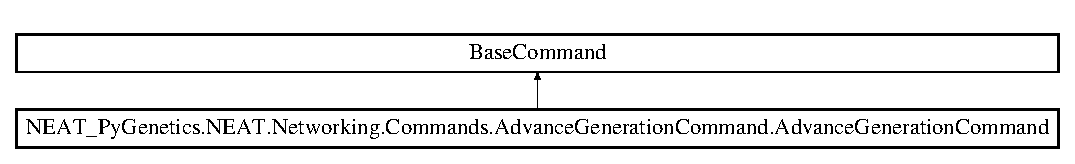
\includegraphics[height=1.758242cm]{class_n_e_a_t___py_genetics_1_1_n_e_a_t_1_1_networking_1_1_commands_1_1_advance_generation_comma5a5bfc6b55fe2df103ab75a9e3d9eebc}
\end{center}
\end{figure}
\subsection*{Public Member Functions}
\begin{DoxyCompactItemize}
\item 
def {\bfseries \+\_\+\+\_\+init\+\_\+\+\_\+} (self)\hypertarget{class_n_e_a_t___py_genetics_1_1_n_e_a_t_1_1_networking_1_1_commands_1_1_advance_generation_comma5a5bfc6b55fe2df103ab75a9e3d9eebc_aa5c2d4cae5b431359a0563a53f2e8020}{}\label{class_n_e_a_t___py_genetics_1_1_n_e_a_t_1_1_networking_1_1_commands_1_1_advance_generation_comma5a5bfc6b55fe2df103ab75a9e3d9eebc_aa5c2d4cae5b431359a0563a53f2e8020}

\item 
def {\bfseries set\+\_\+advance\+\_\+generation}\hypertarget{class_n_e_a_t___py_genetics_1_1_n_e_a_t_1_1_networking_1_1_commands_1_1_advance_generation_comma5a5bfc6b55fe2df103ab75a9e3d9eebc_a2d1945cf45fc83a8fc73aa690829969d}{}\label{class_n_e_a_t___py_genetics_1_1_n_e_a_t_1_1_networking_1_1_commands_1_1_advance_generation_comma5a5bfc6b55fe2df103ab75a9e3d9eebc_a2d1945cf45fc83a8fc73aa690829969d}

\end{DoxyCompactItemize}


\subsection{Detailed Description}


Definition at line 3 of file Advance\+Generation\+Command.\+py.



The documentation for this class was generated from the following file\+:\begin{DoxyCompactItemize}
\item 
N\+E\+A\+T/\+Networking/\+Commands/Advance\+Generation\+Command.\+py\end{DoxyCompactItemize}

\hypertarget{class_n_e_a_t___py_genetics_1_1_n_e_a_t_1_1_genome_structures_1_1_analysis_structure_1_1_analysis_genome_1_1_analysis_genome}{}\section{N\+E\+A\+T\+\_\+\+Py\+Genetics.\+N\+E\+A\+T.\+Genome\+Structures.\+Analysis\+Structure.\+Analysis\+Genome.\+Analysis\+Genome Class Reference}
\label{class_n_e_a_t___py_genetics_1_1_n_e_a_t_1_1_genome_structures_1_1_analysis_structure_1_1_analysis_genome_1_1_analysis_genome}\index{N\+E\+A\+T\+\_\+\+Py\+Genetics.\+N\+E\+A\+T.\+Genome\+Structures.\+Analysis\+Structure.\+Analysis\+Genome.\+Analysis\+Genome@{N\+E\+A\+T\+\_\+\+Py\+Genetics.\+N\+E\+A\+T.\+Genome\+Structures.\+Analysis\+Structure.\+Analysis\+Genome.\+Analysis\+Genome}}
Inheritance diagram for N\+E\+A\+T\+\_\+\+Py\+Genetics.\+N\+E\+A\+T.\+Genome\+Structures.\+Analysis\+Structure.\+Analysis\+Genome.\+Analysis\+Genome\+:\begin{figure}[H]
\begin{center}
\leavevmode
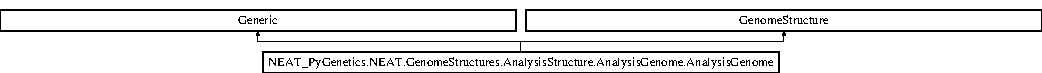
\includegraphics[height=0.984183cm]{class_n_e_a_t___py_genetics_1_1_n_e_a_t_1_1_genome_structures_1_1_analysis_structure_1_1_analysis_genome_1_1_analysis_genome}
\end{center}
\end{figure}
\subsection*{Public Member Functions}
\begin{DoxyCompactItemize}
\item 
def {\bfseries \+\_\+\+\_\+init\+\_\+\+\_\+}\hypertarget{class_n_e_a_t___py_genetics_1_1_n_e_a_t_1_1_genome_structures_1_1_analysis_structure_1_1_analysis_genome_1_1_analysis_genome_ade327b90f0ad5077a0864d5a7dfe705e}{}\label{class_n_e_a_t___py_genetics_1_1_n_e_a_t_1_1_genome_structures_1_1_analysis_structure_1_1_analysis_genome_1_1_analysis_genome_ade327b90f0ad5077a0864d5a7dfe705e}

\item 
def {\bfseries input\+\_\+nodes} (self)\hypertarget{class_n_e_a_t___py_genetics_1_1_n_e_a_t_1_1_genome_structures_1_1_analysis_structure_1_1_analysis_genome_1_1_analysis_genome_afde7a1abfb35596b72a79b5a1119acfd}{}\label{class_n_e_a_t___py_genetics_1_1_n_e_a_t_1_1_genome_structures_1_1_analysis_structure_1_1_analysis_genome_1_1_analysis_genome_afde7a1abfb35596b72a79b5a1119acfd}

\item 
def {\bfseries output\+\_\+nodes} (self)\hypertarget{class_n_e_a_t___py_genetics_1_1_n_e_a_t_1_1_genome_structures_1_1_analysis_structure_1_1_analysis_genome_1_1_analysis_genome_afd38f7e3e579713434e6f7ad977ace57}{}\label{class_n_e_a_t___py_genetics_1_1_n_e_a_t_1_1_genome_structures_1_1_analysis_structure_1_1_analysis_genome_1_1_analysis_genome_afd38f7e3e579713434e6f7ad977ace57}

\item 
def {\bfseries nodes} (self)\hypertarget{class_n_e_a_t___py_genetics_1_1_n_e_a_t_1_1_genome_structures_1_1_analysis_structure_1_1_analysis_genome_1_1_analysis_genome_a249bc4c5e9cbf9f5f4e9c7c4d6dcfc4b}{}\label{class_n_e_a_t___py_genetics_1_1_n_e_a_t_1_1_genome_structures_1_1_analysis_structure_1_1_analysis_genome_1_1_analysis_genome_a249bc4c5e9cbf9f5f4e9c7c4d6dcfc4b}

\item 
def {\bfseries edges} (self)\hypertarget{class_n_e_a_t___py_genetics_1_1_n_e_a_t_1_1_genome_structures_1_1_analysis_structure_1_1_analysis_genome_1_1_analysis_genome_a4435fda98d49756abec987840f902abb}{}\label{class_n_e_a_t___py_genetics_1_1_n_e_a_t_1_1_genome_structures_1_1_analysis_structure_1_1_analysis_genome_1_1_analysis_genome_a4435fda98d49756abec987840f902abb}

\item 
def {\bfseries initialised} (self)\hypertarget{class_n_e_a_t___py_genetics_1_1_n_e_a_t_1_1_genome_structures_1_1_analysis_structure_1_1_analysis_genome_1_1_analysis_genome_a0fead92350d58b2f5f078e7fa54e19e0}{}\label{class_n_e_a_t___py_genetics_1_1_n_e_a_t_1_1_genome_structures_1_1_analysis_structure_1_1_analysis_genome_1_1_analysis_genome_a0fead92350d58b2f5f078e7fa54e19e0}

\end{DoxyCompactItemize}
\subsection*{Static Public Attributes}
\begin{DoxyCompactItemize}
\item 
{\bfseries head}\hypertarget{class_n_e_a_t___py_genetics_1_1_n_e_a_t_1_1_genome_structures_1_1_analysis_structure_1_1_analysis_genome_1_1_analysis_genome_a0738164ade43882c355f33037d133280}{}\label{class_n_e_a_t___py_genetics_1_1_n_e_a_t_1_1_genome_structures_1_1_analysis_structure_1_1_analysis_genome_1_1_analysis_genome_a0738164ade43882c355f33037d133280}

\item 
{\bfseries tail}\hypertarget{class_n_e_a_t___py_genetics_1_1_n_e_a_t_1_1_genome_structures_1_1_analysis_structure_1_1_analysis_genome_1_1_analysis_genome_a41704621b0d39e8476b95141dd1cf18d}{}\label{class_n_e_a_t___py_genetics_1_1_n_e_a_t_1_1_genome_structures_1_1_analysis_structure_1_1_analysis_genome_1_1_analysis_genome_a41704621b0d39e8476b95141dd1cf18d}

\end{DoxyCompactItemize}


\subsection{Detailed Description}
\begin{DoxyVerb}Data structure used for analysing genome graphs.
It uses an adjacency list representation of the genome graph
which is compatible with well known graph algorithms.
\end{DoxyVerb}
 

Definition at line 15 of file Analysis\+Genome.\+py.



The documentation for this class was generated from the following file\+:\begin{DoxyCompactItemize}
\item 
N\+E\+A\+T/\+Genome\+Structures/\+Analysis\+Structure/Analysis\+Genome.\+py\end{DoxyCompactItemize}

\hypertarget{class_n_e_a_t___py_genetics_1_1_n_e_a_t_1_1_analyst_1_1_analysis_result_1_1_analysis_result}{}\section{N\+E\+A\+T\+\_\+\+Py\+Genetics.\+N\+E\+A\+T.\+Analyst.\+Analysis\+Result.\+Analysis\+Result Class Reference}
\label{class_n_e_a_t___py_genetics_1_1_n_e_a_t_1_1_analyst_1_1_analysis_result_1_1_analysis_result}\index{N\+E\+A\+T\+\_\+\+Py\+Genetics.\+N\+E\+A\+T.\+Analyst.\+Analysis\+Result.\+Analysis\+Result@{N\+E\+A\+T\+\_\+\+Py\+Genetics.\+N\+E\+A\+T.\+Analyst.\+Analysis\+Result.\+Analysis\+Result}}
Inheritance diagram for N\+E\+A\+T\+\_\+\+Py\+Genetics.\+N\+E\+A\+T.\+Analyst.\+Analysis\+Result.\+Analysis\+Result\+:\begin{figure}[H]
\begin{center}
\leavevmode
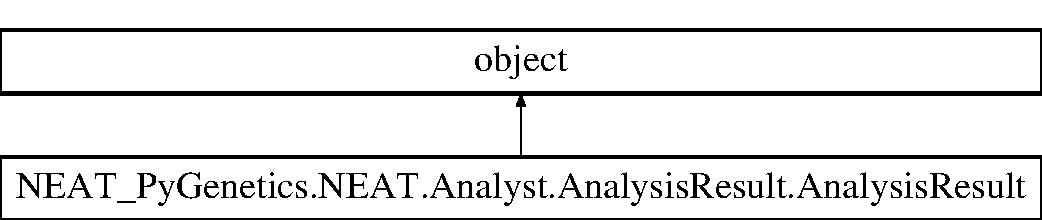
\includegraphics[height=2.000000cm]{class_n_e_a_t___py_genetics_1_1_n_e_a_t_1_1_analyst_1_1_analysis_result_1_1_analysis_result}
\end{center}
\end{figure}
\subsection*{Public Member Functions}
\begin{DoxyCompactItemize}
\item 
def {\bfseries \+\_\+\+\_\+init\+\_\+\+\_\+}\hypertarget{class_n_e_a_t___py_genetics_1_1_n_e_a_t_1_1_analyst_1_1_analysis_result_1_1_analysis_result_a76e2ba4c3bec7e93ab1c78e281a8504d}{}\label{class_n_e_a_t___py_genetics_1_1_n_e_a_t_1_1_analyst_1_1_analysis_result_1_1_analysis_result_a76e2ba4c3bec7e93ab1c78e281a8504d}

\item 
def {\bfseries \+\_\+\+\_\+eq\+\_\+\+\_\+}\hypertarget{class_n_e_a_t___py_genetics_1_1_n_e_a_t_1_1_analyst_1_1_analysis_result_1_1_analysis_result_a6145154aa0f23413e57312a78cc12f91}{}\label{class_n_e_a_t___py_genetics_1_1_n_e_a_t_1_1_analyst_1_1_analysis_result_1_1_analysis_result_a6145154aa0f23413e57312a78cc12f91}

\item 
def {\bfseries clear} (self)\hypertarget{class_n_e_a_t___py_genetics_1_1_n_e_a_t_1_1_analyst_1_1_analysis_result_1_1_analysis_result_abc4627be334a397f27b8173cb4a21796}{}\label{class_n_e_a_t___py_genetics_1_1_n_e_a_t_1_1_analyst_1_1_analysis_result_1_1_analysis_result_abc4627be334a397f27b8173cb4a21796}

\item 
def {\bfseries cycle\+\_\+nodes} (self)\hypertarget{class_n_e_a_t___py_genetics_1_1_n_e_a_t_1_1_analyst_1_1_analysis_result_1_1_analysis_result_ad3a9bbe518536d18882346d8ee9dd28e}{}\label{class_n_e_a_t___py_genetics_1_1_n_e_a_t_1_1_analyst_1_1_analysis_result_1_1_analysis_result_ad3a9bbe518536d18882346d8ee9dd28e}

\end{DoxyCompactItemize}
\subsection*{Public Attributes}
\begin{DoxyCompactItemize}
\item 
{\bfseries gene\+\_\+closes\+\_\+cycle\+\_\+map}\hypertarget{class_n_e_a_t___py_genetics_1_1_n_e_a_t_1_1_analyst_1_1_analysis_result_1_1_analysis_result_a8ad8be788715b6298240055bbd835d5e}{}\label{class_n_e_a_t___py_genetics_1_1_n_e_a_t_1_1_analyst_1_1_analysis_result_1_1_analysis_result_a8ad8be788715b6298240055bbd835d5e}

\item 
{\bfseries topologically\+\_\+sorted\+\_\+nodes}\hypertarget{class_n_e_a_t___py_genetics_1_1_n_e_a_t_1_1_analyst_1_1_analysis_result_1_1_analysis_result_a5dec17c624dfc418d21b543b366413e2}{}\label{class_n_e_a_t___py_genetics_1_1_n_e_a_t_1_1_analyst_1_1_analysis_result_1_1_analysis_result_a5dec17c624dfc418d21b543b366413e2}

\item 
{\bfseries topologically\+\_\+sorted\+\_\+cycle\+\_\+nodes}\hypertarget{class_n_e_a_t___py_genetics_1_1_n_e_a_t_1_1_analyst_1_1_analysis_result_1_1_analysis_result_acca98f28e97dddad4c4ee0c86d499e58}{}\label{class_n_e_a_t___py_genetics_1_1_n_e_a_t_1_1_analyst_1_1_analysis_result_1_1_analysis_result_acca98f28e97dddad4c4ee0c86d499e58}

\end{DoxyCompactItemize}


\subsection{Detailed Description}
\begin{DoxyVerb}Object used to store results of graph analysis.

Attributes:
    gene_closes_cycle_map: a dict that consists of gene id's (ints) as keys
        a boolean value that is true, if the gene closes a circle in the a-
        nalyzed graph.
    topologically_sorted_nodes: a list of all nodes in the analyzed graph in
        topological order.
    topologically_sorted_cycle_nodes: a list of all cycle closing nodes (at
        the source of the closing edge) in topological order. This is a sub-
        set of topologically_sorted_nodes.
\end{DoxyVerb}
 

Definition at line 6 of file Analysis\+Result.\+py.



The documentation for this class was generated from the following file\+:\begin{DoxyCompactItemize}
\item 
N\+E\+A\+T/\+Analyst/Analysis\+Result.\+py\end{DoxyCompactItemize}

\hypertarget{class_n_e_a_t___py_genetics_1_1_n_e_a_t_1_1_networking_1_1_commands_1_1_announce_session_command_1_1_announce_session_command}{}\section{N\+E\+A\+T\+\_\+\+Py\+Genetics.\+N\+E\+A\+T.\+Networking.\+Commands.\+Announce\+Session\+Command.\+Announce\+Session\+Command Class Reference}
\label{class_n_e_a_t___py_genetics_1_1_n_e_a_t_1_1_networking_1_1_commands_1_1_announce_session_command_1_1_announce_session_command}\index{N\+E\+A\+T\+\_\+\+Py\+Genetics.\+N\+E\+A\+T.\+Networking.\+Commands.\+Announce\+Session\+Command.\+Announce\+Session\+Command@{N\+E\+A\+T\+\_\+\+Py\+Genetics.\+N\+E\+A\+T.\+Networking.\+Commands.\+Announce\+Session\+Command.\+Announce\+Session\+Command}}
Inheritance diagram for N\+E\+A\+T\+\_\+\+Py\+Genetics.\+N\+E\+A\+T.\+Networking.\+Commands.\+Announce\+Session\+Command.\+Announce\+Session\+Command\+:\begin{figure}[H]
\begin{center}
\leavevmode
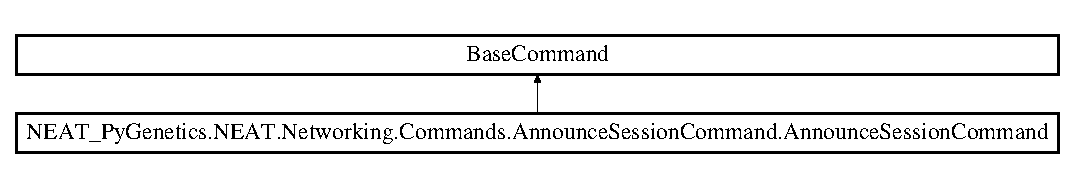
\includegraphics[height=1.821138cm]{class_n_e_a_t___py_genetics_1_1_n_e_a_t_1_1_networking_1_1_commands_1_1_announce_session_command_1_1_announce_session_command}
\end{center}
\end{figure}
\subsection*{Public Member Functions}
\begin{DoxyCompactItemize}
\item 
def {\bfseries \+\_\+\+\_\+init\+\_\+\+\_\+} (self)\hypertarget{class_n_e_a_t___py_genetics_1_1_n_e_a_t_1_1_networking_1_1_commands_1_1_announce_session_command_1_1_announce_session_command_a9ac1c2d236b717bc4b7ec521a7f3daa5}{}\label{class_n_e_a_t___py_genetics_1_1_n_e_a_t_1_1_networking_1_1_commands_1_1_announce_session_command_1_1_announce_session_command_a9ac1c2d236b717bc4b7ec521a7f3daa5}

\item 
def {\bfseries set\+\_\+config\+\_\+path} (self, config\+\_\+path)\hypertarget{class_n_e_a_t___py_genetics_1_1_n_e_a_t_1_1_networking_1_1_commands_1_1_announce_session_command_1_1_announce_session_command_ace39d5d011d61bb501f16f78ae1b4997}{}\label{class_n_e_a_t___py_genetics_1_1_n_e_a_t_1_1_networking_1_1_commands_1_1_announce_session_command_1_1_announce_session_command_ace39d5d011d61bb501f16f78ae1b4997}

\item 
def {\bfseries get\+\_\+config\+\_\+path} (self)\hypertarget{class_n_e_a_t___py_genetics_1_1_n_e_a_t_1_1_networking_1_1_commands_1_1_announce_session_command_1_1_announce_session_command_ade8f205209da28a137c8d361a4830c0b}{}\label{class_n_e_a_t___py_genetics_1_1_n_e_a_t_1_1_networking_1_1_commands_1_1_announce_session_command_1_1_announce_session_command_ade8f205209da28a137c8d361a4830c0b}

\item 
def {\bfseries set\+\_\+session\+\_\+id} (self, session\+\_\+id)\hypertarget{class_n_e_a_t___py_genetics_1_1_n_e_a_t_1_1_networking_1_1_commands_1_1_announce_session_command_1_1_announce_session_command_a7c9eae1dc5ba08c0b44182a6db99fd27}{}\label{class_n_e_a_t___py_genetics_1_1_n_e_a_t_1_1_networking_1_1_commands_1_1_announce_session_command_1_1_announce_session_command_a7c9eae1dc5ba08c0b44182a6db99fd27}

\item 
def {\bfseries get\+\_\+session\+\_\+id} (self)\hypertarget{class_n_e_a_t___py_genetics_1_1_n_e_a_t_1_1_networking_1_1_commands_1_1_announce_session_command_1_1_announce_session_command_a3e3a2c23ea1b303a4892f77895dd9350}{}\label{class_n_e_a_t___py_genetics_1_1_n_e_a_t_1_1_networking_1_1_commands_1_1_announce_session_command_1_1_announce_session_command_a3e3a2c23ea1b303a4892f77895dd9350}

\item 
def {\bfseries set\+\_\+block\+\_\+size}\hypertarget{class_n_e_a_t___py_genetics_1_1_n_e_a_t_1_1_networking_1_1_commands_1_1_announce_session_command_1_1_announce_session_command_a4b4d1a2f45cbe7e4be0658a3751e9dc3}{}\label{class_n_e_a_t___py_genetics_1_1_n_e_a_t_1_1_networking_1_1_commands_1_1_announce_session_command_1_1_announce_session_command_a4b4d1a2f45cbe7e4be0658a3751e9dc3}

\item 
def {\bfseries get\+\_\+block\+\_\+size} (self)\hypertarget{class_n_e_a_t___py_genetics_1_1_n_e_a_t_1_1_networking_1_1_commands_1_1_announce_session_command_1_1_announce_session_command_af6a3e5c83d5d990c909ef038272d797e}{}\label{class_n_e_a_t___py_genetics_1_1_n_e_a_t_1_1_networking_1_1_commands_1_1_announce_session_command_1_1_announce_session_command_af6a3e5c83d5d990c909ef038272d797e}

\end{DoxyCompactItemize}


\subsection{Detailed Description}


Definition at line 3 of file Announce\+Session\+Command.\+py.



The documentation for this class was generated from the following file\+:\begin{DoxyCompactItemize}
\item 
N\+E\+A\+T/\+Networking/\+Commands/Announce\+Session\+Command.\+py\end{DoxyCompactItemize}

\hypertarget{class_n_e_a_t___py_genetics_1_1_n_e_a_t_1_1_networking_1_1_commands_1_1_base_command_1_1_base_command}{}\section{N\+E\+A\+T\+\_\+\+Py\+Genetics.\+N\+E\+A\+T.\+Networking.\+Commands.\+Base\+Command.\+Base\+Command Class Reference}
\label{class_n_e_a_t___py_genetics_1_1_n_e_a_t_1_1_networking_1_1_commands_1_1_base_command_1_1_base_command}\index{N\+E\+A\+T\+\_\+\+Py\+Genetics.\+N\+E\+A\+T.\+Networking.\+Commands.\+Base\+Command.\+Base\+Command@{N\+E\+A\+T\+\_\+\+Py\+Genetics.\+N\+E\+A\+T.\+Networking.\+Commands.\+Base\+Command.\+Base\+Command}}
Inheritance diagram for N\+E\+A\+T\+\_\+\+Py\+Genetics.\+N\+E\+A\+T.\+Networking.\+Commands.\+Base\+Command.\+Base\+Command\+:\begin{figure}[H]
\begin{center}
\leavevmode
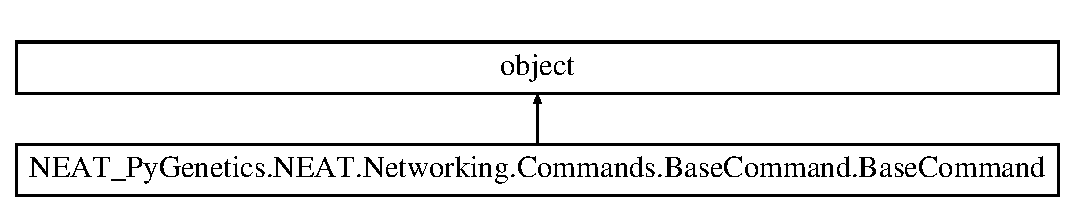
\includegraphics[height=2.000000cm]{class_n_e_a_t___py_genetics_1_1_n_e_a_t_1_1_networking_1_1_commands_1_1_base_command_1_1_base_command}
\end{center}
\end{figure}
\subsection*{Public Member Functions}
\begin{DoxyCompactItemize}
\item 
def {\bfseries \+\_\+\+\_\+init\+\_\+\+\_\+} (self)\hypertarget{class_n_e_a_t___py_genetics_1_1_n_e_a_t_1_1_networking_1_1_commands_1_1_base_command_1_1_base_command_a7f060792cc1f8ea526bc47c592eae10e}{}\label{class_n_e_a_t___py_genetics_1_1_n_e_a_t_1_1_networking_1_1_commands_1_1_base_command_1_1_base_command_a7f060792cc1f8ea526bc47c592eae10e}

\item 
def {\bfseries from\+\_\+dict} (self, dictionary)\hypertarget{class_n_e_a_t___py_genetics_1_1_n_e_a_t_1_1_networking_1_1_commands_1_1_base_command_1_1_base_command_a7466f3e151d869df0c0680aeaabd5497}{}\label{class_n_e_a_t___py_genetics_1_1_n_e_a_t_1_1_networking_1_1_commands_1_1_base_command_1_1_base_command_a7466f3e151d869df0c0680aeaabd5497}

\item 
def {\bfseries as\+\_\+dict} (self)\hypertarget{class_n_e_a_t___py_genetics_1_1_n_e_a_t_1_1_networking_1_1_commands_1_1_base_command_1_1_base_command_af8833907610ee782bbf991be49efe73f}{}\label{class_n_e_a_t___py_genetics_1_1_n_e_a_t_1_1_networking_1_1_commands_1_1_base_command_1_1_base_command_af8833907610ee782bbf991be49efe73f}

\item 
def {\bfseries acknowledged} (self)\hypertarget{class_n_e_a_t___py_genetics_1_1_n_e_a_t_1_1_networking_1_1_commands_1_1_base_command_1_1_base_command_a255f188c1306814a7840d33dfcf7650c}{}\label{class_n_e_a_t___py_genetics_1_1_n_e_a_t_1_1_networking_1_1_commands_1_1_base_command_1_1_base_command_a255f188c1306814a7840d33dfcf7650c}

\item 
def {\bfseries type} (self)\hypertarget{class_n_e_a_t___py_genetics_1_1_n_e_a_t_1_1_networking_1_1_commands_1_1_base_command_1_1_base_command_a631800c4e60223cee2fed6930a7b47df}{}\label{class_n_e_a_t___py_genetics_1_1_n_e_a_t_1_1_networking_1_1_commands_1_1_base_command_1_1_base_command_a631800c4e60223cee2fed6930a7b47df}

\item 
def {\bfseries \+\_\+\+\_\+eq\+\_\+\+\_\+}\hypertarget{class_n_e_a_t___py_genetics_1_1_n_e_a_t_1_1_networking_1_1_commands_1_1_base_command_1_1_base_command_ae1b33bc9a9dad6bcb9f2d3bb28c7355f}{}\label{class_n_e_a_t___py_genetics_1_1_n_e_a_t_1_1_networking_1_1_commands_1_1_base_command_1_1_base_command_ae1b33bc9a9dad6bcb9f2d3bb28c7355f}

\end{DoxyCompactItemize}
\subsection*{Public Attributes}
\begin{DoxyCompactItemize}
\item 
{\bfseries parameters}\hypertarget{class_n_e_a_t___py_genetics_1_1_n_e_a_t_1_1_networking_1_1_commands_1_1_base_command_1_1_base_command_a50465fec7d23d12cfca6cd0d8b6b8a67}{}\label{class_n_e_a_t___py_genetics_1_1_n_e_a_t_1_1_networking_1_1_commands_1_1_base_command_1_1_base_command_a50465fec7d23d12cfca6cd0d8b6b8a67}

\item 
{\bfseries result}\hypertarget{class_n_e_a_t___py_genetics_1_1_n_e_a_t_1_1_networking_1_1_commands_1_1_base_command_1_1_base_command_aa3136732344967769c806b465e699858}{}\label{class_n_e_a_t___py_genetics_1_1_n_e_a_t_1_1_networking_1_1_commands_1_1_base_command_1_1_base_command_aa3136732344967769c806b465e699858}

\end{DoxyCompactItemize}


\subsection{Detailed Description}


Definition at line 1 of file Base\+Command.\+py.



The documentation for this class was generated from the following file\+:\begin{DoxyCompactItemize}
\item 
N\+E\+A\+T/\+Networking/\+Commands/Base\+Command.\+py\end{DoxyCompactItemize}

\hypertarget{class_n_e_a_t___py_genetics_1_1_n_e_a_t_1_1_generator_1_1_breeder_1_1_breeder}{}\section{N\+E\+A\+T\+\_\+\+Py\+Genetics.\+N\+E\+A\+T.\+Generator.\+Breeder.\+Breeder Class Reference}
\label{class_n_e_a_t___py_genetics_1_1_n_e_a_t_1_1_generator_1_1_breeder_1_1_breeder}\index{N\+E\+A\+T\+\_\+\+Py\+Genetics.\+N\+E\+A\+T.\+Generator.\+Breeder.\+Breeder@{N\+E\+A\+T\+\_\+\+Py\+Genetics.\+N\+E\+A\+T.\+Generator.\+Breeder.\+Breeder}}
Inheritance diagram for N\+E\+A\+T\+\_\+\+Py\+Genetics.\+N\+E\+A\+T.\+Generator.\+Breeder.\+Breeder\+:\begin{figure}[H]
\begin{center}
\leavevmode
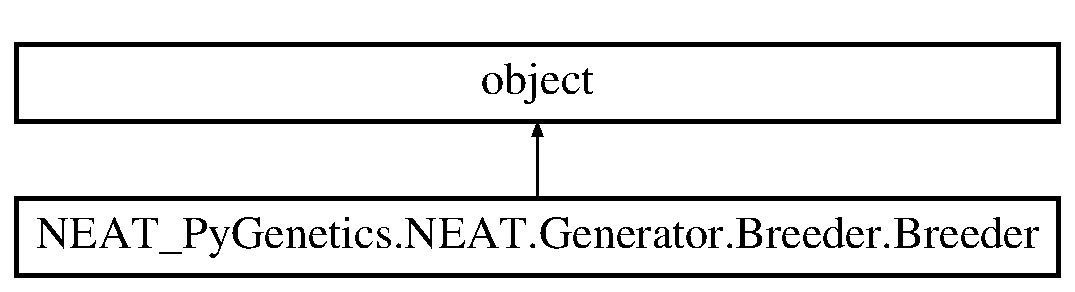
\includegraphics[height=2.000000cm]{class_n_e_a_t___py_genetics_1_1_n_e_a_t_1_1_generator_1_1_breeder_1_1_breeder}
\end{center}
\end{figure}
\subsection*{Public Member Functions}
\begin{DoxyCompactItemize}
\item 
def {\bfseries \+\_\+\+\_\+init\+\_\+\+\_\+}\hypertarget{class_n_e_a_t___py_genetics_1_1_n_e_a_t_1_1_generator_1_1_breeder_1_1_breeder_a99ffddd6afb3f995598605e165772515}{}\label{class_n_e_a_t___py_genetics_1_1_n_e_a_t_1_1_generator_1_1_breeder_1_1_breeder_a99ffddd6afb3f995598605e165772515}

\item 
def {\bfseries breed\+\_\+genomes}\hypertarget{class_n_e_a_t___py_genetics_1_1_n_e_a_t_1_1_generator_1_1_breeder_1_1_breeder_a6e78ccec465831c858910b1319e75076}{}\label{class_n_e_a_t___py_genetics_1_1_n_e_a_t_1_1_generator_1_1_breeder_1_1_breeder_a6e78ccec465831c858910b1319e75076}

\item 
def \hyperlink{class_n_e_a_t___py_genetics_1_1_n_e_a_t_1_1_generator_1_1_breeder_1_1_breeder_a761995541d6d9ff88e2ee112a57dff0f}{should\+\_\+gene\+\_\+be\+\_\+enabled} (self, instance\+\_\+one, instance\+\_\+two=None)
\end{DoxyCompactItemize}
\subsection*{Static Public Attributes}
\begin{DoxyCompactItemize}
\item 
{\bfseries breeding\+\_\+parameters}\hypertarget{class_n_e_a_t___py_genetics_1_1_n_e_a_t_1_1_generator_1_1_breeder_1_1_breeder_a0e28efbae8c7fdce0a0c0f1b7c7abe02}{}\label{class_n_e_a_t___py_genetics_1_1_n_e_a_t_1_1_generator_1_1_breeder_1_1_breeder_a0e28efbae8c7fdce0a0c0f1b7c7abe02}

\item 
{\bfseries bigger\+\_\+genome}\hypertarget{class_n_e_a_t___py_genetics_1_1_n_e_a_t_1_1_generator_1_1_breeder_1_1_breeder_a4b2204333e2b891725b9d7eac0f9533b}{}\label{class_n_e_a_t___py_genetics_1_1_n_e_a_t_1_1_generator_1_1_breeder_1_1_breeder_a4b2204333e2b891725b9d7eac0f9533b}

\item 
{\bfseries smaller\+\_\+genome}\hypertarget{class_n_e_a_t___py_genetics_1_1_n_e_a_t_1_1_generator_1_1_breeder_1_1_breeder_aee42ab257302cbcf2e6619111289c489}{}\label{class_n_e_a_t___py_genetics_1_1_n_e_a_t_1_1_generator_1_1_breeder_1_1_breeder_aee42ab257302cbcf2e6619111289c489}

\item 
{\bfseries bigger\+\_\+genome\+\_\+gene\+\_\+ids}\hypertarget{class_n_e_a_t___py_genetics_1_1_n_e_a_t_1_1_generator_1_1_breeder_1_1_breeder_aae86e270174a1ddc14677a5bd267ceda}{}\label{class_n_e_a_t___py_genetics_1_1_n_e_a_t_1_1_generator_1_1_breeder_1_1_breeder_aae86e270174a1ddc14677a5bd267ceda}

\item 
{\bfseries smaller\+\_\+genome\+\_\+gene\+\_\+ids}\hypertarget{class_n_e_a_t___py_genetics_1_1_n_e_a_t_1_1_generator_1_1_breeder_1_1_breeder_a1b7a43f5e5d325a0581e90e5666cc424}{}\label{class_n_e_a_t___py_genetics_1_1_n_e_a_t_1_1_generator_1_1_breeder_1_1_breeder_a1b7a43f5e5d325a0581e90e5666cc424}

\item 
{\bfseries all\+\_\+gene\+\_\+ids}\hypertarget{class_n_e_a_t___py_genetics_1_1_n_e_a_t_1_1_generator_1_1_breeder_1_1_breeder_aafd044323f51754e3d3ed1c56398b88b}{}\label{class_n_e_a_t___py_genetics_1_1_n_e_a_t_1_1_generator_1_1_breeder_1_1_breeder_aafd044323f51754e3d3ed1c56398b88b}

\item 
{\bfseries matching\+\_\+gene\+\_\+ids}\hypertarget{class_n_e_a_t___py_genetics_1_1_n_e_a_t_1_1_generator_1_1_breeder_1_1_breeder_a017b63dcfc04f983f3097f52d1b2ba80}{}\label{class_n_e_a_t___py_genetics_1_1_n_e_a_t_1_1_generator_1_1_breeder_1_1_breeder_a017b63dcfc04f983f3097f52d1b2ba80}

\item 
{\bfseries differing\+\_\+gene\+\_\+ids}\hypertarget{class_n_e_a_t___py_genetics_1_1_n_e_a_t_1_1_generator_1_1_breeder_1_1_breeder_a3ef5f23263b2205639606d0c9756e79c}{}\label{class_n_e_a_t___py_genetics_1_1_n_e_a_t_1_1_generator_1_1_breeder_1_1_breeder_a3ef5f23263b2205639606d0c9756e79c}

\item 
{\bfseries fitter\+\_\+genome\+\_\+table}\hypertarget{class_n_e_a_t___py_genetics_1_1_n_e_a_t_1_1_generator_1_1_breeder_1_1_breeder_a6898cc6d6a36379227d5a00f9e627432}{}\label{class_n_e_a_t___py_genetics_1_1_n_e_a_t_1_1_generator_1_1_breeder_1_1_breeder_a6898cc6d6a36379227d5a00f9e627432}

\item 
{\bfseries new\+\_\+genome}\hypertarget{class_n_e_a_t___py_genetics_1_1_n_e_a_t_1_1_generator_1_1_breeder_1_1_breeder_a8ecfda7d3fcfc166577e07cc977fa9cb}{}\label{class_n_e_a_t___py_genetics_1_1_n_e_a_t_1_1_generator_1_1_breeder_1_1_breeder_a8ecfda7d3fcfc166577e07cc977fa9cb}

\item 
{\bfseries parent\+\_\+genome\+\_\+table}\hypertarget{class_n_e_a_t___py_genetics_1_1_n_e_a_t_1_1_generator_1_1_breeder_1_1_breeder_a57dfe8e0f1eff1f6ef84492bc845dd40}{}\label{class_n_e_a_t___py_genetics_1_1_n_e_a_t_1_1_generator_1_1_breeder_1_1_breeder_a57dfe8e0f1eff1f6ef84492bc845dd40}

\item 
{\bfseries gene\+\_\+enabled}\hypertarget{class_n_e_a_t___py_genetics_1_1_n_e_a_t_1_1_generator_1_1_breeder_1_1_breeder_a11f9b1f5d4b9804dd8b54db956734938}{}\label{class_n_e_a_t___py_genetics_1_1_n_e_a_t_1_1_generator_1_1_breeder_1_1_breeder_a11f9b1f5d4b9804dd8b54db956734938}

\item 
{\bfseries gene\+\_\+weight}\hypertarget{class_n_e_a_t___py_genetics_1_1_n_e_a_t_1_1_generator_1_1_breeder_1_1_breeder_a1e14b916370fa769ae820893190a1f28}{}\label{class_n_e_a_t___py_genetics_1_1_n_e_a_t_1_1_generator_1_1_breeder_1_1_breeder_a1e14b916370fa769ae820893190a1f28}

\item 
{\bfseries inherit\+\_\+gene}\hypertarget{class_n_e_a_t___py_genetics_1_1_n_e_a_t_1_1_generator_1_1_breeder_1_1_breeder_a82bb0cf6761460a4478abd22fc41e256}{}\label{class_n_e_a_t___py_genetics_1_1_n_e_a_t_1_1_generator_1_1_breeder_1_1_breeder_a82bb0cf6761460a4478abd22fc41e256}

\end{DoxyCompactItemize}


\subsection{Detailed Description}


Definition at line 7 of file Breeder.\+py.



\subsection{Member Function Documentation}
\index{N\+E\+A\+T\+\_\+\+Py\+Genetics\+::\+N\+E\+A\+T\+::\+Generator\+::\+Breeder\+::\+Breeder@{N\+E\+A\+T\+\_\+\+Py\+Genetics\+::\+N\+E\+A\+T\+::\+Generator\+::\+Breeder\+::\+Breeder}!should\+\_\+gene\+\_\+be\+\_\+enabled@{should\+\_\+gene\+\_\+be\+\_\+enabled}}
\index{should\+\_\+gene\+\_\+be\+\_\+enabled@{should\+\_\+gene\+\_\+be\+\_\+enabled}!N\+E\+A\+T\+\_\+\+Py\+Genetics\+::\+N\+E\+A\+T\+::\+Generator\+::\+Breeder\+::\+Breeder@{N\+E\+A\+T\+\_\+\+Py\+Genetics\+::\+N\+E\+A\+T\+::\+Generator\+::\+Breeder\+::\+Breeder}}
\subsubsection[{\texorpdfstring{should\+\_\+gene\+\_\+be\+\_\+enabled(self, instance\+\_\+one, instance\+\_\+two=\+None)}{should_gene_be_enabled(self, instance_one, instance_two=None)}}]{\setlength{\rightskip}{0pt plus 5cm}def N\+E\+A\+T\+\_\+\+Py\+Genetics.\+N\+E\+A\+T.\+Generator.\+Breeder.\+Breeder.\+should\+\_\+gene\+\_\+be\+\_\+enabled (
\begin{DoxyParamCaption}
\item[{}]{self, }
\item[{}]{instance\+\_\+one, }
\item[{}]{instance\+\_\+two = {\ttfamily None}}
\end{DoxyParamCaption}
)}\hypertarget{class_n_e_a_t___py_genetics_1_1_n_e_a_t_1_1_generator_1_1_breeder_1_1_breeder_a761995541d6d9ff88e2ee112a57dff0f}{}\label{class_n_e_a_t___py_genetics_1_1_n_e_a_t_1_1_generator_1_1_breeder_1_1_breeder_a761995541d6d9ff88e2ee112a57dff0f}
\begin{DoxyVerb}Decides whether the inherited variant of a gene should be
enabled in the offspring genome based on both parents' instances
of the gene.
:param instance_one: The first gene instance
:param instance_two:  The second gene instance
:return: Whether the inherited gene should be enabled
\end{DoxyVerb}
 

Definition at line 112 of file Breeder.\+py.



The documentation for this class was generated from the following file\+:\begin{DoxyCompactItemize}
\item 
N\+E\+A\+T/\+Generator/Breeder.\+py\end{DoxyCompactItemize}

\hypertarget{class_n_e_a_t___py_genetics_1_1_n_e_a_t_1_1_analyst_1_1_cluster_1_1_cluster}{}\section{N\+E\+A\+T\+\_\+\+Py\+Genetics.\+N\+E\+A\+T.\+Analyst.\+Cluster.\+Cluster Class Reference}
\label{class_n_e_a_t___py_genetics_1_1_n_e_a_t_1_1_analyst_1_1_cluster_1_1_cluster}\index{N\+E\+A\+T\+\_\+\+Py\+Genetics.\+N\+E\+A\+T.\+Analyst.\+Cluster.\+Cluster@{N\+E\+A\+T\+\_\+\+Py\+Genetics.\+N\+E\+A\+T.\+Analyst.\+Cluster.\+Cluster}}
Inheritance diagram for N\+E\+A\+T\+\_\+\+Py\+Genetics.\+N\+E\+A\+T.\+Analyst.\+Cluster.\+Cluster\+:\begin{figure}[H]
\begin{center}
\leavevmode
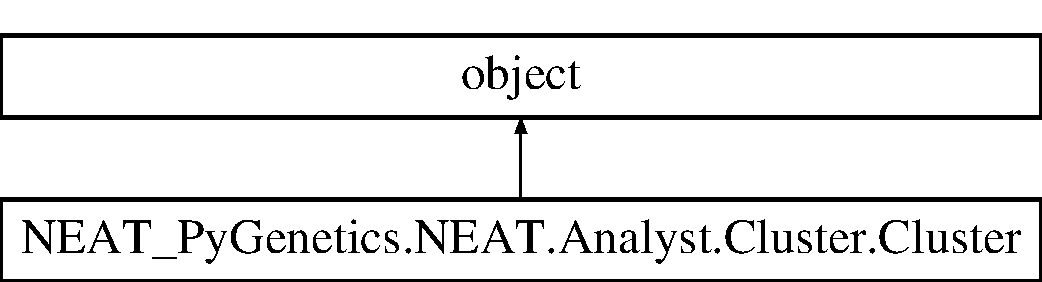
\includegraphics[height=2.000000cm]{class_n_e_a_t___py_genetics_1_1_n_e_a_t_1_1_analyst_1_1_cluster_1_1_cluster}
\end{center}
\end{figure}
\subsection*{Public Member Functions}
\begin{DoxyCompactItemize}
\item 
def {\bfseries \+\_\+\+\_\+init\+\_\+\+\_\+} (self)\hypertarget{class_n_e_a_t___py_genetics_1_1_n_e_a_t_1_1_analyst_1_1_cluster_1_1_cluster_a12ebc01de1535941e1af477dddaedbe9}{}\label{class_n_e_a_t___py_genetics_1_1_n_e_a_t_1_1_analyst_1_1_cluster_1_1_cluster_a12ebc01de1535941e1af477dddaedbe9}

\item 
def {\bfseries \+\_\+\+\_\+eq\+\_\+\+\_\+}\hypertarget{class_n_e_a_t___py_genetics_1_1_n_e_a_t_1_1_analyst_1_1_cluster_1_1_cluster_a85d2dfa24ff6846be17920a77987ece5}{}\label{class_n_e_a_t___py_genetics_1_1_n_e_a_t_1_1_analyst_1_1_cluster_1_1_cluster_a85d2dfa24ff6846be17920a77987ece5}

\item 
def {\bfseries cluster\+\_\+id} (self)\hypertarget{class_n_e_a_t___py_genetics_1_1_n_e_a_t_1_1_analyst_1_1_cluster_1_1_cluster_a691632bc1747f486a4f1c8fe3ee02265}{}\label{class_n_e_a_t___py_genetics_1_1_n_e_a_t_1_1_analyst_1_1_cluster_1_1_cluster_a691632bc1747f486a4f1c8fe3ee02265}

\end{DoxyCompactItemize}
\subsection*{Public Attributes}
\begin{DoxyCompactItemize}
\item 
{\bfseries representative}\hypertarget{class_n_e_a_t___py_genetics_1_1_n_e_a_t_1_1_analyst_1_1_cluster_1_1_cluster_a6d98b217b836b08679f9b20f9459f2ba}{}\label{class_n_e_a_t___py_genetics_1_1_n_e_a_t_1_1_analyst_1_1_cluster_1_1_cluster_a6d98b217b836b08679f9b20f9459f2ba}

\item 
{\bfseries fitness}\hypertarget{class_n_e_a_t___py_genetics_1_1_n_e_a_t_1_1_analyst_1_1_cluster_1_1_cluster_a1c956f56f9f8e92391eb6c8912d8cd8a}{}\label{class_n_e_a_t___py_genetics_1_1_n_e_a_t_1_1_analyst_1_1_cluster_1_1_cluster_a1c956f56f9f8e92391eb6c8912d8cd8a}

\item 
{\bfseries offspring}\hypertarget{class_n_e_a_t___py_genetics_1_1_n_e_a_t_1_1_analyst_1_1_cluster_1_1_cluster_a29316a5b5546bea6c97896e814ce084e}{}\label{class_n_e_a_t___py_genetics_1_1_n_e_a_t_1_1_analyst_1_1_cluster_1_1_cluster_a29316a5b5546bea6c97896e814ce084e}

\item 
{\bfseries alive}\hypertarget{class_n_e_a_t___py_genetics_1_1_n_e_a_t_1_1_analyst_1_1_cluster_1_1_cluster_a9d814ccf011d42ab14bdade4be3e1fdb}{}\label{class_n_e_a_t___py_genetics_1_1_n_e_a_t_1_1_analyst_1_1_cluster_1_1_cluster_a9d814ccf011d42ab14bdade4be3e1fdb}

\end{DoxyCompactItemize}


\subsection{Detailed Description}
\begin{DoxyVerb}Object used to represent a single cluster as stored
in the database.

Attributes:
    cluster_id (_id):
        The Cluster's ID, unique
    representative:
        The ID of the representative StorageGenome.
        All genomes in the cluster are topologically similar
        to it's representative genome.
    fitness:
        The cluster's fitness value.
        This is calculated from the fitness values of the
        contained genomes by a shared fitness approach.
    offspring:
        The amount of offspring that will be generated based
        on genomes from this clusters during the next generation.
    alive:
        Whether the cluster is alive, i.e. if there are any
        genomes in the current population which belong to this
        cluster.
\end{DoxyVerb}
 

Definition at line 4 of file Cluster.\+py.



The documentation for this class was generated from the following file\+:\begin{DoxyCompactItemize}
\item 
N\+E\+A\+T/\+Analyst/Cluster.\+py\end{DoxyCompactItemize}

\hypertarget{class_n_e_a_t___py_genetics_1_1_n_e_a_t_1_1_repository_1_1_cluster_repository_1_1_cluster_repository}{}\section{N\+E\+A\+T\+\_\+\+Py\+Genetics.\+N\+E\+A\+T.\+Repository.\+Cluster\+Repository.\+Cluster\+Repository Class Reference}
\label{class_n_e_a_t___py_genetics_1_1_n_e_a_t_1_1_repository_1_1_cluster_repository_1_1_cluster_repository}\index{N\+E\+A\+T\+\_\+\+Py\+Genetics.\+N\+E\+A\+T.\+Repository.\+Cluster\+Repository.\+Cluster\+Repository@{N\+E\+A\+T\+\_\+\+Py\+Genetics.\+N\+E\+A\+T.\+Repository.\+Cluster\+Repository.\+Cluster\+Repository}}
Inheritance diagram for N\+E\+A\+T\+\_\+\+Py\+Genetics.\+N\+E\+A\+T.\+Repository.\+Cluster\+Repository.\+Cluster\+Repository\+:\begin{figure}[H]
\begin{center}
\leavevmode
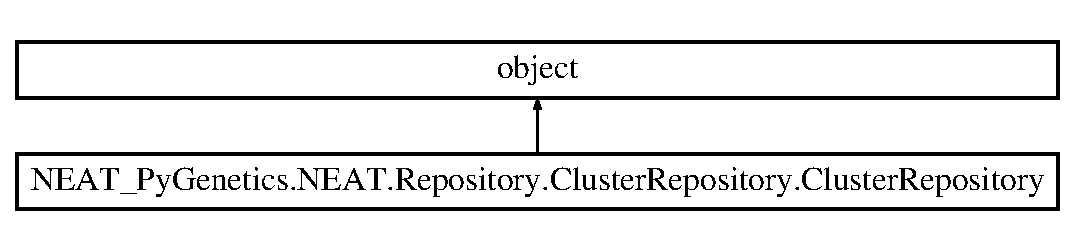
\includegraphics[height=2.000000cm]{class_n_e_a_t___py_genetics_1_1_n_e_a_t_1_1_repository_1_1_cluster_repository_1_1_cluster_repository}
\end{center}
\end{figure}
\subsection*{Public Member Functions}
\begin{DoxyCompactItemize}
\item 
def {\bfseries \+\_\+\+\_\+init\+\_\+\+\_\+}\hypertarget{class_n_e_a_t___py_genetics_1_1_n_e_a_t_1_1_repository_1_1_cluster_repository_1_1_cluster_repository_a49b3cd6db6131c52bba0de2481584f20}{}\label{class_n_e_a_t___py_genetics_1_1_n_e_a_t_1_1_repository_1_1_cluster_repository_1_1_cluster_repository_a49b3cd6db6131c52bba0de2481584f20}

\item 
def {\bfseries get\+\_\+current\+\_\+clusters} (self)\hypertarget{class_n_e_a_t___py_genetics_1_1_n_e_a_t_1_1_repository_1_1_cluster_repository_1_1_cluster_repository_a06b7a0bc3b6bf0ddc6eb9040dcecd74b}{}\label{class_n_e_a_t___py_genetics_1_1_n_e_a_t_1_1_repository_1_1_cluster_repository_1_1_cluster_repository_a06b7a0bc3b6bf0ddc6eb9040dcecd74b}

\item 
def {\bfseries add\+\_\+cluster\+\_\+with\+\_\+representative}\hypertarget{class_n_e_a_t___py_genetics_1_1_n_e_a_t_1_1_repository_1_1_cluster_repository_1_1_cluster_repository_adab9f634071749a11cfe0875075fb0a5}{}\label{class_n_e_a_t___py_genetics_1_1_n_e_a_t_1_1_repository_1_1_cluster_repository_1_1_cluster_repository_adab9f634071749a11cfe0875075fb0a5}

\item 
def {\bfseries archive\+\_\+cluster}\hypertarget{class_n_e_a_t___py_genetics_1_1_n_e_a_t_1_1_repository_1_1_cluster_repository_1_1_cluster_repository_a58649974b303a672e75c650e69d1cb21}{}\label{class_n_e_a_t___py_genetics_1_1_n_e_a_t_1_1_repository_1_1_cluster_repository_1_1_cluster_repository_a58649974b303a672e75c650e69d1cb21}

\item 
def {\bfseries get\+\_\+cluster\+\_\+by\+\_\+representative}\hypertarget{class_n_e_a_t___py_genetics_1_1_n_e_a_t_1_1_repository_1_1_cluster_repository_1_1_cluster_repository_af79b19639b87ae827067ddb4d23fe83d}{}\label{class_n_e_a_t___py_genetics_1_1_n_e_a_t_1_1_repository_1_1_cluster_repository_1_1_cluster_repository_af79b19639b87ae827067ddb4d23fe83d}

\item 
def {\bfseries get\+\_\+cluster\+\_\+count} (self)\hypertarget{class_n_e_a_t___py_genetics_1_1_n_e_a_t_1_1_repository_1_1_cluster_repository_1_1_cluster_repository_aba5e54a8cf88aece8ebb990b812a3ce2}{}\label{class_n_e_a_t___py_genetics_1_1_n_e_a_t_1_1_repository_1_1_cluster_repository_1_1_cluster_repository_aba5e54a8cf88aece8ebb990b812a3ce2}

\item 
def {\bfseries update\+\_\+offspring\+\_\+for\+\_\+cluster}\hypertarget{class_n_e_a_t___py_genetics_1_1_n_e_a_t_1_1_repository_1_1_cluster_repository_1_1_cluster_repository_a40254dd9f12511e8fa3e707b65938db4}{}\label{class_n_e_a_t___py_genetics_1_1_n_e_a_t_1_1_repository_1_1_cluster_repository_1_1_cluster_repository_a40254dd9f12511e8fa3e707b65938db4}

\item 
def {\bfseries update\+\_\+fitness\+\_\+for\+\_\+cluster}\hypertarget{class_n_e_a_t___py_genetics_1_1_n_e_a_t_1_1_repository_1_1_cluster_repository_1_1_cluster_repository_ac0949d637eb75abae63005db57f14700}{}\label{class_n_e_a_t___py_genetics_1_1_n_e_a_t_1_1_repository_1_1_cluster_repository_1_1_cluster_repository_ac0949d637eb75abae63005db57f14700}

\item 
def {\bfseries update\+\_\+max\+\_\+population\+\_\+for\+\_\+cluster}\hypertarget{class_n_e_a_t___py_genetics_1_1_n_e_a_t_1_1_repository_1_1_cluster_repository_1_1_cluster_repository_a69ed07f142ec57528a44026aba6bd1fe}{}\label{class_n_e_a_t___py_genetics_1_1_n_e_a_t_1_1_repository_1_1_cluster_repository_1_1_cluster_repository_a69ed07f142ec57528a44026aba6bd1fe}

\end{DoxyCompactItemize}
\subsection*{Static Public Attributes}
\begin{DoxyCompactItemize}
\item 
{\bfseries cluster}\hypertarget{class_n_e_a_t___py_genetics_1_1_n_e_a_t_1_1_repository_1_1_cluster_repository_1_1_cluster_repository_a1834515cd9dbbdf31e311ce6a2e8e78a}{}\label{class_n_e_a_t___py_genetics_1_1_n_e_a_t_1_1_repository_1_1_cluster_repository_1_1_cluster_repository_a1834515cd9dbbdf31e311ce6a2e8e78a}

\item 
{\bfseries representative}\hypertarget{class_n_e_a_t___py_genetics_1_1_n_e_a_t_1_1_repository_1_1_cluster_repository_1_1_cluster_repository_accef80a33d0dd0473ad8c9b3723ec0d9}{}\label{class_n_e_a_t___py_genetics_1_1_n_e_a_t_1_1_repository_1_1_cluster_repository_1_1_cluster_repository_accef80a33d0dd0473ad8c9b3723ec0d9}

\item 
{\bfseries offspring}\hypertarget{class_n_e_a_t___py_genetics_1_1_n_e_a_t_1_1_repository_1_1_cluster_repository_1_1_cluster_repository_a8d545f61188a41b15f2c7f3fb2fddcec}{}\label{class_n_e_a_t___py_genetics_1_1_n_e_a_t_1_1_repository_1_1_cluster_repository_1_1_cluster_repository_a8d545f61188a41b15f2c7f3fb2fddcec}

\end{DoxyCompactItemize}


\subsection{Detailed Description}


Definition at line 8 of file Cluster\+Repository.\+py.



The documentation for this class was generated from the following file\+:\begin{DoxyCompactItemize}
\item 
N\+E\+A\+T/\+Repository/Cluster\+Repository.\+py\end{DoxyCompactItemize}

\hypertarget{class_n_e_a_t___py_genetics_1_1_n_e_a_t_1_1_networking_1_1_commands_1_1_command_transcoder_1_1_command_transcoder}{}\section{N\+E\+A\+T\+\_\+\+Py\+Genetics.\+N\+E\+A\+T.\+Networking.\+Commands.\+Command\+Transcoder.\+Command\+Transcoder Class Reference}
\label{class_n_e_a_t___py_genetics_1_1_n_e_a_t_1_1_networking_1_1_commands_1_1_command_transcoder_1_1_command_transcoder}\index{N\+E\+A\+T\+\_\+\+Py\+Genetics.\+N\+E\+A\+T.\+Networking.\+Commands.\+Command\+Transcoder.\+Command\+Transcoder@{N\+E\+A\+T\+\_\+\+Py\+Genetics.\+N\+E\+A\+T.\+Networking.\+Commands.\+Command\+Transcoder.\+Command\+Transcoder}}
Inheritance diagram for N\+E\+A\+T\+\_\+\+Py\+Genetics.\+N\+E\+A\+T.\+Networking.\+Commands.\+Command\+Transcoder.\+Command\+Transcoder\+:\begin{figure}[H]
\begin{center}
\leavevmode
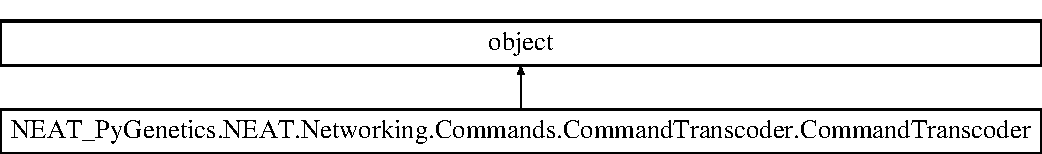
\includegraphics[height=2.000000cm]{class_n_e_a_t___py_genetics_1_1_n_e_a_t_1_1_networking_1_1_commands_1_1_command_transcoder_1_1_command_transcoder}
\end{center}
\end{figure}
\subsection*{Static Public Member Functions}
\begin{DoxyCompactItemize}
\item 
def {\bfseries encode\+\_\+command}\hypertarget{class_n_e_a_t___py_genetics_1_1_n_e_a_t_1_1_networking_1_1_commands_1_1_command_transcoder_1_1_command_transcoder_a173c5fa30eabf9dc236f761803dfd1df}{}\label{class_n_e_a_t___py_genetics_1_1_n_e_a_t_1_1_networking_1_1_commands_1_1_command_transcoder_1_1_command_transcoder_a173c5fa30eabf9dc236f761803dfd1df}

\item 
def {\bfseries decode\+\_\+command}\hypertarget{class_n_e_a_t___py_genetics_1_1_n_e_a_t_1_1_networking_1_1_commands_1_1_command_transcoder_1_1_command_transcoder_aebdcf1865dd3c040c341f00e88c8d387}{}\label{class_n_e_a_t___py_genetics_1_1_n_e_a_t_1_1_networking_1_1_commands_1_1_command_transcoder_1_1_command_transcoder_aebdcf1865dd3c040c341f00e88c8d387}

\end{DoxyCompactItemize}
\subsection*{Static Public Attributes}
\begin{DoxyCompactItemize}
\item 
{\bfseries type\+\_\+class\+\_\+map}\hypertarget{class_n_e_a_t___py_genetics_1_1_n_e_a_t_1_1_networking_1_1_commands_1_1_command_transcoder_1_1_command_transcoder_a161a64d3c2586008802d174ebc5b6e4b}{}\label{class_n_e_a_t___py_genetics_1_1_n_e_a_t_1_1_networking_1_1_commands_1_1_command_transcoder_1_1_command_transcoder_a161a64d3c2586008802d174ebc5b6e4b}

\end{DoxyCompactItemize}


\subsection{Detailed Description}


Definition at line 5 of file Command\+Transcoder.\+py.



The documentation for this class was generated from the following file\+:\begin{DoxyCompactItemize}
\item 
N\+E\+A\+T/\+Networking/\+Commands/Command\+Transcoder.\+py\end{DoxyCompactItemize}

\hypertarget{class_n_e_a_t___py_genetics_1_1_n_e_a_t_1_1_genome_structures_1_1_simulation_structure_1_1_simulation_nodes_1_1_cycle_node}{}\section{N\+E\+A\+T\+\_\+\+Py\+Genetics.\+N\+E\+A\+T.\+Genome\+Structures.\+Simulation\+Structure.\+Simulation\+Nodes.\+Cycle\+Node Class Reference}
\label{class_n_e_a_t___py_genetics_1_1_n_e_a_t_1_1_genome_structures_1_1_simulation_structure_1_1_simulation_nodes_1_1_cycle_node}\index{N\+E\+A\+T\+\_\+\+Py\+Genetics.\+N\+E\+A\+T.\+Genome\+Structures.\+Simulation\+Structure.\+Simulation\+Nodes.\+Cycle\+Node@{N\+E\+A\+T\+\_\+\+Py\+Genetics.\+N\+E\+A\+T.\+Genome\+Structures.\+Simulation\+Structure.\+Simulation\+Nodes.\+Cycle\+Node}}
Inheritance diagram for N\+E\+A\+T\+\_\+\+Py\+Genetics.\+N\+E\+A\+T.\+Genome\+Structures.\+Simulation\+Structure.\+Simulation\+Nodes.\+Cycle\+Node\+:\begin{figure}[H]
\begin{center}
\leavevmode
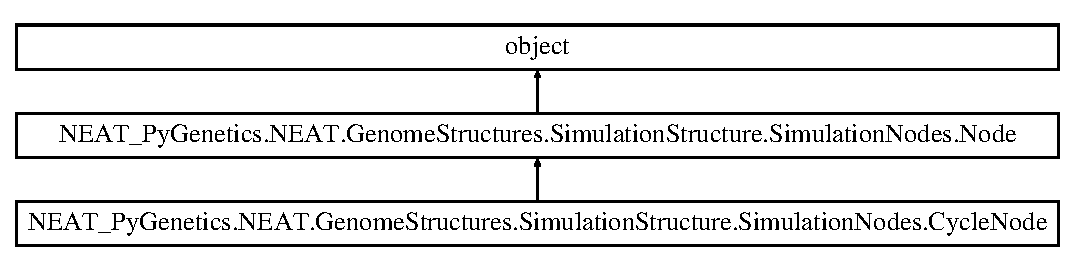
\includegraphics[height=3.000000cm]{class_n_e_a_t___py_genetics_1_1_n_e_a_t_1_1_genome_structures_1_1_simulation_structure_1_1_simulation_nodes_1_1_cycle_node}
\end{center}
\end{figure}
\subsection*{Public Member Functions}
\begin{DoxyCompactItemize}
\item 
def {\bfseries \+\_\+\+\_\+init\+\_\+\+\_\+}\hypertarget{class_n_e_a_t___py_genetics_1_1_n_e_a_t_1_1_genome_structures_1_1_simulation_structure_1_1_simulation_nodes_1_1_cycle_node_a7296250c1afe722523e7897b0ab2b4d4}{}\label{class_n_e_a_t___py_genetics_1_1_n_e_a_t_1_1_genome_structures_1_1_simulation_structure_1_1_simulation_nodes_1_1_cycle_node_a7296250c1afe722523e7897b0ab2b4d4}

\item 
def {\bfseries add\+\_\+cycle\+\_\+successor}\hypertarget{class_n_e_a_t___py_genetics_1_1_n_e_a_t_1_1_genome_structures_1_1_simulation_structure_1_1_simulation_nodes_1_1_cycle_node_acac910243feebfd38ee9bb9503a4db24}{}\label{class_n_e_a_t___py_genetics_1_1_n_e_a_t_1_1_genome_structures_1_1_simulation_structure_1_1_simulation_nodes_1_1_cycle_node_acac910243feebfd38ee9bb9503a4db24}

\item 
def {\bfseries add\+\_\+cycle\+\_\+successors}\hypertarget{class_n_e_a_t___py_genetics_1_1_n_e_a_t_1_1_genome_structures_1_1_simulation_structure_1_1_simulation_nodes_1_1_cycle_node_a842b0166427a3d54ba9dc87062d2cd57}{}\label{class_n_e_a_t___py_genetics_1_1_n_e_a_t_1_1_genome_structures_1_1_simulation_structure_1_1_simulation_nodes_1_1_cycle_node_a842b0166427a3d54ba9dc87062d2cd57}

\item 
def \hyperlink{class_n_e_a_t___py_genetics_1_1_n_e_a_t_1_1_genome_structures_1_1_simulation_structure_1_1_simulation_nodes_1_1_cycle_node_aded4c01be2b30e8fc2d0bd89bd4d9763}{fire\+\_\+cycles} (self)
\item 
def \hyperlink{class_n_e_a_t___py_genetics_1_1_n_e_a_t_1_1_genome_structures_1_1_simulation_structure_1_1_simulation_nodes_1_1_cycle_node_a55f0110c03f18c3b093f7cb06354e1e3}{preserve\+\_\+memory} (self)
\end{DoxyCompactItemize}
\subsection*{Static Public Attributes}
\begin{DoxyCompactItemize}
\item 
{\bfseries cycle\+\_\+successors}\hypertarget{class_n_e_a_t___py_genetics_1_1_n_e_a_t_1_1_genome_structures_1_1_simulation_structure_1_1_simulation_nodes_1_1_cycle_node_a1af1cde360e80129b245a7db865043e7}{}\label{class_n_e_a_t___py_genetics_1_1_n_e_a_t_1_1_genome_structures_1_1_simulation_structure_1_1_simulation_nodes_1_1_cycle_node_a1af1cde360e80129b245a7db865043e7}

\item 
{\bfseries cycle\+\_\+weights}\hypertarget{class_n_e_a_t___py_genetics_1_1_n_e_a_t_1_1_genome_structures_1_1_simulation_structure_1_1_simulation_nodes_1_1_cycle_node_a5d16cbb003056d70af09c3b827ce37bd}{}\label{class_n_e_a_t___py_genetics_1_1_n_e_a_t_1_1_genome_structures_1_1_simulation_structure_1_1_simulation_nodes_1_1_cycle_node_a5d16cbb003056d70af09c3b827ce37bd}

\item 
{\bfseries memory\+\_\+value}\hypertarget{class_n_e_a_t___py_genetics_1_1_n_e_a_t_1_1_genome_structures_1_1_simulation_structure_1_1_simulation_nodes_1_1_cycle_node_a6bca28573d3931752d70df4440659de3}{}\label{class_n_e_a_t___py_genetics_1_1_n_e_a_t_1_1_genome_structures_1_1_simulation_structure_1_1_simulation_nodes_1_1_cycle_node_a6bca28573d3931752d70df4440659de3}

\end{DoxyCompactItemize}
\subsection*{Additional Inherited Members}


\subsection{Detailed Description}


Definition at line 100 of file Simulation\+Nodes.\+py.



\subsection{Member Function Documentation}
\index{N\+E\+A\+T\+\_\+\+Py\+Genetics\+::\+N\+E\+A\+T\+::\+Genome\+Structures\+::\+Simulation\+Structure\+::\+Simulation\+Nodes\+::\+Cycle\+Node@{N\+E\+A\+T\+\_\+\+Py\+Genetics\+::\+N\+E\+A\+T\+::\+Genome\+Structures\+::\+Simulation\+Structure\+::\+Simulation\+Nodes\+::\+Cycle\+Node}!fire\+\_\+cycles@{fire\+\_\+cycles}}
\index{fire\+\_\+cycles@{fire\+\_\+cycles}!N\+E\+A\+T\+\_\+\+Py\+Genetics\+::\+N\+E\+A\+T\+::\+Genome\+Structures\+::\+Simulation\+Structure\+::\+Simulation\+Nodes\+::\+Cycle\+Node@{N\+E\+A\+T\+\_\+\+Py\+Genetics\+::\+N\+E\+A\+T\+::\+Genome\+Structures\+::\+Simulation\+Structure\+::\+Simulation\+Nodes\+::\+Cycle\+Node}}
\subsubsection[{\texorpdfstring{fire\+\_\+cycles(self)}{fire_cycles(self)}}]{\setlength{\rightskip}{0pt plus 5cm}def N\+E\+A\+T\+\_\+\+Py\+Genetics.\+N\+E\+A\+T.\+Genome\+Structures.\+Simulation\+Structure.\+Simulation\+Nodes.\+Cycle\+Node.\+fire\+\_\+cycles (
\begin{DoxyParamCaption}
\item[{}]{self, }
\item[{}]{None}
\end{DoxyParamCaption}
)}\hypertarget{class_n_e_a_t___py_genetics_1_1_n_e_a_t_1_1_genome_structures_1_1_simulation_structure_1_1_simulation_nodes_1_1_cycle_node_aded4c01be2b30e8fc2d0bd89bd4d9763}{}\label{class_n_e_a_t___py_genetics_1_1_n_e_a_t_1_1_genome_structures_1_1_simulation_structure_1_1_simulation_nodes_1_1_cycle_node_aded4c01be2b30e8fc2d0bd89bd4d9763}
\begin{DoxyVerb}Adds the last stored value multiplied with the specific weights to all
cycle closing successors.
Serves as some kind of short time memory. (Use to be determined)
:return:
\end{DoxyVerb}
 

Definition at line 157 of file Simulation\+Nodes.\+py.

\index{N\+E\+A\+T\+\_\+\+Py\+Genetics\+::\+N\+E\+A\+T\+::\+Genome\+Structures\+::\+Simulation\+Structure\+::\+Simulation\+Nodes\+::\+Cycle\+Node@{N\+E\+A\+T\+\_\+\+Py\+Genetics\+::\+N\+E\+A\+T\+::\+Genome\+Structures\+::\+Simulation\+Structure\+::\+Simulation\+Nodes\+::\+Cycle\+Node}!preserve\+\_\+memory@{preserve\+\_\+memory}}
\index{preserve\+\_\+memory@{preserve\+\_\+memory}!N\+E\+A\+T\+\_\+\+Py\+Genetics\+::\+N\+E\+A\+T\+::\+Genome\+Structures\+::\+Simulation\+Structure\+::\+Simulation\+Nodes\+::\+Cycle\+Node@{N\+E\+A\+T\+\_\+\+Py\+Genetics\+::\+N\+E\+A\+T\+::\+Genome\+Structures\+::\+Simulation\+Structure\+::\+Simulation\+Nodes\+::\+Cycle\+Node}}
\subsubsection[{\texorpdfstring{preserve\+\_\+memory(self)}{preserve_memory(self)}}]{\setlength{\rightskip}{0pt plus 5cm}def N\+E\+A\+T\+\_\+\+Py\+Genetics.\+N\+E\+A\+T.\+Genome\+Structures.\+Simulation\+Structure.\+Simulation\+Nodes.\+Cycle\+Node.\+preserve\+\_\+memory (
\begin{DoxyParamCaption}
\item[{}]{self, }
\item[{}]{None}
\end{DoxyParamCaption}
)}\hypertarget{class_n_e_a_t___py_genetics_1_1_n_e_a_t_1_1_genome_structures_1_1_simulation_structure_1_1_simulation_nodes_1_1_cycle_node_a55f0110c03f18c3b093f7cb06354e1e3}{}\label{class_n_e_a_t___py_genetics_1_1_n_e_a_t_1_1_genome_structures_1_1_simulation_structure_1_1_simulation_nodes_1_1_cycle_node_a55f0110c03f18c3b093f7cb06354e1e3}
\begin{DoxyVerb}Copies the current value into the memory_value.
:return:
\end{DoxyVerb}
 

Definition at line 169 of file Simulation\+Nodes.\+py.



The documentation for this class was generated from the following file\+:\begin{DoxyCompactItemize}
\item 
N\+E\+A\+T/\+Genome\+Structures/\+Simulation\+Structure/Simulation\+Nodes.\+py\end{DoxyCompactItemize}

\hypertarget{class_n_e_a_t___py_genetics_1_1_n_e_a_t_1_1_repository_1_1_database_connector_1_1_database_connector}{}\section{N\+E\+A\+T\+\_\+\+Py\+Genetics.\+N\+E\+A\+T.\+Repository.\+Database\+Connector.\+Database\+Connector Class Reference}
\label{class_n_e_a_t___py_genetics_1_1_n_e_a_t_1_1_repository_1_1_database_connector_1_1_database_connector}\index{N\+E\+A\+T\+\_\+\+Py\+Genetics.\+N\+E\+A\+T.\+Repository.\+Database\+Connector.\+Database\+Connector@{N\+E\+A\+T\+\_\+\+Py\+Genetics.\+N\+E\+A\+T.\+Repository.\+Database\+Connector.\+Database\+Connector}}
Inheritance diagram for N\+E\+A\+T\+\_\+\+Py\+Genetics.\+N\+E\+A\+T.\+Repository.\+Database\+Connector.\+Database\+Connector\+:\begin{figure}[H]
\begin{center}
\leavevmode
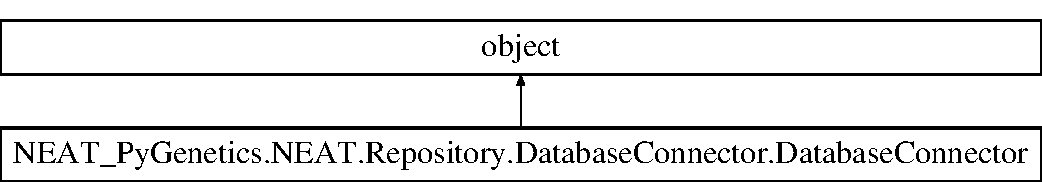
\includegraphics[height=2.000000cm]{class_n_e_a_t___py_genetics_1_1_n_e_a_t_1_1_repository_1_1_database_connector_1_1_database_connector}
\end{center}
\end{figure}
\subsection*{Public Member Functions}
\begin{DoxyCompactItemize}
\item 
def {\bfseries \+\_\+\+\_\+init\+\_\+\+\_\+}\hypertarget{class_n_e_a_t___py_genetics_1_1_n_e_a_t_1_1_repository_1_1_database_connector_1_1_database_connector_a57537c32ba05cb1800b4966a9b5ff97f}{}\label{class_n_e_a_t___py_genetics_1_1_n_e_a_t_1_1_repository_1_1_database_connector_1_1_database_connector_a57537c32ba05cb1800b4966a9b5ff97f}

\item 
def {\bfseries get\+\_\+collection}\hypertarget{class_n_e_a_t___py_genetics_1_1_n_e_a_t_1_1_repository_1_1_database_connector_1_1_database_connector_a0531d203c5909eb70a1f328f1ee87e46}{}\label{class_n_e_a_t___py_genetics_1_1_n_e_a_t_1_1_repository_1_1_database_connector_1_1_database_connector_a0531d203c5909eb70a1f328f1ee87e46}

\item 
def {\bfseries insert\+\_\+one}\hypertarget{class_n_e_a_t___py_genetics_1_1_n_e_a_t_1_1_repository_1_1_database_connector_1_1_database_connector_a1c8d38690f25313e30e339bb449e2afc}{}\label{class_n_e_a_t___py_genetics_1_1_n_e_a_t_1_1_repository_1_1_database_connector_1_1_database_connector_a1c8d38690f25313e30e339bb449e2afc}

\item 
def {\bfseries insert\+\_\+many}\hypertarget{class_n_e_a_t___py_genetics_1_1_n_e_a_t_1_1_repository_1_1_database_connector_1_1_database_connector_acaa494840a4f5c9ed45efc87a7b3c9e3}{}\label{class_n_e_a_t___py_genetics_1_1_n_e_a_t_1_1_repository_1_1_database_connector_1_1_database_connector_acaa494840a4f5c9ed45efc87a7b3c9e3}

\item 
def {\bfseries find\+\_\+one}\hypertarget{class_n_e_a_t___py_genetics_1_1_n_e_a_t_1_1_repository_1_1_database_connector_1_1_database_connector_a01ed6b2bbdf7e49c3b12260e8f716df0}{}\label{class_n_e_a_t___py_genetics_1_1_n_e_a_t_1_1_repository_1_1_database_connector_1_1_database_connector_a01ed6b2bbdf7e49c3b12260e8f716df0}

\item 
def {\bfseries find\+\_\+one\+\_\+by\+\_\+id}\hypertarget{class_n_e_a_t___py_genetics_1_1_n_e_a_t_1_1_repository_1_1_database_connector_1_1_database_connector_ab84e5e82fb7f4ef7e63d1a463f931d0b}{}\label{class_n_e_a_t___py_genetics_1_1_n_e_a_t_1_1_repository_1_1_database_connector_1_1_database_connector_ab84e5e82fb7f4ef7e63d1a463f931d0b}

\item 
def {\bfseries find\+\_\+many}\hypertarget{class_n_e_a_t___py_genetics_1_1_n_e_a_t_1_1_repository_1_1_database_connector_1_1_database_connector_a4f488daecf67131f0a138fbe02d75ad1}{}\label{class_n_e_a_t___py_genetics_1_1_n_e_a_t_1_1_repository_1_1_database_connector_1_1_database_connector_a4f488daecf67131f0a138fbe02d75ad1}

\item 
def {\bfseries update\+\_\+one}\hypertarget{class_n_e_a_t___py_genetics_1_1_n_e_a_t_1_1_repository_1_1_database_connector_1_1_database_connector_a44ca72a0a552c2c68bb6818e3902548e}{}\label{class_n_e_a_t___py_genetics_1_1_n_e_a_t_1_1_repository_1_1_database_connector_1_1_database_connector_a44ca72a0a552c2c68bb6818e3902548e}

\item 
def {\bfseries update\+\_\+many}\hypertarget{class_n_e_a_t___py_genetics_1_1_n_e_a_t_1_1_repository_1_1_database_connector_1_1_database_connector_a1181a46de443df2c30f65c5585984eab}{}\label{class_n_e_a_t___py_genetics_1_1_n_e_a_t_1_1_repository_1_1_database_connector_1_1_database_connector_a1181a46de443df2c30f65c5585984eab}

\item 
def {\bfseries remove\+\_\+one}\hypertarget{class_n_e_a_t___py_genetics_1_1_n_e_a_t_1_1_repository_1_1_database_connector_1_1_database_connector_a562cd964aa44d7e6051d1436acf047ba}{}\label{class_n_e_a_t___py_genetics_1_1_n_e_a_t_1_1_repository_1_1_database_connector_1_1_database_connector_a562cd964aa44d7e6051d1436acf047ba}

\item 
def {\bfseries remove\+\_\+many}\hypertarget{class_n_e_a_t___py_genetics_1_1_n_e_a_t_1_1_repository_1_1_database_connector_1_1_database_connector_ab576f403333ef9dc793d328bd04c41b6}{}\label{class_n_e_a_t___py_genetics_1_1_n_e_a_t_1_1_repository_1_1_database_connector_1_1_database_connector_ab576f403333ef9dc793d328bd04c41b6}

\end{DoxyCompactItemize}
\subsection*{Static Public Attributes}
\begin{DoxyCompactItemize}
\item 
{\bfseries result\+\_\+ids}\hypertarget{class_n_e_a_t___py_genetics_1_1_n_e_a_t_1_1_repository_1_1_database_connector_1_1_database_connector_ae6a5bd1fe8b17e6f4daeb34016befacc}{}\label{class_n_e_a_t___py_genetics_1_1_n_e_a_t_1_1_repository_1_1_database_connector_1_1_database_connector_ae6a5bd1fe8b17e6f4daeb34016befacc}

\item 
{\bfseries i}\hypertarget{class_n_e_a_t___py_genetics_1_1_n_e_a_t_1_1_repository_1_1_database_connector_1_1_database_connector_aa64c3cdec4a68d8b9cb70eff5fc65da1}{}\label{class_n_e_a_t___py_genetics_1_1_n_e_a_t_1_1_repository_1_1_database_connector_1_1_database_connector_aa64c3cdec4a68d8b9cb70eff5fc65da1}

\item 
{\bfseries result}\hypertarget{class_n_e_a_t___py_genetics_1_1_n_e_a_t_1_1_repository_1_1_database_connector_1_1_database_connector_ac4e5c7484ac4c90604a438b88250f4cc}{}\label{class_n_e_a_t___py_genetics_1_1_n_e_a_t_1_1_repository_1_1_database_connector_1_1_database_connector_ac4e5c7484ac4c90604a438b88250f4cc}

\end{DoxyCompactItemize}


\subsection{Detailed Description}


Definition at line 9 of file Database\+Connector.\+py.



The documentation for this class was generated from the following file\+:\begin{DoxyCompactItemize}
\item 
N\+E\+A\+T/\+Repository/Database\+Connector.\+py\end{DoxyCompactItemize}

\hypertarget{class_n_e_a_t___py_genetics_1_1_n_e_a_t_1_1_tests_1_1_repository_tests_1_1test__database_connector_1_1_database_connector_test}{}\section{N\+E\+A\+T\+\_\+\+Py\+Genetics.\+N\+E\+A\+T.\+Tests.\+Repository\+Tests.\+test\+\_\+database\+Connector.\+Database\+Connector\+Test Class Reference}
\label{class_n_e_a_t___py_genetics_1_1_n_e_a_t_1_1_tests_1_1_repository_tests_1_1test__database_connector_1_1_database_connector_test}\index{N\+E\+A\+T\+\_\+\+Py\+Genetics.\+N\+E\+A\+T.\+Tests.\+Repository\+Tests.\+test\+\_\+database\+Connector.\+Database\+Connector\+Test@{N\+E\+A\+T\+\_\+\+Py\+Genetics.\+N\+E\+A\+T.\+Tests.\+Repository\+Tests.\+test\+\_\+database\+Connector.\+Database\+Connector\+Test}}
Inheritance diagram for N\+E\+A\+T\+\_\+\+Py\+Genetics.\+N\+E\+A\+T.\+Tests.\+Repository\+Tests.\+test\+\_\+database\+Connector.\+Database\+Connector\+Test\+:\begin{figure}[H]
\begin{center}
\leavevmode
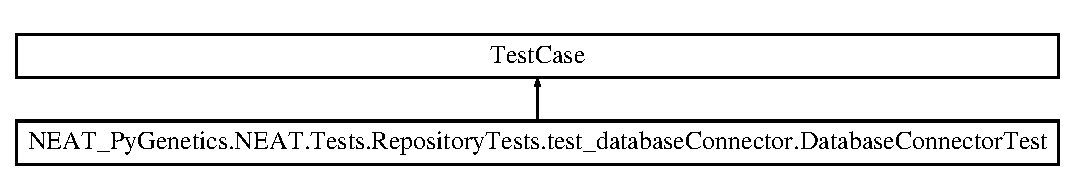
\includegraphics[height=1.978799cm]{class_n_e_a_t___py_genetics_1_1_n_e_a_t_1_1_tests_1_1_repository_tests_1_1test__database_connector_1_1_database_connector_test}
\end{center}
\end{figure}
\subsection*{Public Member Functions}
\begin{DoxyCompactItemize}
\item 
def {\bfseries set\+Up} (self)\hypertarget{class_n_e_a_t___py_genetics_1_1_n_e_a_t_1_1_tests_1_1_repository_tests_1_1test__database_connector_1_1_database_connector_test_a91d61974260986974a20508255b4ac15}{}\label{class_n_e_a_t___py_genetics_1_1_n_e_a_t_1_1_tests_1_1_repository_tests_1_1test__database_connector_1_1_database_connector_test_a91d61974260986974a20508255b4ac15}

\item 
def {\bfseries test\+\_\+get\+Collection} (self)\hypertarget{class_n_e_a_t___py_genetics_1_1_n_e_a_t_1_1_tests_1_1_repository_tests_1_1test__database_connector_1_1_database_connector_test_af5c978077be86b490cb1fc5ddd45b8a6}{}\label{class_n_e_a_t___py_genetics_1_1_n_e_a_t_1_1_tests_1_1_repository_tests_1_1test__database_connector_1_1_database_connector_test_af5c978077be86b490cb1fc5ddd45b8a6}

\item 
def {\bfseries test\+\_\+insert\+One} (self)\hypertarget{class_n_e_a_t___py_genetics_1_1_n_e_a_t_1_1_tests_1_1_repository_tests_1_1test__database_connector_1_1_database_connector_test_a0cb8fdc59961c49884fc3eedbc7f3dd5}{}\label{class_n_e_a_t___py_genetics_1_1_n_e_a_t_1_1_tests_1_1_repository_tests_1_1test__database_connector_1_1_database_connector_test_a0cb8fdc59961c49884fc3eedbc7f3dd5}

\item 
def {\bfseries test\+\_\+insert\+Many} (self)\hypertarget{class_n_e_a_t___py_genetics_1_1_n_e_a_t_1_1_tests_1_1_repository_tests_1_1test__database_connector_1_1_database_connector_test_a98a79c5760b6dc3f2157af53fe6001a3}{}\label{class_n_e_a_t___py_genetics_1_1_n_e_a_t_1_1_tests_1_1_repository_tests_1_1test__database_connector_1_1_database_connector_test_a98a79c5760b6dc3f2157af53fe6001a3}

\item 
def {\bfseries test\+\_\+find\+One} (self)\hypertarget{class_n_e_a_t___py_genetics_1_1_n_e_a_t_1_1_tests_1_1_repository_tests_1_1test__database_connector_1_1_database_connector_test_a7ea0327574316e92b1b866b823639e09}{}\label{class_n_e_a_t___py_genetics_1_1_n_e_a_t_1_1_tests_1_1_repository_tests_1_1test__database_connector_1_1_database_connector_test_a7ea0327574316e92b1b866b823639e09}

\item 
def {\bfseries test\+\_\+find\+One\+By\+Id} (self)\hypertarget{class_n_e_a_t___py_genetics_1_1_n_e_a_t_1_1_tests_1_1_repository_tests_1_1test__database_connector_1_1_database_connector_test_a903ee479fb3ef1432cdf9fd4e1464e5e}{}\label{class_n_e_a_t___py_genetics_1_1_n_e_a_t_1_1_tests_1_1_repository_tests_1_1test__database_connector_1_1_database_connector_test_a903ee479fb3ef1432cdf9fd4e1464e5e}

\item 
def {\bfseries test\+\_\+find\+Many} (self)\hypertarget{class_n_e_a_t___py_genetics_1_1_n_e_a_t_1_1_tests_1_1_repository_tests_1_1test__database_connector_1_1_database_connector_test_a08ec69775b40a8081e3e09b85ff35969}{}\label{class_n_e_a_t___py_genetics_1_1_n_e_a_t_1_1_tests_1_1_repository_tests_1_1test__database_connector_1_1_database_connector_test_a08ec69775b40a8081e3e09b85ff35969}

\item 
def {\bfseries test\+\_\+update\+One} (self)\hypertarget{class_n_e_a_t___py_genetics_1_1_n_e_a_t_1_1_tests_1_1_repository_tests_1_1test__database_connector_1_1_database_connector_test_a2b589e245c56dad59a11844c5c273c2f}{}\label{class_n_e_a_t___py_genetics_1_1_n_e_a_t_1_1_tests_1_1_repository_tests_1_1test__database_connector_1_1_database_connector_test_a2b589e245c56dad59a11844c5c273c2f}

\item 
def {\bfseries test\+\_\+update\+Many\+Fail} (self)\hypertarget{class_n_e_a_t___py_genetics_1_1_n_e_a_t_1_1_tests_1_1_repository_tests_1_1test__database_connector_1_1_database_connector_test_a9b491c21b224c52ae6f7309fb49eedf5}{}\label{class_n_e_a_t___py_genetics_1_1_n_e_a_t_1_1_tests_1_1_repository_tests_1_1test__database_connector_1_1_database_connector_test_a9b491c21b224c52ae6f7309fb49eedf5}

\item 
def {\bfseries test\+\_\+update\+Many} (self)\hypertarget{class_n_e_a_t___py_genetics_1_1_n_e_a_t_1_1_tests_1_1_repository_tests_1_1test__database_connector_1_1_database_connector_test_a515f4b176113719b0198bfa91647c63e}{}\label{class_n_e_a_t___py_genetics_1_1_n_e_a_t_1_1_tests_1_1_repository_tests_1_1test__database_connector_1_1_database_connector_test_a515f4b176113719b0198bfa91647c63e}

\item 
def {\bfseries test\+\_\+remove\+One} (self)\hypertarget{class_n_e_a_t___py_genetics_1_1_n_e_a_t_1_1_tests_1_1_repository_tests_1_1test__database_connector_1_1_database_connector_test_a14bc136f4338528fb46c51925d89c7ac}{}\label{class_n_e_a_t___py_genetics_1_1_n_e_a_t_1_1_tests_1_1_repository_tests_1_1test__database_connector_1_1_database_connector_test_a14bc136f4338528fb46c51925d89c7ac}

\item 
def {\bfseries test\+\_\+remove\+Many} (self)\hypertarget{class_n_e_a_t___py_genetics_1_1_n_e_a_t_1_1_tests_1_1_repository_tests_1_1test__database_connector_1_1_database_connector_test_a86194fa471e1217076ee3a080790b82d}{}\label{class_n_e_a_t___py_genetics_1_1_n_e_a_t_1_1_tests_1_1_repository_tests_1_1test__database_connector_1_1_database_connector_test_a86194fa471e1217076ee3a080790b82d}

\end{DoxyCompactItemize}
\subsection*{Public Attributes}
\begin{DoxyCompactItemize}
\item 
{\bfseries db}\hypertarget{class_n_e_a_t___py_genetics_1_1_n_e_a_t_1_1_tests_1_1_repository_tests_1_1test__database_connector_1_1_database_connector_test_a9115740100acd95dbd3a72371acfe681}{}\label{class_n_e_a_t___py_genetics_1_1_n_e_a_t_1_1_tests_1_1_repository_tests_1_1test__database_connector_1_1_database_connector_test_a9115740100acd95dbd3a72371acfe681}

\item 
{\bfseries collection}\hypertarget{class_n_e_a_t___py_genetics_1_1_n_e_a_t_1_1_tests_1_1_repository_tests_1_1test__database_connector_1_1_database_connector_test_aca0cb75295bf0c9964cceef08fa98b7b}{}\label{class_n_e_a_t___py_genetics_1_1_n_e_a_t_1_1_tests_1_1_repository_tests_1_1test__database_connector_1_1_database_connector_test_aca0cb75295bf0c9964cceef08fa98b7b}

\item 
{\bfseries database\+\_\+connector}\hypertarget{class_n_e_a_t___py_genetics_1_1_n_e_a_t_1_1_tests_1_1_repository_tests_1_1test__database_connector_1_1_database_connector_test_aafa6c5991087684c1187c529c8f76682}{}\label{class_n_e_a_t___py_genetics_1_1_n_e_a_t_1_1_tests_1_1_repository_tests_1_1test__database_connector_1_1_database_connector_test_aafa6c5991087684c1187c529c8f76682}

\end{DoxyCompactItemize}


\subsection{Detailed Description}


Definition at line 8 of file test\+\_\+database\+Connector.\+py.



The documentation for this class was generated from the following file\+:\begin{DoxyCompactItemize}
\item 
N\+E\+A\+T/\+Tests/\+Repository\+Tests/test\+\_\+database\+Connector.\+py\end{DoxyCompactItemize}

\hypertarget{class_n_e_a_t___py_genetics_1_1_n_e_a_t_1_1_decisions_1_1_decision_maker_1_1_decision_maker}{}\section{N\+E\+A\+T\+\_\+\+Py\+Genetics.\+N\+E\+A\+T.\+Decisions.\+Decision\+Maker.\+Decision\+Maker Class Reference}
\label{class_n_e_a_t___py_genetics_1_1_n_e_a_t_1_1_decisions_1_1_decision_maker_1_1_decision_maker}\index{N\+E\+A\+T\+\_\+\+Py\+Genetics.\+N\+E\+A\+T.\+Decisions.\+Decision\+Maker.\+Decision\+Maker@{N\+E\+A\+T\+\_\+\+Py\+Genetics.\+N\+E\+A\+T.\+Decisions.\+Decision\+Maker.\+Decision\+Maker}}
Inheritance diagram for N\+E\+A\+T\+\_\+\+Py\+Genetics.\+N\+E\+A\+T.\+Decisions.\+Decision\+Maker.\+Decision\+Maker\+:\begin{figure}[H]
\begin{center}
\leavevmode
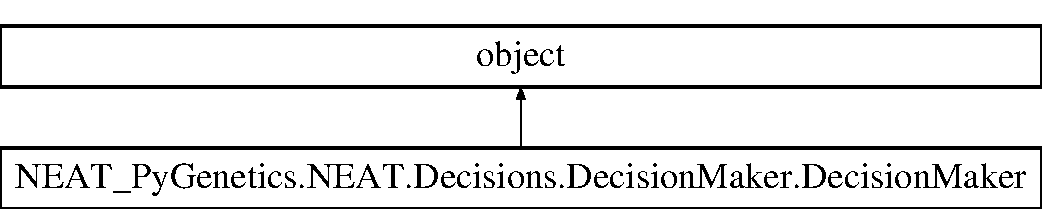
\includegraphics[height=2.000000cm]{class_n_e_a_t___py_genetics_1_1_n_e_a_t_1_1_decisions_1_1_decision_maker_1_1_decision_maker}
\end{center}
\end{figure}
\subsection*{Public Member Functions}
\begin{DoxyCompactItemize}
\item 
def {\bfseries \+\_\+\+\_\+init\+\_\+\+\_\+} (self, decision\+\_\+making\+\_\+parameters)\hypertarget{class_n_e_a_t___py_genetics_1_1_n_e_a_t_1_1_decisions_1_1_decision_maker_1_1_decision_maker_a7691e28dc58fcd50858edcbf206c5bd9}{}\label{class_n_e_a_t___py_genetics_1_1_n_e_a_t_1_1_decisions_1_1_decision_maker_1_1_decision_maker_a7691e28dc58fcd50858edcbf206c5bd9}

\item 
def {\bfseries advance\+\_\+time} (self)\hypertarget{class_n_e_a_t___py_genetics_1_1_n_e_a_t_1_1_decisions_1_1_decision_maker_1_1_decision_maker_aee1f2396d8dfe5fd8e47f86bf6ffdb84}{}\label{class_n_e_a_t___py_genetics_1_1_n_e_a_t_1_1_decisions_1_1_decision_maker_1_1_decision_maker_aee1f2396d8dfe5fd8e47f86bf6ffdb84}

\item 
def {\bfseries reset\+\_\+time} (self)\hypertarget{class_n_e_a_t___py_genetics_1_1_n_e_a_t_1_1_decisions_1_1_decision_maker_1_1_decision_maker_a18ac18ed4d2954404ea8b58e45b2f176}{}\label{class_n_e_a_t___py_genetics_1_1_n_e_a_t_1_1_decisions_1_1_decision_maker_1_1_decision_maker_a18ac18ed4d2954404ea8b58e45b2f176}

\item 
def {\bfseries mutation\+\_\+percentage} (self)\hypertarget{class_n_e_a_t___py_genetics_1_1_n_e_a_t_1_1_decisions_1_1_decision_maker_1_1_decision_maker_ac441f750aa9b1853744bf49b5e195249}{}\label{class_n_e_a_t___py_genetics_1_1_n_e_a_t_1_1_decisions_1_1_decision_maker_1_1_decision_maker_ac441f750aa9b1853744bf49b5e195249}

\item 
def {\bfseries inter\+\_\+cluster\+\_\+breeding\+\_\+time} (self)\hypertarget{class_n_e_a_t___py_genetics_1_1_n_e_a_t_1_1_decisions_1_1_decision_maker_1_1_decision_maker_ab7cf16b4c29f75b24dec3c6f887b1cea}{}\label{class_n_e_a_t___py_genetics_1_1_n_e_a_t_1_1_decisions_1_1_decision_maker_1_1_decision_maker_ab7cf16b4c29f75b24dec3c6f887b1cea}

\end{DoxyCompactItemize}


\subsection{Detailed Description}


Definition at line 7 of file Decision\+Maker.\+py.



The documentation for this class was generated from the following file\+:\begin{DoxyCompactItemize}
\item 
N\+E\+A\+T/\+Decisions/Decision\+Maker.\+py\end{DoxyCompactItemize}

\hypertarget{class_n_e_a_t___py_genetics_1_1_n_e_a_t_1_1_director_1_1_director_1_1_director}{}\section{N\+E\+A\+T\+\_\+\+Py\+Genetics.\+N\+E\+A\+T.\+Director.\+Director.\+Director Class Reference}
\label{class_n_e_a_t___py_genetics_1_1_n_e_a_t_1_1_director_1_1_director_1_1_director}\index{N\+E\+A\+T\+\_\+\+Py\+Genetics.\+N\+E\+A\+T.\+Director.\+Director.\+Director@{N\+E\+A\+T\+\_\+\+Py\+Genetics.\+N\+E\+A\+T.\+Director.\+Director.\+Director}}
Inheritance diagram for N\+E\+A\+T\+\_\+\+Py\+Genetics.\+N\+E\+A\+T.\+Director.\+Director.\+Director\+:\begin{figure}[H]
\begin{center}
\leavevmode
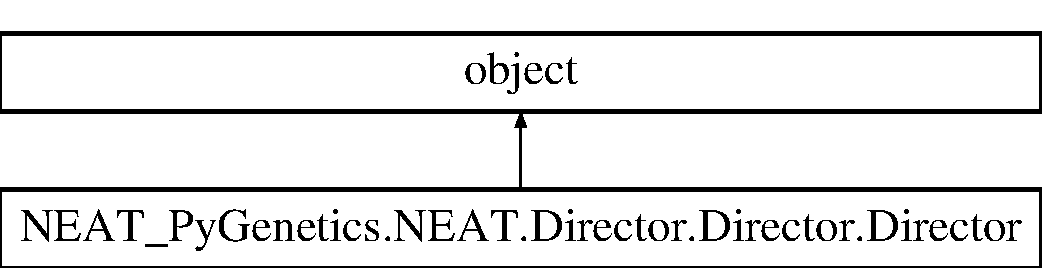
\includegraphics[height=2.000000cm]{class_n_e_a_t___py_genetics_1_1_n_e_a_t_1_1_director_1_1_director_1_1_director}
\end{center}
\end{figure}
\subsection*{Public Member Functions}
\begin{DoxyCompactItemize}
\item 
def {\bfseries run} (self)\hypertarget{class_n_e_a_t___py_genetics_1_1_n_e_a_t_1_1_director_1_1_director_1_1_director_a2e4d16b66d8b60ec696d3c734a7e5833}{}\label{class_n_e_a_t___py_genetics_1_1_n_e_a_t_1_1_director_1_1_director_1_1_director_a2e4d16b66d8b60ec696d3c734a7e5833}

\end{DoxyCompactItemize}


\subsection{Detailed Description}


Definition at line 1 of file Director.\+py.



The documentation for this class was generated from the following file\+:\begin{DoxyCompactItemize}
\item 
N\+E\+A\+T/\+Director/Director.\+py\end{DoxyCompactItemize}

\hypertarget{class_n_e_a_t___py_genetics_1_1_n_e_a_t_1_1_repository_1_1_gene_repository_1_1_gene_repository}{}\section{N\+E\+A\+T\+\_\+\+Py\+Genetics.\+N\+E\+A\+T.\+Repository.\+Gene\+Repository.\+Gene\+Repository Class Reference}
\label{class_n_e_a_t___py_genetics_1_1_n_e_a_t_1_1_repository_1_1_gene_repository_1_1_gene_repository}\index{N\+E\+A\+T\+\_\+\+Py\+Genetics.\+N\+E\+A\+T.\+Repository.\+Gene\+Repository.\+Gene\+Repository@{N\+E\+A\+T\+\_\+\+Py\+Genetics.\+N\+E\+A\+T.\+Repository.\+Gene\+Repository.\+Gene\+Repository}}
Inheritance diagram for N\+E\+A\+T\+\_\+\+Py\+Genetics.\+N\+E\+A\+T.\+Repository.\+Gene\+Repository.\+Gene\+Repository\+:\begin{figure}[H]
\begin{center}
\leavevmode
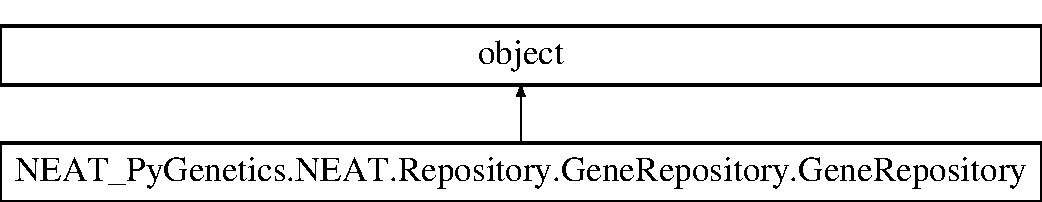
\includegraphics[height=2.000000cm]{class_n_e_a_t___py_genetics_1_1_n_e_a_t_1_1_repository_1_1_gene_repository_1_1_gene_repository}
\end{center}
\end{figure}
\subsection*{Public Member Functions}
\begin{DoxyCompactItemize}
\item 
def {\bfseries \+\_\+\+\_\+init\+\_\+\+\_\+}\hypertarget{class_n_e_a_t___py_genetics_1_1_n_e_a_t_1_1_repository_1_1_gene_repository_1_1_gene_repository_a47867f001b69fb1af342bd56077eb2d1}{}\label{class_n_e_a_t___py_genetics_1_1_n_e_a_t_1_1_repository_1_1_gene_repository_1_1_gene_repository_a47867f001b69fb1af342bd56077eb2d1}

\item 
def {\bfseries get\+\_\+gene\+\_\+id\+\_\+for\+\_\+endpoints} (self, head\+\_\+node\+\_\+id, tail\+\_\+node\+\_\+id)\hypertarget{class_n_e_a_t___py_genetics_1_1_n_e_a_t_1_1_repository_1_1_gene_repository_1_1_gene_repository_acf117ca8d8fb85263ab1e419e795bc3f}{}\label{class_n_e_a_t___py_genetics_1_1_n_e_a_t_1_1_repository_1_1_gene_repository_1_1_gene_repository_acf117ca8d8fb85263ab1e419e795bc3f}

\item 
def {\bfseries find\+\_\+connecting\+\_\+nodes} (self, head\+\_\+node\+\_\+id, tail\+\_\+node\+\_\+id)\hypertarget{class_n_e_a_t___py_genetics_1_1_n_e_a_t_1_1_repository_1_1_gene_repository_1_1_gene_repository_a12b448287c1e00d71325a0f4f5191b0b}{}\label{class_n_e_a_t___py_genetics_1_1_n_e_a_t_1_1_repository_1_1_gene_repository_1_1_gene_repository_a12b448287c1e00d71325a0f4f5191b0b}

\item 
def {\bfseries get\+\_\+next\+\_\+node\+\_\+label} (self)\hypertarget{class_n_e_a_t___py_genetics_1_1_n_e_a_t_1_1_repository_1_1_gene_repository_1_1_gene_repository_a1cf66c6d6fbb68a38a5915ccfbab77cb}{}\label{class_n_e_a_t___py_genetics_1_1_n_e_a_t_1_1_repository_1_1_gene_repository_1_1_gene_repository_a1cf66c6d6fbb68a38a5915ccfbab77cb}

\item 
def {\bfseries get\+\_\+node\+\_\+labels\+\_\+by\+\_\+gene\+\_\+id} (self, gene\+\_\+id)\hypertarget{class_n_e_a_t___py_genetics_1_1_n_e_a_t_1_1_repository_1_1_gene_repository_1_1_gene_repository_a135cdf881aca932199a40ace71aa88e2}{}\label{class_n_e_a_t___py_genetics_1_1_n_e_a_t_1_1_repository_1_1_gene_repository_1_1_gene_repository_a135cdf881aca932199a40ace71aa88e2}

\end{DoxyCompactItemize}


\subsection{Detailed Description}


Definition at line 5 of file Gene\+Repository.\+py.



The documentation for this class was generated from the following file\+:\begin{DoxyCompactItemize}
\item 
N\+E\+A\+T/\+Repository/Gene\+Repository.\+py\end{DoxyCompactItemize}

\hypertarget{class_n_e_a_t___py_genetics_1_1_n_e_a_t_1_1_analyst_1_1_genome_analyst_1_1_genome_analyst}{}\section{N\+E\+A\+T\+\_\+\+Py\+Genetics.\+N\+E\+A\+T.\+Analyst.\+Genome\+Analyst.\+Genome\+Analyst Class Reference}
\label{class_n_e_a_t___py_genetics_1_1_n_e_a_t_1_1_analyst_1_1_genome_analyst_1_1_genome_analyst}\index{N\+E\+A\+T\+\_\+\+Py\+Genetics.\+N\+E\+A\+T.\+Analyst.\+Genome\+Analyst.\+Genome\+Analyst@{N\+E\+A\+T\+\_\+\+Py\+Genetics.\+N\+E\+A\+T.\+Analyst.\+Genome\+Analyst.\+Genome\+Analyst}}
Inheritance diagram for N\+E\+A\+T\+\_\+\+Py\+Genetics.\+N\+E\+A\+T.\+Analyst.\+Genome\+Analyst.\+Genome\+Analyst\+:\begin{figure}[H]
\begin{center}
\leavevmode
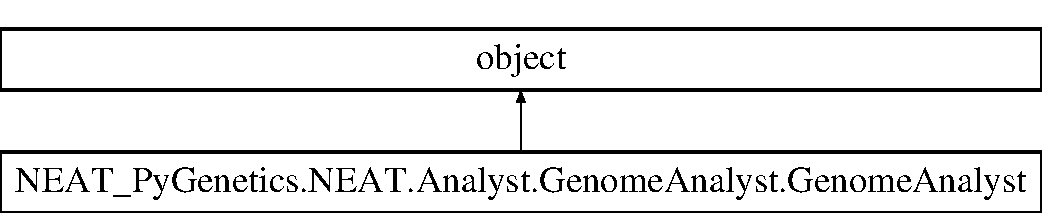
\includegraphics[height=2.000000cm]{class_n_e_a_t___py_genetics_1_1_n_e_a_t_1_1_analyst_1_1_genome_analyst_1_1_genome_analyst}
\end{center}
\end{figure}
\subsection*{Public Member Functions}
\begin{DoxyCompactItemize}
\item 
def \hyperlink{class_n_e_a_t___py_genetics_1_1_n_e_a_t_1_1_analyst_1_1_genome_analyst_1_1_genome_analyst_a2b9e3334de517a0555177ee6bcc0ac04}{\+\_\+\+\_\+init\+\_\+\+\_\+} (self)
\item 
def {\bfseries analyze}\hypertarget{class_n_e_a_t___py_genetics_1_1_n_e_a_t_1_1_analyst_1_1_genome_analyst_1_1_genome_analyst_afdd3b4e6b0b8275dd62677b8d5a18933}{}\label{class_n_e_a_t___py_genetics_1_1_n_e_a_t_1_1_analyst_1_1_genome_analyst_1_1_genome_analyst_afdd3b4e6b0b8275dd62677b8d5a18933}

\end{DoxyCompactItemize}
\subsection*{Static Public Attributes}
\begin{DoxyCompactItemize}
\item 
{\bfseries topologically\+\_\+sorted\+\_\+nodes}\hypertarget{class_n_e_a_t___py_genetics_1_1_n_e_a_t_1_1_analyst_1_1_genome_analyst_1_1_genome_analyst_a61333814f998f2c80d271f3ebc92d198}{}\label{class_n_e_a_t___py_genetics_1_1_n_e_a_t_1_1_analyst_1_1_genome_analyst_1_1_genome_analyst_a61333814f998f2c80d271f3ebc92d198}

\item 
{\bfseries cycle\+\_\+edges}\hypertarget{class_n_e_a_t___py_genetics_1_1_n_e_a_t_1_1_analyst_1_1_genome_analyst_1_1_genome_analyst_a5453383e771c7f655739ee80508a8b08}{}\label{class_n_e_a_t___py_genetics_1_1_n_e_a_t_1_1_analyst_1_1_genome_analyst_1_1_genome_analyst_a5453383e771c7f655739ee80508a8b08}

\item 
{\bfseries topologically\+\_\+sorted\+\_\+cycle\+\_\+nodes}\hypertarget{class_n_e_a_t___py_genetics_1_1_n_e_a_t_1_1_analyst_1_1_genome_analyst_1_1_genome_analyst_adee62c855c0445f8b5c4032ceaf1217d}{}\label{class_n_e_a_t___py_genetics_1_1_n_e_a_t_1_1_analyst_1_1_genome_analyst_1_1_genome_analyst_adee62c855c0445f8b5c4032ceaf1217d}

\end{DoxyCompactItemize}


\subsection{Detailed Description}


Definition at line 8 of file Genome\+Analyst.\+py.



\subsection{Constructor \& Destructor Documentation}
\index{N\+E\+A\+T\+\_\+\+Py\+Genetics\+::\+N\+E\+A\+T\+::\+Analyst\+::\+Genome\+Analyst\+::\+Genome\+Analyst@{N\+E\+A\+T\+\_\+\+Py\+Genetics\+::\+N\+E\+A\+T\+::\+Analyst\+::\+Genome\+Analyst\+::\+Genome\+Analyst}!\+\_\+\+\_\+init\+\_\+\+\_\+@{\+\_\+\+\_\+init\+\_\+\+\_\+}}
\index{\+\_\+\+\_\+init\+\_\+\+\_\+@{\+\_\+\+\_\+init\+\_\+\+\_\+}!N\+E\+A\+T\+\_\+\+Py\+Genetics\+::\+N\+E\+A\+T\+::\+Analyst\+::\+Genome\+Analyst\+::\+Genome\+Analyst@{N\+E\+A\+T\+\_\+\+Py\+Genetics\+::\+N\+E\+A\+T\+::\+Analyst\+::\+Genome\+Analyst\+::\+Genome\+Analyst}}
\subsubsection[{\texorpdfstring{\+\_\+\+\_\+init\+\_\+\+\_\+(self)}{__init__(self)}}]{\setlength{\rightskip}{0pt plus 5cm}def N\+E\+A\+T\+\_\+\+Py\+Genetics.\+N\+E\+A\+T.\+Analyst.\+Genome\+Analyst.\+Genome\+Analyst.\+\_\+\+\_\+init\+\_\+\+\_\+ (
\begin{DoxyParamCaption}
\item[{}]{self}
\end{DoxyParamCaption}
)}\hypertarget{class_n_e_a_t___py_genetics_1_1_n_e_a_t_1_1_analyst_1_1_genome_analyst_1_1_genome_analyst_a2b9e3334de517a0555177ee6bcc0ac04}{}\label{class_n_e_a_t___py_genetics_1_1_n_e_a_t_1_1_analyst_1_1_genome_analyst_1_1_genome_analyst_a2b9e3334de517a0555177ee6bcc0ac04}
\begin{DoxyVerb}_node_visited:
  _node_visited[i] = 0 => node with id i was not visited yet
  _node_visited[i] = 1 => node with id i was visited
:return:
\end{DoxyVerb}
 

Definition at line 9 of file Genome\+Analyst.\+py.



The documentation for this class was generated from the following file\+:\begin{DoxyCompactItemize}
\item 
N\+E\+A\+T/\+Analyst/Genome\+Analyst.\+py\end{DoxyCompactItemize}

\hypertarget{class_n_e_a_t___py_genetics_1_1_n_e_a_t_1_1_analyst_1_1_genome_clusterer_1_1_genome_clusterer}{}\section{N\+E\+A\+T\+\_\+\+Py\+Genetics.\+N\+E\+A\+T.\+Analyst.\+Genome\+Clusterer.\+Genome\+Clusterer Class Reference}
\label{class_n_e_a_t___py_genetics_1_1_n_e_a_t_1_1_analyst_1_1_genome_clusterer_1_1_genome_clusterer}\index{N\+E\+A\+T\+\_\+\+Py\+Genetics.\+N\+E\+A\+T.\+Analyst.\+Genome\+Clusterer.\+Genome\+Clusterer@{N\+E\+A\+T\+\_\+\+Py\+Genetics.\+N\+E\+A\+T.\+Analyst.\+Genome\+Clusterer.\+Genome\+Clusterer}}
Inheritance diagram for N\+E\+A\+T\+\_\+\+Py\+Genetics.\+N\+E\+A\+T.\+Analyst.\+Genome\+Clusterer.\+Genome\+Clusterer\+:\begin{figure}[H]
\begin{center}
\leavevmode
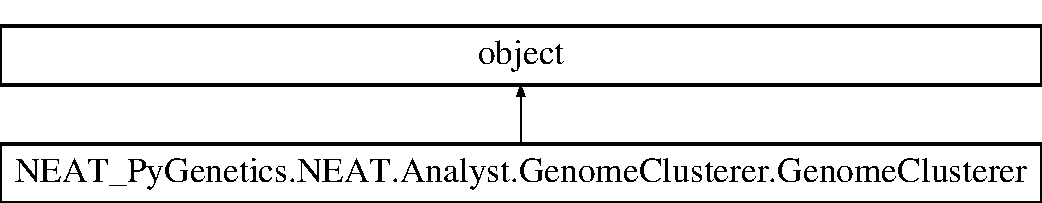
\includegraphics[height=2.000000cm]{class_n_e_a_t___py_genetics_1_1_n_e_a_t_1_1_analyst_1_1_genome_clusterer_1_1_genome_clusterer}
\end{center}
\end{figure}
\subsection*{Public Member Functions}
\begin{DoxyCompactItemize}
\item 
def {\bfseries \+\_\+\+\_\+init\+\_\+\+\_\+}\hypertarget{class_n_e_a_t___py_genetics_1_1_n_e_a_t_1_1_analyst_1_1_genome_clusterer_1_1_genome_clusterer_a2f18f1f814c59bc18bc896c67331db10}{}\label{class_n_e_a_t___py_genetics_1_1_n_e_a_t_1_1_analyst_1_1_genome_clusterer_1_1_genome_clusterer_a2f18f1f814c59bc18bc896c67331db10}

\item 
def {\bfseries cluster\+\_\+genomes}\hypertarget{class_n_e_a_t___py_genetics_1_1_n_e_a_t_1_1_analyst_1_1_genome_clusterer_1_1_genome_clusterer_a3cb27bd4e57fbae51f5638bf252d7d19}{}\label{class_n_e_a_t___py_genetics_1_1_n_e_a_t_1_1_analyst_1_1_genome_clusterer_1_1_genome_clusterer_a3cb27bd4e57fbae51f5638bf252d7d19}

\item 
def {\bfseries cluster\+\_\+genome}\hypertarget{class_n_e_a_t___py_genetics_1_1_n_e_a_t_1_1_analyst_1_1_genome_clusterer_1_1_genome_clusterer_a4b17098e6b96981aa7a00ffe3c3510c8}{}\label{class_n_e_a_t___py_genetics_1_1_n_e_a_t_1_1_analyst_1_1_genome_clusterer_1_1_genome_clusterer_a4b17098e6b96981aa7a00ffe3c3510c8}

\item 
def {\bfseries calculate\+\_\+delta}\hypertarget{class_n_e_a_t___py_genetics_1_1_n_e_a_t_1_1_analyst_1_1_genome_clusterer_1_1_genome_clusterer_a057cec399fba67f9f90c70ad9158ec5e}{}\label{class_n_e_a_t___py_genetics_1_1_n_e_a_t_1_1_analyst_1_1_genome_clusterer_1_1_genome_clusterer_a057cec399fba67f9f90c70ad9158ec5e}

\item 
def {\bfseries calculate\+\_\+cluster\+\_\+fitness}\hypertarget{class_n_e_a_t___py_genetics_1_1_n_e_a_t_1_1_analyst_1_1_genome_clusterer_1_1_genome_clusterer_a5dba985534b3de86bb03574e683749f6}{}\label{class_n_e_a_t___py_genetics_1_1_n_e_a_t_1_1_analyst_1_1_genome_clusterer_1_1_genome_clusterer_a5dba985534b3de86bb03574e683749f6}

\item 
def \hyperlink{class_n_e_a_t___py_genetics_1_1_n_e_a_t_1_1_analyst_1_1_genome_clusterer_1_1_genome_clusterer_a6bd0107d083dade08414c19ad9aaadaf}{calculate\+\_\+cluster\+\_\+offspring\+\_\+values} (self)
\end{DoxyCompactItemize}
\subsection*{Static Public Member Functions}
\begin{DoxyCompactItemize}
\item 
def {\bfseries calculate\+\_\+disjoint\+\_\+excess\+\_\+count}\hypertarget{class_n_e_a_t___py_genetics_1_1_n_e_a_t_1_1_analyst_1_1_genome_clusterer_1_1_genome_clusterer_a25f21d57d135bbf3b0f23bbfdef375e7}{}\label{class_n_e_a_t___py_genetics_1_1_n_e_a_t_1_1_analyst_1_1_genome_clusterer_1_1_genome_clusterer_a25f21d57d135bbf3b0f23bbfdef375e7}

\item 
def {\bfseries calculate\+\_\+average\+\_\+weight\+\_\+difference}\hypertarget{class_n_e_a_t___py_genetics_1_1_n_e_a_t_1_1_analyst_1_1_genome_clusterer_1_1_genome_clusterer_a748db217e8ce0c9f3e4302b00b4677e8}{}\label{class_n_e_a_t___py_genetics_1_1_n_e_a_t_1_1_analyst_1_1_genome_clusterer_1_1_genome_clusterer_a748db217e8ce0c9f3e4302b00b4677e8}

\end{DoxyCompactItemize}
\subsection*{Static Public Attributes}
\begin{DoxyCompactItemize}
\item 
{\bfseries genome\+\_\+repository}\hypertarget{class_n_e_a_t___py_genetics_1_1_n_e_a_t_1_1_analyst_1_1_genome_clusterer_1_1_genome_clusterer_af9623df2d784da3e4c186b729c63bb81}{}\label{class_n_e_a_t___py_genetics_1_1_n_e_a_t_1_1_analyst_1_1_genome_clusterer_1_1_genome_clusterer_af9623df2d784da3e4c186b729c63bb81}

\item 
{\bfseries cluster\+\_\+repository}\hypertarget{class_n_e_a_t___py_genetics_1_1_n_e_a_t_1_1_analyst_1_1_genome_clusterer_1_1_genome_clusterer_ab9332a669c7c28ee6d33806da38eee45}{}\label{class_n_e_a_t___py_genetics_1_1_n_e_a_t_1_1_analyst_1_1_genome_clusterer_1_1_genome_clusterer_ab9332a669c7c28ee6d33806da38eee45}

\item 
{\bfseries clustering\+\_\+parameters}\hypertarget{class_n_e_a_t___py_genetics_1_1_n_e_a_t_1_1_analyst_1_1_genome_clusterer_1_1_genome_clusterer_a23498ab192f633f9bada8709832b5fed}{}\label{class_n_e_a_t___py_genetics_1_1_n_e_a_t_1_1_analyst_1_1_genome_clusterer_1_1_genome_clusterer_a23498ab192f633f9bada8709832b5fed}

\item 
{\bfseries excess\+\_\+coefficient}\hypertarget{class_n_e_a_t___py_genetics_1_1_n_e_a_t_1_1_analyst_1_1_genome_clusterer_1_1_genome_clusterer_aefeaee4266e3fab9ff64f0b23fa08902}{}\label{class_n_e_a_t___py_genetics_1_1_n_e_a_t_1_1_analyst_1_1_genome_clusterer_1_1_genome_clusterer_aefeaee4266e3fab9ff64f0b23fa08902}

\item 
{\bfseries disjoint\+\_\+coefficient}\hypertarget{class_n_e_a_t___py_genetics_1_1_n_e_a_t_1_1_analyst_1_1_genome_clusterer_1_1_genome_clusterer_a2d3a31646312ae391f5805b5f5a7c0c5}{}\label{class_n_e_a_t___py_genetics_1_1_n_e_a_t_1_1_analyst_1_1_genome_clusterer_1_1_genome_clusterer_a2d3a31646312ae391f5805b5f5a7c0c5}

\item 
{\bfseries weight\+\_\+delta\+\_\+coefficient}\hypertarget{class_n_e_a_t___py_genetics_1_1_n_e_a_t_1_1_analyst_1_1_genome_clusterer_1_1_genome_clusterer_a4d2e391563722c816e807faf0011aabf}{}\label{class_n_e_a_t___py_genetics_1_1_n_e_a_t_1_1_analyst_1_1_genome_clusterer_1_1_genome_clusterer_a4d2e391563722c816e807faf0011aabf}

\item 
{\bfseries bigger\+\_\+genome}\hypertarget{class_n_e_a_t___py_genetics_1_1_n_e_a_t_1_1_analyst_1_1_genome_clusterer_1_1_genome_clusterer_a5b2d70ae35a4051f4663c496190f0780}{}\label{class_n_e_a_t___py_genetics_1_1_n_e_a_t_1_1_analyst_1_1_genome_clusterer_1_1_genome_clusterer_a5b2d70ae35a4051f4663c496190f0780}

\item 
{\bfseries smaller\+\_\+genome}\hypertarget{class_n_e_a_t___py_genetics_1_1_n_e_a_t_1_1_analyst_1_1_genome_clusterer_1_1_genome_clusterer_a5b0b90cb5b44c29ae3a062a9f591cee9}{}\label{class_n_e_a_t___py_genetics_1_1_n_e_a_t_1_1_analyst_1_1_genome_clusterer_1_1_genome_clusterer_a5b0b90cb5b44c29ae3a062a9f591cee9}

\item 
{\bfseries bigger\+\_\+genome\+\_\+gene\+\_\+ids}\hypertarget{class_n_e_a_t___py_genetics_1_1_n_e_a_t_1_1_analyst_1_1_genome_clusterer_1_1_genome_clusterer_a3046dce6838bbf4b7209358ca3c88a2a}{}\label{class_n_e_a_t___py_genetics_1_1_n_e_a_t_1_1_analyst_1_1_genome_clusterer_1_1_genome_clusterer_a3046dce6838bbf4b7209358ca3c88a2a}

\item 
{\bfseries smaller\+\_\+genome\+\_\+gene\+\_\+ids}\hypertarget{class_n_e_a_t___py_genetics_1_1_n_e_a_t_1_1_analyst_1_1_genome_clusterer_1_1_genome_clusterer_ac6b59f46ec08ad39bb46b6597591ab6f}{}\label{class_n_e_a_t___py_genetics_1_1_n_e_a_t_1_1_analyst_1_1_genome_clusterer_1_1_genome_clusterer_ac6b59f46ec08ad39bb46b6597591ab6f}

\item 
{\bfseries all\+\_\+gene\+\_\+ids}\hypertarget{class_n_e_a_t___py_genetics_1_1_n_e_a_t_1_1_analyst_1_1_genome_clusterer_1_1_genome_clusterer_a73179831aa538106f4b8d7dcb54c82c7}{}\label{class_n_e_a_t___py_genetics_1_1_n_e_a_t_1_1_analyst_1_1_genome_clusterer_1_1_genome_clusterer_a73179831aa538106f4b8d7dcb54c82c7}

\item 
{\bfseries matching\+\_\+genes}\hypertarget{class_n_e_a_t___py_genetics_1_1_n_e_a_t_1_1_analyst_1_1_genome_clusterer_1_1_genome_clusterer_a47fed7fbdbd9d079e693921bc38e5f3e}{}\label{class_n_e_a_t___py_genetics_1_1_n_e_a_t_1_1_analyst_1_1_genome_clusterer_1_1_genome_clusterer_a47fed7fbdbd9d079e693921bc38e5f3e}

\item 
{\bfseries differing\+\_\+genes}\hypertarget{class_n_e_a_t___py_genetics_1_1_n_e_a_t_1_1_analyst_1_1_genome_clusterer_1_1_genome_clusterer_a7b7e2e57ffced7bd6a6c884aa20f313a}{}\label{class_n_e_a_t___py_genetics_1_1_n_e_a_t_1_1_analyst_1_1_genome_clusterer_1_1_genome_clusterer_a7b7e2e57ffced7bd6a6c884aa20f313a}

\item 
{\bfseries n}\hypertarget{class_n_e_a_t___py_genetics_1_1_n_e_a_t_1_1_analyst_1_1_genome_clusterer_1_1_genome_clusterer_aed8ff1fe75594eae5a5422965cca13b5}{}\label{class_n_e_a_t___py_genetics_1_1_n_e_a_t_1_1_analyst_1_1_genome_clusterer_1_1_genome_clusterer_aed8ff1fe75594eae5a5422965cca13b5}

\item 
{\bfseries disjoint\+\_\+count}\hypertarget{class_n_e_a_t___py_genetics_1_1_n_e_a_t_1_1_analyst_1_1_genome_clusterer_1_1_genome_clusterer_abc33fd75cd1bbcb72c3bfea41db56b63}{}\label{class_n_e_a_t___py_genetics_1_1_n_e_a_t_1_1_analyst_1_1_genome_clusterer_1_1_genome_clusterer_abc33fd75cd1bbcb72c3bfea41db56b63}

\item 
{\bfseries excess\+\_\+count}\hypertarget{class_n_e_a_t___py_genetics_1_1_n_e_a_t_1_1_analyst_1_1_genome_clusterer_1_1_genome_clusterer_a0e1ff1aa859082568b6b5efeeb029234}{}\label{class_n_e_a_t___py_genetics_1_1_n_e_a_t_1_1_analyst_1_1_genome_clusterer_1_1_genome_clusterer_a0e1ff1aa859082568b6b5efeeb029234}

\item 
{\bfseries w\+\_\+bar}\hypertarget{class_n_e_a_t___py_genetics_1_1_n_e_a_t_1_1_analyst_1_1_genome_clusterer_1_1_genome_clusterer_adf2a23e3ff4eca53b7b4834cd9b51275}{}\label{class_n_e_a_t___py_genetics_1_1_n_e_a_t_1_1_analyst_1_1_genome_clusterer_1_1_genome_clusterer_adf2a23e3ff4eca53b7b4834cd9b51275}

\item 
{\bfseries smaller\+\_\+genome\+\_\+range}\hypertarget{class_n_e_a_t___py_genetics_1_1_n_e_a_t_1_1_analyst_1_1_genome_clusterer_1_1_genome_clusterer_a402e6e20884053cc0ae8f04f86734091}{}\label{class_n_e_a_t___py_genetics_1_1_n_e_a_t_1_1_analyst_1_1_genome_clusterer_1_1_genome_clusterer_a402e6e20884053cc0ae8f04f86734091}

\item 
{\bfseries excess\+\_\+genes}\hypertarget{class_n_e_a_t___py_genetics_1_1_n_e_a_t_1_1_analyst_1_1_genome_clusterer_1_1_genome_clusterer_a4fdea1cdff3d733af9de249641892695}{}\label{class_n_e_a_t___py_genetics_1_1_n_e_a_t_1_1_analyst_1_1_genome_clusterer_1_1_genome_clusterer_a4fdea1cdff3d733af9de249641892695}

\item 
{\bfseries disjoint\+\_\+genes}\hypertarget{class_n_e_a_t___py_genetics_1_1_n_e_a_t_1_1_analyst_1_1_genome_clusterer_1_1_genome_clusterer_a1aed67ecb6dba5bad3cf73de3b756b91}{}\label{class_n_e_a_t___py_genetics_1_1_n_e_a_t_1_1_analyst_1_1_genome_clusterer_1_1_genome_clusterer_a1aed67ecb6dba5bad3cf73de3b756b91}

\item 
{\bfseries weights}\hypertarget{class_n_e_a_t___py_genetics_1_1_n_e_a_t_1_1_analyst_1_1_genome_clusterer_1_1_genome_clusterer_aff7fba61d7cd8eeeed9149ed48211699}{}\label{class_n_e_a_t___py_genetics_1_1_n_e_a_t_1_1_analyst_1_1_genome_clusterer_1_1_genome_clusterer_aff7fba61d7cd8eeeed9149ed48211699}

\item 
{\bfseries weight\+\_\+one}\hypertarget{class_n_e_a_t___py_genetics_1_1_n_e_a_t_1_1_analyst_1_1_genome_clusterer_1_1_genome_clusterer_ac1f8f1740d1a6663cc8fb29fe29f3c35}{}\label{class_n_e_a_t___py_genetics_1_1_n_e_a_t_1_1_analyst_1_1_genome_clusterer_1_1_genome_clusterer_ac1f8f1740d1a6663cc8fb29fe29f3c35}

\item 
{\bfseries weight\+\_\+two}\hypertarget{class_n_e_a_t___py_genetics_1_1_n_e_a_t_1_1_analyst_1_1_genome_clusterer_1_1_genome_clusterer_a2541d20300efb0cff96a18abb6a85d81}{}\label{class_n_e_a_t___py_genetics_1_1_n_e_a_t_1_1_analyst_1_1_genome_clusterer_1_1_genome_clusterer_a2541d20300efb0cff96a18abb6a85d81}

\end{DoxyCompactItemize}


\subsection{Detailed Description}
\begin{DoxyVerb}A class used for clustering genomes into species.
\end{DoxyVerb}
 

Definition at line 10 of file Genome\+Clusterer.\+py.



\subsection{Member Function Documentation}
\index{N\+E\+A\+T\+\_\+\+Py\+Genetics\+::\+N\+E\+A\+T\+::\+Analyst\+::\+Genome\+Clusterer\+::\+Genome\+Clusterer@{N\+E\+A\+T\+\_\+\+Py\+Genetics\+::\+N\+E\+A\+T\+::\+Analyst\+::\+Genome\+Clusterer\+::\+Genome\+Clusterer}!calculate\+\_\+cluster\+\_\+offspring\+\_\+values@{calculate\+\_\+cluster\+\_\+offspring\+\_\+values}}
\index{calculate\+\_\+cluster\+\_\+offspring\+\_\+values@{calculate\+\_\+cluster\+\_\+offspring\+\_\+values}!N\+E\+A\+T\+\_\+\+Py\+Genetics\+::\+N\+E\+A\+T\+::\+Analyst\+::\+Genome\+Clusterer\+::\+Genome\+Clusterer@{N\+E\+A\+T\+\_\+\+Py\+Genetics\+::\+N\+E\+A\+T\+::\+Analyst\+::\+Genome\+Clusterer\+::\+Genome\+Clusterer}}
\subsubsection[{\texorpdfstring{calculate\+\_\+cluster\+\_\+offspring\+\_\+values(self)}{calculate_cluster_offspring_values(self)}}]{\setlength{\rightskip}{0pt plus 5cm}def N\+E\+A\+T\+\_\+\+Py\+Genetics.\+N\+E\+A\+T.\+Analyst.\+Genome\+Clusterer.\+Genome\+Clusterer.\+calculate\+\_\+cluster\+\_\+offspring\+\_\+values (
\begin{DoxyParamCaption}
\item[{}]{self}
\end{DoxyParamCaption}
)}\hypertarget{class_n_e_a_t___py_genetics_1_1_n_e_a_t_1_1_analyst_1_1_genome_clusterer_1_1_genome_clusterer_a6bd0107d083dade08414c19ad9aaadaf}{}\label{class_n_e_a_t___py_genetics_1_1_n_e_a_t_1_1_analyst_1_1_genome_clusterer_1_1_genome_clusterer_a6bd0107d083dade08414c19ad9aaadaf}
\begin{DoxyVerb}Calculates the number of offspring the clusters will generate
in the next generation cycle, based on the compared
shared fitness values of all active clusters. Fitter clusters
will receive a bigger number of offspring.

:return: None
\end{DoxyVerb}
 

Definition at line 219 of file Genome\+Clusterer.\+py.



The documentation for this class was generated from the following file\+:\begin{DoxyCompactItemize}
\item 
N\+E\+A\+T/\+Analyst/Genome\+Clusterer.\+py\end{DoxyCompactItemize}

\hypertarget{class_n_e_a_t___py_genetics_1_1_n_e_a_t_1_1_repository_1_1_genome_repository_1_1_genome_repository}{}\section{N\+E\+A\+T\+\_\+\+Py\+Genetics.\+N\+E\+A\+T.\+Repository.\+Genome\+Repository.\+Genome\+Repository Class Reference}
\label{class_n_e_a_t___py_genetics_1_1_n_e_a_t_1_1_repository_1_1_genome_repository_1_1_genome_repository}\index{N\+E\+A\+T\+\_\+\+Py\+Genetics.\+N\+E\+A\+T.\+Repository.\+Genome\+Repository.\+Genome\+Repository@{N\+E\+A\+T\+\_\+\+Py\+Genetics.\+N\+E\+A\+T.\+Repository.\+Genome\+Repository.\+Genome\+Repository}}
Inheritance diagram for N\+E\+A\+T\+\_\+\+Py\+Genetics.\+N\+E\+A\+T.\+Repository.\+Genome\+Repository.\+Genome\+Repository\+:\begin{figure}[H]
\begin{center}
\leavevmode
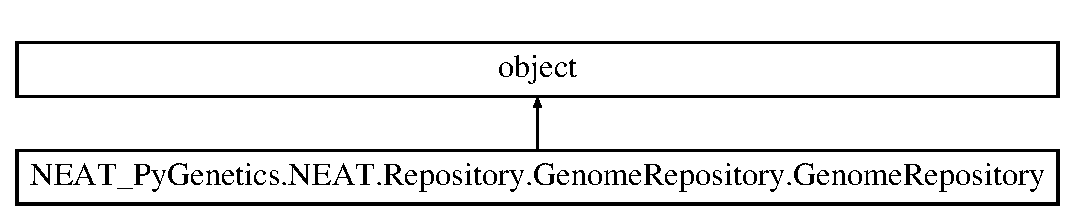
\includegraphics[height=2.000000cm]{class_n_e_a_t___py_genetics_1_1_n_e_a_t_1_1_repository_1_1_genome_repository_1_1_genome_repository}
\end{center}
\end{figure}
\subsection*{Public Member Functions}
\begin{DoxyCompactItemize}
\item 
def {\bfseries \+\_\+\+\_\+init\+\_\+\+\_\+}\hypertarget{class_n_e_a_t___py_genetics_1_1_n_e_a_t_1_1_repository_1_1_genome_repository_1_1_genome_repository_a2d5029444baeba1137a19954fbdc5192}{}\label{class_n_e_a_t___py_genetics_1_1_n_e_a_t_1_1_repository_1_1_genome_repository_1_1_genome_repository_a2d5029444baeba1137a19954fbdc5192}

\item 
def \hyperlink{class_n_e_a_t___py_genetics_1_1_n_e_a_t_1_1_repository_1_1_genome_repository_1_1_genome_repository_a02f46e4d4d2d09b0ac2b69174f49e129}{get\+\_\+current\+\_\+population} (self)
\item 
def {\bfseries get\+\_\+genome\+\_\+by\+\_\+id}\hypertarget{class_n_e_a_t___py_genetics_1_1_n_e_a_t_1_1_repository_1_1_genome_repository_1_1_genome_repository_ac55f0529efead778623d6e3eadafa138}{}\label{class_n_e_a_t___py_genetics_1_1_n_e_a_t_1_1_repository_1_1_genome_repository_1_1_genome_repository_ac55f0529efead778623d6e3eadafa138}

\item 
def {\bfseries get\+\_\+genomes\+\_\+in\+\_\+cluster}\hypertarget{class_n_e_a_t___py_genetics_1_1_n_e_a_t_1_1_repository_1_1_genome_repository_1_1_genome_repository_a307127db97bbcb6ef6bbb2000e64d36c}{}\label{class_n_e_a_t___py_genetics_1_1_n_e_a_t_1_1_repository_1_1_genome_repository_1_1_genome_repository_a307127db97bbcb6ef6bbb2000e64d36c}

\item 
def {\bfseries insert\+\_\+genome}\hypertarget{class_n_e_a_t___py_genetics_1_1_n_e_a_t_1_1_repository_1_1_genome_repository_1_1_genome_repository_ac5457262e579905f051b3a0e4f14cbae}{}\label{class_n_e_a_t___py_genetics_1_1_n_e_a_t_1_1_repository_1_1_genome_repository_1_1_genome_repository_ac5457262e579905f051b3a0e4f14cbae}

\item 
def {\bfseries insert\+\_\+genomes}\hypertarget{class_n_e_a_t___py_genetics_1_1_n_e_a_t_1_1_repository_1_1_genome_repository_1_1_genome_repository_ae5b9ba3a9e6586e42cefdd9daf1379b3}{}\label{class_n_e_a_t___py_genetics_1_1_n_e_a_t_1_1_repository_1_1_genome_repository_1_1_genome_repository_ae5b9ba3a9e6586e42cefdd9daf1379b3}

\item 
def {\bfseries update\+\_\+genome}\hypertarget{class_n_e_a_t___py_genetics_1_1_n_e_a_t_1_1_repository_1_1_genome_repository_1_1_genome_repository_a62c182ec66b0b0f2e444f6bd62f212a2}{}\label{class_n_e_a_t___py_genetics_1_1_n_e_a_t_1_1_repository_1_1_genome_repository_1_1_genome_repository_a62c182ec66b0b0f2e444f6bd62f212a2}

\item 
def {\bfseries update\+\_\+genomes}\hypertarget{class_n_e_a_t___py_genetics_1_1_n_e_a_t_1_1_repository_1_1_genome_repository_1_1_genome_repository_af596e230a4ae914fda99e8f8dfdab8a3}{}\label{class_n_e_a_t___py_genetics_1_1_n_e_a_t_1_1_repository_1_1_genome_repository_1_1_genome_repository_af596e230a4ae914fda99e8f8dfdab8a3}

\item 
def {\bfseries disable\+\_\+genome}\hypertarget{class_n_e_a_t___py_genetics_1_1_n_e_a_t_1_1_repository_1_1_genome_repository_1_1_genome_repository_a9a4f5e6dc63ce8a858a79bdb331cc62c}{}\label{class_n_e_a_t___py_genetics_1_1_n_e_a_t_1_1_repository_1_1_genome_repository_1_1_genome_repository_a9a4f5e6dc63ce8a858a79bdb331cc62c}

\item 
def {\bfseries disable\+\_\+genomes}\hypertarget{class_n_e_a_t___py_genetics_1_1_n_e_a_t_1_1_repository_1_1_genome_repository_1_1_genome_repository_aad8da608f4c1919e72453f1671761b8e}{}\label{class_n_e_a_t___py_genetics_1_1_n_e_a_t_1_1_repository_1_1_genome_repository_1_1_genome_repository_aad8da608f4c1919e72453f1671761b8e}

\item 
def {\bfseries update\+\_\+genome\+\_\+fitness}\hypertarget{class_n_e_a_t___py_genetics_1_1_n_e_a_t_1_1_repository_1_1_genome_repository_1_1_genome_repository_a89e1f1e4680f135c1eba0f8d13314896}{}\label{class_n_e_a_t___py_genetics_1_1_n_e_a_t_1_1_repository_1_1_genome_repository_1_1_genome_repository_a89e1f1e4680f135c1eba0f8d13314896}

\item 
def {\bfseries update\+\_\+genomes\+\_\+fitness}\hypertarget{class_n_e_a_t___py_genetics_1_1_n_e_a_t_1_1_repository_1_1_genome_repository_1_1_genome_repository_a6e90ef99f78be7ecddc26d8b73416116}{}\label{class_n_e_a_t___py_genetics_1_1_n_e_a_t_1_1_repository_1_1_genome_repository_1_1_genome_repository_a6e90ef99f78be7ecddc26d8b73416116}

\item 
def {\bfseries update\+\_\+genome\+\_\+cluster}\hypertarget{class_n_e_a_t___py_genetics_1_1_n_e_a_t_1_1_repository_1_1_genome_repository_1_1_genome_repository_a1709665aff216c7567cbc079bc5135c8}{}\label{class_n_e_a_t___py_genetics_1_1_n_e_a_t_1_1_repository_1_1_genome_repository_1_1_genome_repository_a1709665aff216c7567cbc079bc5135c8}

\end{DoxyCompactItemize}
\subsection*{Static Public Member Functions}
\begin{DoxyCompactItemize}
\item 
def \hyperlink{class_n_e_a_t___py_genetics_1_1_n_e_a_t_1_1_repository_1_1_genome_repository_1_1_genome_repository_a2ac10279f99269dc45fb9ed047c37fb9}{get\+\_\+new\+\_\+genome} ()
\end{DoxyCompactItemize}
\subsection*{Static Public Attributes}
\begin{DoxyCompactItemize}
\item 
{\bfseries genome}\hypertarget{class_n_e_a_t___py_genetics_1_1_n_e_a_t_1_1_repository_1_1_genome_repository_1_1_genome_repository_a23662b9337cfca1f402b206989747f45}{}\label{class_n_e_a_t___py_genetics_1_1_n_e_a_t_1_1_repository_1_1_genome_repository_1_1_genome_repository_a23662b9337cfca1f402b206989747f45}

\item 
{\bfseries cluster}\hypertarget{class_n_e_a_t___py_genetics_1_1_n_e_a_t_1_1_repository_1_1_genome_repository_1_1_genome_repository_a8932d6257b6a5e28ddc6aa822585eef0}{}\label{class_n_e_a_t___py_genetics_1_1_n_e_a_t_1_1_repository_1_1_genome_repository_1_1_genome_repository_a8932d6257b6a5e28ddc6aa822585eef0}

\end{DoxyCompactItemize}


\subsection{Detailed Description}


Definition at line 8 of file Genome\+Repository.\+py.



\subsection{Member Function Documentation}
\index{N\+E\+A\+T\+\_\+\+Py\+Genetics\+::\+N\+E\+A\+T\+::\+Repository\+::\+Genome\+Repository\+::\+Genome\+Repository@{N\+E\+A\+T\+\_\+\+Py\+Genetics\+::\+N\+E\+A\+T\+::\+Repository\+::\+Genome\+Repository\+::\+Genome\+Repository}!get\+\_\+current\+\_\+population@{get\+\_\+current\+\_\+population}}
\index{get\+\_\+current\+\_\+population@{get\+\_\+current\+\_\+population}!N\+E\+A\+T\+\_\+\+Py\+Genetics\+::\+N\+E\+A\+T\+::\+Repository\+::\+Genome\+Repository\+::\+Genome\+Repository@{N\+E\+A\+T\+\_\+\+Py\+Genetics\+::\+N\+E\+A\+T\+::\+Repository\+::\+Genome\+Repository\+::\+Genome\+Repository}}
\subsubsection[{\texorpdfstring{get\+\_\+current\+\_\+population(self)}{get_current_population(self)}}]{\setlength{\rightskip}{0pt plus 5cm}def N\+E\+A\+T\+\_\+\+Py\+Genetics.\+N\+E\+A\+T.\+Repository.\+Genome\+Repository.\+Genome\+Repository.\+get\+\_\+current\+\_\+population (
\begin{DoxyParamCaption}
\item[{}]{self, }
\item[{}]{Iterable, }
\item[{}]{Storage\+Genome}
\end{DoxyParamCaption}
)}\hypertarget{class_n_e_a_t___py_genetics_1_1_n_e_a_t_1_1_repository_1_1_genome_repository_1_1_genome_repository_a02f46e4d4d2d09b0ac2b69174f49e129}{}\label{class_n_e_a_t___py_genetics_1_1_n_e_a_t_1_1_repository_1_1_genome_repository_1_1_genome_repository_a02f46e4d4d2d09b0ac2b69174f49e129}
\begin{DoxyVerb}:return: Iterable[StorageGenomes] which are alive
\end{DoxyVerb}
 

Definition at line 26 of file Genome\+Repository.\+py.

\index{N\+E\+A\+T\+\_\+\+Py\+Genetics\+::\+N\+E\+A\+T\+::\+Repository\+::\+Genome\+Repository\+::\+Genome\+Repository@{N\+E\+A\+T\+\_\+\+Py\+Genetics\+::\+N\+E\+A\+T\+::\+Repository\+::\+Genome\+Repository\+::\+Genome\+Repository}!get\+\_\+new\+\_\+genome@{get\+\_\+new\+\_\+genome}}
\index{get\+\_\+new\+\_\+genome@{get\+\_\+new\+\_\+genome}!N\+E\+A\+T\+\_\+\+Py\+Genetics\+::\+N\+E\+A\+T\+::\+Repository\+::\+Genome\+Repository\+::\+Genome\+Repository@{N\+E\+A\+T\+\_\+\+Py\+Genetics\+::\+N\+E\+A\+T\+::\+Repository\+::\+Genome\+Repository\+::\+Genome\+Repository}}
\subsubsection[{\texorpdfstring{get\+\_\+new\+\_\+genome()}{get_new_genome()}}]{\setlength{\rightskip}{0pt plus 5cm}def N\+E\+A\+T\+\_\+\+Py\+Genetics.\+N\+E\+A\+T.\+Repository.\+Genome\+Repository.\+Genome\+Repository.\+get\+\_\+new\+\_\+genome (
\begin{DoxyParamCaption}
\item[{}]{Storage\+Genome}
\end{DoxyParamCaption}
)\hspace{0.3cm}{\ttfamily [static]}}\hypertarget{class_n_e_a_t___py_genetics_1_1_n_e_a_t_1_1_repository_1_1_genome_repository_1_1_genome_repository_a2ac10279f99269dc45fb9ed047c37fb9}{}\label{class_n_e_a_t___py_genetics_1_1_n_e_a_t_1_1_repository_1_1_genome_repository_1_1_genome_repository_a2ac10279f99269dc45fb9ed047c37fb9}
\begin{DoxyVerb}:return: StorageGenome new StorageGenome
\end{DoxyVerb}
 

Definition at line 18 of file Genome\+Repository.\+py.



The documentation for this class was generated from the following file\+:\begin{DoxyCompactItemize}
\item 
N\+E\+A\+T/\+Repository/Genome\+Repository.\+py\end{DoxyCompactItemize}

\hypertarget{class_n_e_a_t___py_genetics_1_1_n_e_a_t_1_1_analyst_1_1_genome_selector_1_1_genome_selector}{}\section{N\+E\+A\+T\+\_\+\+Py\+Genetics.\+N\+E\+A\+T.\+Analyst.\+Genome\+Selector.\+Genome\+Selector Class Reference}
\label{class_n_e_a_t___py_genetics_1_1_n_e_a_t_1_1_analyst_1_1_genome_selector_1_1_genome_selector}\index{N\+E\+A\+T\+\_\+\+Py\+Genetics.\+N\+E\+A\+T.\+Analyst.\+Genome\+Selector.\+Genome\+Selector@{N\+E\+A\+T\+\_\+\+Py\+Genetics.\+N\+E\+A\+T.\+Analyst.\+Genome\+Selector.\+Genome\+Selector}}
Inheritance diagram for N\+E\+A\+T\+\_\+\+Py\+Genetics.\+N\+E\+A\+T.\+Analyst.\+Genome\+Selector.\+Genome\+Selector\+:\begin{figure}[H]
\begin{center}
\leavevmode
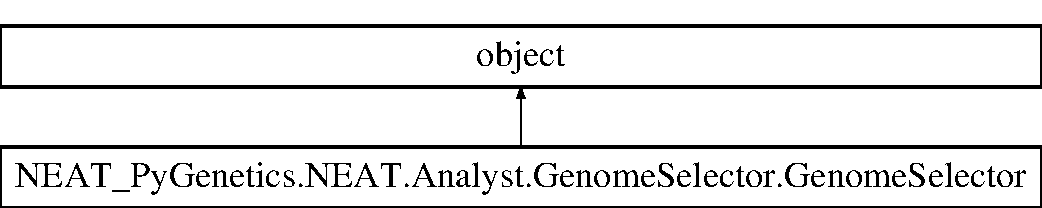
\includegraphics[height=2.000000cm]{class_n_e_a_t___py_genetics_1_1_n_e_a_t_1_1_analyst_1_1_genome_selector_1_1_genome_selector}
\end{center}
\end{figure}
\subsection*{Public Member Functions}
\begin{DoxyCompactItemize}
\item 
def {\bfseries \+\_\+\+\_\+init\+\_\+\+\_\+}\hypertarget{class_n_e_a_t___py_genetics_1_1_n_e_a_t_1_1_analyst_1_1_genome_selector_1_1_genome_selector_a92cb92afdabf4246963cf8214c9baa76}{}\label{class_n_e_a_t___py_genetics_1_1_n_e_a_t_1_1_analyst_1_1_genome_selector_1_1_genome_selector_a92cb92afdabf4246963cf8214c9baa76}

\item 
def {\bfseries get\+\_\+genomes\+\_\+in\+\_\+cluster}\hypertarget{class_n_e_a_t___py_genetics_1_1_n_e_a_t_1_1_analyst_1_1_genome_selector_1_1_genome_selector_aae7092166920c907176530a60deda37d}{}\label{class_n_e_a_t___py_genetics_1_1_n_e_a_t_1_1_analyst_1_1_genome_selector_1_1_genome_selector_aae7092166920c907176530a60deda37d}

\item 
def {\bfseries get\+\_\+cluster\+\_\+area\+\_\+sorted\+\_\+by\+\_\+fitness}\hypertarget{class_n_e_a_t___py_genetics_1_1_n_e_a_t_1_1_analyst_1_1_genome_selector_1_1_genome_selector_a2fb8600454d9d808158dbe3ace6b4952}{}\label{class_n_e_a_t___py_genetics_1_1_n_e_a_t_1_1_analyst_1_1_genome_selector_1_1_genome_selector_a2fb8600454d9d808158dbe3ace6b4952}

\item 
def {\bfseries select\+\_\+genomes\+\_\+for\+\_\+breeding}\hypertarget{class_n_e_a_t___py_genetics_1_1_n_e_a_t_1_1_analyst_1_1_genome_selector_1_1_genome_selector_a938d385b8d73983a5e9abf75a80f03f5}{}\label{class_n_e_a_t___py_genetics_1_1_n_e_a_t_1_1_analyst_1_1_genome_selector_1_1_genome_selector_a938d385b8d73983a5e9abf75a80f03f5}

\item 
def {\bfseries select\+\_\+genomes\+\_\+for\+\_\+mutation}\hypertarget{class_n_e_a_t___py_genetics_1_1_n_e_a_t_1_1_analyst_1_1_genome_selector_1_1_genome_selector_af335a5342b0a1695c52d61274c83b0bf}{}\label{class_n_e_a_t___py_genetics_1_1_n_e_a_t_1_1_analyst_1_1_genome_selector_1_1_genome_selector_af335a5342b0a1695c52d61274c83b0bf}

\item 
def \hyperlink{class_n_e_a_t___py_genetics_1_1_n_e_a_t_1_1_analyst_1_1_genome_selector_1_1_genome_selector_a9e1d64bae210147a47049f1c8c389bfc}{select\+\_\+clusters\+\_\+for\+\_\+combination} (self)
\item 
def {\bfseries select\+\_\+cluster\+\_\+combinations}\hypertarget{class_n_e_a_t___py_genetics_1_1_n_e_a_t_1_1_analyst_1_1_genome_selector_1_1_genome_selector_a08b5d1264a5dadc1ec98affabf1ab76d}{}\label{class_n_e_a_t___py_genetics_1_1_n_e_a_t_1_1_analyst_1_1_genome_selector_1_1_genome_selector_a08b5d1264a5dadc1ec98affabf1ab76d}

\item 
def \hyperlink{class_n_e_a_t___py_genetics_1_1_n_e_a_t_1_1_analyst_1_1_genome_selector_1_1_genome_selector_a1016a10b5301bd2a1fd770dceda6644b}{select\+\_\+clusters\+\_\+for\+\_\+discarding} (self)
\item 
def \hyperlink{class_n_e_a_t___py_genetics_1_1_n_e_a_t_1_1_analyst_1_1_genome_selector_1_1_genome_selector_af7cd898b9a5bbc1e2e407256a385f865}{select\+\_\+genomes\+\_\+for\+\_\+discarding} (self)
\end{DoxyCompactItemize}
\subsection*{Static Public Attributes}
\begin{DoxyCompactItemize}
\item 
{\bfseries genome\+\_\+repository}\hypertarget{class_n_e_a_t___py_genetics_1_1_n_e_a_t_1_1_analyst_1_1_genome_selector_1_1_genome_selector_aabb39abd6a1fcfa61f9b8eb4662e00db}{}\label{class_n_e_a_t___py_genetics_1_1_n_e_a_t_1_1_analyst_1_1_genome_selector_1_1_genome_selector_aabb39abd6a1fcfa61f9b8eb4662e00db}

\item 
{\bfseries cluster\+\_\+repository}\hypertarget{class_n_e_a_t___py_genetics_1_1_n_e_a_t_1_1_analyst_1_1_genome_selector_1_1_genome_selector_ad3561e93fc8fdd2c51ffec388ddc4c7e}{}\label{class_n_e_a_t___py_genetics_1_1_n_e_a_t_1_1_analyst_1_1_genome_selector_1_1_genome_selector_ad3561e93fc8fdd2c51ffec388ddc4c7e}

\item 
{\bfseries selection\+\_\+parameters}\hypertarget{class_n_e_a_t___py_genetics_1_1_n_e_a_t_1_1_analyst_1_1_genome_selector_1_1_genome_selector_af6ab170d7eef08b15d79eabb074ade5e}{}\label{class_n_e_a_t___py_genetics_1_1_n_e_a_t_1_1_analyst_1_1_genome_selector_1_1_genome_selector_af6ab170d7eef08b15d79eabb074ade5e}

\item 
{\bfseries genomes}\hypertarget{class_n_e_a_t___py_genetics_1_1_n_e_a_t_1_1_analyst_1_1_genome_selector_1_1_genome_selector_affce7cea247dd2a869d83fbcc67f9f78}{}\label{class_n_e_a_t___py_genetics_1_1_n_e_a_t_1_1_analyst_1_1_genome_selector_1_1_genome_selector_affce7cea247dd2a869d83fbcc67f9f78}

\item 
{\bfseries clusters}\hypertarget{class_n_e_a_t___py_genetics_1_1_n_e_a_t_1_1_analyst_1_1_genome_selector_1_1_genome_selector_a65680f48e6b7e8f218f8536420a665db}{}\label{class_n_e_a_t___py_genetics_1_1_n_e_a_t_1_1_analyst_1_1_genome_selector_1_1_genome_selector_a65680f48e6b7e8f218f8536420a665db}

\item 
{\bfseries key}\hypertarget{class_n_e_a_t___py_genetics_1_1_n_e_a_t_1_1_analyst_1_1_genome_selector_1_1_genome_selector_a59881db1a9d315dd4019aad7d52eeeb2}{}\label{class_n_e_a_t___py_genetics_1_1_n_e_a_t_1_1_analyst_1_1_genome_selector_1_1_genome_selector_a59881db1a9d315dd4019aad7d52eeeb2}

\item 
{\bfseries start}\hypertarget{class_n_e_a_t___py_genetics_1_1_n_e_a_t_1_1_analyst_1_1_genome_selector_1_1_genome_selector_a41d6d1538df7134f2f31519ff49f6c58}{}\label{class_n_e_a_t___py_genetics_1_1_n_e_a_t_1_1_analyst_1_1_genome_selector_1_1_genome_selector_a41d6d1538df7134f2f31519ff49f6c58}

\item 
{\bfseries end}\hypertarget{class_n_e_a_t___py_genetics_1_1_n_e_a_t_1_1_analyst_1_1_genome_selector_1_1_genome_selector_a9531d1391e7501950602af5dd854a43a}{}\label{class_n_e_a_t___py_genetics_1_1_n_e_a_t_1_1_analyst_1_1_genome_selector_1_1_genome_selector_a9531d1391e7501950602af5dd854a43a}

\item 
{\bfseries result}\hypertarget{class_n_e_a_t___py_genetics_1_1_n_e_a_t_1_1_analyst_1_1_genome_selector_1_1_genome_selector_af361031b936449d59bedda05b9363d13}{}\label{class_n_e_a_t___py_genetics_1_1_n_e_a_t_1_1_analyst_1_1_genome_selector_1_1_genome_selector_af361031b936449d59bedda05b9363d13}

\item 
{\bfseries genome\+\_\+one}\hypertarget{class_n_e_a_t___py_genetics_1_1_n_e_a_t_1_1_analyst_1_1_genome_selector_1_1_genome_selector_afa3ff139e2ad867f5746aee243fd9aa1}{}\label{class_n_e_a_t___py_genetics_1_1_n_e_a_t_1_1_analyst_1_1_genome_selector_1_1_genome_selector_afa3ff139e2ad867f5746aee243fd9aa1}

\item 
{\bfseries genome\+\_\+two}\hypertarget{class_n_e_a_t___py_genetics_1_1_n_e_a_t_1_1_analyst_1_1_genome_selector_1_1_genome_selector_a8ea3993f52a51fe0d93b331eb2b78a8d}{}\label{class_n_e_a_t___py_genetics_1_1_n_e_a_t_1_1_analyst_1_1_genome_selector_1_1_genome_selector_a8ea3993f52a51fe0d93b331eb2b78a8d}

\item 
{\bfseries seats\+\_\+to\+\_\+mutation}\hypertarget{class_n_e_a_t___py_genetics_1_1_n_e_a_t_1_1_analyst_1_1_genome_selector_1_1_genome_selector_a22cb93426797917839ba925a79e51a36}{}\label{class_n_e_a_t___py_genetics_1_1_n_e_a_t_1_1_analyst_1_1_genome_selector_1_1_genome_selector_a22cb93426797917839ba925a79e51a36}

\item 
{\bfseries step}\hypertarget{class_n_e_a_t___py_genetics_1_1_n_e_a_t_1_1_analyst_1_1_genome_selector_1_1_genome_selector_af8c8af7836b5ae5b52f6688c1266bb06}{}\label{class_n_e_a_t___py_genetics_1_1_n_e_a_t_1_1_analyst_1_1_genome_selector_1_1_genome_selector_af8c8af7836b5ae5b52f6688c1266bb06}

\item 
{\bfseries genomes1}\hypertarget{class_n_e_a_t___py_genetics_1_1_n_e_a_t_1_1_analyst_1_1_genome_selector_1_1_genome_selector_a2b86adfa98c72c3ce406e95fce29a9ad}{}\label{class_n_e_a_t___py_genetics_1_1_n_e_a_t_1_1_analyst_1_1_genome_selector_1_1_genome_selector_a2b86adfa98c72c3ce406e95fce29a9ad}

\item 
{\bfseries genomes2}\hypertarget{class_n_e_a_t___py_genetics_1_1_n_e_a_t_1_1_analyst_1_1_genome_selector_1_1_genome_selector_aff1676f8a3e91f03ef133d445fd111b8}{}\label{class_n_e_a_t___py_genetics_1_1_n_e_a_t_1_1_analyst_1_1_genome_selector_1_1_genome_selector_aff1676f8a3e91f03ef133d445fd111b8}

\item 
{\bfseries g1}\hypertarget{class_n_e_a_t___py_genetics_1_1_n_e_a_t_1_1_analyst_1_1_genome_selector_1_1_genome_selector_a66bc085d9c0e2b4ce121fd3c4d4ec226}{}\label{class_n_e_a_t___py_genetics_1_1_n_e_a_t_1_1_analyst_1_1_genome_selector_1_1_genome_selector_a66bc085d9c0e2b4ce121fd3c4d4ec226}

\item 
{\bfseries g2}\hypertarget{class_n_e_a_t___py_genetics_1_1_n_e_a_t_1_1_analyst_1_1_genome_selector_1_1_genome_selector_a335eeb80af660ac6ef6d5a8ca81fb95c}{}\label{class_n_e_a_t___py_genetics_1_1_n_e_a_t_1_1_analyst_1_1_genome_selector_1_1_genome_selector_a335eeb80af660ac6ef6d5a8ca81fb95c}

\end{DoxyCompactItemize}


\subsection{Detailed Description}


Definition at line 13 of file Genome\+Selector.\+py.



\subsection{Member Function Documentation}
\index{N\+E\+A\+T\+\_\+\+Py\+Genetics\+::\+N\+E\+A\+T\+::\+Analyst\+::\+Genome\+Selector\+::\+Genome\+Selector@{N\+E\+A\+T\+\_\+\+Py\+Genetics\+::\+N\+E\+A\+T\+::\+Analyst\+::\+Genome\+Selector\+::\+Genome\+Selector}!select\+\_\+clusters\+\_\+for\+\_\+combination@{select\+\_\+clusters\+\_\+for\+\_\+combination}}
\index{select\+\_\+clusters\+\_\+for\+\_\+combination@{select\+\_\+clusters\+\_\+for\+\_\+combination}!N\+E\+A\+T\+\_\+\+Py\+Genetics\+::\+N\+E\+A\+T\+::\+Analyst\+::\+Genome\+Selector\+::\+Genome\+Selector@{N\+E\+A\+T\+\_\+\+Py\+Genetics\+::\+N\+E\+A\+T\+::\+Analyst\+::\+Genome\+Selector\+::\+Genome\+Selector}}
\subsubsection[{\texorpdfstring{select\+\_\+clusters\+\_\+for\+\_\+combination(self)}{select_clusters_for_combination(self)}}]{\setlength{\rightskip}{0pt plus 5cm}def N\+E\+A\+T\+\_\+\+Py\+Genetics.\+N\+E\+A\+T.\+Analyst.\+Genome\+Selector.\+Genome\+Selector.\+select\+\_\+clusters\+\_\+for\+\_\+combination (
\begin{DoxyParamCaption}
\item[{}]{self, }
\item[{}]{Tuple, }
\item[{}]{Cluster, }
\item[{}]{Cluster}
\end{DoxyParamCaption}
)}\hypertarget{class_n_e_a_t___py_genetics_1_1_n_e_a_t_1_1_analyst_1_1_genome_selector_1_1_genome_selector_a9e1d64bae210147a47049f1c8c389bfc}{}\label{class_n_e_a_t___py_genetics_1_1_n_e_a_t_1_1_analyst_1_1_genome_selector_1_1_genome_selector_a9e1d64bae210147a47049f1c8c389bfc}
\begin{DoxyVerb}:return: Tuple[Cluster] cluster chosen for combination
\end{DoxyVerb}
 

Definition at line 106 of file Genome\+Selector.\+py.

\index{N\+E\+A\+T\+\_\+\+Py\+Genetics\+::\+N\+E\+A\+T\+::\+Analyst\+::\+Genome\+Selector\+::\+Genome\+Selector@{N\+E\+A\+T\+\_\+\+Py\+Genetics\+::\+N\+E\+A\+T\+::\+Analyst\+::\+Genome\+Selector\+::\+Genome\+Selector}!select\+\_\+clusters\+\_\+for\+\_\+discarding@{select\+\_\+clusters\+\_\+for\+\_\+discarding}}
\index{select\+\_\+clusters\+\_\+for\+\_\+discarding@{select\+\_\+clusters\+\_\+for\+\_\+discarding}!N\+E\+A\+T\+\_\+\+Py\+Genetics\+::\+N\+E\+A\+T\+::\+Analyst\+::\+Genome\+Selector\+::\+Genome\+Selector@{N\+E\+A\+T\+\_\+\+Py\+Genetics\+::\+N\+E\+A\+T\+::\+Analyst\+::\+Genome\+Selector\+::\+Genome\+Selector}}
\subsubsection[{\texorpdfstring{select\+\_\+clusters\+\_\+for\+\_\+discarding(self)}{select_clusters_for_discarding(self)}}]{\setlength{\rightskip}{0pt plus 5cm}def N\+E\+A\+T\+\_\+\+Py\+Genetics.\+N\+E\+A\+T.\+Analyst.\+Genome\+Selector.\+Genome\+Selector.\+select\+\_\+clusters\+\_\+for\+\_\+discarding (
\begin{DoxyParamCaption}
\item[{}]{self, }
\item[{}]{List, }
\item[{}]{Cluster}
\end{DoxyParamCaption}
)}\hypertarget{class_n_e_a_t___py_genetics_1_1_n_e_a_t_1_1_analyst_1_1_genome_selector_1_1_genome_selector_a1016a10b5301bd2a1fd770dceda6644b}{}\label{class_n_e_a_t___py_genetics_1_1_n_e_a_t_1_1_analyst_1_1_genome_selector_1_1_genome_selector_a1016a10b5301bd2a1fd770dceda6644b}
\begin{DoxyVerb}select x percentage (given by selection.conf "discarding_by_cluster_fitness") of Cluster sorted ascending
by fitness
:return: List of Cluster wanted to be discarded
\end{DoxyVerb}
 

Definition at line 137 of file Genome\+Selector.\+py.

\index{N\+E\+A\+T\+\_\+\+Py\+Genetics\+::\+N\+E\+A\+T\+::\+Analyst\+::\+Genome\+Selector\+::\+Genome\+Selector@{N\+E\+A\+T\+\_\+\+Py\+Genetics\+::\+N\+E\+A\+T\+::\+Analyst\+::\+Genome\+Selector\+::\+Genome\+Selector}!select\+\_\+genomes\+\_\+for\+\_\+discarding@{select\+\_\+genomes\+\_\+for\+\_\+discarding}}
\index{select\+\_\+genomes\+\_\+for\+\_\+discarding@{select\+\_\+genomes\+\_\+for\+\_\+discarding}!N\+E\+A\+T\+\_\+\+Py\+Genetics\+::\+N\+E\+A\+T\+::\+Analyst\+::\+Genome\+Selector\+::\+Genome\+Selector@{N\+E\+A\+T\+\_\+\+Py\+Genetics\+::\+N\+E\+A\+T\+::\+Analyst\+::\+Genome\+Selector\+::\+Genome\+Selector}}
\subsubsection[{\texorpdfstring{select\+\_\+genomes\+\_\+for\+\_\+discarding(self)}{select_genomes_for_discarding(self)}}]{\setlength{\rightskip}{0pt plus 5cm}def N\+E\+A\+T\+\_\+\+Py\+Genetics.\+N\+E\+A\+T.\+Analyst.\+Genome\+Selector.\+Genome\+Selector.\+select\+\_\+genomes\+\_\+for\+\_\+discarding (
\begin{DoxyParamCaption}
\item[{}]{self, }
\item[{}]{List, }
\item[{}]{Storage\+Genome}
\end{DoxyParamCaption}
)}\hypertarget{class_n_e_a_t___py_genetics_1_1_n_e_a_t_1_1_analyst_1_1_genome_selector_1_1_genome_selector_af7cd898b9a5bbc1e2e407256a385f865}{}\label{class_n_e_a_t___py_genetics_1_1_n_e_a_t_1_1_analyst_1_1_genome_selector_1_1_genome_selector_af7cd898b9a5bbc1e2e407256a385f865}
\begin{DoxyVerb}select "discarding_by_genome_fitness" percentage (in every Cluster) of genomes sorted ascending by fitness
:return: List of Genomes wanted to be discarded
\end{DoxyVerb}
 

Definition at line 150 of file Genome\+Selector.\+py.



The documentation for this class was generated from the following file\+:\begin{DoxyCompactItemize}
\item 
N\+E\+A\+T/\+Analyst/Genome\+Selector.\+py\end{DoxyCompactItemize}

\hypertarget{class_n_e_a_t___py_genetics_1_1_n_e_a_t_1_1_networking_1_1_commands_1_1_get_block_command_1_1_get_block_command}{}\section{N\+E\+A\+T\+\_\+\+Py\+Genetics.\+N\+E\+A\+T.\+Networking.\+Commands.\+Get\+Block\+Command.\+Get\+Block\+Command Class Reference}
\label{class_n_e_a_t___py_genetics_1_1_n_e_a_t_1_1_networking_1_1_commands_1_1_get_block_command_1_1_get_block_command}\index{N\+E\+A\+T\+\_\+\+Py\+Genetics.\+N\+E\+A\+T.\+Networking.\+Commands.\+Get\+Block\+Command.\+Get\+Block\+Command@{N\+E\+A\+T\+\_\+\+Py\+Genetics.\+N\+E\+A\+T.\+Networking.\+Commands.\+Get\+Block\+Command.\+Get\+Block\+Command}}
Inheritance diagram for N\+E\+A\+T\+\_\+\+Py\+Genetics.\+N\+E\+A\+T.\+Networking.\+Commands.\+Get\+Block\+Command.\+Get\+Block\+Command\+:\begin{figure}[H]
\begin{center}
\leavevmode
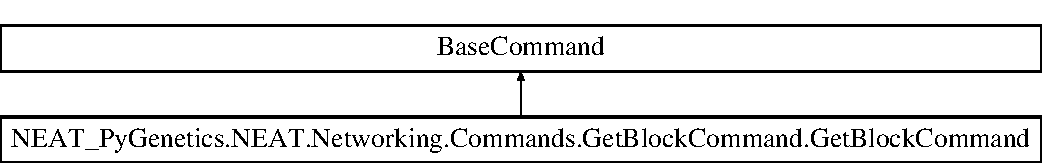
\includegraphics[height=2.000000cm]{class_n_e_a_t___py_genetics_1_1_n_e_a_t_1_1_networking_1_1_commands_1_1_get_block_command_1_1_get_block_command}
\end{center}
\end{figure}
\subsection*{Public Member Functions}
\begin{DoxyCompactItemize}
\item 
def {\bfseries \+\_\+\+\_\+init\+\_\+\+\_\+} (self)\hypertarget{class_n_e_a_t___py_genetics_1_1_n_e_a_t_1_1_networking_1_1_commands_1_1_get_block_command_1_1_get_block_command_ad58e15de61d1576383f64ad5e99ab691}{}\label{class_n_e_a_t___py_genetics_1_1_n_e_a_t_1_1_networking_1_1_commands_1_1_get_block_command_1_1_get_block_command_ad58e15de61d1576383f64ad5e99ab691}

\item 
def {\bfseries set\+\_\+block\+\_\+id}\hypertarget{class_n_e_a_t___py_genetics_1_1_n_e_a_t_1_1_networking_1_1_commands_1_1_get_block_command_1_1_get_block_command_abd6d6e34fe53e47b6bd8fe3be8a38f6c}{}\label{class_n_e_a_t___py_genetics_1_1_n_e_a_t_1_1_networking_1_1_commands_1_1_get_block_command_1_1_get_block_command_abd6d6e34fe53e47b6bd8fe3be8a38f6c}

\item 
def {\bfseries get\+\_\+block\+\_\+id} (self)\hypertarget{class_n_e_a_t___py_genetics_1_1_n_e_a_t_1_1_networking_1_1_commands_1_1_get_block_command_1_1_get_block_command_af58224cb2bfb479548d3ec42cdee8931}{}\label{class_n_e_a_t___py_genetics_1_1_n_e_a_t_1_1_networking_1_1_commands_1_1_get_block_command_1_1_get_block_command_af58224cb2bfb479548d3ec42cdee8931}

\item 
def {\bfseries get\+\_\+block} (self)\hypertarget{class_n_e_a_t___py_genetics_1_1_n_e_a_t_1_1_networking_1_1_commands_1_1_get_block_command_1_1_get_block_command_a0a4947f054e52700ca72c6f9f6ece118}{}\label{class_n_e_a_t___py_genetics_1_1_n_e_a_t_1_1_networking_1_1_commands_1_1_get_block_command_1_1_get_block_command_a0a4947f054e52700ca72c6f9f6ece118}

\item 
def {\bfseries get\+\_\+block\+\_\+size} (self)\hypertarget{class_n_e_a_t___py_genetics_1_1_n_e_a_t_1_1_networking_1_1_commands_1_1_get_block_command_1_1_get_block_command_a54eae8fc81e0a71fec523ce013637fc0}{}\label{class_n_e_a_t___py_genetics_1_1_n_e_a_t_1_1_networking_1_1_commands_1_1_get_block_command_1_1_get_block_command_a54eae8fc81e0a71fec523ce013637fc0}

\item 
def {\bfseries get\+\_\+resulting\+\_\+block\+\_\+id} (self)\hypertarget{class_n_e_a_t___py_genetics_1_1_n_e_a_t_1_1_networking_1_1_commands_1_1_get_block_command_1_1_get_block_command_aabe6091c8da0ef7cc5655cbcd1b7ec5b}{}\label{class_n_e_a_t___py_genetics_1_1_n_e_a_t_1_1_networking_1_1_commands_1_1_get_block_command_1_1_get_block_command_aabe6091c8da0ef7cc5655cbcd1b7ec5b}

\item 
def {\bfseries get\+\_\+next\+\_\+block\+\_\+id} (self)\hypertarget{class_n_e_a_t___py_genetics_1_1_n_e_a_t_1_1_networking_1_1_commands_1_1_get_block_command_1_1_get_block_command_a97eb16c91c2ebb7081518119585f55fe}{}\label{class_n_e_a_t___py_genetics_1_1_n_e_a_t_1_1_networking_1_1_commands_1_1_get_block_command_1_1_get_block_command_a97eb16c91c2ebb7081518119585f55fe}

\end{DoxyCompactItemize}


\subsection{Detailed Description}


Definition at line 6 of file Get\+Block\+Command.\+py.



The documentation for this class was generated from the following file\+:\begin{DoxyCompactItemize}
\item 
N\+E\+A\+T/\+Networking/\+Commands/Get\+Block\+Command.\+py\end{DoxyCompactItemize}

\hypertarget{class_n_e_a_t___py_genetics_1_1_n_e_a_t_1_1_networking_1_1_commands_1_1_get_outputs_command_1_1_get_outputs_command}{}\section{N\+E\+A\+T\+\_\+\+Py\+Genetics.\+N\+E\+A\+T.\+Networking.\+Commands.\+Get\+Outputs\+Command.\+Get\+Outputs\+Command Class Reference}
\label{class_n_e_a_t___py_genetics_1_1_n_e_a_t_1_1_networking_1_1_commands_1_1_get_outputs_command_1_1_get_outputs_command}\index{N\+E\+A\+T\+\_\+\+Py\+Genetics.\+N\+E\+A\+T.\+Networking.\+Commands.\+Get\+Outputs\+Command.\+Get\+Outputs\+Command@{N\+E\+A\+T\+\_\+\+Py\+Genetics.\+N\+E\+A\+T.\+Networking.\+Commands.\+Get\+Outputs\+Command.\+Get\+Outputs\+Command}}
Inheritance diagram for N\+E\+A\+T\+\_\+\+Py\+Genetics.\+N\+E\+A\+T.\+Networking.\+Commands.\+Get\+Outputs\+Command.\+Get\+Outputs\+Command\+:\begin{figure}[H]
\begin{center}
\leavevmode
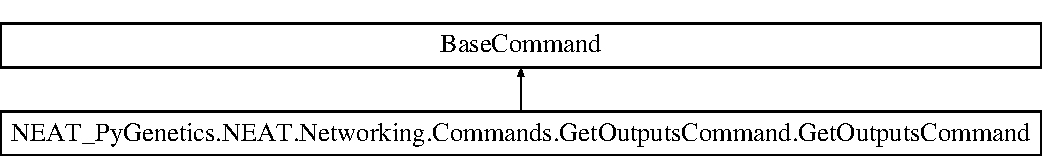
\includegraphics[height=2.000000cm]{class_n_e_a_t___py_genetics_1_1_n_e_a_t_1_1_networking_1_1_commands_1_1_get_outputs_command_1_1_get_outputs_command}
\end{center}
\end{figure}
\subsection*{Public Member Functions}
\begin{DoxyCompactItemize}
\item 
def {\bfseries \+\_\+\+\_\+init\+\_\+\+\_\+} (self)\hypertarget{class_n_e_a_t___py_genetics_1_1_n_e_a_t_1_1_networking_1_1_commands_1_1_get_outputs_command_1_1_get_outputs_command_a9cb7b34e60b60ab5b71843ba223ff626}{}\label{class_n_e_a_t___py_genetics_1_1_n_e_a_t_1_1_networking_1_1_commands_1_1_get_outputs_command_1_1_get_outputs_command_a9cb7b34e60b60ab5b71843ba223ff626}

\item 
def {\bfseries set\+\_\+block\+\_\+id}\hypertarget{class_n_e_a_t___py_genetics_1_1_n_e_a_t_1_1_networking_1_1_commands_1_1_get_outputs_command_1_1_get_outputs_command_a8ec7f2dc4780ec36b72c7fbff9492621}{}\label{class_n_e_a_t___py_genetics_1_1_n_e_a_t_1_1_networking_1_1_commands_1_1_get_outputs_command_1_1_get_outputs_command_a8ec7f2dc4780ec36b72c7fbff9492621}

\item 
def {\bfseries get\+\_\+block\+\_\+id} (self)\hypertarget{class_n_e_a_t___py_genetics_1_1_n_e_a_t_1_1_networking_1_1_commands_1_1_get_outputs_command_1_1_get_outputs_command_af1c805c74a7c01ff8314f84f8461f25c}{}\label{class_n_e_a_t___py_genetics_1_1_n_e_a_t_1_1_networking_1_1_commands_1_1_get_outputs_command_1_1_get_outputs_command_af1c805c74a7c01ff8314f84f8461f25c}

\end{DoxyCompactItemize}


\subsection{Detailed Description}


Definition at line 3 of file Get\+Outputs\+Command.\+py.



The documentation for this class was generated from the following file\+:\begin{DoxyCompactItemize}
\item 
N\+E\+A\+T/\+Networking/\+Commands/Get\+Outputs\+Command.\+py\end{DoxyCompactItemize}

\hypertarget{class_n_e_a_t___py_genetics_1_1_n_e_a_t_1_1_error_handling_1_1_exceptions_1_1_input_missing_exce0434cd2f533c4f8b0f57070fd8d9df81}{}\section{N\+E\+A\+T\+\_\+\+Py\+Genetics.\+N\+E\+A\+T.\+Error\+Handling.\+Exceptions.\+Input\+Missing\+Exception.\+Input\+Missing\+Exception Class Reference}
\label{class_n_e_a_t___py_genetics_1_1_n_e_a_t_1_1_error_handling_1_1_exceptions_1_1_input_missing_exce0434cd2f533c4f8b0f57070fd8d9df81}\index{N\+E\+A\+T\+\_\+\+Py\+Genetics.\+N\+E\+A\+T.\+Error\+Handling.\+Exceptions.\+Input\+Missing\+Exception.\+Input\+Missing\+Exception@{N\+E\+A\+T\+\_\+\+Py\+Genetics.\+N\+E\+A\+T.\+Error\+Handling.\+Exceptions.\+Input\+Missing\+Exception.\+Input\+Missing\+Exception}}
Inheritance diagram for N\+E\+A\+T\+\_\+\+Py\+Genetics.\+N\+E\+A\+T.\+Error\+Handling.\+Exceptions.\+Input\+Missing\+Exception.\+Input\+Missing\+Exception\+:\begin{figure}[H]
\begin{center}
\leavevmode
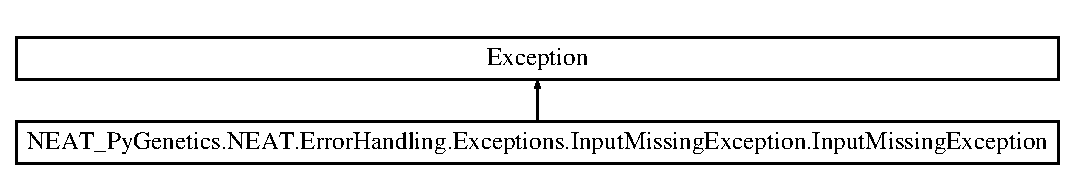
\includegraphics[height=1.971831cm]{class_n_e_a_t___py_genetics_1_1_n_e_a_t_1_1_error_handling_1_1_exceptions_1_1_input_missing_exce0434cd2f533c4f8b0f57070fd8d9df81}
\end{center}
\end{figure}
\subsection*{Public Member Functions}
\begin{DoxyCompactItemize}
\item 
def {\bfseries \+\_\+\+\_\+init\+\_\+\+\_\+} (self, message, errors=None)\hypertarget{class_n_e_a_t___py_genetics_1_1_n_e_a_t_1_1_error_handling_1_1_exceptions_1_1_input_missing_exce0434cd2f533c4f8b0f57070fd8d9df81_ad099b1a8bf35220cc7d2a47d4469d749}{}\label{class_n_e_a_t___py_genetics_1_1_n_e_a_t_1_1_error_handling_1_1_exceptions_1_1_input_missing_exce0434cd2f533c4f8b0f57070fd8d9df81_ad099b1a8bf35220cc7d2a47d4469d749}

\end{DoxyCompactItemize}


\subsection{Detailed Description}


Definition at line 1 of file Input\+Missing\+Exception.\+py.



The documentation for this class was generated from the following file\+:\begin{DoxyCompactItemize}
\item 
N\+E\+A\+T/\+Error\+Handling/\+Exceptions/Input\+Missing\+Exception.\+py\end{DoxyCompactItemize}

\hypertarget{class_n_e_a_t___py_genetics_1_1_n_e_a_t_1_1_networking_1_1_server_1_1_j_s_o_n_socket_1_1_j_s_o_n_socket}{}\section{N\+E\+A\+T\+\_\+\+Py\+Genetics.\+N\+E\+A\+T.\+Networking.\+Server.\+J\+S\+O\+N\+Socket.\+J\+S\+O\+N\+Socket Class Reference}
\label{class_n_e_a_t___py_genetics_1_1_n_e_a_t_1_1_networking_1_1_server_1_1_j_s_o_n_socket_1_1_j_s_o_n_socket}\index{N\+E\+A\+T\+\_\+\+Py\+Genetics.\+N\+E\+A\+T.\+Networking.\+Server.\+J\+S\+O\+N\+Socket.\+J\+S\+O\+N\+Socket@{N\+E\+A\+T\+\_\+\+Py\+Genetics.\+N\+E\+A\+T.\+Networking.\+Server.\+J\+S\+O\+N\+Socket.\+J\+S\+O\+N\+Socket}}
Inheritance diagram for N\+E\+A\+T\+\_\+\+Py\+Genetics.\+N\+E\+A\+T.\+Networking.\+Server.\+J\+S\+O\+N\+Socket.\+J\+S\+O\+N\+Socket\+:\begin{figure}[H]
\begin{center}
\leavevmode
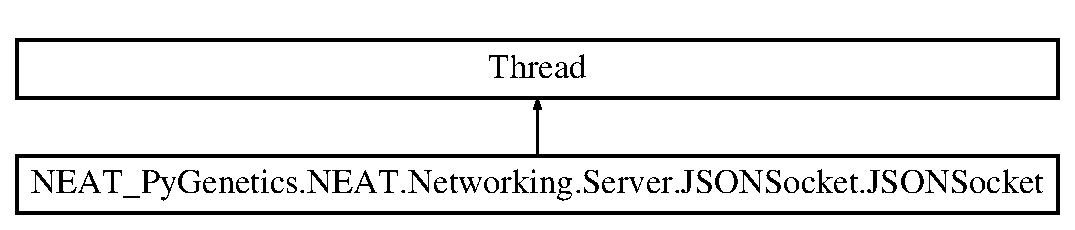
\includegraphics[height=2.000000cm]{class_n_e_a_t___py_genetics_1_1_n_e_a_t_1_1_networking_1_1_server_1_1_j_s_o_n_socket_1_1_j_s_o_n_socket}
\end{center}
\end{figure}
\subsection*{Public Member Functions}
\begin{DoxyCompactItemize}
\item 
def {\bfseries \+\_\+\+\_\+init\+\_\+\+\_\+} (self, server\+\_\+address, server\+\_\+port, header\+\_\+size=16, chunk\+\_\+size=1024)\hypertarget{class_n_e_a_t___py_genetics_1_1_n_e_a_t_1_1_networking_1_1_server_1_1_j_s_o_n_socket_1_1_j_s_o_n_socket_a95dd555e4124ce36a47d00e3b62b597a}{}\label{class_n_e_a_t___py_genetics_1_1_n_e_a_t_1_1_networking_1_1_server_1_1_j_s_o_n_socket_1_1_j_s_o_n_socket_a95dd555e4124ce36a47d00e3b62b597a}

\item 
def {\bfseries socket\+\_\+alive} (self)\hypertarget{class_n_e_a_t___py_genetics_1_1_n_e_a_t_1_1_networking_1_1_server_1_1_j_s_o_n_socket_1_1_j_s_o_n_socket_a05c99b2b4e7b4552155560f5fad0b939}{}\label{class_n_e_a_t___py_genetics_1_1_n_e_a_t_1_1_networking_1_1_server_1_1_j_s_o_n_socket_1_1_j_s_o_n_socket_a05c99b2b4e7b4552155560f5fad0b939}

\item 
def {\bfseries close\+\_\+connection} (self)\hypertarget{class_n_e_a_t___py_genetics_1_1_n_e_a_t_1_1_networking_1_1_server_1_1_j_s_o_n_socket_1_1_j_s_o_n_socket_a196c88e61cbc698f1012a5561f85f6d0}{}\label{class_n_e_a_t___py_genetics_1_1_n_e_a_t_1_1_networking_1_1_server_1_1_j_s_o_n_socket_1_1_j_s_o_n_socket_a196c88e61cbc698f1012a5561f85f6d0}

\item 
def {\bfseries send\+\_\+dict}\hypertarget{class_n_e_a_t___py_genetics_1_1_n_e_a_t_1_1_networking_1_1_server_1_1_j_s_o_n_socket_1_1_j_s_o_n_socket_a104209f938a7b47d91692face1dc0569}{}\label{class_n_e_a_t___py_genetics_1_1_n_e_a_t_1_1_networking_1_1_server_1_1_j_s_o_n_socket_1_1_j_s_o_n_socket_a104209f938a7b47d91692face1dc0569}

\item 
def {\bfseries receive\+\_\+dict} (self)\hypertarget{class_n_e_a_t___py_genetics_1_1_n_e_a_t_1_1_networking_1_1_server_1_1_j_s_o_n_socket_1_1_j_s_o_n_socket_a2bc8b4e45a2e94d386c98caba0ecce14}{}\label{class_n_e_a_t___py_genetics_1_1_n_e_a_t_1_1_networking_1_1_server_1_1_j_s_o_n_socket_1_1_j_s_o_n_socket_a2bc8b4e45a2e94d386c98caba0ecce14}

\end{DoxyCompactItemize}


\subsection{Detailed Description}


Definition at line 9 of file J\+S\+O\+N\+Socket.\+py.



The documentation for this class was generated from the following file\+:\begin{DoxyCompactItemize}
\item 
N\+E\+A\+T/\+Networking/\+Server/J\+S\+O\+N\+Socket.\+py\end{DoxyCompactItemize}

\hypertarget{class_n_e_a_t___py_genetics_1_1_n_e_a_t_1_1_logging_1_1_logger_1_1_logger}{}\section{N\+E\+A\+T\+\_\+\+Py\+Genetics.\+N\+E\+A\+T.\+Logging.\+Logger.\+Logger Class Reference}
\label{class_n_e_a_t___py_genetics_1_1_n_e_a_t_1_1_logging_1_1_logger_1_1_logger}\index{N\+E\+A\+T\+\_\+\+Py\+Genetics.\+N\+E\+A\+T.\+Logging.\+Logger.\+Logger@{N\+E\+A\+T\+\_\+\+Py\+Genetics.\+N\+E\+A\+T.\+Logging.\+Logger.\+Logger}}
\subsection*{Public Member Functions}
\begin{DoxyCompactItemize}
\item 
def {\bfseries \+\_\+\+\_\+init\+\_\+\+\_\+} (self, logging\+\_\+path)\hypertarget{class_n_e_a_t___py_genetics_1_1_n_e_a_t_1_1_logging_1_1_logger_1_1_logger_a858ce7abb17975fcefb7f106aa4413fa}{}\label{class_n_e_a_t___py_genetics_1_1_n_e_a_t_1_1_logging_1_1_logger_1_1_logger_a858ce7abb17975fcefb7f106aa4413fa}

\item 
def {\bfseries log}\hypertarget{class_n_e_a_t___py_genetics_1_1_n_e_a_t_1_1_logging_1_1_logger_1_1_logger_acaf6c6a388e2aeceb191e6416431ef97}{}\label{class_n_e_a_t___py_genetics_1_1_n_e_a_t_1_1_logging_1_1_logger_1_1_logger_acaf6c6a388e2aeceb191e6416431ef97}

\item 
def {\bfseries open\+\_\+log}\hypertarget{class_n_e_a_t___py_genetics_1_1_n_e_a_t_1_1_logging_1_1_logger_1_1_logger_a4fd31c2e55ff5ec5710a96a86515f825}{}\label{class_n_e_a_t___py_genetics_1_1_n_e_a_t_1_1_logging_1_1_logger_1_1_logger_a4fd31c2e55ff5ec5710a96a86515f825}

\end{DoxyCompactItemize}
\subsection*{Static Public Member Functions}
\begin{DoxyCompactItemize}
\item 
def {\bfseries log\+\_\+levels} ()\hypertarget{class_n_e_a_t___py_genetics_1_1_n_e_a_t_1_1_logging_1_1_logger_1_1_logger_abefae8d696e558dbcfe6d462ba412568}{}\label{class_n_e_a_t___py_genetics_1_1_n_e_a_t_1_1_logging_1_1_logger_1_1_logger_abefae8d696e558dbcfe6d462ba412568}

\item 
def {\bfseries log\+\_\+labels} ()\hypertarget{class_n_e_a_t___py_genetics_1_1_n_e_a_t_1_1_logging_1_1_logger_1_1_logger_a1078ad3713a23a85878a39da7450f208}{}\label{class_n_e_a_t___py_genetics_1_1_n_e_a_t_1_1_logging_1_1_logger_1_1_logger_a1078ad3713a23a85878a39da7450f208}

\item 
def {\bfseries lookup\+\_\+log\+\_\+level}\hypertarget{class_n_e_a_t___py_genetics_1_1_n_e_a_t_1_1_logging_1_1_logger_1_1_logger_a6b33597baed0f2c1efdb4a1d92043512}{}\label{class_n_e_a_t___py_genetics_1_1_n_e_a_t_1_1_logging_1_1_logger_1_1_logger_a6b33597baed0f2c1efdb4a1d92043512}

\item 
def {\bfseries lookup\+\_\+log\+\_\+level\+\_\+label}\hypertarget{class_n_e_a_t___py_genetics_1_1_n_e_a_t_1_1_logging_1_1_logger_1_1_logger_aea6ef2ac230f8c205a06ee2f3ad026e3}{}\label{class_n_e_a_t___py_genetics_1_1_n_e_a_t_1_1_logging_1_1_logger_1_1_logger_aea6ef2ac230f8c205a06ee2f3ad026e3}

\item 
def {\bfseries lookup\+\_\+log\+\_\+file}\hypertarget{class_n_e_a_t___py_genetics_1_1_n_e_a_t_1_1_logging_1_1_logger_1_1_logger_a6bdf29e33cd10e29df28e684ad55ac67}{}\label{class_n_e_a_t___py_genetics_1_1_n_e_a_t_1_1_logging_1_1_logger_1_1_logger_a6bdf29e33cd10e29df28e684ad55ac67}

\item 
def {\bfseries get\+\_\+timestamp} ()\hypertarget{class_n_e_a_t___py_genetics_1_1_n_e_a_t_1_1_logging_1_1_logger_1_1_logger_acb0c25d04b6f862dc358783264e29d66}{}\label{class_n_e_a_t___py_genetics_1_1_n_e_a_t_1_1_logging_1_1_logger_1_1_logger_acb0c25d04b6f862dc358783264e29d66}

\end{DoxyCompactItemize}


\subsection{Detailed Description}
\begin{DoxyVerb}Logs messages to different files, based
on the reported log level.

Log levels:

0 - Debug
1 - Info
2 - Significant Info
3 - Warning
4 - Significant Warning
5 - Error
6 - Significant Error
\end{DoxyVerb}
 

Definition at line 4 of file Logger.\+py.



The documentation for this class was generated from the following file\+:\begin{DoxyCompactItemize}
\item 
N\+E\+A\+T/\+Logging/Logger.\+py\end{DoxyCompactItemize}

\hypertarget{class_n_e_a_t___py_genetics_1_1_n_e_a_t_1_1_director_1_1_main_director_1_1_main_director}{}\section{N\+E\+A\+T\+\_\+\+Py\+Genetics.\+N\+E\+A\+T.\+Director.\+Main\+Director.\+Main\+Director Class Reference}
\label{class_n_e_a_t___py_genetics_1_1_n_e_a_t_1_1_director_1_1_main_director_1_1_main_director}\index{N\+E\+A\+T\+\_\+\+Py\+Genetics.\+N\+E\+A\+T.\+Director.\+Main\+Director.\+Main\+Director@{N\+E\+A\+T\+\_\+\+Py\+Genetics.\+N\+E\+A\+T.\+Director.\+Main\+Director.\+Main\+Director}}
Inheritance diagram for N\+E\+A\+T\+\_\+\+Py\+Genetics.\+N\+E\+A\+T.\+Director.\+Main\+Director.\+Main\+Director\+:\begin{figure}[H]
\begin{center}
\leavevmode
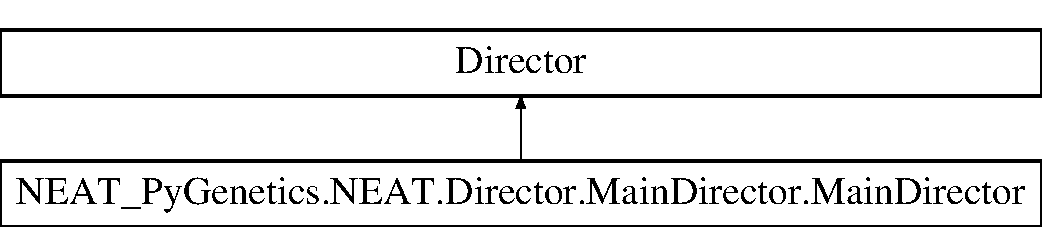
\includegraphics[height=2.000000cm]{class_n_e_a_t___py_genetics_1_1_n_e_a_t_1_1_director_1_1_main_director_1_1_main_director}
\end{center}
\end{figure}
\subsection*{Public Member Functions}
\begin{DoxyCompactItemize}
\item 
def \hyperlink{class_n_e_a_t___py_genetics_1_1_n_e_a_t_1_1_director_1_1_main_director_1_1_main_director_ab14b0501fc1b74c88b2e57f2c427f556}{\+\_\+\+\_\+init\+\_\+\+\_\+} (self, kwargs)
\item 
def \hyperlink{class_n_e_a_t___py_genetics_1_1_n_e_a_t_1_1_director_1_1_main_director_1_1_main_director_ae092b13a0703771ac0813e67fb872362}{idle} (self)
\item 
def \hyperlink{class_n_e_a_t___py_genetics_1_1_n_e_a_t_1_1_director_1_1_main_director_1_1_main_director_a145a35253c447b14b3a834cd6bbd6b15}{dynamic\+\_\+init} (self)
\item 
def {\bfseries init\+\_\+db} (self)\hypertarget{class_n_e_a_t___py_genetics_1_1_n_e_a_t_1_1_director_1_1_main_director_1_1_main_director_a1d54dab714e07b9ba097b118994bc7e0}{}\label{class_n_e_a_t___py_genetics_1_1_n_e_a_t_1_1_director_1_1_main_director_1_1_main_director_a1d54dab714e07b9ba097b118994bc7e0}

\item 
def \hyperlink{class_n_e_a_t___py_genetics_1_1_n_e_a_t_1_1_director_1_1_main_director_1_1_main_director_a0dc96b0a3075b0522e9179e154e3bfdc}{run} (self)
\item 
def \hyperlink{class_n_e_a_t___py_genetics_1_1_n_e_a_t_1_1_director_1_1_main_director_1_1_main_director_a62d21475b9a55ebf26b731e1af031998}{generate\+\_\+new\+\_\+genomes} (self)
\item 
def \hyperlink{class_n_e_a_t___py_genetics_1_1_n_e_a_t_1_1_director_1_1_main_director_1_1_main_director_a24b32672d44473d0ed697d72326a3ed0}{crossbreed\+\_\+clusters} (self)
\item 
def {\bfseries analyze\+\_\+and\+\_\+insert}\hypertarget{class_n_e_a_t___py_genetics_1_1_n_e_a_t_1_1_director_1_1_main_director_1_1_main_director_af9ec8145b3a3dc21f823d38b3ea08df1}{}\label{class_n_e_a_t___py_genetics_1_1_n_e_a_t_1_1_director_1_1_main_director_1_1_main_director_af9ec8145b3a3dc21f823d38b3ea08df1}

\item 
def \hyperlink{class_n_e_a_t___py_genetics_1_1_n_e_a_t_1_1_director_1_1_main_director_1_1_main_director_afc0fd1df30dc28284a1c9552b507298e}{calculate\+\_\+cluster\+\_\+offspring} (self)
\item 
def \hyperlink{class_n_e_a_t___py_genetics_1_1_n_e_a_t_1_1_director_1_1_main_director_1_1_main_director_a477d29aba8bdf6743748389dce049b9a}{discard\+\_\+genomes} (self)
\item 
def \hyperlink{class_n_e_a_t___py_genetics_1_1_n_e_a_t_1_1_director_1_1_main_director_1_1_main_director_a2916d65736e93f21a9a2a8f31d234615}{discard\+\_\+clusters} (self)
\item 
def {\bfseries perform\+\_\+simulation\+\_\+io} (self)\hypertarget{class_n_e_a_t___py_genetics_1_1_n_e_a_t_1_1_director_1_1_main_director_1_1_main_director_a233974c8f6d855886617f80737fb44eb}{}\label{class_n_e_a_t___py_genetics_1_1_n_e_a_t_1_1_director_1_1_main_director_1_1_main_director_a233974c8f6d855886617f80737fb44eb}

\item 
def {\bfseries compute\+\_\+genome\+\_\+outputs}\hypertarget{class_n_e_a_t___py_genetics_1_1_n_e_a_t_1_1_director_1_1_main_director_1_1_main_director_a37de122cc8ac060871f2af4da1a0a1c1}{}\label{class_n_e_a_t___py_genetics_1_1_n_e_a_t_1_1_director_1_1_main_director_1_1_main_director_a37de122cc8ac060871f2af4da1a0a1c1}

\item 
def {\bfseries update\+\_\+fitness\+\_\+values}\hypertarget{class_n_e_a_t___py_genetics_1_1_n_e_a_t_1_1_director_1_1_main_director_1_1_main_director_ab2602e228a2b8c979d4634ec21b542a8}{}\label{class_n_e_a_t___py_genetics_1_1_n_e_a_t_1_1_director_1_1_main_director_1_1_main_director_ab2602e228a2b8c979d4634ec21b542a8}

\item 
def {\bfseries init\+\_\+population} (self)\hypertarget{class_n_e_a_t___py_genetics_1_1_n_e_a_t_1_1_director_1_1_main_director_1_1_main_director_af3c8f23fba40f82bfa1a7d0b504bb218}{}\label{class_n_e_a_t___py_genetics_1_1_n_e_a_t_1_1_director_1_1_main_director_1_1_main_director_af3c8f23fba40f82bfa1a7d0b504bb218}

\end{DoxyCompactItemize}
\subsection*{Public Attributes}
\begin{DoxyCompactItemize}
\item 
{\bfseries mode}\hypertarget{class_n_e_a_t___py_genetics_1_1_n_e_a_t_1_1_director_1_1_main_director_1_1_main_director_aefb726fd87bcf69dcdfe897821481894}{}\label{class_n_e_a_t___py_genetics_1_1_n_e_a_t_1_1_director_1_1_main_director_1_1_main_director_aefb726fd87bcf69dcdfe897821481894}

\item 
{\bfseries selector}\hypertarget{class_n_e_a_t___py_genetics_1_1_n_e_a_t_1_1_director_1_1_main_director_1_1_main_director_a81175102b01b335eae3667ac36c9701f}{}\label{class_n_e_a_t___py_genetics_1_1_n_e_a_t_1_1_director_1_1_main_director_1_1_main_director_a81175102b01b335eae3667ac36c9701f}

\item 
{\bfseries decision\+\_\+maker}\hypertarget{class_n_e_a_t___py_genetics_1_1_n_e_a_t_1_1_director_1_1_main_director_1_1_main_director_accfcd32564920c4fd44a90d07e25e5c1}{}\label{class_n_e_a_t___py_genetics_1_1_n_e_a_t_1_1_director_1_1_main_director_1_1_main_director_accfcd32564920c4fd44a90d07e25e5c1}

\item 
{\bfseries breeder}\hypertarget{class_n_e_a_t___py_genetics_1_1_n_e_a_t_1_1_director_1_1_main_director_1_1_main_director_ad5b0e831f4fbc69f41056db9e477846f}{}\label{class_n_e_a_t___py_genetics_1_1_n_e_a_t_1_1_director_1_1_main_director_1_1_main_director_ad5b0e831f4fbc69f41056db9e477846f}

\item 
{\bfseries mutator}\hypertarget{class_n_e_a_t___py_genetics_1_1_n_e_a_t_1_1_director_1_1_main_director_1_1_main_director_a46ea344b5ebeead2d2d29d22ac0d3bdc}{}\label{class_n_e_a_t___py_genetics_1_1_n_e_a_t_1_1_director_1_1_main_director_1_1_main_director_a46ea344b5ebeead2d2d29d22ac0d3bdc}

\item 
{\bfseries analyst}\hypertarget{class_n_e_a_t___py_genetics_1_1_n_e_a_t_1_1_director_1_1_main_director_1_1_main_director_a2a74e9a3bfe1ee80dd5a14301d05999b}{}\label{class_n_e_a_t___py_genetics_1_1_n_e_a_t_1_1_director_1_1_main_director_1_1_main_director_a2a74e9a3bfe1ee80dd5a14301d05999b}

\item 
{\bfseries clusterer}\hypertarget{class_n_e_a_t___py_genetics_1_1_n_e_a_t_1_1_director_1_1_main_director_1_1_main_director_a9a61632f5cc72eda0e565dec59ec4956}{}\label{class_n_e_a_t___py_genetics_1_1_n_e_a_t_1_1_director_1_1_main_director_1_1_main_director_a9a61632f5cc72eda0e565dec59ec4956}

\item 
{\bfseries simulator}\hypertarget{class_n_e_a_t___py_genetics_1_1_n_e_a_t_1_1_director_1_1_main_director_1_1_main_director_a7888676faa8495bfe14559664627736d}{}\label{class_n_e_a_t___py_genetics_1_1_n_e_a_t_1_1_director_1_1_main_director_1_1_main_director_a7888676faa8495bfe14559664627736d}

\item 
{\bfseries simulation\+\_\+connector}\hypertarget{class_n_e_a_t___py_genetics_1_1_n_e_a_t_1_1_director_1_1_main_director_1_1_main_director_ab2c51deb9fa883d19a1e7c5580e60aaf}{}\label{class_n_e_a_t___py_genetics_1_1_n_e_a_t_1_1_director_1_1_main_director_1_1_main_director_ab2c51deb9fa883d19a1e7c5580e60aaf}

\item 
{\bfseries database\+\_\+connector}\hypertarget{class_n_e_a_t___py_genetics_1_1_n_e_a_t_1_1_director_1_1_main_director_1_1_main_director_a436be8b6a5893f8ade9d83a812892c35}{}\label{class_n_e_a_t___py_genetics_1_1_n_e_a_t_1_1_director_1_1_main_director_1_1_main_director_a436be8b6a5893f8ade9d83a812892c35}

\item 
{\bfseries gene\+\_\+repository}\hypertarget{class_n_e_a_t___py_genetics_1_1_n_e_a_t_1_1_director_1_1_main_director_1_1_main_director_a31df2d6f00d083b4685216a235a87ebc}{}\label{class_n_e_a_t___py_genetics_1_1_n_e_a_t_1_1_director_1_1_main_director_1_1_main_director_a31df2d6f00d083b4685216a235a87ebc}

\item 
{\bfseries genome\+\_\+repository}\hypertarget{class_n_e_a_t___py_genetics_1_1_n_e_a_t_1_1_director_1_1_main_director_1_1_main_director_a144b9b844aa917302a73065d35a9291e}{}\label{class_n_e_a_t___py_genetics_1_1_n_e_a_t_1_1_director_1_1_main_director_1_1_main_director_a144b9b844aa917302a73065d35a9291e}

\item 
{\bfseries cluster\+\_\+repository}\hypertarget{class_n_e_a_t___py_genetics_1_1_n_e_a_t_1_1_director_1_1_main_director_1_1_main_director_a96c18a6a555495afe445aadddbdcfa6f}{}\label{class_n_e_a_t___py_genetics_1_1_n_e_a_t_1_1_director_1_1_main_director_1_1_main_director_a96c18a6a555495afe445aadddbdcfa6f}

\item 
{\bfseries config}\hypertarget{class_n_e_a_t___py_genetics_1_1_n_e_a_t_1_1_director_1_1_main_director_1_1_main_director_a510d20e601183c53383179cf827ef7af}{}\label{class_n_e_a_t___py_genetics_1_1_n_e_a_t_1_1_director_1_1_main_director_1_1_main_director_a510d20e601183c53383179cf827ef7af}

\end{DoxyCompactItemize}
\subsection*{Static Public Attributes}
\begin{DoxyCompactItemize}
\item 
{\bfseries results}\hypertarget{class_n_e_a_t___py_genetics_1_1_n_e_a_t_1_1_director_1_1_main_director_1_1_main_director_acd18b971efa2d58d414e1aedcafb065d}{}\label{class_n_e_a_t___py_genetics_1_1_n_e_a_t_1_1_director_1_1_main_director_1_1_main_director_acd18b971efa2d58d414e1aedcafb065d}

\item 
{\bfseries storage\+\_\+genome}\hypertarget{class_n_e_a_t___py_genetics_1_1_n_e_a_t_1_1_director_1_1_main_director_1_1_main_director_ac579f78b49d7a2711bf925459dd1266d}{}\label{class_n_e_a_t___py_genetics_1_1_n_e_a_t_1_1_director_1_1_main_director_1_1_main_director_ac579f78b49d7a2711bf925459dd1266d}

\item 
{\bfseries outputs}\hypertarget{class_n_e_a_t___py_genetics_1_1_n_e_a_t_1_1_director_1_1_main_director_1_1_main_director_ab3116c3ed89cc021eb261dc9f3913cd2}{}\label{class_n_e_a_t___py_genetics_1_1_n_e_a_t_1_1_director_1_1_main_director_1_1_main_director_ab3116c3ed89cc021eb261dc9f3913cd2}

\end{DoxyCompactItemize}


\subsection{Detailed Description}


Definition at line 26 of file Main\+Director.\+py.



\subsection{Constructor \& Destructor Documentation}
\index{N\+E\+A\+T\+\_\+\+Py\+Genetics\+::\+N\+E\+A\+T\+::\+Director\+::\+Main\+Director\+::\+Main\+Director@{N\+E\+A\+T\+\_\+\+Py\+Genetics\+::\+N\+E\+A\+T\+::\+Director\+::\+Main\+Director\+::\+Main\+Director}!\+\_\+\+\_\+init\+\_\+\+\_\+@{\+\_\+\+\_\+init\+\_\+\+\_\+}}
\index{\+\_\+\+\_\+init\+\_\+\+\_\+@{\+\_\+\+\_\+init\+\_\+\+\_\+}!N\+E\+A\+T\+\_\+\+Py\+Genetics\+::\+N\+E\+A\+T\+::\+Director\+::\+Main\+Director\+::\+Main\+Director@{N\+E\+A\+T\+\_\+\+Py\+Genetics\+::\+N\+E\+A\+T\+::\+Director\+::\+Main\+Director\+::\+Main\+Director}}
\subsubsection[{\texorpdfstring{\+\_\+\+\_\+init\+\_\+\+\_\+(self, kwargs)}{__init__(self, kwargs)}}]{\setlength{\rightskip}{0pt plus 5cm}def N\+E\+A\+T\+\_\+\+Py\+Genetics.\+N\+E\+A\+T.\+Director.\+Main\+Director.\+Main\+Director.\+\_\+\+\_\+init\+\_\+\+\_\+ (
\begin{DoxyParamCaption}
\item[{}]{self, }
\item[{}]{kwargs}
\end{DoxyParamCaption}
)}\hypertarget{class_n_e_a_t___py_genetics_1_1_n_e_a_t_1_1_director_1_1_main_director_1_1_main_director_ab14b0501fc1b74c88b2e57f2c427f556}{}\label{class_n_e_a_t___py_genetics_1_1_n_e_a_t_1_1_director_1_1_main_director_1_1_main_director_ab14b0501fc1b74c88b2e57f2c427f556}
\begin{DoxyVerb}:param kwargs:
    - mode:
- exit: exits the program, default action if nothing is provided.
- new: creates a new database for a given simulation. requires parame-
 ter simulation to be set.
- load: loads a database for a given simulation. requires parameter
 simulation to be set.
    - simulation: the name of the simulation that should be used. must cor-
      respond to a module name in Simulation.
:return:
\end{DoxyVerb}
 

Definition at line 27 of file Main\+Director.\+py.



\subsection{Member Function Documentation}
\index{N\+E\+A\+T\+\_\+\+Py\+Genetics\+::\+N\+E\+A\+T\+::\+Director\+::\+Main\+Director\+::\+Main\+Director@{N\+E\+A\+T\+\_\+\+Py\+Genetics\+::\+N\+E\+A\+T\+::\+Director\+::\+Main\+Director\+::\+Main\+Director}!calculate\+\_\+cluster\+\_\+offspring@{calculate\+\_\+cluster\+\_\+offspring}}
\index{calculate\+\_\+cluster\+\_\+offspring@{calculate\+\_\+cluster\+\_\+offspring}!N\+E\+A\+T\+\_\+\+Py\+Genetics\+::\+N\+E\+A\+T\+::\+Director\+::\+Main\+Director\+::\+Main\+Director@{N\+E\+A\+T\+\_\+\+Py\+Genetics\+::\+N\+E\+A\+T\+::\+Director\+::\+Main\+Director\+::\+Main\+Director}}
\subsubsection[{\texorpdfstring{calculate\+\_\+cluster\+\_\+offspring(self)}{calculate_cluster_offspring(self)}}]{\setlength{\rightskip}{0pt plus 5cm}def N\+E\+A\+T\+\_\+\+Py\+Genetics.\+N\+E\+A\+T.\+Director.\+Main\+Director.\+Main\+Director.\+calculate\+\_\+cluster\+\_\+offspring (
\begin{DoxyParamCaption}
\item[{}]{self}
\end{DoxyParamCaption}
)}\hypertarget{class_n_e_a_t___py_genetics_1_1_n_e_a_t_1_1_director_1_1_main_director_1_1_main_director_afc0fd1df30dc28284a1c9552b507298e}{}\label{class_n_e_a_t___py_genetics_1_1_n_e_a_t_1_1_director_1_1_main_director_1_1_main_director_afc0fd1df30dc28284a1c9552b507298e}
\begin{DoxyVerb}Calculates fitness values and offspring for clusters.
:return:
\end{DoxyVerb}
 

Definition at line 275 of file Main\+Director.\+py.

\index{N\+E\+A\+T\+\_\+\+Py\+Genetics\+::\+N\+E\+A\+T\+::\+Director\+::\+Main\+Director\+::\+Main\+Director@{N\+E\+A\+T\+\_\+\+Py\+Genetics\+::\+N\+E\+A\+T\+::\+Director\+::\+Main\+Director\+::\+Main\+Director}!crossbreed\+\_\+clusters@{crossbreed\+\_\+clusters}}
\index{crossbreed\+\_\+clusters@{crossbreed\+\_\+clusters}!N\+E\+A\+T\+\_\+\+Py\+Genetics\+::\+N\+E\+A\+T\+::\+Director\+::\+Main\+Director\+::\+Main\+Director@{N\+E\+A\+T\+\_\+\+Py\+Genetics\+::\+N\+E\+A\+T\+::\+Director\+::\+Main\+Director\+::\+Main\+Director}}
\subsubsection[{\texorpdfstring{crossbreed\+\_\+clusters(self)}{crossbreed_clusters(self)}}]{\setlength{\rightskip}{0pt plus 5cm}def N\+E\+A\+T\+\_\+\+Py\+Genetics.\+N\+E\+A\+T.\+Director.\+Main\+Director.\+Main\+Director.\+crossbreed\+\_\+clusters (
\begin{DoxyParamCaption}
\item[{}]{self}
\end{DoxyParamCaption}
)}\hypertarget{class_n_e_a_t___py_genetics_1_1_n_e_a_t_1_1_director_1_1_main_director_1_1_main_director_a24b32672d44473d0ed697d72326a3ed0}{}\label{class_n_e_a_t___py_genetics_1_1_n_e_a_t_1_1_director_1_1_main_director_1_1_main_director_a24b32672d44473d0ed697d72326a3ed0}
\begin{DoxyVerb}combines two clusters by breeding genomes of both clusters
:return:
\end{DoxyVerb}
 

Definition at line 251 of file Main\+Director.\+py.

\index{N\+E\+A\+T\+\_\+\+Py\+Genetics\+::\+N\+E\+A\+T\+::\+Director\+::\+Main\+Director\+::\+Main\+Director@{N\+E\+A\+T\+\_\+\+Py\+Genetics\+::\+N\+E\+A\+T\+::\+Director\+::\+Main\+Director\+::\+Main\+Director}!discard\+\_\+clusters@{discard\+\_\+clusters}}
\index{discard\+\_\+clusters@{discard\+\_\+clusters}!N\+E\+A\+T\+\_\+\+Py\+Genetics\+::\+N\+E\+A\+T\+::\+Director\+::\+Main\+Director\+::\+Main\+Director@{N\+E\+A\+T\+\_\+\+Py\+Genetics\+::\+N\+E\+A\+T\+::\+Director\+::\+Main\+Director\+::\+Main\+Director}}
\subsubsection[{\texorpdfstring{discard\+\_\+clusters(self)}{discard_clusters(self)}}]{\setlength{\rightskip}{0pt plus 5cm}def N\+E\+A\+T\+\_\+\+Py\+Genetics.\+N\+E\+A\+T.\+Director.\+Main\+Director.\+Main\+Director.\+discard\+\_\+clusters (
\begin{DoxyParamCaption}
\item[{}]{self}
\end{DoxyParamCaption}
)}\hypertarget{class_n_e_a_t___py_genetics_1_1_n_e_a_t_1_1_director_1_1_main_director_1_1_main_director_a2916d65736e93f21a9a2a8f31d234615}{}\label{class_n_e_a_t___py_genetics_1_1_n_e_a_t_1_1_director_1_1_main_director_1_1_main_director_a2916d65736e93f21a9a2a8f31d234615}
\begin{DoxyVerb}Discards a number of clusters
:return:
\end{DoxyVerb}
 

Definition at line 290 of file Main\+Director.\+py.

\index{N\+E\+A\+T\+\_\+\+Py\+Genetics\+::\+N\+E\+A\+T\+::\+Director\+::\+Main\+Director\+::\+Main\+Director@{N\+E\+A\+T\+\_\+\+Py\+Genetics\+::\+N\+E\+A\+T\+::\+Director\+::\+Main\+Director\+::\+Main\+Director}!discard\+\_\+genomes@{discard\+\_\+genomes}}
\index{discard\+\_\+genomes@{discard\+\_\+genomes}!N\+E\+A\+T\+\_\+\+Py\+Genetics\+::\+N\+E\+A\+T\+::\+Director\+::\+Main\+Director\+::\+Main\+Director@{N\+E\+A\+T\+\_\+\+Py\+Genetics\+::\+N\+E\+A\+T\+::\+Director\+::\+Main\+Director\+::\+Main\+Director}}
\subsubsection[{\texorpdfstring{discard\+\_\+genomes(self)}{discard_genomes(self)}}]{\setlength{\rightskip}{0pt plus 5cm}def N\+E\+A\+T\+\_\+\+Py\+Genetics.\+N\+E\+A\+T.\+Director.\+Main\+Director.\+Main\+Director.\+discard\+\_\+genomes (
\begin{DoxyParamCaption}
\item[{}]{self}
\end{DoxyParamCaption}
)}\hypertarget{class_n_e_a_t___py_genetics_1_1_n_e_a_t_1_1_director_1_1_main_director_1_1_main_director_a477d29aba8bdf6743748389dce049b9a}{}\label{class_n_e_a_t___py_genetics_1_1_n_e_a_t_1_1_director_1_1_main_director_1_1_main_director_a477d29aba8bdf6743748389dce049b9a}
\begin{DoxyVerb}discards a number of genomes
:return:
\end{DoxyVerb}
 

Definition at line 282 of file Main\+Director.\+py.

\index{N\+E\+A\+T\+\_\+\+Py\+Genetics\+::\+N\+E\+A\+T\+::\+Director\+::\+Main\+Director\+::\+Main\+Director@{N\+E\+A\+T\+\_\+\+Py\+Genetics\+::\+N\+E\+A\+T\+::\+Director\+::\+Main\+Director\+::\+Main\+Director}!dynamic\+\_\+init@{dynamic\+\_\+init}}
\index{dynamic\+\_\+init@{dynamic\+\_\+init}!N\+E\+A\+T\+\_\+\+Py\+Genetics\+::\+N\+E\+A\+T\+::\+Director\+::\+Main\+Director\+::\+Main\+Director@{N\+E\+A\+T\+\_\+\+Py\+Genetics\+::\+N\+E\+A\+T\+::\+Director\+::\+Main\+Director\+::\+Main\+Director}}
\subsubsection[{\texorpdfstring{dynamic\+\_\+init(self)}{dynamic_init(self)}}]{\setlength{\rightskip}{0pt plus 5cm}def N\+E\+A\+T\+\_\+\+Py\+Genetics.\+N\+E\+A\+T.\+Director.\+Main\+Director.\+Main\+Director.\+dynamic\+\_\+init (
\begin{DoxyParamCaption}
\item[{}]{self}
\end{DoxyParamCaption}
)}\hypertarget{class_n_e_a_t___py_genetics_1_1_n_e_a_t_1_1_director_1_1_main_director_1_1_main_director_a145a35253c447b14b3a834cd6bbd6b15}{}\label{class_n_e_a_t___py_genetics_1_1_n_e_a_t_1_1_director_1_1_main_director_1_1_main_director_a145a35253c447b14b3a834cd6bbd6b15}
\begin{DoxyVerb}Initializes all parts of NEAT that are dependent upon
the client.
\end{DoxyVerb}
 

Definition at line 91 of file Main\+Director.\+py.

\index{N\+E\+A\+T\+\_\+\+Py\+Genetics\+::\+N\+E\+A\+T\+::\+Director\+::\+Main\+Director\+::\+Main\+Director@{N\+E\+A\+T\+\_\+\+Py\+Genetics\+::\+N\+E\+A\+T\+::\+Director\+::\+Main\+Director\+::\+Main\+Director}!generate\+\_\+new\+\_\+genomes@{generate\+\_\+new\+\_\+genomes}}
\index{generate\+\_\+new\+\_\+genomes@{generate\+\_\+new\+\_\+genomes}!N\+E\+A\+T\+\_\+\+Py\+Genetics\+::\+N\+E\+A\+T\+::\+Director\+::\+Main\+Director\+::\+Main\+Director@{N\+E\+A\+T\+\_\+\+Py\+Genetics\+::\+N\+E\+A\+T\+::\+Director\+::\+Main\+Director\+::\+Main\+Director}}
\subsubsection[{\texorpdfstring{generate\+\_\+new\+\_\+genomes(self)}{generate_new_genomes(self)}}]{\setlength{\rightskip}{0pt plus 5cm}def N\+E\+A\+T\+\_\+\+Py\+Genetics.\+N\+E\+A\+T.\+Director.\+Main\+Director.\+Main\+Director.\+generate\+\_\+new\+\_\+genomes (
\begin{DoxyParamCaption}
\item[{}]{self}
\end{DoxyParamCaption}
)}\hypertarget{class_n_e_a_t___py_genetics_1_1_n_e_a_t_1_1_director_1_1_main_director_1_1_main_director_a62d21475b9a55ebf26b731e1af031998}{}\label{class_n_e_a_t___py_genetics_1_1_n_e_a_t_1_1_director_1_1_main_director_1_1_main_director_a62d21475b9a55ebf26b731e1af031998}
\begin{DoxyVerb}Regenerates the population by selecting genomes for
mutation / breeding, running the generation process and performing analysis.
:return:
\end{DoxyVerb}
 

Definition at line 225 of file Main\+Director.\+py.

\index{N\+E\+A\+T\+\_\+\+Py\+Genetics\+::\+N\+E\+A\+T\+::\+Director\+::\+Main\+Director\+::\+Main\+Director@{N\+E\+A\+T\+\_\+\+Py\+Genetics\+::\+N\+E\+A\+T\+::\+Director\+::\+Main\+Director\+::\+Main\+Director}!idle@{idle}}
\index{idle@{idle}!N\+E\+A\+T\+\_\+\+Py\+Genetics\+::\+N\+E\+A\+T\+::\+Director\+::\+Main\+Director\+::\+Main\+Director@{N\+E\+A\+T\+\_\+\+Py\+Genetics\+::\+N\+E\+A\+T\+::\+Director\+::\+Main\+Director\+::\+Main\+Director}}
\subsubsection[{\texorpdfstring{idle(self)}{idle(self)}}]{\setlength{\rightskip}{0pt plus 5cm}def N\+E\+A\+T\+\_\+\+Py\+Genetics.\+N\+E\+A\+T.\+Director.\+Main\+Director.\+Main\+Director.\+idle (
\begin{DoxyParamCaption}
\item[{}]{self}
\end{DoxyParamCaption}
)}\hypertarget{class_n_e_a_t___py_genetics_1_1_n_e_a_t_1_1_director_1_1_main_director_1_1_main_director_ae092b13a0703771ac0813e67fb872362}{}\label{class_n_e_a_t___py_genetics_1_1_n_e_a_t_1_1_director_1_1_main_director_1_1_main_director_ae092b13a0703771ac0813e67fb872362}
\begin{DoxyVerb}Standard method that will be executed if local startup is done.
In this state, the Director will wait for the client.
\end{DoxyVerb}
 

Definition at line 72 of file Main\+Director.\+py.

\index{N\+E\+A\+T\+\_\+\+Py\+Genetics\+::\+N\+E\+A\+T\+::\+Director\+::\+Main\+Director\+::\+Main\+Director@{N\+E\+A\+T\+\_\+\+Py\+Genetics\+::\+N\+E\+A\+T\+::\+Director\+::\+Main\+Director\+::\+Main\+Director}!run@{run}}
\index{run@{run}!N\+E\+A\+T\+\_\+\+Py\+Genetics\+::\+N\+E\+A\+T\+::\+Director\+::\+Main\+Director\+::\+Main\+Director@{N\+E\+A\+T\+\_\+\+Py\+Genetics\+::\+N\+E\+A\+T\+::\+Director\+::\+Main\+Director\+::\+Main\+Director}}
\subsubsection[{\texorpdfstring{run(self)}{run(self)}}]{\setlength{\rightskip}{0pt plus 5cm}def N\+E\+A\+T\+\_\+\+Py\+Genetics.\+N\+E\+A\+T.\+Director.\+Main\+Director.\+Main\+Director.\+run (
\begin{DoxyParamCaption}
\item[{}]{self}
\end{DoxyParamCaption}
)}\hypertarget{class_n_e_a_t___py_genetics_1_1_n_e_a_t_1_1_director_1_1_main_director_1_1_main_director_a0dc96b0a3075b0522e9179e154e3bfdc}{}\label{class_n_e_a_t___py_genetics_1_1_n_e_a_t_1_1_director_1_1_main_director_1_1_main_director_a0dc96b0a3075b0522e9179e154e3bfdc}
\begin{DoxyVerb}The main function where the simulation is run, new
genomes are created and discarded
This is where the evolutionary magic happens.
\end{DoxyVerb}
 

Definition at line 167 of file Main\+Director.\+py.



The documentation for this class was generated from the following file\+:\begin{DoxyCompactItemize}
\item 
N\+E\+A\+T/\+Director/Main\+Director.\+py\end{DoxyCompactItemize}

\hypertarget{class_n_e_a_t___py_genetics_1_1_n_e_a_t_1_1_tests_1_1_mock_classes_1_1mock___cluster_repository_1_1mock___cluster_repository}{}\section{N\+E\+A\+T\+\_\+\+Py\+Genetics.\+N\+E\+A\+T.\+Tests.\+Mock\+Classes.\+mock\+\_\+\+Cluster\+Repository.\+mock\+\_\+\+Cluster\+Repository Class Reference}
\label{class_n_e_a_t___py_genetics_1_1_n_e_a_t_1_1_tests_1_1_mock_classes_1_1mock___cluster_repository_1_1mock___cluster_repository}\index{N\+E\+A\+T\+\_\+\+Py\+Genetics.\+N\+E\+A\+T.\+Tests.\+Mock\+Classes.\+mock\+\_\+\+Cluster\+Repository.\+mock\+\_\+\+Cluster\+Repository@{N\+E\+A\+T\+\_\+\+Py\+Genetics.\+N\+E\+A\+T.\+Tests.\+Mock\+Classes.\+mock\+\_\+\+Cluster\+Repository.\+mock\+\_\+\+Cluster\+Repository}}
Inheritance diagram for N\+E\+A\+T\+\_\+\+Py\+Genetics.\+N\+E\+A\+T.\+Tests.\+Mock\+Classes.\+mock\+\_\+\+Cluster\+Repository.\+mock\+\_\+\+Cluster\+Repository\+:\begin{figure}[H]
\begin{center}
\leavevmode
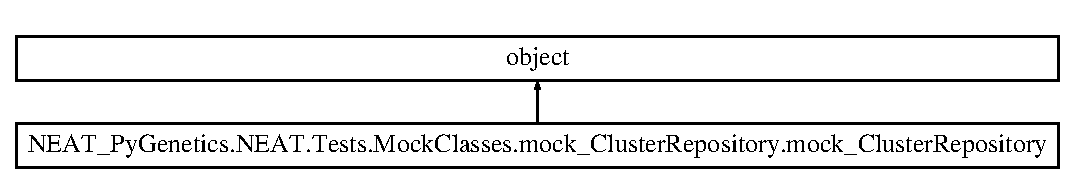
\includegraphics[height=2.000000cm]{class_n_e_a_t___py_genetics_1_1_n_e_a_t_1_1_tests_1_1_mock_classes_1_1mock___cluster_repository_1_1mock___cluster_repository}
\end{center}
\end{figure}
\subsection*{Public Member Functions}
\begin{DoxyCompactItemize}
\item 
def {\bfseries \+\_\+\+\_\+init\+\_\+\+\_\+} (self)\hypertarget{class_n_e_a_t___py_genetics_1_1_n_e_a_t_1_1_tests_1_1_mock_classes_1_1mock___cluster_repository_1_1mock___cluster_repository_a9f89fd3f00cd01d78dcae1af7b061c8a}{}\label{class_n_e_a_t___py_genetics_1_1_n_e_a_t_1_1_tests_1_1_mock_classes_1_1mock___cluster_repository_1_1mock___cluster_repository_a9f89fd3f00cd01d78dcae1af7b061c8a}

\item 
def {\bfseries reset} (self)\hypertarget{class_n_e_a_t___py_genetics_1_1_n_e_a_t_1_1_tests_1_1_mock_classes_1_1mock___cluster_repository_1_1mock___cluster_repository_a7c1d0e1494945daece920c3faa393417}{}\label{class_n_e_a_t___py_genetics_1_1_n_e_a_t_1_1_tests_1_1_mock_classes_1_1mock___cluster_repository_1_1mock___cluster_repository_a7c1d0e1494945daece920c3faa393417}

\item 
def {\bfseries get\+\_\+cluster\+\_\+count} (self)\hypertarget{class_n_e_a_t___py_genetics_1_1_n_e_a_t_1_1_tests_1_1_mock_classes_1_1mock___cluster_repository_1_1mock___cluster_repository_aaedaee0f127d37e0c3a5521f15364277}{}\label{class_n_e_a_t___py_genetics_1_1_n_e_a_t_1_1_tests_1_1_mock_classes_1_1mock___cluster_repository_1_1mock___cluster_repository_aaedaee0f127d37e0c3a5521f15364277}

\item 
def {\bfseries add\+\_\+cluster\+\_\+with\+\_\+representative}\hypertarget{class_n_e_a_t___py_genetics_1_1_n_e_a_t_1_1_tests_1_1_mock_classes_1_1mock___cluster_repository_1_1mock___cluster_repository_a226b6c12fc2b76219c55c9e4b99baa16}{}\label{class_n_e_a_t___py_genetics_1_1_n_e_a_t_1_1_tests_1_1_mock_classes_1_1mock___cluster_repository_1_1mock___cluster_repository_a226b6c12fc2b76219c55c9e4b99baa16}

\item 
def {\bfseries get\+\_\+current\+\_\+clusters} (self)\hypertarget{class_n_e_a_t___py_genetics_1_1_n_e_a_t_1_1_tests_1_1_mock_classes_1_1mock___cluster_repository_1_1mock___cluster_repository_a134f5b068a5237328c7c3b481852bafd}{}\label{class_n_e_a_t___py_genetics_1_1_n_e_a_t_1_1_tests_1_1_mock_classes_1_1mock___cluster_repository_1_1mock___cluster_repository_a134f5b068a5237328c7c3b481852bafd}

\item 
def {\bfseries get\+\_\+cluster\+\_\+by\+\_\+representative}\hypertarget{class_n_e_a_t___py_genetics_1_1_n_e_a_t_1_1_tests_1_1_mock_classes_1_1mock___cluster_repository_1_1mock___cluster_repository_abeb34604f2a2aa59c79c0db965494929}{}\label{class_n_e_a_t___py_genetics_1_1_n_e_a_t_1_1_tests_1_1_mock_classes_1_1mock___cluster_repository_1_1mock___cluster_repository_abeb34604f2a2aa59c79c0db965494929}

\item 
def {\bfseries update\+\_\+fitness\+\_\+for\+\_\+cluster}\hypertarget{class_n_e_a_t___py_genetics_1_1_n_e_a_t_1_1_tests_1_1_mock_classes_1_1mock___cluster_repository_1_1mock___cluster_repository_aee0e3e9834f04db0768aefa4949fecdf}{}\label{class_n_e_a_t___py_genetics_1_1_n_e_a_t_1_1_tests_1_1_mock_classes_1_1mock___cluster_repository_1_1mock___cluster_repository_aee0e3e9834f04db0768aefa4949fecdf}

\item 
def {\bfseries update\+\_\+max\+\_\+population\+\_\+for\+\_\+cluster}\hypertarget{class_n_e_a_t___py_genetics_1_1_n_e_a_t_1_1_tests_1_1_mock_classes_1_1mock___cluster_repository_1_1mock___cluster_repository_a750492b84023bed8ca6f78ccda904de5}{}\label{class_n_e_a_t___py_genetics_1_1_n_e_a_t_1_1_tests_1_1_mock_classes_1_1mock___cluster_repository_1_1mock___cluster_repository_a750492b84023bed8ca6f78ccda904de5}

\item 
def {\bfseries update\+\_\+offspring\+\_\+for\+\_\+cluster}\hypertarget{class_n_e_a_t___py_genetics_1_1_n_e_a_t_1_1_tests_1_1_mock_classes_1_1mock___cluster_repository_1_1mock___cluster_repository_ac6f8854ca405235c472100f1b9519762}{}\label{class_n_e_a_t___py_genetics_1_1_n_e_a_t_1_1_tests_1_1_mock_classes_1_1mock___cluster_repository_1_1mock___cluster_repository_ac6f8854ca405235c472100f1b9519762}

\end{DoxyCompactItemize}
\subsection*{Public Attributes}
\begin{DoxyCompactItemize}
\item 
{\bfseries clusters}\hypertarget{class_n_e_a_t___py_genetics_1_1_n_e_a_t_1_1_tests_1_1_mock_classes_1_1mock___cluster_repository_1_1mock___cluster_repository_a2e2d77ba5375cceedf179e25c7887de5}{}\label{class_n_e_a_t___py_genetics_1_1_n_e_a_t_1_1_tests_1_1_mock_classes_1_1mock___cluster_repository_1_1mock___cluster_repository_a2e2d77ba5375cceedf179e25c7887de5}

\item 
{\bfseries next\+\_\+id}\hypertarget{class_n_e_a_t___py_genetics_1_1_n_e_a_t_1_1_tests_1_1_mock_classes_1_1mock___cluster_repository_1_1mock___cluster_repository_a3b7a06a95cca18e535ce14621cd4fa4d}{}\label{class_n_e_a_t___py_genetics_1_1_n_e_a_t_1_1_tests_1_1_mock_classes_1_1mock___cluster_repository_1_1mock___cluster_repository_a3b7a06a95cca18e535ce14621cd4fa4d}

\end{DoxyCompactItemize}


\subsection{Detailed Description}


Definition at line 5 of file mock\+\_\+\+Cluster\+Repository.\+py.



The documentation for this class was generated from the following file\+:\begin{DoxyCompactItemize}
\item 
N\+E\+A\+T/\+Tests/\+Mock\+Classes/mock\+\_\+\+Cluster\+Repository.\+py\end{DoxyCompactItemize}

\hypertarget{class_n_e_a_t___py_genetics_1_1_n_e_a_t_1_1_tests_1_1_mock_classes_1_1mock___database_connector_1_1mock___database_connector}{}\section{N\+E\+A\+T\+\_\+\+Py\+Genetics.\+N\+E\+A\+T.\+Tests.\+Mock\+Classes.\+mock\+\_\+\+Database\+Connector.\+mock\+\_\+\+Database\+Connector Class Reference}
\label{class_n_e_a_t___py_genetics_1_1_n_e_a_t_1_1_tests_1_1_mock_classes_1_1mock___database_connector_1_1mock___database_connector}\index{N\+E\+A\+T\+\_\+\+Py\+Genetics.\+N\+E\+A\+T.\+Tests.\+Mock\+Classes.\+mock\+\_\+\+Database\+Connector.\+mock\+\_\+\+Database\+Connector@{N\+E\+A\+T\+\_\+\+Py\+Genetics.\+N\+E\+A\+T.\+Tests.\+Mock\+Classes.\+mock\+\_\+\+Database\+Connector.\+mock\+\_\+\+Database\+Connector}}
Inheritance diagram for N\+E\+A\+T\+\_\+\+Py\+Genetics.\+N\+E\+A\+T.\+Tests.\+Mock\+Classes.\+mock\+\_\+\+Database\+Connector.\+mock\+\_\+\+Database\+Connector\+:\begin{figure}[H]
\begin{center}
\leavevmode
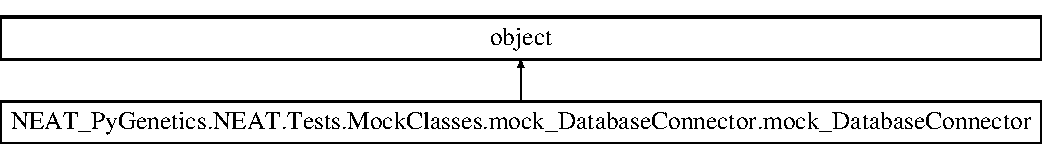
\includegraphics[height=1.941074cm]{class_n_e_a_t___py_genetics_1_1_n_e_a_t_1_1_tests_1_1_mock_classes_1_1mock___database_connector_1_1mock___database_connector}
\end{center}
\end{figure}
\subsection*{Public Member Functions}
\begin{DoxyCompactItemize}
\item 
def {\bfseries \+\_\+\+\_\+init\+\_\+\+\_\+} (self)\hypertarget{class_n_e_a_t___py_genetics_1_1_n_e_a_t_1_1_tests_1_1_mock_classes_1_1mock___database_connector_1_1mock___database_connector_a02398d61ab2bab01e548b901cd4d70f7}{}\label{class_n_e_a_t___py_genetics_1_1_n_e_a_t_1_1_tests_1_1_mock_classes_1_1mock___database_connector_1_1mock___database_connector_a02398d61ab2bab01e548b901cd4d70f7}

\item 
def {\bfseries get\+\_\+collection}\hypertarget{class_n_e_a_t___py_genetics_1_1_n_e_a_t_1_1_tests_1_1_mock_classes_1_1mock___database_connector_1_1mock___database_connector_aef1a53517f1680bcc5ddfcbeff3f4785}{}\label{class_n_e_a_t___py_genetics_1_1_n_e_a_t_1_1_tests_1_1_mock_classes_1_1mock___database_connector_1_1mock___database_connector_aef1a53517f1680bcc5ddfcbeff3f4785}

\item 
def {\bfseries insert\+\_\+one}\hypertarget{class_n_e_a_t___py_genetics_1_1_n_e_a_t_1_1_tests_1_1_mock_classes_1_1mock___database_connector_1_1mock___database_connector_a9f8c8a2adf0987729548df63dfe118e8}{}\label{class_n_e_a_t___py_genetics_1_1_n_e_a_t_1_1_tests_1_1_mock_classes_1_1mock___database_connector_1_1mock___database_connector_a9f8c8a2adf0987729548df63dfe118e8}

\item 
def {\bfseries insert\+\_\+many}\hypertarget{class_n_e_a_t___py_genetics_1_1_n_e_a_t_1_1_tests_1_1_mock_classes_1_1mock___database_connector_1_1mock___database_connector_a0c7202b51bd1bf1001d3748ac39d825b}{}\label{class_n_e_a_t___py_genetics_1_1_n_e_a_t_1_1_tests_1_1_mock_classes_1_1mock___database_connector_1_1mock___database_connector_a0c7202b51bd1bf1001d3748ac39d825b}

\item 
def {\bfseries find\+\_\+one}\hypertarget{class_n_e_a_t___py_genetics_1_1_n_e_a_t_1_1_tests_1_1_mock_classes_1_1mock___database_connector_1_1mock___database_connector_ac03ab8b0c7fda497eac3ca7435aec3a0}{}\label{class_n_e_a_t___py_genetics_1_1_n_e_a_t_1_1_tests_1_1_mock_classes_1_1mock___database_connector_1_1mock___database_connector_ac03ab8b0c7fda497eac3ca7435aec3a0}

\item 
def {\bfseries find\+\_\+one\+\_\+by\+\_\+id}\hypertarget{class_n_e_a_t___py_genetics_1_1_n_e_a_t_1_1_tests_1_1_mock_classes_1_1mock___database_connector_1_1mock___database_connector_ace6331811ba2e674ef037a66d073377a}{}\label{class_n_e_a_t___py_genetics_1_1_n_e_a_t_1_1_tests_1_1_mock_classes_1_1mock___database_connector_1_1mock___database_connector_ace6331811ba2e674ef037a66d073377a}

\item 
def {\bfseries find\+\_\+many}\hypertarget{class_n_e_a_t___py_genetics_1_1_n_e_a_t_1_1_tests_1_1_mock_classes_1_1mock___database_connector_1_1mock___database_connector_a0ea2557b31cd7af3af9e098cc8dd3f7d}{}\label{class_n_e_a_t___py_genetics_1_1_n_e_a_t_1_1_tests_1_1_mock_classes_1_1mock___database_connector_1_1mock___database_connector_a0ea2557b31cd7af3af9e098cc8dd3f7d}

\item 
def {\bfseries update\+\_\+one}\hypertarget{class_n_e_a_t___py_genetics_1_1_n_e_a_t_1_1_tests_1_1_mock_classes_1_1mock___database_connector_1_1mock___database_connector_a01f612634b7f3da00fb1b327dfa5b524}{}\label{class_n_e_a_t___py_genetics_1_1_n_e_a_t_1_1_tests_1_1_mock_classes_1_1mock___database_connector_1_1mock___database_connector_a01f612634b7f3da00fb1b327dfa5b524}

\item 
def {\bfseries update\+\_\+many}\hypertarget{class_n_e_a_t___py_genetics_1_1_n_e_a_t_1_1_tests_1_1_mock_classes_1_1mock___database_connector_1_1mock___database_connector_a9fa32e7c0e425396238b66ab8f3ffb5e}{}\label{class_n_e_a_t___py_genetics_1_1_n_e_a_t_1_1_tests_1_1_mock_classes_1_1mock___database_connector_1_1mock___database_connector_a9fa32e7c0e425396238b66ab8f3ffb5e}

\item 
def {\bfseries remove\+\_\+one}\hypertarget{class_n_e_a_t___py_genetics_1_1_n_e_a_t_1_1_tests_1_1_mock_classes_1_1mock___database_connector_1_1mock___database_connector_a534ae334b83f54bce7d32f66faf22440}{}\label{class_n_e_a_t___py_genetics_1_1_n_e_a_t_1_1_tests_1_1_mock_classes_1_1mock___database_connector_1_1mock___database_connector_a534ae334b83f54bce7d32f66faf22440}

\item 
def {\bfseries remove\+\_\+many}\hypertarget{class_n_e_a_t___py_genetics_1_1_n_e_a_t_1_1_tests_1_1_mock_classes_1_1mock___database_connector_1_1mock___database_connector_ab3ff82b4de49e912a56c7b3cd0a208ac}{}\label{class_n_e_a_t___py_genetics_1_1_n_e_a_t_1_1_tests_1_1_mock_classes_1_1mock___database_connector_1_1mock___database_connector_ab3ff82b4de49e912a56c7b3cd0a208ac}

\item 
def {\bfseries create\+\_\+collection\+\_\+if\+\_\+not\+\_\+exists} (self, collection\+\_\+name)\hypertarget{class_n_e_a_t___py_genetics_1_1_n_e_a_t_1_1_tests_1_1_mock_classes_1_1mock___database_connector_1_1mock___database_connector_a9092111a34ce0573dace98120682e415}{}\label{class_n_e_a_t___py_genetics_1_1_n_e_a_t_1_1_tests_1_1_mock_classes_1_1mock___database_connector_1_1mock___database_connector_a9092111a34ce0573dace98120682e415}

\item 
def {\bfseries next\+\_\+id} (self)\hypertarget{class_n_e_a_t___py_genetics_1_1_n_e_a_t_1_1_tests_1_1_mock_classes_1_1mock___database_connector_1_1mock___database_connector_a7172e251a453e9481d7c8359b6961105}{}\label{class_n_e_a_t___py_genetics_1_1_n_e_a_t_1_1_tests_1_1_mock_classes_1_1mock___database_connector_1_1mock___database_connector_a7172e251a453e9481d7c8359b6961105}

\end{DoxyCompactItemize}
\subsection*{Static Public Attributes}
\begin{DoxyCompactItemize}
\item 
{\bfseries assigned\+\_\+id}\hypertarget{class_n_e_a_t___py_genetics_1_1_n_e_a_t_1_1_tests_1_1_mock_classes_1_1mock___database_connector_1_1mock___database_connector_aaa8b3d15b7e01aef04c5ab3f58e8a006}{}\label{class_n_e_a_t___py_genetics_1_1_n_e_a_t_1_1_tests_1_1_mock_classes_1_1mock___database_connector_1_1mock___database_connector_aaa8b3d15b7e01aef04c5ab3f58e8a006}

\item 
{\bfseries assigned\+\_\+ids}\hypertarget{class_n_e_a_t___py_genetics_1_1_n_e_a_t_1_1_tests_1_1_mock_classes_1_1mock___database_connector_1_1mock___database_connector_a6061ac8abee52f8e6d81b92c24c944eb}{}\label{class_n_e_a_t___py_genetics_1_1_n_e_a_t_1_1_tests_1_1_mock_classes_1_1mock___database_connector_1_1mock___database_connector_a6061ac8abee52f8e6d81b92c24c944eb}

\item 
{\bfseries filter\+\_\+mismatch}\hypertarget{class_n_e_a_t___py_genetics_1_1_n_e_a_t_1_1_tests_1_1_mock_classes_1_1mock___database_connector_1_1mock___database_connector_a7e65d11937c1858690f2cd25ac07de18}{}\label{class_n_e_a_t___py_genetics_1_1_n_e_a_t_1_1_tests_1_1_mock_classes_1_1mock___database_connector_1_1mock___database_connector_a7e65d11937c1858690f2cd25ac07de18}

\item 
{\bfseries results}\hypertarget{class_n_e_a_t___py_genetics_1_1_n_e_a_t_1_1_tests_1_1_mock_classes_1_1mock___database_connector_1_1mock___database_connector_a3370fecdccb2abc0c0a3356825f04cc4}{}\label{class_n_e_a_t___py_genetics_1_1_n_e_a_t_1_1_tests_1_1_mock_classes_1_1mock___database_connector_1_1mock___database_connector_a3370fecdccb2abc0c0a3356825f04cc4}

\end{DoxyCompactItemize}


\subsection{Detailed Description}


Definition at line 3 of file mock\+\_\+\+Database\+Connector.\+py.



The documentation for this class was generated from the following file\+:\begin{DoxyCompactItemize}
\item 
N\+E\+A\+T/\+Tests/\+Mock\+Classes/mock\+\_\+\+Database\+Connector.\+py\end{DoxyCompactItemize}

\hypertarget{class_n_e_a_t___py_genetics_1_1_n_e_a_t_1_1_tests_1_1_mock_classes_1_1mock___gene_repository_1_1mock___gene_repository}{}\section{N\+E\+A\+T\+\_\+\+Py\+Genetics.\+N\+E\+A\+T.\+Tests.\+Mock\+Classes.\+mock\+\_\+\+Gene\+Repository.\+mock\+\_\+\+Gene\+Repository Class Reference}
\label{class_n_e_a_t___py_genetics_1_1_n_e_a_t_1_1_tests_1_1_mock_classes_1_1mock___gene_repository_1_1mock___gene_repository}\index{N\+E\+A\+T\+\_\+\+Py\+Genetics.\+N\+E\+A\+T.\+Tests.\+Mock\+Classes.\+mock\+\_\+\+Gene\+Repository.\+mock\+\_\+\+Gene\+Repository@{N\+E\+A\+T\+\_\+\+Py\+Genetics.\+N\+E\+A\+T.\+Tests.\+Mock\+Classes.\+mock\+\_\+\+Gene\+Repository.\+mock\+\_\+\+Gene\+Repository}}
Inheritance diagram for N\+E\+A\+T\+\_\+\+Py\+Genetics.\+N\+E\+A\+T.\+Tests.\+Mock\+Classes.\+mock\+\_\+\+Gene\+Repository.\+mock\+\_\+\+Gene\+Repository\+:\begin{figure}[H]
\begin{center}
\leavevmode
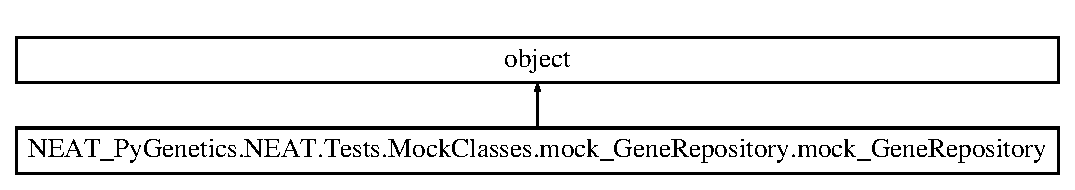
\includegraphics[height=2.000000cm]{class_n_e_a_t___py_genetics_1_1_n_e_a_t_1_1_tests_1_1_mock_classes_1_1mock___gene_repository_1_1mock___gene_repository}
\end{center}
\end{figure}
\subsection*{Public Member Functions}
\begin{DoxyCompactItemize}
\item 
def {\bfseries get\+\_\+gene\+\_\+id\+\_\+for\+\_\+endpoints} (self, head\+\_\+node\+\_\+id, tail\+\_\+node\+\_\+id)\hypertarget{class_n_e_a_t___py_genetics_1_1_n_e_a_t_1_1_tests_1_1_mock_classes_1_1mock___gene_repository_1_1mock___gene_repository_a7b5eef06e8d2486c49acb86b74f43316}{}\label{class_n_e_a_t___py_genetics_1_1_n_e_a_t_1_1_tests_1_1_mock_classes_1_1mock___gene_repository_1_1mock___gene_repository_a7b5eef06e8d2486c49acb86b74f43316}

\item 
def {\bfseries find\+\_\+connecting\+\_\+node} (self, head\+\_\+node\+\_\+id, tail\+\_\+node\+\_\+id)\hypertarget{class_n_e_a_t___py_genetics_1_1_n_e_a_t_1_1_tests_1_1_mock_classes_1_1mock___gene_repository_1_1mock___gene_repository_af8237f68a2528e68c6984225bc9a116f}{}\label{class_n_e_a_t___py_genetics_1_1_n_e_a_t_1_1_tests_1_1_mock_classes_1_1mock___gene_repository_1_1mock___gene_repository_af8237f68a2528e68c6984225bc9a116f}

\item 
def {\bfseries get\+\_\+next\+\_\+node\+\_\+id} (self)\hypertarget{class_n_e_a_t___py_genetics_1_1_n_e_a_t_1_1_tests_1_1_mock_classes_1_1mock___gene_repository_1_1mock___gene_repository_a496072cac2263f4b7213ba45f4458883}{}\label{class_n_e_a_t___py_genetics_1_1_n_e_a_t_1_1_tests_1_1_mock_classes_1_1mock___gene_repository_1_1mock___gene_repository_a496072cac2263f4b7213ba45f4458883}

\end{DoxyCompactItemize}


\subsection{Detailed Description}


Definition at line 2 of file mock\+\_\+\+Gene\+Repository.\+py.



The documentation for this class was generated from the following file\+:\begin{DoxyCompactItemize}
\item 
N\+E\+A\+T/\+Tests/\+Mock\+Classes/mock\+\_\+\+Gene\+Repository.\+py\end{DoxyCompactItemize}

\hypertarget{class_n_e_a_t___py_genetics_1_1_n_e_a_t_1_1_tests_1_1_mock_classes_1_1mock___genome_repository_1_1mock___genome_repository}{}\section{N\+E\+A\+T\+\_\+\+Py\+Genetics.\+N\+E\+A\+T.\+Tests.\+Mock\+Classes.\+mock\+\_\+\+Genome\+Repository.\+mock\+\_\+\+Genome\+Repository Class Reference}
\label{class_n_e_a_t___py_genetics_1_1_n_e_a_t_1_1_tests_1_1_mock_classes_1_1mock___genome_repository_1_1mock___genome_repository}\index{N\+E\+A\+T\+\_\+\+Py\+Genetics.\+N\+E\+A\+T.\+Tests.\+Mock\+Classes.\+mock\+\_\+\+Genome\+Repository.\+mock\+\_\+\+Genome\+Repository@{N\+E\+A\+T\+\_\+\+Py\+Genetics.\+N\+E\+A\+T.\+Tests.\+Mock\+Classes.\+mock\+\_\+\+Genome\+Repository.\+mock\+\_\+\+Genome\+Repository}}
Inheritance diagram for N\+E\+A\+T\+\_\+\+Py\+Genetics.\+N\+E\+A\+T.\+Tests.\+Mock\+Classes.\+mock\+\_\+\+Genome\+Repository.\+mock\+\_\+\+Genome\+Repository\+:\begin{figure}[H]
\begin{center}
\leavevmode
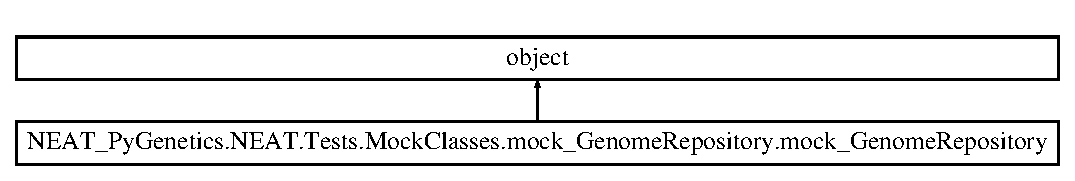
\includegraphics[height=1.982301cm]{class_n_e_a_t___py_genetics_1_1_n_e_a_t_1_1_tests_1_1_mock_classes_1_1mock___genome_repository_1_1mock___genome_repository}
\end{center}
\end{figure}
\subsection*{Public Member Functions}
\begin{DoxyCompactItemize}
\item 
def {\bfseries \+\_\+\+\_\+init\+\_\+\+\_\+} (self)\hypertarget{class_n_e_a_t___py_genetics_1_1_n_e_a_t_1_1_tests_1_1_mock_classes_1_1mock___genome_repository_1_1mock___genome_repository_a1b6913e42019740f0dd683eef2bf8f32}{}\label{class_n_e_a_t___py_genetics_1_1_n_e_a_t_1_1_tests_1_1_mock_classes_1_1mock___genome_repository_1_1mock___genome_repository_a1b6913e42019740f0dd683eef2bf8f32}

\item 
def {\bfseries get\+\_\+current\+\_\+population} (self)\hypertarget{class_n_e_a_t___py_genetics_1_1_n_e_a_t_1_1_tests_1_1_mock_classes_1_1mock___genome_repository_1_1mock___genome_repository_ad5413865b1a0a82964e0046d59406383}{}\label{class_n_e_a_t___py_genetics_1_1_n_e_a_t_1_1_tests_1_1_mock_classes_1_1mock___genome_repository_1_1mock___genome_repository_ad5413865b1a0a82964e0046d59406383}

\item 
def {\bfseries update\+\_\+cluster\+\_\+for\+\_\+genome}\hypertarget{class_n_e_a_t___py_genetics_1_1_n_e_a_t_1_1_tests_1_1_mock_classes_1_1mock___genome_repository_1_1mock___genome_repository_a3d3a5d43fa4285aa6282557fef12f471}{}\label{class_n_e_a_t___py_genetics_1_1_n_e_a_t_1_1_tests_1_1_mock_classes_1_1mock___genome_repository_1_1mock___genome_repository_a3d3a5d43fa4285aa6282557fef12f471}

\item 
def {\bfseries get\+\_\+genome\+\_\+by\+\_\+id}\hypertarget{class_n_e_a_t___py_genetics_1_1_n_e_a_t_1_1_tests_1_1_mock_classes_1_1mock___genome_repository_1_1mock___genome_repository_aab8cb8b23202bf0a41e3dcbf42c096b0}{}\label{class_n_e_a_t___py_genetics_1_1_n_e_a_t_1_1_tests_1_1_mock_classes_1_1mock___genome_repository_1_1mock___genome_repository_aab8cb8b23202bf0a41e3dcbf42c096b0}

\item 
def {\bfseries get\+\_\+genomes\+\_\+in\+\_\+cluster}\hypertarget{class_n_e_a_t___py_genetics_1_1_n_e_a_t_1_1_tests_1_1_mock_classes_1_1mock___genome_repository_1_1mock___genome_repository_a5abad1601614b0c128b4ab64e41ecba8}{}\label{class_n_e_a_t___py_genetics_1_1_n_e_a_t_1_1_tests_1_1_mock_classes_1_1mock___genome_repository_1_1mock___genome_repository_a5abad1601614b0c128b4ab64e41ecba8}

\end{DoxyCompactItemize}
\subsection*{Public Attributes}
\begin{DoxyCompactItemize}
\item 
{\bfseries mock\+\_\+population}\hypertarget{class_n_e_a_t___py_genetics_1_1_n_e_a_t_1_1_tests_1_1_mock_classes_1_1mock___genome_repository_1_1mock___genome_repository_abb2dfb4fa59c22b09dede3bcbd27ca4b}{}\label{class_n_e_a_t___py_genetics_1_1_n_e_a_t_1_1_tests_1_1_mock_classes_1_1mock___genome_repository_1_1mock___genome_repository_abb2dfb4fa59c22b09dede3bcbd27ca4b}

\end{DoxyCompactItemize}


\subsection{Detailed Description}


Definition at line 5 of file mock\+\_\+\+Genome\+Repository.\+py.



The documentation for this class was generated from the following file\+:\begin{DoxyCompactItemize}
\item 
N\+E\+A\+T/\+Tests/\+Mock\+Classes/mock\+\_\+\+Genome\+Repository.\+py\end{DoxyCompactItemize}

\hypertarget{class_n_e_a_t___py_genetics_1_1_n_e_a_t_1_1_generator_1_1_mutator_1_1_mutator}{}\section{N\+E\+A\+T\+\_\+\+Py\+Genetics.\+N\+E\+A\+T.\+Generator.\+Mutator.\+Mutator Class Reference}
\label{class_n_e_a_t___py_genetics_1_1_n_e_a_t_1_1_generator_1_1_mutator_1_1_mutator}\index{N\+E\+A\+T\+\_\+\+Py\+Genetics.\+N\+E\+A\+T.\+Generator.\+Mutator.\+Mutator@{N\+E\+A\+T\+\_\+\+Py\+Genetics.\+N\+E\+A\+T.\+Generator.\+Mutator.\+Mutator}}
Inheritance diagram for N\+E\+A\+T\+\_\+\+Py\+Genetics.\+N\+E\+A\+T.\+Generator.\+Mutator.\+Mutator\+:\begin{figure}[H]
\begin{center}
\leavevmode
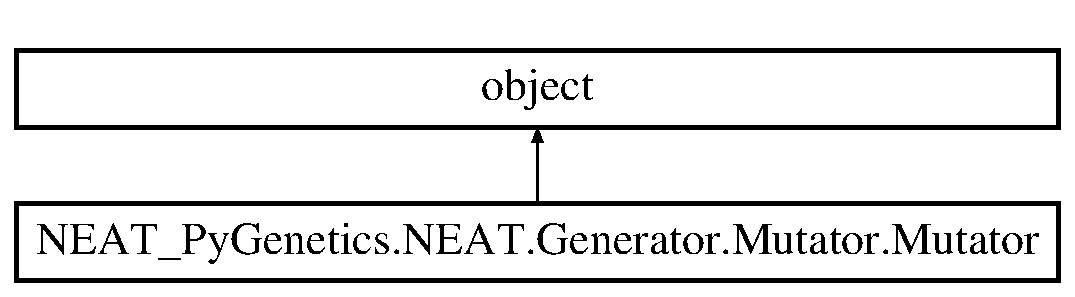
\includegraphics[height=2.000000cm]{class_n_e_a_t___py_genetics_1_1_n_e_a_t_1_1_generator_1_1_mutator_1_1_mutator}
\end{center}
\end{figure}
\subsection*{Public Member Functions}
\begin{DoxyCompactItemize}
\item 
def {\bfseries \+\_\+\+\_\+init\+\_\+\+\_\+} (self, gene\+\_\+repository, mutation\+\_\+parameters)\hypertarget{class_n_e_a_t___py_genetics_1_1_n_e_a_t_1_1_generator_1_1_mutator_1_1_mutator_aef75e9ceb50c5d6df86ab49132a1fe84}{}\label{class_n_e_a_t___py_genetics_1_1_n_e_a_t_1_1_generator_1_1_mutator_1_1_mutator_aef75e9ceb50c5d6df86ab49132a1fe84}

\item 
def {\bfseries mutate\+\_\+genome} (self, genome)\hypertarget{class_n_e_a_t___py_genetics_1_1_n_e_a_t_1_1_generator_1_1_mutator_1_1_mutator_aa805f3b8374dcf45ab4406f48bf145d5}{}\label{class_n_e_a_t___py_genetics_1_1_n_e_a_t_1_1_generator_1_1_mutator_1_1_mutator_aa805f3b8374dcf45ab4406f48bf145d5}

\item 
def {\bfseries mutate\+\_\+add\+\_\+edge}\hypertarget{class_n_e_a_t___py_genetics_1_1_n_e_a_t_1_1_generator_1_1_mutator_1_1_mutator_aaee3498341c20339761db1301af7f341}{}\label{class_n_e_a_t___py_genetics_1_1_n_e_a_t_1_1_generator_1_1_mutator_1_1_mutator_aaee3498341c20339761db1301af7f341}

\item 
def {\bfseries mutate\+\_\+add\+\_\+node}\hypertarget{class_n_e_a_t___py_genetics_1_1_n_e_a_t_1_1_generator_1_1_mutator_1_1_mutator_afeabd93fc71a47574e11dd8ac86b1cc2}{}\label{class_n_e_a_t___py_genetics_1_1_n_e_a_t_1_1_generator_1_1_mutator_1_1_mutator_afeabd93fc71a47574e11dd8ac86b1cc2}

\item 
def {\bfseries mutate\+\_\+perturb\+\_\+weights}\hypertarget{class_n_e_a_t___py_genetics_1_1_n_e_a_t_1_1_generator_1_1_mutator_1_1_mutator_aecb97c840811304711e07fe159b0c4bd}{}\label{class_n_e_a_t___py_genetics_1_1_n_e_a_t_1_1_generator_1_1_mutator_1_1_mutator_aecb97c840811304711e07fe159b0c4bd}

\end{DoxyCompactItemize}
\subsection*{Static Public Member Functions}
\begin{DoxyCompactItemize}
\item 
def {\bfseries perturb\+\_\+weight}\hypertarget{class_n_e_a_t___py_genetics_1_1_n_e_a_t_1_1_generator_1_1_mutator_1_1_mutator_ae8e05c9ff54df03a83a0809a7ba1f00a}{}\label{class_n_e_a_t___py_genetics_1_1_n_e_a_t_1_1_generator_1_1_mutator_1_1_mutator_ae8e05c9ff54df03a83a0809a7ba1f00a}

\end{DoxyCompactItemize}
\subsection*{Public Attributes}
\begin{DoxyCompactItemize}
\item 
{\bfseries gene\+\_\+repository}\hypertarget{class_n_e_a_t___py_genetics_1_1_n_e_a_t_1_1_generator_1_1_mutator_1_1_mutator_afa98da8eee10b2a4e9c653238dbbbe2c}{}\label{class_n_e_a_t___py_genetics_1_1_n_e_a_t_1_1_generator_1_1_mutator_1_1_mutator_afa98da8eee10b2a4e9c653238dbbbe2c}

\item 
{\bfseries mutation\+\_\+parameters}\hypertarget{class_n_e_a_t___py_genetics_1_1_n_e_a_t_1_1_generator_1_1_mutator_1_1_mutator_a3339255b05437da752358f068835bc26}{}\label{class_n_e_a_t___py_genetics_1_1_n_e_a_t_1_1_generator_1_1_mutator_1_1_mutator_a3339255b05437da752358f068835bc26}

\end{DoxyCompactItemize}
\subsection*{Static Public Attributes}
\begin{DoxyCompactItemize}
\item 
{\bfseries starting\+\_\+vertex}\hypertarget{class_n_e_a_t___py_genetics_1_1_n_e_a_t_1_1_generator_1_1_mutator_1_1_mutator_a74faa3a8d9acd9c1c0a68e145441fc5b}{}\label{class_n_e_a_t___py_genetics_1_1_n_e_a_t_1_1_generator_1_1_mutator_1_1_mutator_a74faa3a8d9acd9c1c0a68e145441fc5b}

\item 
{\bfseries possible\+\_\+endpoints}\hypertarget{class_n_e_a_t___py_genetics_1_1_n_e_a_t_1_1_generator_1_1_mutator_1_1_mutator_add17af09898bf2a4203fed77bc404161}{}\label{class_n_e_a_t___py_genetics_1_1_n_e_a_t_1_1_generator_1_1_mutator_1_1_mutator_add17af09898bf2a4203fed77bc404161}

\item 
{\bfseries endpoint}\hypertarget{class_n_e_a_t___py_genetics_1_1_n_e_a_t_1_1_generator_1_1_mutator_1_1_mutator_a7f7f636e283125c144a7781a6ac5afaa}{}\label{class_n_e_a_t___py_genetics_1_1_n_e_a_t_1_1_generator_1_1_mutator_1_1_mutator_a7f7f636e283125c144a7781a6ac5afaa}

\item 
{\bfseries gene\+\_\+id}\hypertarget{class_n_e_a_t___py_genetics_1_1_n_e_a_t_1_1_generator_1_1_mutator_1_1_mutator_a6479cbdd1acaed28cbdbdbc6d663ec89}{}\label{class_n_e_a_t___py_genetics_1_1_n_e_a_t_1_1_generator_1_1_mutator_1_1_mutator_a6479cbdd1acaed28cbdbdbc6d663ec89}

\item 
{\bfseries gene\+\_\+weight}\hypertarget{class_n_e_a_t___py_genetics_1_1_n_e_a_t_1_1_generator_1_1_mutator_1_1_mutator_a85333a494bf1858ec78e1a304c5c25ec}{}\label{class_n_e_a_t___py_genetics_1_1_n_e_a_t_1_1_generator_1_1_mutator_1_1_mutator_a85333a494bf1858ec78e1a304c5c25ec}

\item 
{\bfseries gene\+\_\+enabled}\hypertarget{class_n_e_a_t___py_genetics_1_1_n_e_a_t_1_1_generator_1_1_mutator_1_1_mutator_a231e7983bed77578ecaa3d9b1d13e037}{}\label{class_n_e_a_t___py_genetics_1_1_n_e_a_t_1_1_generator_1_1_mutator_1_1_mutator_a231e7983bed77578ecaa3d9b1d13e037}

\item 
{\bfseries new\+\_\+genome}\hypertarget{class_n_e_a_t___py_genetics_1_1_n_e_a_t_1_1_generator_1_1_mutator_1_1_mutator_a738d393eb3669111cf0fda1485019ca3}{}\label{class_n_e_a_t___py_genetics_1_1_n_e_a_t_1_1_generator_1_1_mutator_1_1_mutator_a738d393eb3669111cf0fda1485019ca3}

\item 
{\bfseries old\+\_\+gene\+\_\+id}\hypertarget{class_n_e_a_t___py_genetics_1_1_n_e_a_t_1_1_generator_1_1_mutator_1_1_mutator_a65fc450affae2ea20311a30dc4fb69af}{}\label{class_n_e_a_t___py_genetics_1_1_n_e_a_t_1_1_generator_1_1_mutator_1_1_mutator_a65fc450affae2ea20311a30dc4fb69af}

\item 
{\bfseries old\+\_\+gene}\hypertarget{class_n_e_a_t___py_genetics_1_1_n_e_a_t_1_1_generator_1_1_mutator_1_1_mutator_a0dfab1f6afdafcbcb3f907471b66d588}{}\label{class_n_e_a_t___py_genetics_1_1_n_e_a_t_1_1_generator_1_1_mutator_1_1_mutator_a0dfab1f6afdafcbcb3f907471b66d588}

\item 
{\bfseries connecting\+\_\+nodes}\hypertarget{class_n_e_a_t___py_genetics_1_1_n_e_a_t_1_1_generator_1_1_mutator_1_1_mutator_a2b1d1d4ca57366264f0e1648c575023f}{}\label{class_n_e_a_t___py_genetics_1_1_n_e_a_t_1_1_generator_1_1_mutator_1_1_mutator_a2b1d1d4ca57366264f0e1648c575023f}

\item 
{\bfseries connecting\+\_\+node}\hypertarget{class_n_e_a_t___py_genetics_1_1_n_e_a_t_1_1_generator_1_1_mutator_1_1_mutator_aeaff4debf91f61a735965c3533ae1e6c}{}\label{class_n_e_a_t___py_genetics_1_1_n_e_a_t_1_1_generator_1_1_mutator_1_1_mutator_aeaff4debf91f61a735965c3533ae1e6c}

\item 
{\bfseries new\+\_\+gene\+\_\+one\+\_\+id}\hypertarget{class_n_e_a_t___py_genetics_1_1_n_e_a_t_1_1_generator_1_1_mutator_1_1_mutator_a346f32875edc5cb74b3d3555eaea80f9}{}\label{class_n_e_a_t___py_genetics_1_1_n_e_a_t_1_1_generator_1_1_mutator_1_1_mutator_a346f32875edc5cb74b3d3555eaea80f9}

\item 
{\bfseries new\+\_\+gene\+\_\+one\+\_\+weight}\hypertarget{class_n_e_a_t___py_genetics_1_1_n_e_a_t_1_1_generator_1_1_mutator_1_1_mutator_a77e03377943c33be52a1da66028c9386}{}\label{class_n_e_a_t___py_genetics_1_1_n_e_a_t_1_1_generator_1_1_mutator_1_1_mutator_a77e03377943c33be52a1da66028c9386}

\item 
{\bfseries new\+\_\+gene\+\_\+one}\hypertarget{class_n_e_a_t___py_genetics_1_1_n_e_a_t_1_1_generator_1_1_mutator_1_1_mutator_a18e697e12c153b9679c214f9737f5f9c}{}\label{class_n_e_a_t___py_genetics_1_1_n_e_a_t_1_1_generator_1_1_mutator_1_1_mutator_a18e697e12c153b9679c214f9737f5f9c}

\item 
{\bfseries new\+\_\+gene\+\_\+two\+\_\+id}\hypertarget{class_n_e_a_t___py_genetics_1_1_n_e_a_t_1_1_generator_1_1_mutator_1_1_mutator_a3fcf4df1bdecbc52e92ae8f63d38d473}{}\label{class_n_e_a_t___py_genetics_1_1_n_e_a_t_1_1_generator_1_1_mutator_1_1_mutator_a3fcf4df1bdecbc52e92ae8f63d38d473}

\item 
{\bfseries new\+\_\+gene\+\_\+two}\hypertarget{class_n_e_a_t___py_genetics_1_1_n_e_a_t_1_1_generator_1_1_mutator_1_1_mutator_a3380ad2d05e8eace2063d8f1791274e0}{}\label{class_n_e_a_t___py_genetics_1_1_n_e_a_t_1_1_generator_1_1_mutator_1_1_mutator_a3380ad2d05e8eace2063d8f1791274e0}

\item 
{\bfseries new\+\_\+weight}\hypertarget{class_n_e_a_t___py_genetics_1_1_n_e_a_t_1_1_generator_1_1_mutator_1_1_mutator_a21e659d59a5f4ac929795dc4f5036f44}{}\label{class_n_e_a_t___py_genetics_1_1_n_e_a_t_1_1_generator_1_1_mutator_1_1_mutator_a21e659d59a5f4ac929795dc4f5036f44}

\end{DoxyCompactItemize}


\subsection{Detailed Description}


Definition at line 11 of file Mutator.\+py.



The documentation for this class was generated from the following file\+:\begin{DoxyCompactItemize}
\item 
N\+E\+A\+T/\+Generator/Mutator.\+py\end{DoxyCompactItemize}

\hypertarget{class_n_e_a_t___py_genetics_1_1_n_e_a_t_1_1_networking_1_1_client_1_1_n_e_a_t_client_1_1_n_e_a_t_client}{}\section{N\+E\+A\+T\+\_\+\+Py\+Genetics.\+N\+E\+A\+T.\+Networking.\+Client.\+N\+E\+A\+T\+Client.\+N\+E\+A\+T\+Client Class Reference}
\label{class_n_e_a_t___py_genetics_1_1_n_e_a_t_1_1_networking_1_1_client_1_1_n_e_a_t_client_1_1_n_e_a_t_client}\index{N\+E\+A\+T\+\_\+\+Py\+Genetics.\+N\+E\+A\+T.\+Networking.\+Client.\+N\+E\+A\+T\+Client.\+N\+E\+A\+T\+Client@{N\+E\+A\+T\+\_\+\+Py\+Genetics.\+N\+E\+A\+T.\+Networking.\+Client.\+N\+E\+A\+T\+Client.\+N\+E\+A\+T\+Client}}
Inheritance diagram for N\+E\+A\+T\+\_\+\+Py\+Genetics.\+N\+E\+A\+T.\+Networking.\+Client.\+N\+E\+A\+T\+Client.\+N\+E\+A\+T\+Client\+:\begin{figure}[H]
\begin{center}
\leavevmode
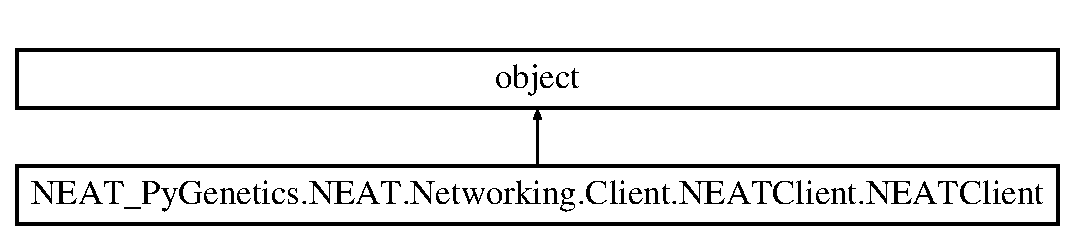
\includegraphics[height=2.000000cm]{class_n_e_a_t___py_genetics_1_1_n_e_a_t_1_1_networking_1_1_client_1_1_n_e_a_t_client_1_1_n_e_a_t_client}
\end{center}
\end{figure}
\subsection*{Public Member Functions}
\begin{DoxyCompactItemize}
\item 
def {\bfseries \+\_\+\+\_\+init\+\_\+\+\_\+} (self, server\+\_\+address, server\+\_\+port)\hypertarget{class_n_e_a_t___py_genetics_1_1_n_e_a_t_1_1_networking_1_1_client_1_1_n_e_a_t_client_1_1_n_e_a_t_client_a9e84283e9dab07424cbbef8d966fd74b}{}\label{class_n_e_a_t___py_genetics_1_1_n_e_a_t_1_1_networking_1_1_client_1_1_n_e_a_t_client_1_1_n_e_a_t_client_a9e84283e9dab07424cbbef8d966fd74b}

\item 
def {\bfseries run\+\_\+command} (self, command)\hypertarget{class_n_e_a_t___py_genetics_1_1_n_e_a_t_1_1_networking_1_1_client_1_1_n_e_a_t_client_1_1_n_e_a_t_client_a58156abc06c16b0f2399219655c7321c}{}\label{class_n_e_a_t___py_genetics_1_1_n_e_a_t_1_1_networking_1_1_client_1_1_n_e_a_t_client_1_1_n_e_a_t_client_a58156abc06c16b0f2399219655c7321c}

\end{DoxyCompactItemize}


\subsection{Detailed Description}


Definition at line 5 of file N\+E\+A\+T\+Client.\+py.



The documentation for this class was generated from the following file\+:\begin{DoxyCompactItemize}
\item 
N\+E\+A\+T/\+Networking/\+Client/N\+E\+A\+T\+Client.\+py\end{DoxyCompactItemize}

\hypertarget{class_n_e_a_t___py_genetics_1_1_n_e_a_t_1_1_config_1_1_n_e_a_t_config_1_1_n_e_a_t_config}{}\section{N\+E\+A\+T\+\_\+\+Py\+Genetics.\+N\+E\+A\+T.\+Config.\+N\+E\+A\+T\+Config.\+N\+E\+A\+T\+Config Class Reference}
\label{class_n_e_a_t___py_genetics_1_1_n_e_a_t_1_1_config_1_1_n_e_a_t_config_1_1_n_e_a_t_config}\index{N\+E\+A\+T\+\_\+\+Py\+Genetics.\+N\+E\+A\+T.\+Config.\+N\+E\+A\+T\+Config.\+N\+E\+A\+T\+Config@{N\+E\+A\+T\+\_\+\+Py\+Genetics.\+N\+E\+A\+T.\+Config.\+N\+E\+A\+T\+Config.\+N\+E\+A\+T\+Config}}
Inheritance diagram for N\+E\+A\+T\+\_\+\+Py\+Genetics.\+N\+E\+A\+T.\+Config.\+N\+E\+A\+T\+Config.\+N\+E\+A\+T\+Config\+:\begin{figure}[H]
\begin{center}
\leavevmode
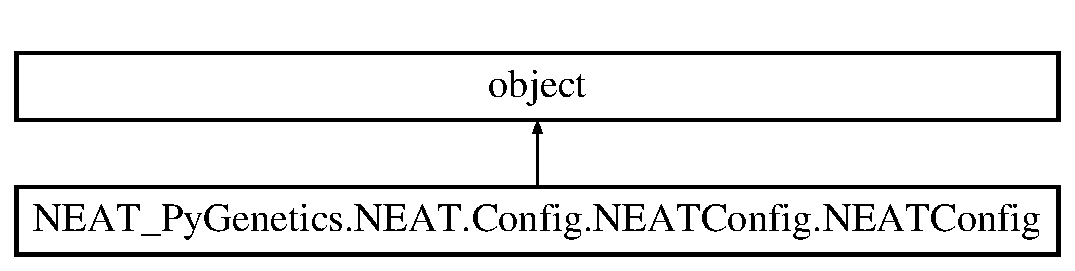
\includegraphics[height=2.000000cm]{class_n_e_a_t___py_genetics_1_1_n_e_a_t_1_1_config_1_1_n_e_a_t_config_1_1_n_e_a_t_config}
\end{center}
\end{figure}
\subsection*{Public Member Functions}
\begin{DoxyCompactItemize}
\item 
def {\bfseries \+\_\+\+\_\+init\+\_\+\+\_\+} (self, config\+\_\+path=None)\hypertarget{class_n_e_a_t___py_genetics_1_1_n_e_a_t_1_1_config_1_1_n_e_a_t_config_1_1_n_e_a_t_config_a88504e0a5c56f166a3ee5898ae3e0dea}{}\label{class_n_e_a_t___py_genetics_1_1_n_e_a_t_1_1_config_1_1_n_e_a_t_config_1_1_n_e_a_t_config_a88504e0a5c56f166a3ee5898ae3e0dea}

\item 
def \hyperlink{class_n_e_a_t___py_genetics_1_1_n_e_a_t_1_1_config_1_1_n_e_a_t_config_1_1_n_e_a_t_config_aa6843226e3a017a384c8244f4e62e0f5}{load\+\_\+config} (self)
\item 
def \hyperlink{class_n_e_a_t___py_genetics_1_1_n_e_a_t_1_1_config_1_1_n_e_a_t_config_1_1_n_e_a_t_config_a2669153b4f4160d33477fc89d16dd716}{load\+\_\+defaults} (self)
\end{DoxyCompactItemize}
\subsection*{Public Attributes}
\begin{DoxyCompactItemize}
\item 
{\bfseries parameters}\hypertarget{class_n_e_a_t___py_genetics_1_1_n_e_a_t_1_1_config_1_1_n_e_a_t_config_1_1_n_e_a_t_config_a04ae4f640ee3d8a9dadbbe0a293bb3d6}{}\label{class_n_e_a_t___py_genetics_1_1_n_e_a_t_1_1_config_1_1_n_e_a_t_config_1_1_n_e_a_t_config_a04ae4f640ee3d8a9dadbbe0a293bb3d6}

\item 
{\bfseries config\+\_\+directory}\hypertarget{class_n_e_a_t___py_genetics_1_1_n_e_a_t_1_1_config_1_1_n_e_a_t_config_1_1_n_e_a_t_config_ae3bd7eb4a5b4ad753d5c2de3c70aed06}{}\label{class_n_e_a_t___py_genetics_1_1_n_e_a_t_1_1_config_1_1_n_e_a_t_config_1_1_n_e_a_t_config_ae3bd7eb4a5b4ad753d5c2de3c70aed06}

\item 
{\bfseries working\+\_\+directory}\hypertarget{class_n_e_a_t___py_genetics_1_1_n_e_a_t_1_1_config_1_1_n_e_a_t_config_1_1_n_e_a_t_config_ac88a0f28d412192f52a5cb55935beaa4}{}\label{class_n_e_a_t___py_genetics_1_1_n_e_a_t_1_1_config_1_1_n_e_a_t_config_1_1_n_e_a_t_config_ac88a0f28d412192f52a5cb55935beaa4}

\item 
{\bfseries config\+\_\+categories}\hypertarget{class_n_e_a_t___py_genetics_1_1_n_e_a_t_1_1_config_1_1_n_e_a_t_config_1_1_n_e_a_t_config_a1e2b0edc6558d673c7f7a197d2faa72e}{}\label{class_n_e_a_t___py_genetics_1_1_n_e_a_t_1_1_config_1_1_n_e_a_t_config_1_1_n_e_a_t_config_a1e2b0edc6558d673c7f7a197d2faa72e}

\end{DoxyCompactItemize}


\subsection{Detailed Description}
\begin{DoxyVerb}A huge configuration object which loads it's parameters
from disk, or reverts to default values whenever a
configuration file isn't found or can't be opened.
Config files are in JSON notation.

Configuration files are listed in self.config_categories
and should be present as CATEGORYNAME.conf in the
provided config_path. If no config path is specified, the builtin
config files in NEAT/Config are used.

All config files except one can be loaded from defaults.
The only exception is genomes.conf, the config file specifying
the input and output nodes of the genomes to use, because it
is dependent on the simulation.
\end{DoxyVerb}
 

Definition at line 7 of file N\+E\+A\+T\+Config.\+py.



\subsection{Member Function Documentation}
\index{N\+E\+A\+T\+\_\+\+Py\+Genetics\+::\+N\+E\+A\+T\+::\+Config\+::\+N\+E\+A\+T\+Config\+::\+N\+E\+A\+T\+Config@{N\+E\+A\+T\+\_\+\+Py\+Genetics\+::\+N\+E\+A\+T\+::\+Config\+::\+N\+E\+A\+T\+Config\+::\+N\+E\+A\+T\+Config}!load\+\_\+config@{load\+\_\+config}}
\index{load\+\_\+config@{load\+\_\+config}!N\+E\+A\+T\+\_\+\+Py\+Genetics\+::\+N\+E\+A\+T\+::\+Config\+::\+N\+E\+A\+T\+Config\+::\+N\+E\+A\+T\+Config@{N\+E\+A\+T\+\_\+\+Py\+Genetics\+::\+N\+E\+A\+T\+::\+Config\+::\+N\+E\+A\+T\+Config\+::\+N\+E\+A\+T\+Config}}
\subsubsection[{\texorpdfstring{load\+\_\+config(self)}{load_config(self)}}]{\setlength{\rightskip}{0pt plus 5cm}def N\+E\+A\+T\+\_\+\+Py\+Genetics.\+N\+E\+A\+T.\+Config.\+N\+E\+A\+T\+Config.\+N\+E\+A\+T\+Config.\+load\+\_\+config (
\begin{DoxyParamCaption}
\item[{}]{self}
\end{DoxyParamCaption}
)}\hypertarget{class_n_e_a_t___py_genetics_1_1_n_e_a_t_1_1_config_1_1_n_e_a_t_config_1_1_n_e_a_t_config_aa6843226e3a017a384c8244f4e62e0f5}{}\label{class_n_e_a_t___py_genetics_1_1_n_e_a_t_1_1_config_1_1_n_e_a_t_config_1_1_n_e_a_t_config_aa6843226e3a017a384c8244f4e62e0f5}
\begin{DoxyVerb}Tries to initialize self.parameters with data
from the configuration files. It uses the base file
names from self.config_categories and is agnostic to the number
and names of the existing categories.
Config files need to be in JSON notation.

:return: None
\end{DoxyVerb}
 

Definition at line 50 of file N\+E\+A\+T\+Config.\+py.

\index{N\+E\+A\+T\+\_\+\+Py\+Genetics\+::\+N\+E\+A\+T\+::\+Config\+::\+N\+E\+A\+T\+Config\+::\+N\+E\+A\+T\+Config@{N\+E\+A\+T\+\_\+\+Py\+Genetics\+::\+N\+E\+A\+T\+::\+Config\+::\+N\+E\+A\+T\+Config\+::\+N\+E\+A\+T\+Config}!load\+\_\+defaults@{load\+\_\+defaults}}
\index{load\+\_\+defaults@{load\+\_\+defaults}!N\+E\+A\+T\+\_\+\+Py\+Genetics\+::\+N\+E\+A\+T\+::\+Config\+::\+N\+E\+A\+T\+Config\+::\+N\+E\+A\+T\+Config@{N\+E\+A\+T\+\_\+\+Py\+Genetics\+::\+N\+E\+A\+T\+::\+Config\+::\+N\+E\+A\+T\+Config\+::\+N\+E\+A\+T\+Config}}
\subsubsection[{\texorpdfstring{load\+\_\+defaults(self)}{load_defaults(self)}}]{\setlength{\rightskip}{0pt plus 5cm}def N\+E\+A\+T\+\_\+\+Py\+Genetics.\+N\+E\+A\+T.\+Config.\+N\+E\+A\+T\+Config.\+N\+E\+A\+T\+Config.\+load\+\_\+defaults (
\begin{DoxyParamCaption}
\item[{}]{self}
\end{DoxyParamCaption}
)}\hypertarget{class_n_e_a_t___py_genetics_1_1_n_e_a_t_1_1_config_1_1_n_e_a_t_config_1_1_n_e_a_t_config_a2669153b4f4160d33477fc89d16dd716}{}\label{class_n_e_a_t___py_genetics_1_1_n_e_a_t_1_1_config_1_1_n_e_a_t_config_1_1_n_e_a_t_config_a2669153b4f4160d33477fc89d16dd716}
\begin{DoxyVerb}This method is called by __init__ after the config
files are loaded. It's job is to test whether the
config files were loaded by self.load_config() and provide
the appropriate default values (or crash if there are no defaults)
for the missing config parameters.

Because this error-handling method cannot rely on file I/O,
the defaults are hard-coded.

:return: None
\end{DoxyVerb}
 

Definition at line 77 of file N\+E\+A\+T\+Config.\+py.



The documentation for this class was generated from the following file\+:\begin{DoxyCompactItemize}
\item 
N\+E\+A\+T/\+Config/N\+E\+A\+T\+Config.\+py\end{DoxyCompactItemize}

\hypertarget{class_n_e_a_t___py_genetics_1_1_n_e_a_t_1_1_networking_1_1_server_1_1_n_e_a_t_server_1_1_n_e_a_t_server}{}\section{N\+E\+A\+T\+\_\+\+Py\+Genetics.\+N\+E\+A\+T.\+Networking.\+Server.\+N\+E\+A\+T\+Server.\+N\+E\+A\+T\+Server Class Reference}
\label{class_n_e_a_t___py_genetics_1_1_n_e_a_t_1_1_networking_1_1_server_1_1_n_e_a_t_server_1_1_n_e_a_t_server}\index{N\+E\+A\+T\+\_\+\+Py\+Genetics.\+N\+E\+A\+T.\+Networking.\+Server.\+N\+E\+A\+T\+Server.\+N\+E\+A\+T\+Server@{N\+E\+A\+T\+\_\+\+Py\+Genetics.\+N\+E\+A\+T.\+Networking.\+Server.\+N\+E\+A\+T\+Server.\+N\+E\+A\+T\+Server}}
Inheritance diagram for N\+E\+A\+T\+\_\+\+Py\+Genetics.\+N\+E\+A\+T.\+Networking.\+Server.\+N\+E\+A\+T\+Server.\+N\+E\+A\+T\+Server\+:\begin{figure}[H]
\begin{center}
\leavevmode
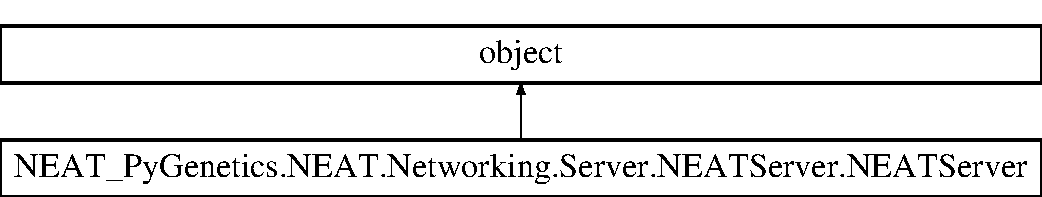
\includegraphics[height=2.000000cm]{class_n_e_a_t___py_genetics_1_1_n_e_a_t_1_1_networking_1_1_server_1_1_n_e_a_t_server_1_1_n_e_a_t_server}
\end{center}
\end{figure}
\subsection*{Public Member Functions}
\begin{DoxyCompactItemize}
\item 
def {\bfseries \+\_\+\+\_\+init\+\_\+\+\_\+} (self)\hypertarget{class_n_e_a_t___py_genetics_1_1_n_e_a_t_1_1_networking_1_1_server_1_1_n_e_a_t_server_1_1_n_e_a_t_server_a45eb9c4003d9e0f4ae9c0e239423ddad}{}\label{class_n_e_a_t___py_genetics_1_1_n_e_a_t_1_1_networking_1_1_server_1_1_n_e_a_t_server_1_1_n_e_a_t_server_a45eb9c4003d9e0f4ae9c0e239423ddad}

\item 
def {\bfseries respond}\hypertarget{class_n_e_a_t___py_genetics_1_1_n_e_a_t_1_1_networking_1_1_server_1_1_n_e_a_t_server_1_1_n_e_a_t_server_a44ffcc6f56d71844827bd402bf4f0e63}{}\label{class_n_e_a_t___py_genetics_1_1_n_e_a_t_1_1_networking_1_1_server_1_1_n_e_a_t_server_1_1_n_e_a_t_server_a44ffcc6f56d71844827bd402bf4f0e63}

\item 
def {\bfseries fetch}\hypertarget{class_n_e_a_t___py_genetics_1_1_n_e_a_t_1_1_networking_1_1_server_1_1_n_e_a_t_server_1_1_n_e_a_t_server_adf4c43680aa89998cf65bc6499f778a8}{}\label{class_n_e_a_t___py_genetics_1_1_n_e_a_t_1_1_networking_1_1_server_1_1_n_e_a_t_server_1_1_n_e_a_t_server_adf4c43680aa89998cf65bc6499f778a8}

\end{DoxyCompactItemize}
\subsection*{Static Public Attributes}
\begin{DoxyCompactItemize}
\item 
{\bfseries time\+\_\+passed}\hypertarget{class_n_e_a_t___py_genetics_1_1_n_e_a_t_1_1_networking_1_1_server_1_1_n_e_a_t_server_1_1_n_e_a_t_server_acbbd8416ba0d7139131ff0e553b20c3d}{}\label{class_n_e_a_t___py_genetics_1_1_n_e_a_t_1_1_networking_1_1_server_1_1_n_e_a_t_server_1_1_n_e_a_t_server_acbbd8416ba0d7139131ff0e553b20c3d}

\item 
{\bfseries starting\+\_\+time}\hypertarget{class_n_e_a_t___py_genetics_1_1_n_e_a_t_1_1_networking_1_1_server_1_1_n_e_a_t_server_1_1_n_e_a_t_server_abba58b32d9919608f5502e001dbd62dd}{}\label{class_n_e_a_t___py_genetics_1_1_n_e_a_t_1_1_networking_1_1_server_1_1_n_e_a_t_server_1_1_n_e_a_t_server_abba58b32d9919608f5502e001dbd62dd}

\end{DoxyCompactItemize}


\subsection{Detailed Description}
\begin{DoxyVerb}A message queue server that handles sending and receiving
of command objects via the QueueWorker and JSONSocket classes.
\end{DoxyVerb}
 

Definition at line 109 of file N\+E\+A\+T\+Server.\+py.



The documentation for this class was generated from the following file\+:\begin{DoxyCompactItemize}
\item 
N\+E\+A\+T/\+Networking/\+Server/N\+E\+A\+T\+Server.\+py\end{DoxyCompactItemize}

\hypertarget{class_n_e_a_t___py_genetics_1_1_n_e_a_t_1_1_error_handling_1_1_exceptions_1_1_network_protocol_e188125698c575255a18f4dd8d98568df}{}\section{N\+E\+A\+T\+\_\+\+Py\+Genetics.\+N\+E\+A\+T.\+Error\+Handling.\+Exceptions.\+Network\+Protocol\+Exception.\+Network\+Protocol\+Exception Class Reference}
\label{class_n_e_a_t___py_genetics_1_1_n_e_a_t_1_1_error_handling_1_1_exceptions_1_1_network_protocol_e188125698c575255a18f4dd8d98568df}\index{N\+E\+A\+T\+\_\+\+Py\+Genetics.\+N\+E\+A\+T.\+Error\+Handling.\+Exceptions.\+Network\+Protocol\+Exception.\+Network\+Protocol\+Exception@{N\+E\+A\+T\+\_\+\+Py\+Genetics.\+N\+E\+A\+T.\+Error\+Handling.\+Exceptions.\+Network\+Protocol\+Exception.\+Network\+Protocol\+Exception}}
Inheritance diagram for N\+E\+A\+T\+\_\+\+Py\+Genetics.\+N\+E\+A\+T.\+Error\+Handling.\+Exceptions.\+Network\+Protocol\+Exception.\+Network\+Protocol\+Exception\+:\begin{figure}[H]
\begin{center}
\leavevmode
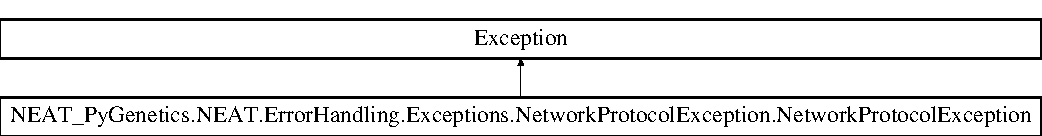
\includegraphics[height=1.824104cm]{class_n_e_a_t___py_genetics_1_1_n_e_a_t_1_1_error_handling_1_1_exceptions_1_1_network_protocol_e188125698c575255a18f4dd8d98568df}
\end{center}
\end{figure}
\subsection*{Public Member Functions}
\begin{DoxyCompactItemize}
\item 
def {\bfseries \+\_\+\+\_\+init\+\_\+\+\_\+} (self, message, errors=None)\hypertarget{class_n_e_a_t___py_genetics_1_1_n_e_a_t_1_1_error_handling_1_1_exceptions_1_1_network_protocol_e188125698c575255a18f4dd8d98568df_a9d12de9b98da65c1a683fe038e066e49}{}\label{class_n_e_a_t___py_genetics_1_1_n_e_a_t_1_1_error_handling_1_1_exceptions_1_1_network_protocol_e188125698c575255a18f4dd8d98568df_a9d12de9b98da65c1a683fe038e066e49}

\end{DoxyCompactItemize}


\subsection{Detailed Description}


Definition at line 1 of file Network\+Protocol\+Exception.\+py.



The documentation for this class was generated from the following file\+:\begin{DoxyCompactItemize}
\item 
N\+E\+A\+T/\+Error\+Handling/\+Exceptions/Network\+Protocol\+Exception.\+py\end{DoxyCompactItemize}

\hypertarget{class_n_e_a_t___py_genetics_1_1_n_e_a_t_1_1_error_handling_1_1_exceptions_1_1_network_timeout_ex09d61843cecde07531bc3d1c6f238646}{}\section{N\+E\+A\+T\+\_\+\+Py\+Genetics.\+N\+E\+A\+T.\+Error\+Handling.\+Exceptions.\+Network\+Timeout\+Exception.\+Network\+Timeout\+Exception Class Reference}
\label{class_n_e_a_t___py_genetics_1_1_n_e_a_t_1_1_error_handling_1_1_exceptions_1_1_network_timeout_ex09d61843cecde07531bc3d1c6f238646}\index{N\+E\+A\+T\+\_\+\+Py\+Genetics.\+N\+E\+A\+T.\+Error\+Handling.\+Exceptions.\+Network\+Timeout\+Exception.\+Network\+Timeout\+Exception@{N\+E\+A\+T\+\_\+\+Py\+Genetics.\+N\+E\+A\+T.\+Error\+Handling.\+Exceptions.\+Network\+Timeout\+Exception.\+Network\+Timeout\+Exception}}
Inheritance diagram for N\+E\+A\+T\+\_\+\+Py\+Genetics.\+N\+E\+A\+T.\+Error\+Handling.\+Exceptions.\+Network\+Timeout\+Exception.\+Network\+Timeout\+Exception\+:\begin{figure}[H]
\begin{center}
\leavevmode
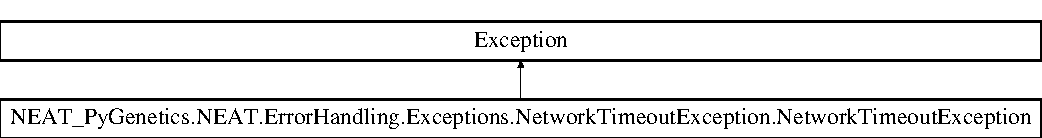
\includegraphics[height=1.848185cm]{class_n_e_a_t___py_genetics_1_1_n_e_a_t_1_1_error_handling_1_1_exceptions_1_1_network_timeout_ex09d61843cecde07531bc3d1c6f238646}
\end{center}
\end{figure}
\subsection*{Public Member Functions}
\begin{DoxyCompactItemize}
\item 
def {\bfseries \+\_\+\+\_\+init\+\_\+\+\_\+} (self, message=\char`\"{}\char`\"{}, errors=None)\hypertarget{class_n_e_a_t___py_genetics_1_1_n_e_a_t_1_1_error_handling_1_1_exceptions_1_1_network_timeout_ex09d61843cecde07531bc3d1c6f238646_ac78b36042b085235de601a15a68ce98a}{}\label{class_n_e_a_t___py_genetics_1_1_n_e_a_t_1_1_error_handling_1_1_exceptions_1_1_network_timeout_ex09d61843cecde07531bc3d1c6f238646_ac78b36042b085235de601a15a68ce98a}

\end{DoxyCompactItemize}


\subsection{Detailed Description}


Definition at line 1 of file Network\+Timeout\+Exception.\+py.



The documentation for this class was generated from the following file\+:\begin{DoxyCompactItemize}
\item 
N\+E\+A\+T/\+Error\+Handling/\+Exceptions/Network\+Timeout\+Exception.\+py\end{DoxyCompactItemize}

\hypertarget{class_n_e_a_t___py_genetics_1_1_n_e_a_t_1_1_genome_structures_1_1_simulation_structure_1_1_simulation_nodes_1_1_node}{}\section{N\+E\+A\+T\+\_\+\+Py\+Genetics.\+N\+E\+A\+T.\+Genome\+Structures.\+Simulation\+Structure.\+Simulation\+Nodes.\+Node Class Reference}
\label{class_n_e_a_t___py_genetics_1_1_n_e_a_t_1_1_genome_structures_1_1_simulation_structure_1_1_simulation_nodes_1_1_node}\index{N\+E\+A\+T\+\_\+\+Py\+Genetics.\+N\+E\+A\+T.\+Genome\+Structures.\+Simulation\+Structure.\+Simulation\+Nodes.\+Node@{N\+E\+A\+T\+\_\+\+Py\+Genetics.\+N\+E\+A\+T.\+Genome\+Structures.\+Simulation\+Structure.\+Simulation\+Nodes.\+Node}}
Inheritance diagram for N\+E\+A\+T\+\_\+\+Py\+Genetics.\+N\+E\+A\+T.\+Genome\+Structures.\+Simulation\+Structure.\+Simulation\+Nodes.\+Node\+:\begin{figure}[H]
\begin{center}
\leavevmode
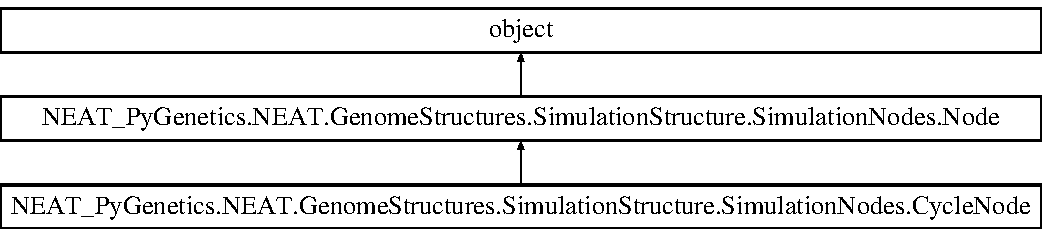
\includegraphics[height=3.000000cm]{class_n_e_a_t___py_genetics_1_1_n_e_a_t_1_1_genome_structures_1_1_simulation_structure_1_1_simulation_nodes_1_1_node}
\end{center}
\end{figure}
\subsection*{Public Member Functions}
\begin{DoxyCompactItemize}
\item 
def {\bfseries \+\_\+\+\_\+init\+\_\+\+\_\+}\hypertarget{class_n_e_a_t___py_genetics_1_1_n_e_a_t_1_1_genome_structures_1_1_simulation_structure_1_1_simulation_nodes_1_1_node_adc4a4683c2a06deaf2804d6f2745df3c}{}\label{class_n_e_a_t___py_genetics_1_1_n_e_a_t_1_1_genome_structures_1_1_simulation_structure_1_1_simulation_nodes_1_1_node_adc4a4683c2a06deaf2804d6f2745df3c}

\item 
def {\bfseries add\+\_\+successor}\hypertarget{class_n_e_a_t___py_genetics_1_1_n_e_a_t_1_1_genome_structures_1_1_simulation_structure_1_1_simulation_nodes_1_1_node_a97ac70897d562bce07c8395c17fe2a1b}{}\label{class_n_e_a_t___py_genetics_1_1_n_e_a_t_1_1_genome_structures_1_1_simulation_structure_1_1_simulation_nodes_1_1_node_a97ac70897d562bce07c8395c17fe2a1b}

\item 
def {\bfseries add\+\_\+successors}\hypertarget{class_n_e_a_t___py_genetics_1_1_n_e_a_t_1_1_genome_structures_1_1_simulation_structure_1_1_simulation_nodes_1_1_node_a101dbc625ef502856902d623193e2901}{}\label{class_n_e_a_t___py_genetics_1_1_n_e_a_t_1_1_genome_structures_1_1_simulation_structure_1_1_simulation_nodes_1_1_node_a101dbc625ef502856902d623193e2901}

\item 
def \hyperlink{class_n_e_a_t___py_genetics_1_1_n_e_a_t_1_1_genome_structures_1_1_simulation_structure_1_1_simulation_nodes_1_1_node_ae2ad3e79c3b1a95bffd61b932f54f566}{reset} (self)
\item 
def \hyperlink{class_n_e_a_t___py_genetics_1_1_n_e_a_t_1_1_genome_structures_1_1_simulation_structure_1_1_simulation_nodes_1_1_node_abc0a976efab6982a2630d01489554fde}{fire} (self)
\item 
def {\bfseries add\+\_\+value}\hypertarget{class_n_e_a_t___py_genetics_1_1_n_e_a_t_1_1_genome_structures_1_1_simulation_structure_1_1_simulation_nodes_1_1_node_aecc180ca33b3e3acd7601a3ad3e63b7d}{}\label{class_n_e_a_t___py_genetics_1_1_n_e_a_t_1_1_genome_structures_1_1_simulation_structure_1_1_simulation_nodes_1_1_node_aecc180ca33b3e3acd7601a3ad3e63b7d}

\end{DoxyCompactItemize}
\subsection*{Public Attributes}
\begin{DoxyCompactItemize}
\item 
{\bfseries successors}\hypertarget{class_n_e_a_t___py_genetics_1_1_n_e_a_t_1_1_genome_structures_1_1_simulation_structure_1_1_simulation_nodes_1_1_node_a7eb303cad09b69f01466fd6287c895c4}{}\label{class_n_e_a_t___py_genetics_1_1_n_e_a_t_1_1_genome_structures_1_1_simulation_structure_1_1_simulation_nodes_1_1_node_a7eb303cad09b69f01466fd6287c895c4}

\item 
{\bfseries weights}\hypertarget{class_n_e_a_t___py_genetics_1_1_n_e_a_t_1_1_genome_structures_1_1_simulation_structure_1_1_simulation_nodes_1_1_node_a0e8535438a367cd12a2eb47dee280f36}{}\label{class_n_e_a_t___py_genetics_1_1_n_e_a_t_1_1_genome_structures_1_1_simulation_structure_1_1_simulation_nodes_1_1_node_a0e8535438a367cd12a2eb47dee280f36}

\item 
{\bfseries initial\+\_\+value}\hypertarget{class_n_e_a_t___py_genetics_1_1_n_e_a_t_1_1_genome_structures_1_1_simulation_structure_1_1_simulation_nodes_1_1_node_ae6a237c61d2c2118e6310f254c824490}{}\label{class_n_e_a_t___py_genetics_1_1_n_e_a_t_1_1_genome_structures_1_1_simulation_structure_1_1_simulation_nodes_1_1_node_ae6a237c61d2c2118e6310f254c824490}

\item 
{\bfseries value}\hypertarget{class_n_e_a_t___py_genetics_1_1_n_e_a_t_1_1_genome_structures_1_1_simulation_structure_1_1_simulation_nodes_1_1_node_af25b687b957169788a4190545d6dd90c}{}\label{class_n_e_a_t___py_genetics_1_1_n_e_a_t_1_1_genome_structures_1_1_simulation_structure_1_1_simulation_nodes_1_1_node_af25b687b957169788a4190545d6dd90c}

\end{DoxyCompactItemize}


\subsection{Detailed Description}
\begin{DoxyVerb}A single node in a SimulationGenome. Stores information about its successors
 and a current value and has methods for propagating its value to its
 successors.
\end{DoxyVerb}
 

Definition at line 5 of file Simulation\+Nodes.\+py.



\subsection{Member Function Documentation}
\index{N\+E\+A\+T\+\_\+\+Py\+Genetics\+::\+N\+E\+A\+T\+::\+Genome\+Structures\+::\+Simulation\+Structure\+::\+Simulation\+Nodes\+::\+Node@{N\+E\+A\+T\+\_\+\+Py\+Genetics\+::\+N\+E\+A\+T\+::\+Genome\+Structures\+::\+Simulation\+Structure\+::\+Simulation\+Nodes\+::\+Node}!fire@{fire}}
\index{fire@{fire}!N\+E\+A\+T\+\_\+\+Py\+Genetics\+::\+N\+E\+A\+T\+::\+Genome\+Structures\+::\+Simulation\+Structure\+::\+Simulation\+Nodes\+::\+Node@{N\+E\+A\+T\+\_\+\+Py\+Genetics\+::\+N\+E\+A\+T\+::\+Genome\+Structures\+::\+Simulation\+Structure\+::\+Simulation\+Nodes\+::\+Node}}
\subsubsection[{\texorpdfstring{fire(self)}{fire(self)}}]{\setlength{\rightskip}{0pt plus 5cm}def N\+E\+A\+T\+\_\+\+Py\+Genetics.\+N\+E\+A\+T.\+Genome\+Structures.\+Simulation\+Structure.\+Simulation\+Nodes.\+Node.\+fire (
\begin{DoxyParamCaption}
\item[{}]{self, }
\item[{}]{None}
\end{DoxyParamCaption}
)}\hypertarget{class_n_e_a_t___py_genetics_1_1_n_e_a_t_1_1_genome_structures_1_1_simulation_structure_1_1_simulation_nodes_1_1_node_abc0a976efab6982a2630d01489554fde}{}\label{class_n_e_a_t___py_genetics_1_1_n_e_a_t_1_1_genome_structures_1_1_simulation_structure_1_1_simulation_nodes_1_1_node_abc0a976efab6982a2630d01489554fde}
\begin{DoxyVerb}Adds the currently stored value multiplied with the specific weights
to each successor.
:return:
\end{DoxyVerb}
 

Definition at line 79 of file Simulation\+Nodes.\+py.

\index{N\+E\+A\+T\+\_\+\+Py\+Genetics\+::\+N\+E\+A\+T\+::\+Genome\+Structures\+::\+Simulation\+Structure\+::\+Simulation\+Nodes\+::\+Node@{N\+E\+A\+T\+\_\+\+Py\+Genetics\+::\+N\+E\+A\+T\+::\+Genome\+Structures\+::\+Simulation\+Structure\+::\+Simulation\+Nodes\+::\+Node}!reset@{reset}}
\index{reset@{reset}!N\+E\+A\+T\+\_\+\+Py\+Genetics\+::\+N\+E\+A\+T\+::\+Genome\+Structures\+::\+Simulation\+Structure\+::\+Simulation\+Nodes\+::\+Node@{N\+E\+A\+T\+\_\+\+Py\+Genetics\+::\+N\+E\+A\+T\+::\+Genome\+Structures\+::\+Simulation\+Structure\+::\+Simulation\+Nodes\+::\+Node}}
\subsubsection[{\texorpdfstring{reset(self)}{reset(self)}}]{\setlength{\rightskip}{0pt plus 5cm}def N\+E\+A\+T\+\_\+\+Py\+Genetics.\+N\+E\+A\+T.\+Genome\+Structures.\+Simulation\+Structure.\+Simulation\+Nodes.\+Node.\+reset (
\begin{DoxyParamCaption}
\item[{}]{self, }
\item[{}]{None}
\end{DoxyParamCaption}
)}\hypertarget{class_n_e_a_t___py_genetics_1_1_n_e_a_t_1_1_genome_structures_1_1_simulation_structure_1_1_simulation_nodes_1_1_node_ae2ad3e79c3b1a95bffd61b932f54f566}{}\label{class_n_e_a_t___py_genetics_1_1_n_e_a_t_1_1_genome_structures_1_1_simulation_structure_1_1_simulation_nodes_1_1_node_ae2ad3e79c3b1a95bffd61b932f54f566}
\begin{DoxyVerb}Resets the value to the initial_value.
:return:
\end{DoxyVerb}
 

Definition at line 72 of file Simulation\+Nodes.\+py.



The documentation for this class was generated from the following file\+:\begin{DoxyCompactItemize}
\item 
N\+E\+A\+T/\+Genome\+Structures/\+Simulation\+Structure/Simulation\+Nodes.\+py\end{DoxyCompactItemize}

\hypertarget{class_n_e_a_t___py_genetics_1_1_n_e_a_t_1_1_networking_1_1_server_1_1_n_e_a_t_server_1_1_queue_worker}{}\section{N\+E\+A\+T\+\_\+\+Py\+Genetics.\+N\+E\+A\+T.\+Networking.\+Server.\+N\+E\+A\+T\+Server.\+Queue\+Worker Class Reference}
\label{class_n_e_a_t___py_genetics_1_1_n_e_a_t_1_1_networking_1_1_server_1_1_n_e_a_t_server_1_1_queue_worker}\index{N\+E\+A\+T\+\_\+\+Py\+Genetics.\+N\+E\+A\+T.\+Networking.\+Server.\+N\+E\+A\+T\+Server.\+Queue\+Worker@{N\+E\+A\+T\+\_\+\+Py\+Genetics.\+N\+E\+A\+T.\+Networking.\+Server.\+N\+E\+A\+T\+Server.\+Queue\+Worker}}
Inheritance diagram for N\+E\+A\+T\+\_\+\+Py\+Genetics.\+N\+E\+A\+T.\+Networking.\+Server.\+N\+E\+A\+T\+Server.\+Queue\+Worker\+:\begin{figure}[H]
\begin{center}
\leavevmode
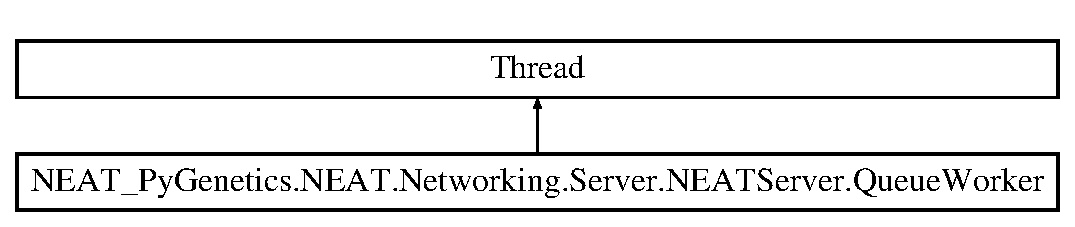
\includegraphics[height=2.000000cm]{class_n_e_a_t___py_genetics_1_1_n_e_a_t_1_1_networking_1_1_server_1_1_n_e_a_t_server_1_1_queue_worker}
\end{center}
\end{figure}
\subsection*{Public Member Functions}
\begin{DoxyCompactItemize}
\item 
def {\bfseries \+\_\+\+\_\+init\+\_\+\+\_\+}\hypertarget{class_n_e_a_t___py_genetics_1_1_n_e_a_t_1_1_networking_1_1_server_1_1_n_e_a_t_server_1_1_queue_worker_a413e2f230b433bfc4f137f1ae1a331e5}{}\label{class_n_e_a_t___py_genetics_1_1_n_e_a_t_1_1_networking_1_1_server_1_1_n_e_a_t_server_1_1_queue_worker_a413e2f230b433bfc4f137f1ae1a331e5}

\item 
def {\bfseries run} (self)\hypertarget{class_n_e_a_t___py_genetics_1_1_n_e_a_t_1_1_networking_1_1_server_1_1_n_e_a_t_server_1_1_queue_worker_a856d13880c0616f9b0c25b02788a54e3}{}\label{class_n_e_a_t___py_genetics_1_1_n_e_a_t_1_1_networking_1_1_server_1_1_n_e_a_t_server_1_1_queue_worker_a856d13880c0616f9b0c25b02788a54e3}

\end{DoxyCompactItemize}
\subsection*{Public Attributes}
\begin{DoxyCompactItemize}
\item 
{\bfseries socket}\hypertarget{class_n_e_a_t___py_genetics_1_1_n_e_a_t_1_1_networking_1_1_server_1_1_n_e_a_t_server_1_1_queue_worker_ad5eb20f5b3bfb6a6aafa945bd5103c1b}{}\label{class_n_e_a_t___py_genetics_1_1_n_e_a_t_1_1_networking_1_1_server_1_1_n_e_a_t_server_1_1_queue_worker_ad5eb20f5b3bfb6a6aafa945bd5103c1b}

\end{DoxyCompactItemize}


\subsection{Detailed Description}
\begin{DoxyVerb}A thread which operates on networking message queues
via JSONSocket in two different modes:

1. receive
The worker thread will accept JSONSocket connections,
receive dictionaries, creates command objects and inserts them
into the appropriate queue (in_queue)

2. send
The worker thread will wait for command objects to appear inside
the outgoing queue (out_queue), convert them to dictionaries
and send them to the client via a JSONSocket.
\end{DoxyVerb}
 

Definition at line 35 of file N\+E\+A\+T\+Server.\+py.



The documentation for this class was generated from the following file\+:\begin{DoxyCompactItemize}
\item 
N\+E\+A\+T/\+Networking/\+Server/N\+E\+A\+T\+Server.\+py\end{DoxyCompactItemize}

\hypertarget{class_n_e_a_t___py_genetics_1_1_n_e_a_t_1_1_error_handling_1_1_exceptions_1_1_serialization_exced8c283cc206751d1c7b7fc1791f39a64}{}\section{N\+E\+A\+T\+\_\+\+Py\+Genetics.\+N\+E\+A\+T.\+Error\+Handling.\+Exceptions.\+Serialization\+Exception.\+Serialization\+Exception Class Reference}
\label{class_n_e_a_t___py_genetics_1_1_n_e_a_t_1_1_error_handling_1_1_exceptions_1_1_serialization_exced8c283cc206751d1c7b7fc1791f39a64}\index{N\+E\+A\+T\+\_\+\+Py\+Genetics.\+N\+E\+A\+T.\+Error\+Handling.\+Exceptions.\+Serialization\+Exception.\+Serialization\+Exception@{N\+E\+A\+T\+\_\+\+Py\+Genetics.\+N\+E\+A\+T.\+Error\+Handling.\+Exceptions.\+Serialization\+Exception.\+Serialization\+Exception}}
Inheritance diagram for N\+E\+A\+T\+\_\+\+Py\+Genetics.\+N\+E\+A\+T.\+Error\+Handling.\+Exceptions.\+Serialization\+Exception.\+Serialization\+Exception\+:\begin{figure}[H]
\begin{center}
\leavevmode
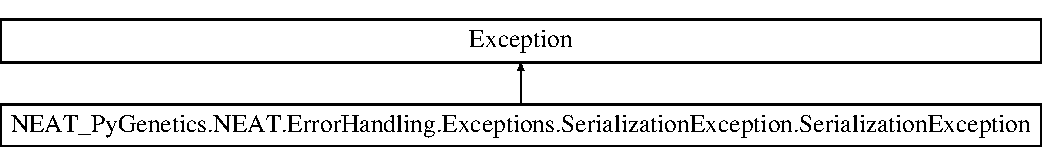
\includegraphics[height=1.978799cm]{class_n_e_a_t___py_genetics_1_1_n_e_a_t_1_1_error_handling_1_1_exceptions_1_1_serialization_exced8c283cc206751d1c7b7fc1791f39a64}
\end{center}
\end{figure}
\subsection*{Public Member Functions}
\begin{DoxyCompactItemize}
\item 
def {\bfseries \+\_\+\+\_\+init\+\_\+\+\_\+} (self, message=\char`\"{}\char`\"{}, errors=None)\hypertarget{class_n_e_a_t___py_genetics_1_1_n_e_a_t_1_1_error_handling_1_1_exceptions_1_1_serialization_exced8c283cc206751d1c7b7fc1791f39a64_ada817ecebb49fc5dc085531462eef9a0}{}\label{class_n_e_a_t___py_genetics_1_1_n_e_a_t_1_1_error_handling_1_1_exceptions_1_1_serialization_exced8c283cc206751d1c7b7fc1791f39a64_ada817ecebb49fc5dc085531462eef9a0}

\end{DoxyCompactItemize}


\subsection{Detailed Description}


Definition at line 1 of file Serialization\+Exception.\+py.



The documentation for this class was generated from the following file\+:\begin{DoxyCompactItemize}
\item 
N\+E\+A\+T/\+Error\+Handling/\+Exceptions/Serialization\+Exception.\+py\end{DoxyCompactItemize}

\hypertarget{class_n_e_a_t___py_genetics_1_1_n_e_a_t_1_1_networking_1_1_commands_1_1_set_fitness_values_comma81a16061636d0840e697e190c694b7ad}{}\section{N\+E\+A\+T\+\_\+\+Py\+Genetics.\+N\+E\+A\+T.\+Networking.\+Commands.\+Set\+Fitness\+Values\+Command.\+Set\+Fitness\+Values\+Command Class Reference}
\label{class_n_e_a_t___py_genetics_1_1_n_e_a_t_1_1_networking_1_1_commands_1_1_set_fitness_values_comma81a16061636d0840e697e190c694b7ad}\index{N\+E\+A\+T\+\_\+\+Py\+Genetics.\+N\+E\+A\+T.\+Networking.\+Commands.\+Set\+Fitness\+Values\+Command.\+Set\+Fitness\+Values\+Command@{N\+E\+A\+T\+\_\+\+Py\+Genetics.\+N\+E\+A\+T.\+Networking.\+Commands.\+Set\+Fitness\+Values\+Command.\+Set\+Fitness\+Values\+Command}}
Inheritance diagram for N\+E\+A\+T\+\_\+\+Py\+Genetics.\+N\+E\+A\+T.\+Networking.\+Commands.\+Set\+Fitness\+Values\+Command.\+Set\+Fitness\+Values\+Command\+:\begin{figure}[H]
\begin{center}
\leavevmode
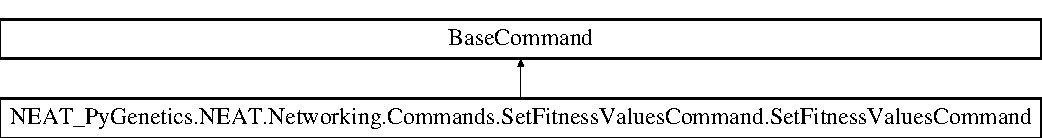
\includegraphics[height=1.851240cm]{class_n_e_a_t___py_genetics_1_1_n_e_a_t_1_1_networking_1_1_commands_1_1_set_fitness_values_comma81a16061636d0840e697e190c694b7ad}
\end{center}
\end{figure}
\subsection*{Public Member Functions}
\begin{DoxyCompactItemize}
\item 
def {\bfseries \+\_\+\+\_\+init\+\_\+\+\_\+} (self)\hypertarget{class_n_e_a_t___py_genetics_1_1_n_e_a_t_1_1_networking_1_1_commands_1_1_set_fitness_values_comma81a16061636d0840e697e190c694b7ad_af1878c6d7a7fcb3d42693ebf5ab9a8f9}{}\label{class_n_e_a_t___py_genetics_1_1_n_e_a_t_1_1_networking_1_1_commands_1_1_set_fitness_values_comma81a16061636d0840e697e190c694b7ad_af1878c6d7a7fcb3d42693ebf5ab9a8f9}

\item 
def {\bfseries set\+\_\+fitness\+\_\+values}\hypertarget{class_n_e_a_t___py_genetics_1_1_n_e_a_t_1_1_networking_1_1_commands_1_1_set_fitness_values_comma81a16061636d0840e697e190c694b7ad_ad422d62ec35756ac1375c71222e902ba}{}\label{class_n_e_a_t___py_genetics_1_1_n_e_a_t_1_1_networking_1_1_commands_1_1_set_fitness_values_comma81a16061636d0840e697e190c694b7ad_ad422d62ec35756ac1375c71222e902ba}

\item 
def {\bfseries set\+\_\+fitness\+\_\+value}\hypertarget{class_n_e_a_t___py_genetics_1_1_n_e_a_t_1_1_networking_1_1_commands_1_1_set_fitness_values_comma81a16061636d0840e697e190c694b7ad_a44c78bd4ea207b596aa62cf5e6ee5ebc}{}\label{class_n_e_a_t___py_genetics_1_1_n_e_a_t_1_1_networking_1_1_commands_1_1_set_fitness_values_comma81a16061636d0840e697e190c694b7ad_a44c78bd4ea207b596aa62cf5e6ee5ebc}

\end{DoxyCompactItemize}


\subsection{Detailed Description}


Definition at line 5 of file Set\+Fitness\+Values\+Command.\+py.



The documentation for this class was generated from the following file\+:\begin{DoxyCompactItemize}
\item 
N\+E\+A\+T/\+Networking/\+Commands/Set\+Fitness\+Values\+Command.\+py\end{DoxyCompactItemize}

\hypertarget{class_n_e_a_t___py_genetics_1_1_n_e_a_t_1_1_networking_1_1_commands_1_1_set_inputs_command_1_1_set_inputs_command}{}\section{N\+E\+A\+T\+\_\+\+Py\+Genetics.\+N\+E\+A\+T.\+Networking.\+Commands.\+Set\+Inputs\+Command.\+Set\+Inputs\+Command Class Reference}
\label{class_n_e_a_t___py_genetics_1_1_n_e_a_t_1_1_networking_1_1_commands_1_1_set_inputs_command_1_1_set_inputs_command}\index{N\+E\+A\+T\+\_\+\+Py\+Genetics.\+N\+E\+A\+T.\+Networking.\+Commands.\+Set\+Inputs\+Command.\+Set\+Inputs\+Command@{N\+E\+A\+T\+\_\+\+Py\+Genetics.\+N\+E\+A\+T.\+Networking.\+Commands.\+Set\+Inputs\+Command.\+Set\+Inputs\+Command}}
Inheritance diagram for N\+E\+A\+T\+\_\+\+Py\+Genetics.\+N\+E\+A\+T.\+Networking.\+Commands.\+Set\+Inputs\+Command.\+Set\+Inputs\+Command\+:\begin{figure}[H]
\begin{center}
\leavevmode
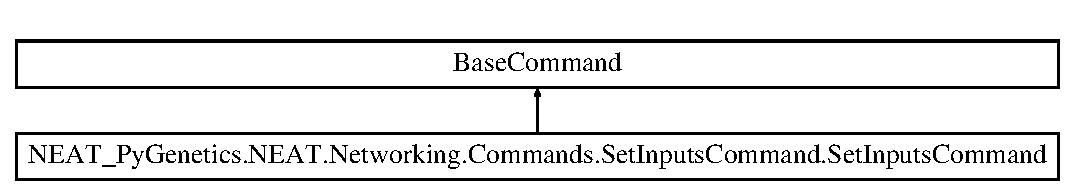
\includegraphics[height=2.000000cm]{class_n_e_a_t___py_genetics_1_1_n_e_a_t_1_1_networking_1_1_commands_1_1_set_inputs_command_1_1_set_inputs_command}
\end{center}
\end{figure}
\subsection*{Public Member Functions}
\begin{DoxyCompactItemize}
\item 
def {\bfseries \+\_\+\+\_\+init\+\_\+\+\_\+} (self)\hypertarget{class_n_e_a_t___py_genetics_1_1_n_e_a_t_1_1_networking_1_1_commands_1_1_set_inputs_command_1_1_set_inputs_command_a8976dadea27ff8c738c32b2a8c42acde}{}\label{class_n_e_a_t___py_genetics_1_1_n_e_a_t_1_1_networking_1_1_commands_1_1_set_inputs_command_1_1_set_inputs_command_a8976dadea27ff8c738c32b2a8c42acde}

\item 
def {\bfseries set\+\_\+inputs}\hypertarget{class_n_e_a_t___py_genetics_1_1_n_e_a_t_1_1_networking_1_1_commands_1_1_set_inputs_command_1_1_set_inputs_command_a610420d005c225778fa1be622cd3843a}{}\label{class_n_e_a_t___py_genetics_1_1_n_e_a_t_1_1_networking_1_1_commands_1_1_set_inputs_command_1_1_set_inputs_command_a610420d005c225778fa1be622cd3843a}

\end{DoxyCompactItemize}


\subsection{Detailed Description}


Definition at line 5 of file Set\+Inputs\+Command.\+py.



The documentation for this class was generated from the following file\+:\begin{DoxyCompactItemize}
\item 
N\+E\+A\+T/\+Networking/\+Commands/Set\+Inputs\+Command.\+py\end{DoxyCompactItemize}

\hypertarget{class_n_e_a_t___py_genetics_1_1_n_e_a_t_1_1_networking_1_1_client_1_1_simulation_client_1_1_simulation_client}{}\section{N\+E\+A\+T\+\_\+\+Py\+Genetics.\+N\+E\+A\+T.\+Networking.\+Client.\+Simulation\+Client.\+Simulation\+Client Class Reference}
\label{class_n_e_a_t___py_genetics_1_1_n_e_a_t_1_1_networking_1_1_client_1_1_simulation_client_1_1_simulation_client}\index{N\+E\+A\+T\+\_\+\+Py\+Genetics.\+N\+E\+A\+T.\+Networking.\+Client.\+Simulation\+Client.\+Simulation\+Client@{N\+E\+A\+T\+\_\+\+Py\+Genetics.\+N\+E\+A\+T.\+Networking.\+Client.\+Simulation\+Client.\+Simulation\+Client}}
Inheritance diagram for N\+E\+A\+T\+\_\+\+Py\+Genetics.\+N\+E\+A\+T.\+Networking.\+Client.\+Simulation\+Client.\+Simulation\+Client\+:\begin{figure}[H]
\begin{center}
\leavevmode
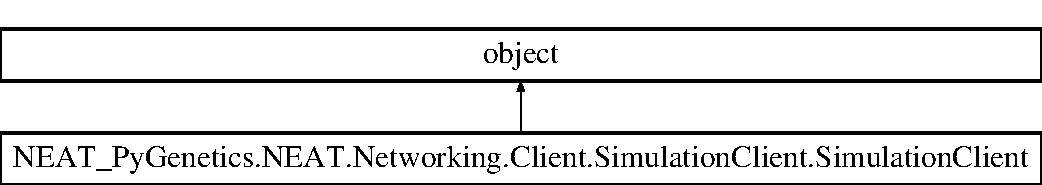
\includegraphics[height=2.000000cm]{class_n_e_a_t___py_genetics_1_1_n_e_a_t_1_1_networking_1_1_client_1_1_simulation_client_1_1_simulation_client}
\end{center}
\end{figure}
\subsection*{Public Member Functions}
\begin{DoxyCompactItemize}
\item 
def {\bfseries \+\_\+\+\_\+init\+\_\+\+\_\+} (self, server\+\_\+address, server\+\_\+port)\hypertarget{class_n_e_a_t___py_genetics_1_1_n_e_a_t_1_1_networking_1_1_client_1_1_simulation_client_1_1_simulation_client_a1c778ac890847ec7cf4f2dedab962ce9}{}\label{class_n_e_a_t___py_genetics_1_1_n_e_a_t_1_1_networking_1_1_client_1_1_simulation_client_1_1_simulation_client_a1c778ac890847ec7cf4f2dedab962ce9}

\item 
def {\bfseries announce\+\_\+session} (self, session\+\_\+id, config\+\_\+path=None, block\+\_\+size=1)\hypertarget{class_n_e_a_t___py_genetics_1_1_n_e_a_t_1_1_networking_1_1_client_1_1_simulation_client_1_1_simulation_client_a32f0a2edf3339e2d874bca161516ac18}{}\label{class_n_e_a_t___py_genetics_1_1_n_e_a_t_1_1_networking_1_1_client_1_1_simulation_client_1_1_simulation_client_a32f0a2edf3339e2d874bca161516ac18}

\item 
def {\bfseries get\+\_\+block}\hypertarget{class_n_e_a_t___py_genetics_1_1_n_e_a_t_1_1_networking_1_1_client_1_1_simulation_client_1_1_simulation_client_ad77ac994b568f19bb7468ebff9332cbc}{}\label{class_n_e_a_t___py_genetics_1_1_n_e_a_t_1_1_networking_1_1_client_1_1_simulation_client_1_1_simulation_client_ad77ac994b568f19bb7468ebff9332cbc}

\item 
def {\bfseries set\+\_\+block\+\_\+inputs}\hypertarget{class_n_e_a_t___py_genetics_1_1_n_e_a_t_1_1_networking_1_1_client_1_1_simulation_client_1_1_simulation_client_a6cb78ce85e0d06b14c4da1235ca554b0}{}\label{class_n_e_a_t___py_genetics_1_1_n_e_a_t_1_1_networking_1_1_client_1_1_simulation_client_1_1_simulation_client_a6cb78ce85e0d06b14c4da1235ca554b0}

\item 
def {\bfseries get\+\_\+block\+\_\+outputs}\hypertarget{class_n_e_a_t___py_genetics_1_1_n_e_a_t_1_1_networking_1_1_client_1_1_simulation_client_1_1_simulation_client_a9d5c043ac1439872cfcbb767e751d586}{}\label{class_n_e_a_t___py_genetics_1_1_n_e_a_t_1_1_networking_1_1_client_1_1_simulation_client_1_1_simulation_client_a9d5c043ac1439872cfcbb767e751d586}

\item 
def {\bfseries set\+\_\+fitness\+\_\+values}\hypertarget{class_n_e_a_t___py_genetics_1_1_n_e_a_t_1_1_networking_1_1_client_1_1_simulation_client_1_1_simulation_client_a30dca9ecfedc51b314579100f8fa21d4}{}\label{class_n_e_a_t___py_genetics_1_1_n_e_a_t_1_1_networking_1_1_client_1_1_simulation_client_1_1_simulation_client_a30dca9ecfedc51b314579100f8fa21d4}

\item 
def {\bfseries advance\+\_\+generation} (self)\hypertarget{class_n_e_a_t___py_genetics_1_1_n_e_a_t_1_1_networking_1_1_client_1_1_simulation_client_1_1_simulation_client_a8aa37dad9f6092178fd4b08e654829ca}{}\label{class_n_e_a_t___py_genetics_1_1_n_e_a_t_1_1_networking_1_1_client_1_1_simulation_client_1_1_simulation_client_a8aa37dad9f6092178fd4b08e654829ca}

\item 
def {\bfseries archive\+\_\+session} (self)\hypertarget{class_n_e_a_t___py_genetics_1_1_n_e_a_t_1_1_networking_1_1_client_1_1_simulation_client_1_1_simulation_client_a2b90544554ffa9c9d884f68c9e4ec01b}{}\label{class_n_e_a_t___py_genetics_1_1_n_e_a_t_1_1_networking_1_1_client_1_1_simulation_client_1_1_simulation_client_a2b90544554ffa9c9d884f68c9e4ec01b}

\end{DoxyCompactItemize}
\subsection*{Static Public Attributes}
\begin{DoxyCompactItemize}
\item 
{\bfseries command}\hypertarget{class_n_e_a_t___py_genetics_1_1_n_e_a_t_1_1_networking_1_1_client_1_1_simulation_client_1_1_simulation_client_ae492ae862d9d7a5096f16051c4b43cb0}{}\label{class_n_e_a_t___py_genetics_1_1_n_e_a_t_1_1_networking_1_1_client_1_1_simulation_client_1_1_simulation_client_ae492ae862d9d7a5096f16051c4b43cb0}

\item 
{\bfseries response}\hypertarget{class_n_e_a_t___py_genetics_1_1_n_e_a_t_1_1_networking_1_1_client_1_1_simulation_client_1_1_simulation_client_a6a2ac9e9e4603999962e160328eaffce}{}\label{class_n_e_a_t___py_genetics_1_1_n_e_a_t_1_1_networking_1_1_client_1_1_simulation_client_1_1_simulation_client_a6a2ac9e9e4603999962e160328eaffce}

\end{DoxyCompactItemize}


\subsection{Detailed Description}


Definition at line 15 of file Simulation\+Client.\+py.



The documentation for this class was generated from the following file\+:\begin{DoxyCompactItemize}
\item 
N\+E\+A\+T/\+Networking/\+Client/Simulation\+Client.\+py\end{DoxyCompactItemize}

\hypertarget{class_n_e_a_t___py_genetics_1_1_n_e_a_t_1_1_networking_1_1_server_1_1_simulation_connector_1_1_simulation_connector}{}\section{N\+E\+A\+T\+\_\+\+Py\+Genetics.\+N\+E\+A\+T.\+Networking.\+Server.\+Simulation\+Connector.\+Simulation\+Connector Class Reference}
\label{class_n_e_a_t___py_genetics_1_1_n_e_a_t_1_1_networking_1_1_server_1_1_simulation_connector_1_1_simulation_connector}\index{N\+E\+A\+T\+\_\+\+Py\+Genetics.\+N\+E\+A\+T.\+Networking.\+Server.\+Simulation\+Connector.\+Simulation\+Connector@{N\+E\+A\+T\+\_\+\+Py\+Genetics.\+N\+E\+A\+T.\+Networking.\+Server.\+Simulation\+Connector.\+Simulation\+Connector}}
Inheritance diagram for N\+E\+A\+T\+\_\+\+Py\+Genetics.\+N\+E\+A\+T.\+Networking.\+Server.\+Simulation\+Connector.\+Simulation\+Connector\+:\begin{figure}[H]
\begin{center}
\leavevmode
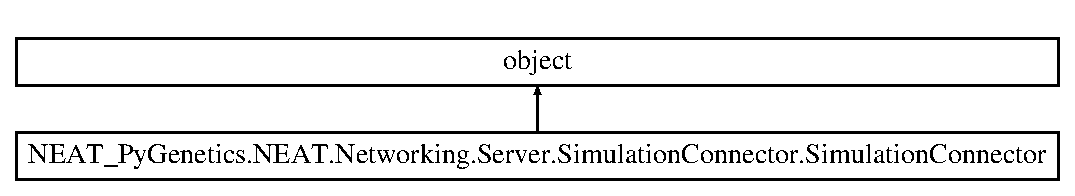
\includegraphics[height=2.000000cm]{class_n_e_a_t___py_genetics_1_1_n_e_a_t_1_1_networking_1_1_server_1_1_simulation_connector_1_1_simulation_connector}
\end{center}
\end{figure}
\subsection*{Public Member Functions}
\begin{DoxyCompactItemize}
\item 
def {\bfseries \+\_\+\+\_\+init\+\_\+\+\_\+} (self)\hypertarget{class_n_e_a_t___py_genetics_1_1_n_e_a_t_1_1_networking_1_1_server_1_1_simulation_connector_1_1_simulation_connector_a3efe4fc8a7d68cfd454fbaf0e981bee5}{}\label{class_n_e_a_t___py_genetics_1_1_n_e_a_t_1_1_networking_1_1_server_1_1_simulation_connector_1_1_simulation_connector_a3efe4fc8a7d68cfd454fbaf0e981bee5}

\item 
def \hyperlink{class_n_e_a_t___py_genetics_1_1_n_e_a_t_1_1_networking_1_1_server_1_1_simulation_connector_1_1_simulation_connector_af5849c17a1aa5ef6bc4f9e1f798fe00c}{get\+\_\+session} (self)
\item 
def {\bfseries send\+\_\+block}\hypertarget{class_n_e_a_t___py_genetics_1_1_n_e_a_t_1_1_networking_1_1_server_1_1_simulation_connector_1_1_simulation_connector_a4984c0604704e1808a51050274c7a56e}{}\label{class_n_e_a_t___py_genetics_1_1_n_e_a_t_1_1_networking_1_1_server_1_1_simulation_connector_1_1_simulation_connector_a4984c0604704e1808a51050274c7a56e}

\item 
def {\bfseries get\+\_\+block\+\_\+inputs}\hypertarget{class_n_e_a_t___py_genetics_1_1_n_e_a_t_1_1_networking_1_1_server_1_1_simulation_connector_1_1_simulation_connector_a193505d0bf3a8dfa0063b7aca22cd84b}{}\label{class_n_e_a_t___py_genetics_1_1_n_e_a_t_1_1_networking_1_1_server_1_1_simulation_connector_1_1_simulation_connector_a193505d0bf3a8dfa0063b7aca22cd84b}

\item 
def {\bfseries send\+\_\+block\+\_\+outputs}\hypertarget{class_n_e_a_t___py_genetics_1_1_n_e_a_t_1_1_networking_1_1_server_1_1_simulation_connector_1_1_simulation_connector_a82d0ed025654632c25d2241aef9024cc}{}\label{class_n_e_a_t___py_genetics_1_1_n_e_a_t_1_1_networking_1_1_server_1_1_simulation_connector_1_1_simulation_connector_a82d0ed025654632c25d2241aef9024cc}

\item 
def {\bfseries get\+\_\+fitness\+\_\+values}\hypertarget{class_n_e_a_t___py_genetics_1_1_n_e_a_t_1_1_networking_1_1_server_1_1_simulation_connector_1_1_simulation_connector_af63e36b9eb1e3dcc9d58e437d251cc35}{}\label{class_n_e_a_t___py_genetics_1_1_n_e_a_t_1_1_networking_1_1_server_1_1_simulation_connector_1_1_simulation_connector_af63e36b9eb1e3dcc9d58e437d251cc35}

\item 
def \hyperlink{class_n_e_a_t___py_genetics_1_1_n_e_a_t_1_1_networking_1_1_server_1_1_simulation_connector_1_1_simulation_connector_a5a07ea6d6971102b7dbe65e8fbaeb2c6}{get\+\_\+advance\+\_\+generation} (self)
\end{DoxyCompactItemize}
\subsection*{Static Public Attributes}
\begin{DoxyCompactItemize}
\item 
{\bfseries command}\hypertarget{class_n_e_a_t___py_genetics_1_1_n_e_a_t_1_1_networking_1_1_server_1_1_simulation_connector_1_1_simulation_connector_a2ee895f0adc1c5612da513e76337a2a1}{}\label{class_n_e_a_t___py_genetics_1_1_n_e_a_t_1_1_networking_1_1_server_1_1_simulation_connector_1_1_simulation_connector_a2ee895f0adc1c5612da513e76337a2a1}

\item 
{\bfseries acknowledged}\hypertarget{class_n_e_a_t___py_genetics_1_1_n_e_a_t_1_1_networking_1_1_server_1_1_simulation_connector_1_1_simulation_connector_a382935d414f40fe1f061eb2599aaee45}{}\label{class_n_e_a_t___py_genetics_1_1_n_e_a_t_1_1_networking_1_1_server_1_1_simulation_connector_1_1_simulation_connector_a382935d414f40fe1f061eb2599aaee45}

\item 
{\bfseries result}\hypertarget{class_n_e_a_t___py_genetics_1_1_n_e_a_t_1_1_networking_1_1_server_1_1_simulation_connector_1_1_simulation_connector_a192917886950be80d6b617d89741272e}{}\label{class_n_e_a_t___py_genetics_1_1_n_e_a_t_1_1_networking_1_1_server_1_1_simulation_connector_1_1_simulation_connector_a192917886950be80d6b617d89741272e}

\item 
{\bfseries block\+\_\+to\+\_\+send}\hypertarget{class_n_e_a_t___py_genetics_1_1_n_e_a_t_1_1_networking_1_1_server_1_1_simulation_connector_1_1_simulation_connector_acf2ca405ae294326df8c2ef7b32d7024}{}\label{class_n_e_a_t___py_genetics_1_1_n_e_a_t_1_1_networking_1_1_server_1_1_simulation_connector_1_1_simulation_connector_acf2ca405ae294326df8c2ef7b32d7024}

\item 
{\bfseries get\+\_\+command}\hypertarget{class_n_e_a_t___py_genetics_1_1_n_e_a_t_1_1_networking_1_1_server_1_1_simulation_connector_1_1_simulation_connector_a09ae391da51cbab362309cde45eee5a4}{}\label{class_n_e_a_t___py_genetics_1_1_n_e_a_t_1_1_networking_1_1_server_1_1_simulation_connector_1_1_simulation_connector_a09ae391da51cbab362309cde45eee5a4}

\item 
{\bfseries set\+\_\+command}\hypertarget{class_n_e_a_t___py_genetics_1_1_n_e_a_t_1_1_networking_1_1_server_1_1_simulation_connector_1_1_simulation_connector_ae984255e91818c23a045b807d373bf1b}{}\label{class_n_e_a_t___py_genetics_1_1_n_e_a_t_1_1_networking_1_1_server_1_1_simulation_connector_1_1_simulation_connector_ae984255e91818c23a045b807d373bf1b}

\end{DoxyCompactItemize}


\subsection{Detailed Description}
\begin{DoxyVerb}A class providing a high-level interface to
a client connected via the NEATClient.
It receives commands from NEATServer's message
queue und responds to them.
When a function from SimulationConnector is called,
the client is expected to have sent a certain command
(if there are no commands in the message queue, the Server
will wait for the next command to be received). If the
client has sent another command, or a command where
the expected parameters are not present,
NetworkProtocolException will be raised.
\end{DoxyVerb}
 

Definition at line 12 of file Simulation\+Connector.\+py.



\subsection{Member Function Documentation}
\index{N\+E\+A\+T\+\_\+\+Py\+Genetics\+::\+N\+E\+A\+T\+::\+Networking\+::\+Server\+::\+Simulation\+Connector\+::\+Simulation\+Connector@{N\+E\+A\+T\+\_\+\+Py\+Genetics\+::\+N\+E\+A\+T\+::\+Networking\+::\+Server\+::\+Simulation\+Connector\+::\+Simulation\+Connector}!get\+\_\+advance\+\_\+generation@{get\+\_\+advance\+\_\+generation}}
\index{get\+\_\+advance\+\_\+generation@{get\+\_\+advance\+\_\+generation}!N\+E\+A\+T\+\_\+\+Py\+Genetics\+::\+N\+E\+A\+T\+::\+Networking\+::\+Server\+::\+Simulation\+Connector\+::\+Simulation\+Connector@{N\+E\+A\+T\+\_\+\+Py\+Genetics\+::\+N\+E\+A\+T\+::\+Networking\+::\+Server\+::\+Simulation\+Connector\+::\+Simulation\+Connector}}
\subsubsection[{\texorpdfstring{get\+\_\+advance\+\_\+generation(self)}{get_advance_generation(self)}}]{\setlength{\rightskip}{0pt plus 5cm}def N\+E\+A\+T\+\_\+\+Py\+Genetics.\+N\+E\+A\+T.\+Networking.\+Server.\+Simulation\+Connector.\+Simulation\+Connector.\+get\+\_\+advance\+\_\+generation (
\begin{DoxyParamCaption}
\item[{}]{self, }
\item[{}]{bool}
\end{DoxyParamCaption}
)}\hypertarget{class_n_e_a_t___py_genetics_1_1_n_e_a_t_1_1_networking_1_1_server_1_1_simulation_connector_1_1_simulation_connector_a5a07ea6d6971102b7dbe65e8fbaeb2c6}{}\label{class_n_e_a_t___py_genetics_1_1_n_e_a_t_1_1_networking_1_1_server_1_1_simulation_connector_1_1_simulation_connector_a5a07ea6d6971102b7dbe65e8fbaeb2c6}
\begin{DoxyVerb}Awaits the AdvanceGeneration command to be sent by the client.
:return: A bool indicating whether the next generation should be
calculated by NEAT (True) or the current session should be archived
(False).
\end{DoxyVerb}
 

Definition at line 217 of file Simulation\+Connector.\+py.

\index{N\+E\+A\+T\+\_\+\+Py\+Genetics\+::\+N\+E\+A\+T\+::\+Networking\+::\+Server\+::\+Simulation\+Connector\+::\+Simulation\+Connector@{N\+E\+A\+T\+\_\+\+Py\+Genetics\+::\+N\+E\+A\+T\+::\+Networking\+::\+Server\+::\+Simulation\+Connector\+::\+Simulation\+Connector}!get\+\_\+session@{get\+\_\+session}}
\index{get\+\_\+session@{get\+\_\+session}!N\+E\+A\+T\+\_\+\+Py\+Genetics\+::\+N\+E\+A\+T\+::\+Networking\+::\+Server\+::\+Simulation\+Connector\+::\+Simulation\+Connector@{N\+E\+A\+T\+\_\+\+Py\+Genetics\+::\+N\+E\+A\+T\+::\+Networking\+::\+Server\+::\+Simulation\+Connector\+::\+Simulation\+Connector}}
\subsubsection[{\texorpdfstring{get\+\_\+session(self)}{get_session(self)}}]{\setlength{\rightskip}{0pt plus 5cm}def N\+E\+A\+T\+\_\+\+Py\+Genetics.\+N\+E\+A\+T.\+Networking.\+Server.\+Simulation\+Connector.\+Simulation\+Connector.\+get\+\_\+session (
\begin{DoxyParamCaption}
\item[{}]{self, }
\item[{}]{Dict, }
\item[{}]{str, }
\item[{}]{object}
\end{DoxyParamCaption}
)}\hypertarget{class_n_e_a_t___py_genetics_1_1_n_e_a_t_1_1_networking_1_1_server_1_1_simulation_connector_1_1_simulation_connector_af5849c17a1aa5ef6bc4f9e1f798fe00c}{}\label{class_n_e_a_t___py_genetics_1_1_n_e_a_t_1_1_networking_1_1_server_1_1_simulation_connector_1_1_simulation_connector_af5849c17a1aa5ef6bc4f9e1f798fe00c}
\begin{DoxyVerb}Awaits the AnnounceSession command to be sent by the client.
:return: The session parameters for the new simulation session
\end{DoxyVerb}
 

Definition at line 108 of file Simulation\+Connector.\+py.



The documentation for this class was generated from the following file\+:\begin{DoxyCompactItemize}
\item 
N\+E\+A\+T/\+Networking/\+Server/Simulation\+Connector.\+py\end{DoxyCompactItemize}

\hypertarget{class_n_e_a_t___py_genetics_1_1_n_e_a_t_1_1_genome_structures_1_1_simulation_structure_1_1_simul922750a261fa1d0ca70a732923057496}{}\section{N\+E\+A\+T\+\_\+\+Py\+Genetics.\+N\+E\+A\+T.\+Genome\+Structures.\+Simulation\+Structure.\+Simulation\+Genome.\+Simulation\+Genome Class Reference}
\label{class_n_e_a_t___py_genetics_1_1_n_e_a_t_1_1_genome_structures_1_1_simulation_structure_1_1_simul922750a261fa1d0ca70a732923057496}\index{N\+E\+A\+T\+\_\+\+Py\+Genetics.\+N\+E\+A\+T.\+Genome\+Structures.\+Simulation\+Structure.\+Simulation\+Genome.\+Simulation\+Genome@{N\+E\+A\+T\+\_\+\+Py\+Genetics.\+N\+E\+A\+T.\+Genome\+Structures.\+Simulation\+Structure.\+Simulation\+Genome.\+Simulation\+Genome}}
Inheritance diagram for N\+E\+A\+T\+\_\+\+Py\+Genetics.\+N\+E\+A\+T.\+Genome\+Structures.\+Simulation\+Structure.\+Simulation\+Genome.\+Simulation\+Genome\+:\begin{figure}[H]
\begin{center}
\leavevmode
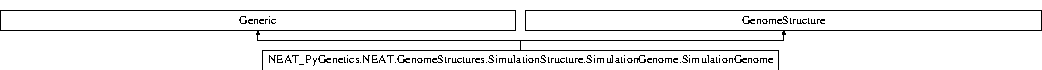
\includegraphics[height=0.939597cm]{class_n_e_a_t___py_genetics_1_1_n_e_a_t_1_1_genome_structures_1_1_simulation_structure_1_1_simul922750a261fa1d0ca70a732923057496}
\end{center}
\end{figure}
\subsection*{Public Member Functions}
\begin{DoxyCompactItemize}
\item 
def {\bfseries \+\_\+\+\_\+init\+\_\+\+\_\+}\hypertarget{class_n_e_a_t___py_genetics_1_1_n_e_a_t_1_1_genome_structures_1_1_simulation_structure_1_1_simul922750a261fa1d0ca70a732923057496_a9e3d21a710e6b90ca8d6332fbdc8faa2}{}\label{class_n_e_a_t___py_genetics_1_1_n_e_a_t_1_1_genome_structures_1_1_simulation_structure_1_1_simul922750a261fa1d0ca70a732923057496_a9e3d21a710e6b90ca8d6332fbdc8faa2}

\item 
def \hyperlink{class_n_e_a_t___py_genetics_1_1_n_e_a_t_1_1_genome_structures_1_1_simulation_structure_1_1_simul922750a261fa1d0ca70a732923057496_af8bbfbec0e15a55d7a889ba9859f034a}{output} (self)
\item 
def {\bfseries calculate\+\_\+step}\hypertarget{class_n_e_a_t___py_genetics_1_1_n_e_a_t_1_1_genome_structures_1_1_simulation_structure_1_1_simul922750a261fa1d0ca70a732923057496_ae35fc2d42a8f79cf1cf7cf65b40910b6}{}\label{class_n_e_a_t___py_genetics_1_1_n_e_a_t_1_1_genome_structures_1_1_simulation_structure_1_1_simul922750a261fa1d0ca70a732923057496_ae35fc2d42a8f79cf1cf7cf65b40910b6}

\end{DoxyCompactItemize}
\subsection*{Static Public Attributes}
\begin{DoxyCompactItemize}
\item 
{\bfseries cycle\+\_\+nodes}\hypertarget{class_n_e_a_t___py_genetics_1_1_n_e_a_t_1_1_genome_structures_1_1_simulation_structure_1_1_simul922750a261fa1d0ca70a732923057496_aa650dc24f64c63322197e5eabd879453}{}\label{class_n_e_a_t___py_genetics_1_1_n_e_a_t_1_1_genome_structures_1_1_simulation_structure_1_1_simul922750a261fa1d0ca70a732923057496_aa650dc24f64c63322197e5eabd879453}

\item 
{\bfseries hidden\+\_\+layer}\hypertarget{class_n_e_a_t___py_genetics_1_1_n_e_a_t_1_1_genome_structures_1_1_simulation_structure_1_1_simul922750a261fa1d0ca70a732923057496_a66d27e8ed15eb8473d63728d6fa046fe}{}\label{class_n_e_a_t___py_genetics_1_1_n_e_a_t_1_1_genome_structures_1_1_simulation_structure_1_1_simul922750a261fa1d0ca70a732923057496_a66d27e8ed15eb8473d63728d6fa046fe}

\item 
{\bfseries closes\+\_\+circle}\hypertarget{class_n_e_a_t___py_genetics_1_1_n_e_a_t_1_1_genome_structures_1_1_simulation_structure_1_1_simul922750a261fa1d0ca70a732923057496_a246a2949988d817f3ba2e5a27ce0cb26}{}\label{class_n_e_a_t___py_genetics_1_1_n_e_a_t_1_1_genome_structures_1_1_simulation_structure_1_1_simul922750a261fa1d0ca70a732923057496_a246a2949988d817f3ba2e5a27ce0cb26}

\item 
{\bfseries source}\hypertarget{class_n_e_a_t___py_genetics_1_1_n_e_a_t_1_1_genome_structures_1_1_simulation_structure_1_1_simul922750a261fa1d0ca70a732923057496_ac4b5b345246df8c26156052e19d88dc3}{}\label{class_n_e_a_t___py_genetics_1_1_n_e_a_t_1_1_genome_structures_1_1_simulation_structure_1_1_simul922750a261fa1d0ca70a732923057496_ac4b5b345246df8c26156052e19d88dc3}

\item 
{\bfseries target}\hypertarget{class_n_e_a_t___py_genetics_1_1_n_e_a_t_1_1_genome_structures_1_1_simulation_structure_1_1_simul922750a261fa1d0ca70a732923057496_ac175e1e9455296d28d7486373e2546c7}{}\label{class_n_e_a_t___py_genetics_1_1_n_e_a_t_1_1_genome_structures_1_1_simulation_structure_1_1_simul922750a261fa1d0ca70a732923057496_ac175e1e9455296d28d7486373e2546c7}

\item 
{\bfseries value}\hypertarget{class_n_e_a_t___py_genetics_1_1_n_e_a_t_1_1_genome_structures_1_1_simulation_structure_1_1_simul922750a261fa1d0ca70a732923057496_a27b218236fdf7a6526bdddef382a38e9}{}\label{class_n_e_a_t___py_genetics_1_1_n_e_a_t_1_1_genome_structures_1_1_simulation_structure_1_1_simul922750a261fa1d0ca70a732923057496_a27b218236fdf7a6526bdddef382a38e9}

\end{DoxyCompactItemize}


\subsection{Detailed Description}
\begin{DoxyVerb}The SimulationGenome is a structural representation of a genome's genepool.
It is optimized for the purpose of simulating a neural network and is gene-
rated from a given StorageGenome.

Attributes:
    _gene_repository:
        Access to information about the node ids in the StorageGenome
    _output:
        Contains the results of the last calculation process.
    _input_layer:
        A set of Nodes as the input layer. These are identical in number and
         ids with the input ids in the StorageGenome.
    _output_layer:
        A set of Nodes as the output layer. These are identical in number
        and ids with the output ids in the StorageGenome.
    _hidden_layer:
        A hidden layer. This consists of a list of nodes which are calcula-
        ted in the order of the list. This list is taken from the topologi-
        cally sorted node list in the given StorageGenome's AnalysisResult.
        So to ensure a functioning neural network, that list has to be cor-
        rect.
    _cycle_nodes:
        A list of CycleNodes, topologically sorted (like the hidden layer).
        These are nodes that have outgoing links that close a cycle. These
        nodes have to be treated separately, because the cycle closing edges
        have to be calculated first. For this initial calculation the last
        calculation value is used as the outgoing base value. If the genome
        was not simulated yet. a default value is used as the initial value.

Usage:
    insert StorageGenome
    call calculate_step
    have fun
\end{DoxyVerb}
 

Definition at line 13 of file Simulation\+Genome.\+py.



\subsection{Member Function Documentation}
\index{N\+E\+A\+T\+\_\+\+Py\+Genetics\+::\+N\+E\+A\+T\+::\+Genome\+Structures\+::\+Simulation\+Structure\+::\+Simulation\+Genome\+::\+Simulation\+Genome@{N\+E\+A\+T\+\_\+\+Py\+Genetics\+::\+N\+E\+A\+T\+::\+Genome\+Structures\+::\+Simulation\+Structure\+::\+Simulation\+Genome\+::\+Simulation\+Genome}!output@{output}}
\index{output@{output}!N\+E\+A\+T\+\_\+\+Py\+Genetics\+::\+N\+E\+A\+T\+::\+Genome\+Structures\+::\+Simulation\+Structure\+::\+Simulation\+Genome\+::\+Simulation\+Genome@{N\+E\+A\+T\+\_\+\+Py\+Genetics\+::\+N\+E\+A\+T\+::\+Genome\+Structures\+::\+Simulation\+Structure\+::\+Simulation\+Genome\+::\+Simulation\+Genome}}
\subsubsection[{\texorpdfstring{output(self)}{output(self)}}]{\setlength{\rightskip}{0pt plus 5cm}def N\+E\+A\+T\+\_\+\+Py\+Genetics.\+N\+E\+A\+T.\+Genome\+Structures.\+Simulation\+Structure.\+Simulation\+Genome.\+Simulation\+Genome.\+output (
\begin{DoxyParamCaption}
\item[{}]{self, }
\item[{}]{Dict, }
\item[{}]{str, }
\item[{}]{Fraction}
\end{DoxyParamCaption}
)}\hypertarget{class_n_e_a_t___py_genetics_1_1_n_e_a_t_1_1_genome_structures_1_1_simulation_structure_1_1_simul922750a261fa1d0ca70a732923057496_af8bbfbec0e15a55d7a889ba9859f034a}{}\label{class_n_e_a_t___py_genetics_1_1_n_e_a_t_1_1_genome_structures_1_1_simulation_structure_1_1_simul922750a261fa1d0ca70a732923057496_af8bbfbec0e15a55d7a889ba9859f034a}
\begin{DoxyVerb}:return: Dict of the output nodes' values of the form label:value
\end{DoxyVerb}
 

Definition at line 142 of file Simulation\+Genome.\+py.



The documentation for this class was generated from the following file\+:\begin{DoxyCompactItemize}
\item 
N\+E\+A\+T/\+Genome\+Structures/\+Simulation\+Structure/Simulation\+Genome.\+py\end{DoxyCompactItemize}

\hypertarget{class_n_e_a_t___py_genetics_1_1_n_e_a_t_1_1_simulator_1_1_simulator_1_1_simulator}{}\section{N\+E\+A\+T\+\_\+\+Py\+Genetics.\+N\+E\+A\+T.\+Simulator.\+Simulator.\+Simulator Class Reference}
\label{class_n_e_a_t___py_genetics_1_1_n_e_a_t_1_1_simulator_1_1_simulator_1_1_simulator}\index{N\+E\+A\+T\+\_\+\+Py\+Genetics.\+N\+E\+A\+T.\+Simulator.\+Simulator.\+Simulator@{N\+E\+A\+T\+\_\+\+Py\+Genetics.\+N\+E\+A\+T.\+Simulator.\+Simulator.\+Simulator}}
Inheritance diagram for N\+E\+A\+T\+\_\+\+Py\+Genetics.\+N\+E\+A\+T.\+Simulator.\+Simulator.\+Simulator\+:\begin{figure}[H]
\begin{center}
\leavevmode
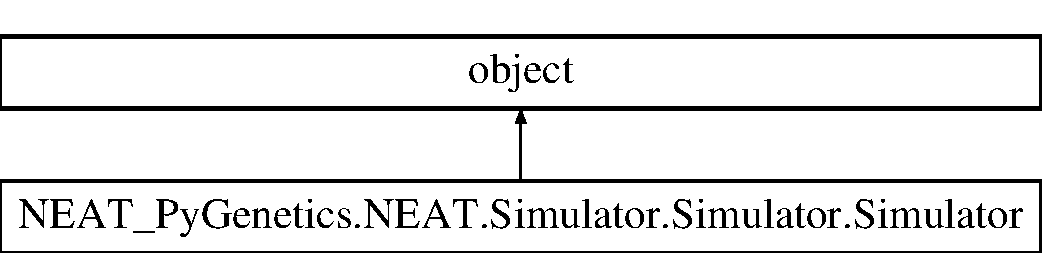
\includegraphics[height=2.000000cm]{class_n_e_a_t___py_genetics_1_1_n_e_a_t_1_1_simulator_1_1_simulator_1_1_simulator}
\end{center}
\end{figure}
\subsection*{Public Member Functions}
\begin{DoxyCompactItemize}
\item 
def {\bfseries \+\_\+\+\_\+init\+\_\+\+\_\+}\hypertarget{class_n_e_a_t___py_genetics_1_1_n_e_a_t_1_1_simulator_1_1_simulator_1_1_simulator_ab768445b7d9b16282919f062e0a42761}{}\label{class_n_e_a_t___py_genetics_1_1_n_e_a_t_1_1_simulator_1_1_simulator_1_1_simulator_ab768445b7d9b16282919f062e0a42761}

\item 
def {\bfseries simulate\+\_\+genome}\hypertarget{class_n_e_a_t___py_genetics_1_1_n_e_a_t_1_1_simulator_1_1_simulator_1_1_simulator_a0e362a7174cae20d0a23b69109ac15bc}{}\label{class_n_e_a_t___py_genetics_1_1_n_e_a_t_1_1_simulator_1_1_simulator_1_1_simulator_a0e362a7174cae20d0a23b69109ac15bc}

\end{DoxyCompactItemize}
\subsection*{Static Public Attributes}
\begin{DoxyCompactItemize}
\item 
{\bfseries simulation\+\_\+genome}\hypertarget{class_n_e_a_t___py_genetics_1_1_n_e_a_t_1_1_simulator_1_1_simulator_1_1_simulator_abbacbfee6def9b5025447526cfb6152d}{}\label{class_n_e_a_t___py_genetics_1_1_n_e_a_t_1_1_simulator_1_1_simulator_1_1_simulator_abbacbfee6def9b5025447526cfb6152d}

\item 
{\bfseries inputs}\hypertarget{class_n_e_a_t___py_genetics_1_1_n_e_a_t_1_1_simulator_1_1_simulator_1_1_simulator_a6ebf16f89e5a3f48064b85f3acd0c9e9}{}\label{class_n_e_a_t___py_genetics_1_1_n_e_a_t_1_1_simulator_1_1_simulator_1_1_simulator_a6ebf16f89e5a3f48064b85f3acd0c9e9}

\end{DoxyCompactItemize}


\subsection{Detailed Description}


Definition at line 9 of file Simulator.\+py.



The documentation for this class was generated from the following file\+:\begin{DoxyCompactItemize}
\item 
N\+E\+A\+T/\+Simulator/Simulator.\+py\end{DoxyCompactItemize}

\hypertarget{class_n_e_a_t___py_genetics_1_1_n_e_a_t_1_1_error_handling_1_1_exceptions_1_1_socket_already_usec2845100a8624939d4f1ab320dc8a73f}{}\section{N\+E\+A\+T\+\_\+\+Py\+Genetics.\+N\+E\+A\+T.\+Error\+Handling.\+Exceptions.\+Socket\+Already\+Used\+Exception.\+Socket\+Already\+Used\+Exception Class Reference}
\label{class_n_e_a_t___py_genetics_1_1_n_e_a_t_1_1_error_handling_1_1_exceptions_1_1_socket_already_usec2845100a8624939d4f1ab320dc8a73f}\index{N\+E\+A\+T\+\_\+\+Py\+Genetics.\+N\+E\+A\+T.\+Error\+Handling.\+Exceptions.\+Socket\+Already\+Used\+Exception.\+Socket\+Already\+Used\+Exception@{N\+E\+A\+T\+\_\+\+Py\+Genetics.\+N\+E\+A\+T.\+Error\+Handling.\+Exceptions.\+Socket\+Already\+Used\+Exception.\+Socket\+Already\+Used\+Exception}}
Inheritance diagram for N\+E\+A\+T\+\_\+\+Py\+Genetics.\+N\+E\+A\+T.\+Error\+Handling.\+Exceptions.\+Socket\+Already\+Used\+Exception.\+Socket\+Already\+Used\+Exception\+:\begin{figure}[H]
\begin{center}
\leavevmode
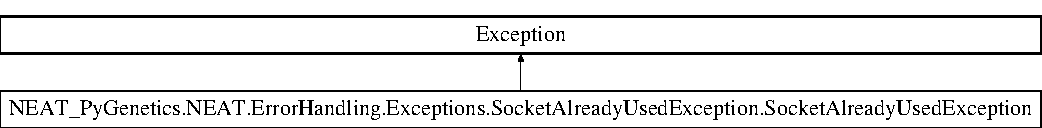
\includegraphics[height=1.723077cm]{class_n_e_a_t___py_genetics_1_1_n_e_a_t_1_1_error_handling_1_1_exceptions_1_1_socket_already_usec2845100a8624939d4f1ab320dc8a73f}
\end{center}
\end{figure}
\subsection*{Public Member Functions}
\begin{DoxyCompactItemize}
\item 
def {\bfseries \+\_\+\+\_\+init\+\_\+\+\_\+} (self, message=\char`\"{}\char`\"{}, errors=None)\hypertarget{class_n_e_a_t___py_genetics_1_1_n_e_a_t_1_1_error_handling_1_1_exceptions_1_1_socket_already_usec2845100a8624939d4f1ab320dc8a73f_aa78052a441ad0d25947f06f3ed625c1c}{}\label{class_n_e_a_t___py_genetics_1_1_n_e_a_t_1_1_error_handling_1_1_exceptions_1_1_socket_already_usec2845100a8624939d4f1ab320dc8a73f_aa78052a441ad0d25947f06f3ed625c1c}

\end{DoxyCompactItemize}


\subsection{Detailed Description}


Definition at line 1 of file Socket\+Already\+Used\+Exception.\+py.



The documentation for this class was generated from the following file\+:\begin{DoxyCompactItemize}
\item 
N\+E\+A\+T/\+Error\+Handling/\+Exceptions/Socket\+Already\+Used\+Exception.\+py\end{DoxyCompactItemize}

\hypertarget{class_n_e_a_t___py_genetics_1_1_n_e_a_t_1_1_error_handling_1_1_exceptions_1_1_socket_runtime_exc1cc17ff15ee3bc97d249f00c72f41b97}{}\section{N\+E\+A\+T\+\_\+\+Py\+Genetics.\+N\+E\+A\+T.\+Error\+Handling.\+Exceptions.\+Socket\+Runtime\+Exception.\+Socket\+Runtime\+Exception Class Reference}
\label{class_n_e_a_t___py_genetics_1_1_n_e_a_t_1_1_error_handling_1_1_exceptions_1_1_socket_runtime_exc1cc17ff15ee3bc97d249f00c72f41b97}\index{N\+E\+A\+T\+\_\+\+Py\+Genetics.\+N\+E\+A\+T.\+Error\+Handling.\+Exceptions.\+Socket\+Runtime\+Exception.\+Socket\+Runtime\+Exception@{N\+E\+A\+T\+\_\+\+Py\+Genetics.\+N\+E\+A\+T.\+Error\+Handling.\+Exceptions.\+Socket\+Runtime\+Exception.\+Socket\+Runtime\+Exception}}
Inheritance diagram for N\+E\+A\+T\+\_\+\+Py\+Genetics.\+N\+E\+A\+T.\+Error\+Handling.\+Exceptions.\+Socket\+Runtime\+Exception.\+Socket\+Runtime\+Exception\+:\begin{figure}[H]
\begin{center}
\leavevmode
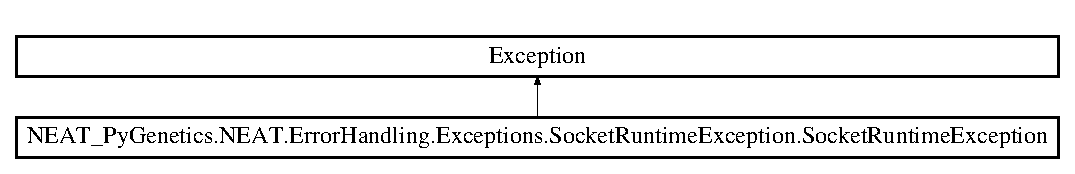
\includegraphics[height=1.891892cm]{class_n_e_a_t___py_genetics_1_1_n_e_a_t_1_1_error_handling_1_1_exceptions_1_1_socket_runtime_exc1cc17ff15ee3bc97d249f00c72f41b97}
\end{center}
\end{figure}
\subsection*{Public Member Functions}
\begin{DoxyCompactItemize}
\item 
def {\bfseries \+\_\+\+\_\+init\+\_\+\+\_\+} (self, message=\char`\"{}\char`\"{}, errors=None)\hypertarget{class_n_e_a_t___py_genetics_1_1_n_e_a_t_1_1_error_handling_1_1_exceptions_1_1_socket_runtime_exc1cc17ff15ee3bc97d249f00c72f41b97_a747071f76bd0ecd08342e4ac9d7a5e33}{}\label{class_n_e_a_t___py_genetics_1_1_n_e_a_t_1_1_error_handling_1_1_exceptions_1_1_socket_runtime_exc1cc17ff15ee3bc97d249f00c72f41b97_a747071f76bd0ecd08342e4ac9d7a5e33}

\end{DoxyCompactItemize}


\subsection{Detailed Description}


Definition at line 1 of file Socket\+Runtime\+Exception.\+py.



The documentation for this class was generated from the following file\+:\begin{DoxyCompactItemize}
\item 
N\+E\+A\+T/\+Error\+Handling/\+Exceptions/Socket\+Runtime\+Exception.\+py\end{DoxyCompactItemize}

\hypertarget{class_n_e_a_t___py_genetics_1_1_n_e_a_t_1_1_error_handling_1_1_startup_check_1_1_startup_check}{}\section{N\+E\+A\+T\+\_\+\+Py\+Genetics.\+N\+E\+A\+T.\+Error\+Handling.\+Startup\+Check.\+Startup\+Check Class Reference}
\label{class_n_e_a_t___py_genetics_1_1_n_e_a_t_1_1_error_handling_1_1_startup_check_1_1_startup_check}\index{N\+E\+A\+T\+\_\+\+Py\+Genetics.\+N\+E\+A\+T.\+Error\+Handling.\+Startup\+Check.\+Startup\+Check@{N\+E\+A\+T\+\_\+\+Py\+Genetics.\+N\+E\+A\+T.\+Error\+Handling.\+Startup\+Check.\+Startup\+Check}}
Inheritance diagram for N\+E\+A\+T\+\_\+\+Py\+Genetics.\+N\+E\+A\+T.\+Error\+Handling.\+Startup\+Check.\+Startup\+Check\+:\begin{figure}[H]
\begin{center}
\leavevmode
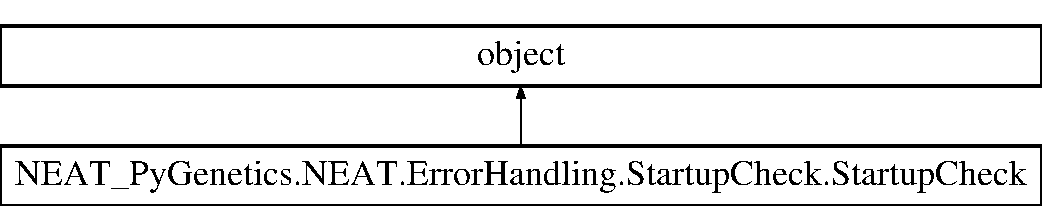
\includegraphics[height=2.000000cm]{class_n_e_a_t___py_genetics_1_1_n_e_a_t_1_1_error_handling_1_1_startup_check_1_1_startup_check}
\end{center}
\end{figure}
\subsection*{Public Member Functions}
\begin{DoxyCompactItemize}
\item 
def {\bfseries \+\_\+\+\_\+init\+\_\+\+\_\+} (self)\hypertarget{class_n_e_a_t___py_genetics_1_1_n_e_a_t_1_1_error_handling_1_1_startup_check_1_1_startup_check_a1e599ee38990fc5249559baf65685459}{}\label{class_n_e_a_t___py_genetics_1_1_n_e_a_t_1_1_error_handling_1_1_startup_check_1_1_startup_check_a1e599ee38990fc5249559baf65685459}

\item 
def {\bfseries run} (self)\hypertarget{class_n_e_a_t___py_genetics_1_1_n_e_a_t_1_1_error_handling_1_1_startup_check_1_1_startup_check_a03356f117dc673d35d69882ecabad2a3}{}\label{class_n_e_a_t___py_genetics_1_1_n_e_a_t_1_1_error_handling_1_1_startup_check_1_1_startup_check_a03356f117dc673d35d69882ecabad2a3}

\end{DoxyCompactItemize}
\subsection*{Public Attributes}
\begin{DoxyCompactItemize}
\item 
{\bfseries con}\hypertarget{class_n_e_a_t___py_genetics_1_1_n_e_a_t_1_1_error_handling_1_1_startup_check_1_1_startup_check_afca8d845c7a7796c0963e0d49ec96786}{}\label{class_n_e_a_t___py_genetics_1_1_n_e_a_t_1_1_error_handling_1_1_startup_check_1_1_startup_check_afca8d845c7a7796c0963e0d49ec96786}

\item 
{\bfseries rep}\hypertarget{class_n_e_a_t___py_genetics_1_1_n_e_a_t_1_1_error_handling_1_1_startup_check_1_1_startup_check_a9defc0bb9535a560af330658f89337ac}{}\label{class_n_e_a_t___py_genetics_1_1_n_e_a_t_1_1_error_handling_1_1_startup_check_1_1_startup_check_a9defc0bb9535a560af330658f89337ac}

\end{DoxyCompactItemize}


\subsection{Detailed Description}


Definition at line 6 of file Startup\+Check.\+py.



The documentation for this class was generated from the following file\+:\begin{DoxyCompactItemize}
\item 
N\+E\+A\+T/\+Error\+Handling/Startup\+Check.\+py\end{DoxyCompactItemize}

\hypertarget{class_n_e_a_t___py_genetics_1_1_n_e_a_t_1_1_error_handling_1_1_exceptions_1_1_startup_check_exce2a8a81d294d367a07fcb941ca1614ae5}{}\section{N\+E\+A\+T\+\_\+\+Py\+Genetics.\+N\+E\+A\+T.\+Error\+Handling.\+Exceptions.\+Startup\+Check\+Exception.\+Startup\+Check\+Exception Class Reference}
\label{class_n_e_a_t___py_genetics_1_1_n_e_a_t_1_1_error_handling_1_1_exceptions_1_1_startup_check_exce2a8a81d294d367a07fcb941ca1614ae5}\index{N\+E\+A\+T\+\_\+\+Py\+Genetics.\+N\+E\+A\+T.\+Error\+Handling.\+Exceptions.\+Startup\+Check\+Exception.\+Startup\+Check\+Exception@{N\+E\+A\+T\+\_\+\+Py\+Genetics.\+N\+E\+A\+T.\+Error\+Handling.\+Exceptions.\+Startup\+Check\+Exception.\+Startup\+Check\+Exception}}
Inheritance diagram for N\+E\+A\+T\+\_\+\+Py\+Genetics.\+N\+E\+A\+T.\+Error\+Handling.\+Exceptions.\+Startup\+Check\+Exception.\+Startup\+Check\+Exception\+:\begin{figure}[H]
\begin{center}
\leavevmode
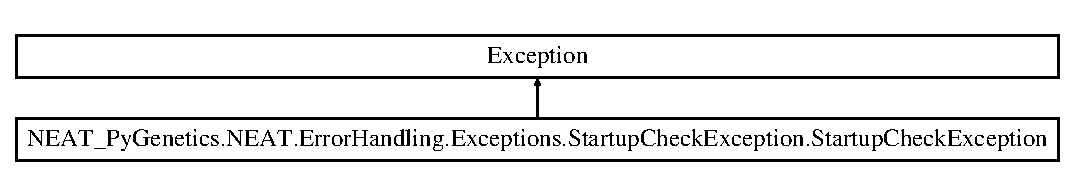
\includegraphics[height=1.931034cm]{class_n_e_a_t___py_genetics_1_1_n_e_a_t_1_1_error_handling_1_1_exceptions_1_1_startup_check_exce2a8a81d294d367a07fcb941ca1614ae5}
\end{center}
\end{figure}
\subsection*{Public Member Functions}
\begin{DoxyCompactItemize}
\item 
def {\bfseries \+\_\+\+\_\+init\+\_\+\+\_\+} (self, message=\char`\"{}\char`\"{}, errors=None)\hypertarget{class_n_e_a_t___py_genetics_1_1_n_e_a_t_1_1_error_handling_1_1_exceptions_1_1_startup_check_exce2a8a81d294d367a07fcb941ca1614ae5_a39cbd39c3a77f3acc9c3feb3bfb84d7e}{}\label{class_n_e_a_t___py_genetics_1_1_n_e_a_t_1_1_error_handling_1_1_exceptions_1_1_startup_check_exce2a8a81d294d367a07fcb941ca1614ae5_a39cbd39c3a77f3acc9c3feb3bfb84d7e}

\end{DoxyCompactItemize}


\subsection{Detailed Description}


Definition at line 1 of file Startup\+Check\+Exception.\+py.



The documentation for this class was generated from the following file\+:\begin{DoxyCompactItemize}
\item 
N\+E\+A\+T/\+Error\+Handling/\+Exceptions/Startup\+Check\+Exception.\+py\end{DoxyCompactItemize}

\hypertarget{class_n_e_a_t___py_genetics_1_1_n_e_a_t_1_1_genome_structures_1_1_storage_structure_1_1_storage_genome_1_1_storage_genome}{}\section{N\+E\+A\+T\+\_\+\+Py\+Genetics.\+N\+E\+A\+T.\+Genome\+Structures.\+Storage\+Structure.\+Storage\+Genome.\+Storage\+Genome Class Reference}
\label{class_n_e_a_t___py_genetics_1_1_n_e_a_t_1_1_genome_structures_1_1_storage_structure_1_1_storage_genome_1_1_storage_genome}\index{N\+E\+A\+T\+\_\+\+Py\+Genetics.\+N\+E\+A\+T.\+Genome\+Structures.\+Storage\+Structure.\+Storage\+Genome.\+Storage\+Genome@{N\+E\+A\+T\+\_\+\+Py\+Genetics.\+N\+E\+A\+T.\+Genome\+Structures.\+Storage\+Structure.\+Storage\+Genome.\+Storage\+Genome}}
Inheritance diagram for N\+E\+A\+T\+\_\+\+Py\+Genetics.\+N\+E\+A\+T.\+Genome\+Structures.\+Storage\+Structure.\+Storage\+Genome.\+Storage\+Genome\+:\begin{figure}[H]
\begin{center}
\leavevmode
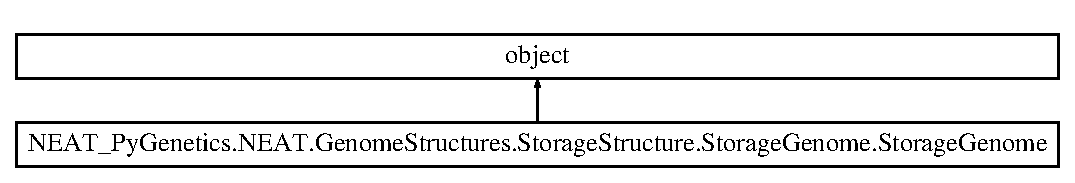
\includegraphics[height=2.000000cm]{class_n_e_a_t___py_genetics_1_1_n_e_a_t_1_1_genome_structures_1_1_storage_structure_1_1_storage_genome_1_1_storage_genome}
\end{center}
\end{figure}
\subsection*{Public Member Functions}
\begin{DoxyCompactItemize}
\item 
def {\bfseries \+\_\+\+\_\+init\+\_\+\+\_\+}\hypertarget{class_n_e_a_t___py_genetics_1_1_n_e_a_t_1_1_genome_structures_1_1_storage_structure_1_1_storage_genome_1_1_storage_genome_a8b7615cf97ad4ce4c3805ecde57637c8}{}\label{class_n_e_a_t___py_genetics_1_1_n_e_a_t_1_1_genome_structures_1_1_storage_structure_1_1_storage_genome_1_1_storage_genome_a8b7615cf97ad4ce4c3805ecde57637c8}

\item 
def {\bfseries \+\_\+\+\_\+eq\+\_\+\+\_\+}\hypertarget{class_n_e_a_t___py_genetics_1_1_n_e_a_t_1_1_genome_structures_1_1_storage_structure_1_1_storage_genome_1_1_storage_genome_a0d0ae3acf7162d05cb40fe5eaff9ada9}{}\label{class_n_e_a_t___py_genetics_1_1_n_e_a_t_1_1_genome_structures_1_1_storage_structure_1_1_storage_genome_1_1_storage_genome_a0d0ae3acf7162d05cb40fe5eaff9ada9}

\item 
def {\bfseries genome\+\_\+id} (self)\hypertarget{class_n_e_a_t___py_genetics_1_1_n_e_a_t_1_1_genome_structures_1_1_storage_structure_1_1_storage_genome_1_1_storage_genome_a536876e28c6ee27477de23a369e11daa}{}\label{class_n_e_a_t___py_genetics_1_1_n_e_a_t_1_1_genome_structures_1_1_storage_structure_1_1_storage_genome_1_1_storage_genome_a536876e28c6ee27477de23a369e11daa}

\end{DoxyCompactItemize}
\subsection*{Static Public Attributes}
\begin{DoxyCompactItemize}
\item 
{\bfseries is\+\_\+alive}\hypertarget{class_n_e_a_t___py_genetics_1_1_n_e_a_t_1_1_genome_structures_1_1_storage_structure_1_1_storage_genome_1_1_storage_genome_ae1e47996623ce538b3450f2415d57bc3}{}\label{class_n_e_a_t___py_genetics_1_1_n_e_a_t_1_1_genome_structures_1_1_storage_structure_1_1_storage_genome_1_1_storage_genome_ae1e47996623ce538b3450f2415d57bc3}

\item 
{\bfseries fitness}\hypertarget{class_n_e_a_t___py_genetics_1_1_n_e_a_t_1_1_genome_structures_1_1_storage_structure_1_1_storage_genome_1_1_storage_genome_a919c35fa0dfc5d4a81b008bef83c3ac9}{}\label{class_n_e_a_t___py_genetics_1_1_n_e_a_t_1_1_genome_structures_1_1_storage_structure_1_1_storage_genome_1_1_storage_genome_a919c35fa0dfc5d4a81b008bef83c3ac9}

\item 
{\bfseries inputs}\hypertarget{class_n_e_a_t___py_genetics_1_1_n_e_a_t_1_1_genome_structures_1_1_storage_structure_1_1_storage_genome_1_1_storage_genome_ad0bd7b5a391f6df7f56f60294fee0a00}{}\label{class_n_e_a_t___py_genetics_1_1_n_e_a_t_1_1_genome_structures_1_1_storage_structure_1_1_storage_genome_1_1_storage_genome_ad0bd7b5a391f6df7f56f60294fee0a00}

\item 
{\bfseries outputs}\hypertarget{class_n_e_a_t___py_genetics_1_1_n_e_a_t_1_1_genome_structures_1_1_storage_structure_1_1_storage_genome_1_1_storage_genome_a69f429018a927d4919d4468054cf49ea}{}\label{class_n_e_a_t___py_genetics_1_1_n_e_a_t_1_1_genome_structures_1_1_storage_structure_1_1_storage_genome_1_1_storage_genome_a69f429018a927d4919d4468054cf49ea}

\item 
{\bfseries genes}\hypertarget{class_n_e_a_t___py_genetics_1_1_n_e_a_t_1_1_genome_structures_1_1_storage_structure_1_1_storage_genome_1_1_storage_genome_a82003c70917d4c96053c6cea930383ce}{}\label{class_n_e_a_t___py_genetics_1_1_n_e_a_t_1_1_genome_structures_1_1_storage_structure_1_1_storage_genome_1_1_storage_genome_a82003c70917d4c96053c6cea930383ce}

\item 
{\bfseries analysis\+\_\+result}\hypertarget{class_n_e_a_t___py_genetics_1_1_n_e_a_t_1_1_genome_structures_1_1_storage_structure_1_1_storage_genome_1_1_storage_genome_a4ed1621581430cdf5791c33d1c2f6ac2}{}\label{class_n_e_a_t___py_genetics_1_1_n_e_a_t_1_1_genome_structures_1_1_storage_structure_1_1_storage_genome_1_1_storage_genome_a4ed1621581430cdf5791c33d1c2f6ac2}

\item 
{\bfseries cluster}\hypertarget{class_n_e_a_t___py_genetics_1_1_n_e_a_t_1_1_genome_structures_1_1_storage_structure_1_1_storage_genome_1_1_storage_genome_a4d31fdd32df12f7c1d9c6848b4ae1bcc}{}\label{class_n_e_a_t___py_genetics_1_1_n_e_a_t_1_1_genome_structures_1_1_storage_structure_1_1_storage_genome_1_1_storage_genome_a4d31fdd32df12f7c1d9c6848b4ae1bcc}

\end{DoxyCompactItemize}


\subsection{Detailed Description}
\begin{DoxyVerb}A data structure for storing genome information in a
compact way.

Attributes:
    genome_id (_id):
        The Genome's ID, unique in the population.
    inputs:
        A list of the ids of the input nodes. There has to be at least
        one gene per input that is connected to it. Represented as a list
        of tuples of the form (Input_Label, Node-ID).
    outputs:
        A list of the ids of the output nodes. There has to be at least
        one gene per output that is connected to it. Represented as a list
        of tuples of the form (Output_Label, Node-ID).
    genes:
        A list of all genes, that make up the genome. Presented as a tu-
        ple of Gene-ID, a boolean that is true, if the gene is disabled
        and a Fraction that stores the weight of the gene.
    analysis_result:
        A result object that is generated when analyzing the genome.
        This is empty per default.
    cluster:
        The cluster to which the Genome belongs.
\end{DoxyVerb}
 

Definition at line 10 of file Storage\+Genome.\+py.



The documentation for this class was generated from the following file\+:\begin{DoxyCompactItemize}
\item 
N\+E\+A\+T/\+Genome\+Structures/\+Storage\+Structure/Storage\+Genome.\+py\end{DoxyCompactItemize}

\hypertarget{class_n_e_a_t___py_genetics_1_1_n_e_a_t_1_1_tests_1_1_storage_genome_tests_1_1test__storage_genome_1_1_storage_genome_test_case}{}\section{N\+E\+A\+T\+\_\+\+Py\+Genetics.\+N\+E\+A\+T.\+Tests.\+Storage\+Genome\+Tests.\+test\+\_\+storage\+Genome.\+Storage\+Genome\+Test\+Case Class Reference}
\label{class_n_e_a_t___py_genetics_1_1_n_e_a_t_1_1_tests_1_1_storage_genome_tests_1_1test__storage_genome_1_1_storage_genome_test_case}\index{N\+E\+A\+T\+\_\+\+Py\+Genetics.\+N\+E\+A\+T.\+Tests.\+Storage\+Genome\+Tests.\+test\+\_\+storage\+Genome.\+Storage\+Genome\+Test\+Case@{N\+E\+A\+T\+\_\+\+Py\+Genetics.\+N\+E\+A\+T.\+Tests.\+Storage\+Genome\+Tests.\+test\+\_\+storage\+Genome.\+Storage\+Genome\+Test\+Case}}
Inheritance diagram for N\+E\+A\+T\+\_\+\+Py\+Genetics.\+N\+E\+A\+T.\+Tests.\+Storage\+Genome\+Tests.\+test\+\_\+storage\+Genome.\+Storage\+Genome\+Test\+Case\+:\begin{figure}[H]
\begin{center}
\leavevmode
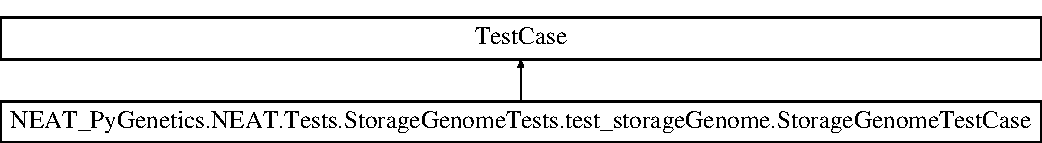
\includegraphics[height=1.927711cm]{class_n_e_a_t___py_genetics_1_1_n_e_a_t_1_1_tests_1_1_storage_genome_tests_1_1test__storage_genome_1_1_storage_genome_test_case}
\end{center}
\end{figure}
\subsection*{Public Member Functions}
\begin{DoxyCompactItemize}
\item 
def \hyperlink{class_n_e_a_t___py_genetics_1_1_n_e_a_t_1_1_tests_1_1_storage_genome_tests_1_1test__storage_genome_1_1_storage_genome_test_case_a27b58493e931470520a1e71e514009cb}{test\+\_\+eq} (self)
\item 
def {\bfseries test\+\_\+not\+Eq} (self)\hypertarget{class_n_e_a_t___py_genetics_1_1_n_e_a_t_1_1_tests_1_1_storage_genome_tests_1_1test__storage_genome_1_1_storage_genome_test_case_a01f81b00e989464c932df722135daf5c}{}\label{class_n_e_a_t___py_genetics_1_1_n_e_a_t_1_1_tests_1_1_storage_genome_tests_1_1test__storage_genome_1_1_storage_genome_test_case_a01f81b00e989464c932df722135daf5c}

\item 
def {\bfseries test\+\_\+copy\+Construct} (self)\hypertarget{class_n_e_a_t___py_genetics_1_1_n_e_a_t_1_1_tests_1_1_storage_genome_tests_1_1test__storage_genome_1_1_storage_genome_test_case_a4c670f9b3e78d2be50280880f1de23d5}{}\label{class_n_e_a_t___py_genetics_1_1_n_e_a_t_1_1_tests_1_1_storage_genome_tests_1_1test__storage_genome_1_1_storage_genome_test_case_a4c670f9b3e78d2be50280880f1de23d5}

\end{DoxyCompactItemize}


\subsection{Detailed Description}


Definition at line 9 of file test\+\_\+storage\+Genome.\+py.



\subsection{Member Function Documentation}
\index{N\+E\+A\+T\+\_\+\+Py\+Genetics\+::\+N\+E\+A\+T\+::\+Tests\+::\+Storage\+Genome\+Tests\+::test\+\_\+storage\+Genome\+::\+Storage\+Genome\+Test\+Case@{N\+E\+A\+T\+\_\+\+Py\+Genetics\+::\+N\+E\+A\+T\+::\+Tests\+::\+Storage\+Genome\+Tests\+::test\+\_\+storage\+Genome\+::\+Storage\+Genome\+Test\+Case}!test\+\_\+eq@{test\+\_\+eq}}
\index{test\+\_\+eq@{test\+\_\+eq}!N\+E\+A\+T\+\_\+\+Py\+Genetics\+::\+N\+E\+A\+T\+::\+Tests\+::\+Storage\+Genome\+Tests\+::test\+\_\+storage\+Genome\+::\+Storage\+Genome\+Test\+Case@{N\+E\+A\+T\+\_\+\+Py\+Genetics\+::\+N\+E\+A\+T\+::\+Tests\+::\+Storage\+Genome\+Tests\+::test\+\_\+storage\+Genome\+::\+Storage\+Genome\+Test\+Case}}
\subsubsection[{\texorpdfstring{test\+\_\+eq(self)}{test_eq(self)}}]{\setlength{\rightskip}{0pt plus 5cm}def N\+E\+A\+T\+\_\+\+Py\+Genetics.\+N\+E\+A\+T.\+Tests.\+Storage\+Genome\+Tests.\+test\+\_\+storage\+Genome.\+Storage\+Genome\+Test\+Case.\+test\+\_\+eq (
\begin{DoxyParamCaption}
\item[{}]{self}
\end{DoxyParamCaption}
)}\hypertarget{class_n_e_a_t___py_genetics_1_1_n_e_a_t_1_1_tests_1_1_storage_genome_tests_1_1test__storage_genome_1_1_storage_genome_test_case_a27b58493e931470520a1e71e514009cb}{}\label{class_n_e_a_t___py_genetics_1_1_n_e_a_t_1_1_tests_1_1_storage_genome_tests_1_1test__storage_genome_1_1_storage_genome_test_case_a27b58493e931470520a1e71e514009cb}
\begin{DoxyVerb}Tests, that the equality operator works.
:return:
\end{DoxyVerb}
 

Definition at line 10 of file test\+\_\+storage\+Genome.\+py.



The documentation for this class was generated from the following file\+:\begin{DoxyCompactItemize}
\item 
N\+E\+A\+T/\+Tests/\+Storage\+Genome\+Tests/test\+\_\+storage\+Genome.\+py\end{DoxyCompactItemize}

\hypertarget{class_n_e_a_t___py_genetics_1_1_n_e_a_t_1_1_tests_1_1_analyst_tests_1_1test__genome_selector_1_1test__genome_selector}{}\section{N\+E\+A\+T\+\_\+\+Py\+Genetics.\+N\+E\+A\+T.\+Tests.\+Analyst\+Tests.\+test\+\_\+genome\+Selector.\+test\+\_\+genome\+Selector Class Reference}
\label{class_n_e_a_t___py_genetics_1_1_n_e_a_t_1_1_tests_1_1_analyst_tests_1_1test__genome_selector_1_1test__genome_selector}\index{N\+E\+A\+T\+\_\+\+Py\+Genetics.\+N\+E\+A\+T.\+Tests.\+Analyst\+Tests.\+test\+\_\+genome\+Selector.\+test\+\_\+genome\+Selector@{N\+E\+A\+T\+\_\+\+Py\+Genetics.\+N\+E\+A\+T.\+Tests.\+Analyst\+Tests.\+test\+\_\+genome\+Selector.\+test\+\_\+genome\+Selector}}
Inheritance diagram for N\+E\+A\+T\+\_\+\+Py\+Genetics.\+N\+E\+A\+T.\+Tests.\+Analyst\+Tests.\+test\+\_\+genome\+Selector.\+test\+\_\+genome\+Selector\+:\begin{figure}[H]
\begin{center}
\leavevmode
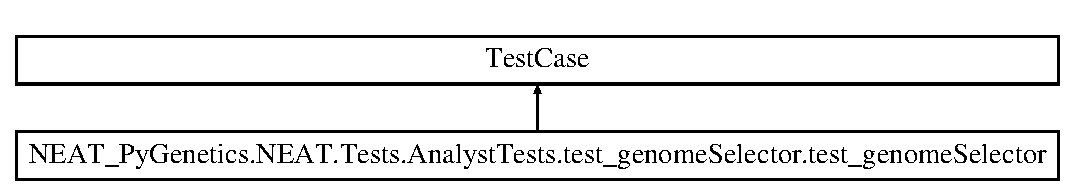
\includegraphics[height=2.000000cm]{class_n_e_a_t___py_genetics_1_1_n_e_a_t_1_1_tests_1_1_analyst_tests_1_1test__genome_selector_1_1test__genome_selector}
\end{center}
\end{figure}
\subsection*{Public Member Functions}
\begin{DoxyCompactItemize}
\item 
def {\bfseries set\+Up} (self)\hypertarget{class_n_e_a_t___py_genetics_1_1_n_e_a_t_1_1_tests_1_1_analyst_tests_1_1test__genome_selector_1_1test__genome_selector_a73634e74c61c8367095ed89b1a9ffa8d}{}\label{class_n_e_a_t___py_genetics_1_1_n_e_a_t_1_1_tests_1_1_analyst_tests_1_1test__genome_selector_1_1test__genome_selector_a73634e74c61c8367095ed89b1a9ffa8d}

\item 
def {\bfseries test\+\_\+get\+Genomes\+In\+Cluster} (self)\hypertarget{class_n_e_a_t___py_genetics_1_1_n_e_a_t_1_1_tests_1_1_analyst_tests_1_1test__genome_selector_1_1test__genome_selector_abf45d8dbc127efe9b7a89415b2f0b605}{}\label{class_n_e_a_t___py_genetics_1_1_n_e_a_t_1_1_tests_1_1_analyst_tests_1_1test__genome_selector_1_1test__genome_selector_abf45d8dbc127efe9b7a89415b2f0b605}

\item 
def {\bfseries test\+\_\+get\+Cluster\+Area\+Sorted\+By\+Fitness} (self)\hypertarget{class_n_e_a_t___py_genetics_1_1_n_e_a_t_1_1_tests_1_1_analyst_tests_1_1test__genome_selector_1_1test__genome_selector_a845cb361d31d78f62c573610a01c9c52}{}\label{class_n_e_a_t___py_genetics_1_1_n_e_a_t_1_1_tests_1_1_analyst_tests_1_1test__genome_selector_1_1test__genome_selector_a845cb361d31d78f62c573610a01c9c52}

\item 
def {\bfseries test\+\_\+select\+Genomes\+For\+Breeding\+\_\+and\+\_\+select\+Genomes\+For\+Mutation} (self)\hypertarget{class_n_e_a_t___py_genetics_1_1_n_e_a_t_1_1_tests_1_1_analyst_tests_1_1test__genome_selector_1_1test__genome_selector_abe868724b36a1423c915ca001bdfacb7}{}\label{class_n_e_a_t___py_genetics_1_1_n_e_a_t_1_1_tests_1_1_analyst_tests_1_1test__genome_selector_1_1test__genome_selector_abe868724b36a1423c915ca001bdfacb7}

\item 
def {\bfseries test\+\_\+select\+Cluster\+For\+Combination} (self)\hypertarget{class_n_e_a_t___py_genetics_1_1_n_e_a_t_1_1_tests_1_1_analyst_tests_1_1test__genome_selector_1_1test__genome_selector_a02f6228ac878117e968633e7d0652e37}{}\label{class_n_e_a_t___py_genetics_1_1_n_e_a_t_1_1_tests_1_1_analyst_tests_1_1test__genome_selector_1_1test__genome_selector_a02f6228ac878117e968633e7d0652e37}

\item 
def {\bfseries test\+\_\+select\+Cluster\+Combination} (self)\hypertarget{class_n_e_a_t___py_genetics_1_1_n_e_a_t_1_1_tests_1_1_analyst_tests_1_1test__genome_selector_1_1test__genome_selector_a1a32ff097226fd39d70886ef046293d4}{}\label{class_n_e_a_t___py_genetics_1_1_n_e_a_t_1_1_tests_1_1_analyst_tests_1_1test__genome_selector_1_1test__genome_selector_a1a32ff097226fd39d70886ef046293d4}

\item 
def \hyperlink{class_n_e_a_t___py_genetics_1_1_n_e_a_t_1_1_tests_1_1_analyst_tests_1_1test__genome_selector_1_1test__genome_selector_a5c10235f34e1e4e56e06ad1c17d787c5}{test\+\_\+select\+Genomes\+For\+Discarding} (self)
\end{DoxyCompactItemize}
\subsection*{Public Attributes}
\begin{DoxyCompactItemize}
\item 
{\bfseries mock\+\_\+genome\+\_\+repository}\hypertarget{class_n_e_a_t___py_genetics_1_1_n_e_a_t_1_1_tests_1_1_analyst_tests_1_1test__genome_selector_1_1test__genome_selector_af28f36e08d36b7693e8d181ee8143751}{}\label{class_n_e_a_t___py_genetics_1_1_n_e_a_t_1_1_tests_1_1_analyst_tests_1_1test__genome_selector_1_1test__genome_selector_af28f36e08d36b7693e8d181ee8143751}

\item 
{\bfseries mock\+\_\+cluster\+\_\+repository}\hypertarget{class_n_e_a_t___py_genetics_1_1_n_e_a_t_1_1_tests_1_1_analyst_tests_1_1test__genome_selector_1_1test__genome_selector_a54e3883498756f3e673b2eebc77890cb}{}\label{class_n_e_a_t___py_genetics_1_1_n_e_a_t_1_1_tests_1_1_analyst_tests_1_1test__genome_selector_1_1test__genome_selector_a54e3883498756f3e673b2eebc77890cb}

\item 
{\bfseries mock\+\_\+selection\+\_\+parameters}\hypertarget{class_n_e_a_t___py_genetics_1_1_n_e_a_t_1_1_tests_1_1_analyst_tests_1_1test__genome_selector_1_1test__genome_selector_ac77001932f6d9ab981a690257f7ff5d1}{}\label{class_n_e_a_t___py_genetics_1_1_n_e_a_t_1_1_tests_1_1_analyst_tests_1_1test__genome_selector_1_1test__genome_selector_ac77001932f6d9ab981a690257f7ff5d1}

\item 
{\bfseries genome\+\_\+selector}\hypertarget{class_n_e_a_t___py_genetics_1_1_n_e_a_t_1_1_tests_1_1_analyst_tests_1_1test__genome_selector_1_1test__genome_selector_a824c9616385543a8e9fe05a641932676}{}\label{class_n_e_a_t___py_genetics_1_1_n_e_a_t_1_1_tests_1_1_analyst_tests_1_1test__genome_selector_1_1test__genome_selector_a824c9616385543a8e9fe05a641932676}

\end{DoxyCompactItemize}


\subsection{Detailed Description}


Definition at line 9 of file test\+\_\+genome\+Selector.\+py.



\subsection{Member Function Documentation}
\index{N\+E\+A\+T\+\_\+\+Py\+Genetics\+::\+N\+E\+A\+T\+::\+Tests\+::\+Analyst\+Tests\+::test\+\_\+genome\+Selector\+::test\+\_\+genome\+Selector@{N\+E\+A\+T\+\_\+\+Py\+Genetics\+::\+N\+E\+A\+T\+::\+Tests\+::\+Analyst\+Tests\+::test\+\_\+genome\+Selector\+::test\+\_\+genome\+Selector}!test\+\_\+select\+Genomes\+For\+Discarding@{test\+\_\+select\+Genomes\+For\+Discarding}}
\index{test\+\_\+select\+Genomes\+For\+Discarding@{test\+\_\+select\+Genomes\+For\+Discarding}!N\+E\+A\+T\+\_\+\+Py\+Genetics\+::\+N\+E\+A\+T\+::\+Tests\+::\+Analyst\+Tests\+::test\+\_\+genome\+Selector\+::test\+\_\+genome\+Selector@{N\+E\+A\+T\+\_\+\+Py\+Genetics\+::\+N\+E\+A\+T\+::\+Tests\+::\+Analyst\+Tests\+::test\+\_\+genome\+Selector\+::test\+\_\+genome\+Selector}}
\subsubsection[{\texorpdfstring{test\+\_\+select\+Genomes\+For\+Discarding(self)}{test_selectGenomesForDiscarding(self)}}]{\setlength{\rightskip}{0pt plus 5cm}def N\+E\+A\+T\+\_\+\+Py\+Genetics.\+N\+E\+A\+T.\+Tests.\+Analyst\+Tests.\+test\+\_\+genome\+Selector.\+test\+\_\+genome\+Selector.\+test\+\_\+select\+Genomes\+For\+Discarding (
\begin{DoxyParamCaption}
\item[{}]{self}
\end{DoxyParamCaption}
)}\hypertarget{class_n_e_a_t___py_genetics_1_1_n_e_a_t_1_1_tests_1_1_analyst_tests_1_1test__genome_selector_1_1test__genome_selector_a5c10235f34e1e4e56e06ad1c17d787c5}{}\label{class_n_e_a_t___py_genetics_1_1_n_e_a_t_1_1_tests_1_1_analyst_tests_1_1test__genome_selector_1_1test__genome_selector_a5c10235f34e1e4e56e06ad1c17d787c5}
\begin{DoxyVerb}checks if 20% of worst cluster or genomes were selected
:return:
\end{DoxyVerb}
 

Definition at line 117 of file test\+\_\+genome\+Selector.\+py.



The documentation for this class was generated from the following file\+:\begin{DoxyCompactItemize}
\item 
N\+E\+A\+T/\+Tests/\+Analyst\+Tests/test\+\_\+genome\+Selector.\+py\end{DoxyCompactItemize}

\hypertarget{class_n_e_a_t___py_genetics_1_1_n_e_a_t_1_1_tests_1_1_analysis_genome_tests_1_1test__analysis_genome_1_1_test_analysis_genome}{}\section{N\+E\+A\+T\+\_\+\+Py\+Genetics.\+N\+E\+A\+T.\+Tests.\+Analysis\+Genome\+Tests.\+test\+\_\+analysis\+Genome.\+Test\+Analysis\+Genome Class Reference}
\label{class_n_e_a_t___py_genetics_1_1_n_e_a_t_1_1_tests_1_1_analysis_genome_tests_1_1test__analysis_genome_1_1_test_analysis_genome}\index{N\+E\+A\+T\+\_\+\+Py\+Genetics.\+N\+E\+A\+T.\+Tests.\+Analysis\+Genome\+Tests.\+test\+\_\+analysis\+Genome.\+Test\+Analysis\+Genome@{N\+E\+A\+T\+\_\+\+Py\+Genetics.\+N\+E\+A\+T.\+Tests.\+Analysis\+Genome\+Tests.\+test\+\_\+analysis\+Genome.\+Test\+Analysis\+Genome}}
Inheritance diagram for N\+E\+A\+T\+\_\+\+Py\+Genetics.\+N\+E\+A\+T.\+Tests.\+Analysis\+Genome\+Tests.\+test\+\_\+analysis\+Genome.\+Test\+Analysis\+Genome\+:\begin{figure}[H]
\begin{center}
\leavevmode
\includegraphics[height=1.985816cm]{class_n_e_a_t___py_genetics_1_1_n_e_a_t_1_1_tests_1_1_analysis_genome_tests_1_1test__analysis_genome_1_1_test_analysis_genome}
\end{center}
\end{figure}
\subsection*{Public Member Functions}
\begin{DoxyCompactItemize}
\item 
def {\bfseries set\+Up} (self)\hypertarget{class_n_e_a_t___py_genetics_1_1_n_e_a_t_1_1_tests_1_1_analysis_genome_tests_1_1test__analysis_genome_1_1_test_analysis_genome_a7eb8161235eddea20bc4c9663570cdac}{}\label{class_n_e_a_t___py_genetics_1_1_n_e_a_t_1_1_tests_1_1_analysis_genome_tests_1_1test__analysis_genome_1_1_test_analysis_genome_a7eb8161235eddea20bc4c9663570cdac}

\item 
def {\bfseries test\+\_\+\+\_\+add\+\_\+node} (self)\hypertarget{class_n_e_a_t___py_genetics_1_1_n_e_a_t_1_1_tests_1_1_analysis_genome_tests_1_1test__analysis_genome_1_1_test_analysis_genome_ac95b9d78e65bf92e330d9c44ed0ef3fc}{}\label{class_n_e_a_t___py_genetics_1_1_n_e_a_t_1_1_tests_1_1_analysis_genome_tests_1_1test__analysis_genome_1_1_test_analysis_genome_ac95b9d78e65bf92e330d9c44ed0ef3fc}

\item 
def {\bfseries test\+\_\+\+\_\+add\+\_\+edge} (self)\hypertarget{class_n_e_a_t___py_genetics_1_1_n_e_a_t_1_1_tests_1_1_analysis_genome_tests_1_1test__analysis_genome_1_1_test_analysis_genome_aaffe3eb85a13c66e0825223bae4ac78e}{}\label{class_n_e_a_t___py_genetics_1_1_n_e_a_t_1_1_tests_1_1_analysis_genome_tests_1_1test__analysis_genome_1_1_test_analysis_genome_aaffe3eb85a13c66e0825223bae4ac78e}

\item 
def {\bfseries test\+\_\+\+\_\+add\+\_\+edge\+\_\+without\+\_\+preadded\+\_\+nodes} (self)\hypertarget{class_n_e_a_t___py_genetics_1_1_n_e_a_t_1_1_tests_1_1_analysis_genome_tests_1_1test__analysis_genome_1_1_test_analysis_genome_a54eb6e20e337eeb03a7c31ee7339712f}{}\label{class_n_e_a_t___py_genetics_1_1_n_e_a_t_1_1_tests_1_1_analysis_genome_tests_1_1test__analysis_genome_1_1_test_analysis_genome_a54eb6e20e337eeb03a7c31ee7339712f}

\item 
def {\bfseries test\+\_\+\+\_\+add\+\_\+edge\+\_\+with\+\_\+preadded\+\_\+source\+\_\+node} (self)\hypertarget{class_n_e_a_t___py_genetics_1_1_n_e_a_t_1_1_tests_1_1_analysis_genome_tests_1_1test__analysis_genome_1_1_test_analysis_genome_a603ac3eb47164d8edb36630a92655adb}{}\label{class_n_e_a_t___py_genetics_1_1_n_e_a_t_1_1_tests_1_1_analysis_genome_tests_1_1test__analysis_genome_1_1_test_analysis_genome_a603ac3eb47164d8edb36630a92655adb}

\item 
def {\bfseries test\+\_\+init\+\_\+from\+\_\+storage\+\_\+structure} (self)\hypertarget{class_n_e_a_t___py_genetics_1_1_n_e_a_t_1_1_tests_1_1_analysis_genome_tests_1_1test__analysis_genome_1_1_test_analysis_genome_a24febdb8aa6bb2efff1f6dd77b4d4393}{}\label{class_n_e_a_t___py_genetics_1_1_n_e_a_t_1_1_tests_1_1_analysis_genome_tests_1_1test__analysis_genome_1_1_test_analysis_genome_a24febdb8aa6bb2efff1f6dd77b4d4393}

\item 
def {\bfseries test\+\_\+\+\_\+add\+\_\+input\+\_\+node} (self)\hypertarget{class_n_e_a_t___py_genetics_1_1_n_e_a_t_1_1_tests_1_1_analysis_genome_tests_1_1test__analysis_genome_1_1_test_analysis_genome_ad10dfce265aa3af67fb951add1fcdd34}{}\label{class_n_e_a_t___py_genetics_1_1_n_e_a_t_1_1_tests_1_1_analysis_genome_tests_1_1test__analysis_genome_1_1_test_analysis_genome_ad10dfce265aa3af67fb951add1fcdd34}

\item 
def {\bfseries test\+\_\+\+\_\+add\+\_\+output\+\_\+node} (self)\hypertarget{class_n_e_a_t___py_genetics_1_1_n_e_a_t_1_1_tests_1_1_analysis_genome_tests_1_1test__analysis_genome_1_1_test_analysis_genome_a59b12daf2e5e073af71aa97e0bb87009}{}\label{class_n_e_a_t___py_genetics_1_1_n_e_a_t_1_1_tests_1_1_analysis_genome_tests_1_1test__analysis_genome_1_1_test_analysis_genome_a59b12daf2e5e073af71aa97e0bb87009}

\end{DoxyCompactItemize}
\subsection*{Public Attributes}
\begin{DoxyCompactItemize}
\item 
{\bfseries mock\+\_\+gene\+\_\+repository}\hypertarget{class_n_e_a_t___py_genetics_1_1_n_e_a_t_1_1_tests_1_1_analysis_genome_tests_1_1test__analysis_genome_1_1_test_analysis_genome_a344a0b4458ba026a33e499da5ba58563}{}\label{class_n_e_a_t___py_genetics_1_1_n_e_a_t_1_1_tests_1_1_analysis_genome_tests_1_1test__analysis_genome_1_1_test_analysis_genome_a344a0b4458ba026a33e499da5ba58563}

\item 
{\bfseries storage\+\_\+genome}\hypertarget{class_n_e_a_t___py_genetics_1_1_n_e_a_t_1_1_tests_1_1_analysis_genome_tests_1_1test__analysis_genome_1_1_test_analysis_genome_a422f45a24e190778e830b08d527d2d66}{}\label{class_n_e_a_t___py_genetics_1_1_n_e_a_t_1_1_tests_1_1_analysis_genome_tests_1_1test__analysis_genome_1_1_test_analysis_genome_a422f45a24e190778e830b08d527d2d66}

\end{DoxyCompactItemize}


\subsection{Detailed Description}


Definition at line 8 of file test\+\_\+analysis\+Genome.\+py.



The documentation for this class was generated from the following file\+:\begin{DoxyCompactItemize}
\item 
N\+E\+A\+T/\+Tests/\+Analysis\+Genome\+Tests/test\+\_\+analysis\+Genome.\+py\end{DoxyCompactItemize}

\hypertarget{class_n_e_a_t___py_genetics_1_1_n_e_a_t_1_1_tests_1_1_analyst_tests_1_1test__analysis_result_1_1_test_analysis_result}{}\section{N\+E\+A\+T\+\_\+\+Py\+Genetics.\+N\+E\+A\+T.\+Tests.\+Analyst\+Tests.\+test\+\_\+analysis\+Result.\+Test\+Analysis\+Result Class Reference}
\label{class_n_e_a_t___py_genetics_1_1_n_e_a_t_1_1_tests_1_1_analyst_tests_1_1test__analysis_result_1_1_test_analysis_result}\index{N\+E\+A\+T\+\_\+\+Py\+Genetics.\+N\+E\+A\+T.\+Tests.\+Analyst\+Tests.\+test\+\_\+analysis\+Result.\+Test\+Analysis\+Result@{N\+E\+A\+T\+\_\+\+Py\+Genetics.\+N\+E\+A\+T.\+Tests.\+Analyst\+Tests.\+test\+\_\+analysis\+Result.\+Test\+Analysis\+Result}}
Inheritance diagram for N\+E\+A\+T\+\_\+\+Py\+Genetics.\+N\+E\+A\+T.\+Tests.\+Analyst\+Tests.\+test\+\_\+analysis\+Result.\+Test\+Analysis\+Result\+:\begin{figure}[H]
\begin{center}
\leavevmode
\includegraphics[height=2.000000cm]{class_n_e_a_t___py_genetics_1_1_n_e_a_t_1_1_tests_1_1_analyst_tests_1_1test__analysis_result_1_1_test_analysis_result}
\end{center}
\end{figure}
\subsection*{Public Member Functions}
\begin{DoxyCompactItemize}
\item 
def {\bfseries test\+\_\+equality\+\_\+operator} (self)\hypertarget{class_n_e_a_t___py_genetics_1_1_n_e_a_t_1_1_tests_1_1_analyst_tests_1_1test__analysis_result_1_1_test_analysis_result_ac7be3b7805195cdf50e994684a89e9a6}{}\label{class_n_e_a_t___py_genetics_1_1_n_e_a_t_1_1_tests_1_1_analyst_tests_1_1test__analysis_result_1_1_test_analysis_result_ac7be3b7805195cdf50e994684a89e9a6}

\item 
def {\bfseries test\+\_\+clear} (self)\hypertarget{class_n_e_a_t___py_genetics_1_1_n_e_a_t_1_1_tests_1_1_analyst_tests_1_1test__analysis_result_1_1_test_analysis_result_a936ce5fd67dd44d516a1cb5c9d3fe282}{}\label{class_n_e_a_t___py_genetics_1_1_n_e_a_t_1_1_tests_1_1_analyst_tests_1_1test__analysis_result_1_1_test_analysis_result_a936ce5fd67dd44d516a1cb5c9d3fe282}

\item 
def {\bfseries test\+\_\+cycle\+\_\+nodes} (self)\hypertarget{class_n_e_a_t___py_genetics_1_1_n_e_a_t_1_1_tests_1_1_analyst_tests_1_1test__analysis_result_1_1_test_analysis_result_a53fa99c33443988b4d9ec4bc99f6c252}{}\label{class_n_e_a_t___py_genetics_1_1_n_e_a_t_1_1_tests_1_1_analyst_tests_1_1test__analysis_result_1_1_test_analysis_result_a53fa99c33443988b4d9ec4bc99f6c252}

\item 
def {\bfseries test\+\_\+copy\+Constructor} (self)\hypertarget{class_n_e_a_t___py_genetics_1_1_n_e_a_t_1_1_tests_1_1_analyst_tests_1_1test__analysis_result_1_1_test_analysis_result_a8f560a4866c15837720dcf43ba95c725}{}\label{class_n_e_a_t___py_genetics_1_1_n_e_a_t_1_1_tests_1_1_analyst_tests_1_1test__analysis_result_1_1_test_analysis_result_a8f560a4866c15837720dcf43ba95c725}

\end{DoxyCompactItemize}


\subsection{Detailed Description}


Definition at line 5 of file test\+\_\+analysis\+Result.\+py.



The documentation for this class was generated from the following file\+:\begin{DoxyCompactItemize}
\item 
N\+E\+A\+T/\+Tests/\+Analyst\+Tests/test\+\_\+analysis\+Result.\+py\end{DoxyCompactItemize}

\hypertarget{class_n_e_a_t___py_genetics_1_1_n_e_a_t_1_1_tests_1_1_networking_tests_1_1_commands_tests_1_1tese8fe8884dc3553b68bdb031db05dd839}{}\section{N\+E\+A\+T\+\_\+\+Py\+Genetics.\+N\+E\+A\+T.\+Tests.\+Networking\+Tests.\+Commands\+Tests.\+test\+\_\+base\+Command.\+Test\+Base\+Command Class Reference}
\label{class_n_e_a_t___py_genetics_1_1_n_e_a_t_1_1_tests_1_1_networking_tests_1_1_commands_tests_1_1tese8fe8884dc3553b68bdb031db05dd839}\index{N\+E\+A\+T\+\_\+\+Py\+Genetics.\+N\+E\+A\+T.\+Tests.\+Networking\+Tests.\+Commands\+Tests.\+test\+\_\+base\+Command.\+Test\+Base\+Command@{N\+E\+A\+T\+\_\+\+Py\+Genetics.\+N\+E\+A\+T.\+Tests.\+Networking\+Tests.\+Commands\+Tests.\+test\+\_\+base\+Command.\+Test\+Base\+Command}}
Inheritance diagram for N\+E\+A\+T\+\_\+\+Py\+Genetics.\+N\+E\+A\+T.\+Tests.\+Networking\+Tests.\+Commands\+Tests.\+test\+\_\+base\+Command.\+Test\+Base\+Command\+:\begin{figure}[H]
\begin{center}
\leavevmode
\includegraphics[height=1.848185cm]{class_n_e_a_t___py_genetics_1_1_n_e_a_t_1_1_tests_1_1_networking_tests_1_1_commands_tests_1_1tese8fe8884dc3553b68bdb031db05dd839}
\end{center}
\end{figure}
\subsection*{Public Member Functions}
\begin{DoxyCompactItemize}
\item 
def {\bfseries set\+Up} (self)\hypertarget{class_n_e_a_t___py_genetics_1_1_n_e_a_t_1_1_tests_1_1_networking_tests_1_1_commands_tests_1_1tese8fe8884dc3553b68bdb031db05dd839_a9ea4f680b4693d49bf455f5f18ec3bff}{}\label{class_n_e_a_t___py_genetics_1_1_n_e_a_t_1_1_tests_1_1_networking_tests_1_1_commands_tests_1_1tese8fe8884dc3553b68bdb031db05dd839_a9ea4f680b4693d49bf455f5f18ec3bff}

\item 
def {\bfseries test\+\_\+from\+\_\+dict} (self)\hypertarget{class_n_e_a_t___py_genetics_1_1_n_e_a_t_1_1_tests_1_1_networking_tests_1_1_commands_tests_1_1tese8fe8884dc3553b68bdb031db05dd839_a7bbe5cd48c3e660972de4ef350395ef0}{}\label{class_n_e_a_t___py_genetics_1_1_n_e_a_t_1_1_tests_1_1_networking_tests_1_1_commands_tests_1_1tese8fe8884dc3553b68bdb031db05dd839_a7bbe5cd48c3e660972de4ef350395ef0}

\item 
def {\bfseries test\+\_\+as\+\_\+dict} (self)\hypertarget{class_n_e_a_t___py_genetics_1_1_n_e_a_t_1_1_tests_1_1_networking_tests_1_1_commands_tests_1_1tese8fe8884dc3553b68bdb031db05dd839_ad1ba157afd92a7ae452aad4680392eed}{}\label{class_n_e_a_t___py_genetics_1_1_n_e_a_t_1_1_tests_1_1_networking_tests_1_1_commands_tests_1_1tese8fe8884dc3553b68bdb031db05dd839_ad1ba157afd92a7ae452aad4680392eed}

\end{DoxyCompactItemize}
\subsection*{Public Attributes}
\begin{DoxyCompactItemize}
\item 
{\bfseries base\+\_\+command}\hypertarget{class_n_e_a_t___py_genetics_1_1_n_e_a_t_1_1_tests_1_1_networking_tests_1_1_commands_tests_1_1tese8fe8884dc3553b68bdb031db05dd839_ac704c0173d8ef7856a04cc83086bdfd6}{}\label{class_n_e_a_t___py_genetics_1_1_n_e_a_t_1_1_tests_1_1_networking_tests_1_1_commands_tests_1_1tese8fe8884dc3553b68bdb031db05dd839_ac704c0173d8ef7856a04cc83086bdfd6}

\item 
{\bfseries dictionary}\hypertarget{class_n_e_a_t___py_genetics_1_1_n_e_a_t_1_1_tests_1_1_networking_tests_1_1_commands_tests_1_1tese8fe8884dc3553b68bdb031db05dd839_a73e2d296a6b064d382f4a7261c499fb8}{}\label{class_n_e_a_t___py_genetics_1_1_n_e_a_t_1_1_tests_1_1_networking_tests_1_1_commands_tests_1_1tese8fe8884dc3553b68bdb031db05dd839_a73e2d296a6b064d382f4a7261c499fb8}

\end{DoxyCompactItemize}


\subsection{Detailed Description}


Definition at line 6 of file test\+\_\+base\+Command.\+py.



The documentation for this class was generated from the following file\+:\begin{DoxyCompactItemize}
\item 
N\+E\+A\+T/\+Tests/\+Networking\+Tests/\+Commands\+Tests/test\+\_\+base\+Command.\+py\end{DoxyCompactItemize}

\hypertarget{class_n_e_a_t___py_genetics_1_1_n_e_a_t_1_1_tests_1_1_breeder_tests_1_1test__breeder_1_1_test_breeder}{}\section{N\+E\+A\+T\+\_\+\+Py\+Genetics.\+N\+E\+A\+T.\+Tests.\+Breeder\+Tests.\+test\+\_\+breeder.\+Test\+Breeder Class Reference}
\label{class_n_e_a_t___py_genetics_1_1_n_e_a_t_1_1_tests_1_1_breeder_tests_1_1test__breeder_1_1_test_breeder}\index{N\+E\+A\+T\+\_\+\+Py\+Genetics.\+N\+E\+A\+T.\+Tests.\+Breeder\+Tests.\+test\+\_\+breeder.\+Test\+Breeder@{N\+E\+A\+T\+\_\+\+Py\+Genetics.\+N\+E\+A\+T.\+Tests.\+Breeder\+Tests.\+test\+\_\+breeder.\+Test\+Breeder}}
Inheritance diagram for N\+E\+A\+T\+\_\+\+Py\+Genetics.\+N\+E\+A\+T.\+Tests.\+Breeder\+Tests.\+test\+\_\+breeder.\+Test\+Breeder\+:\begin{figure}[H]
\begin{center}
\leavevmode
\includegraphics[height=2.000000cm]{class_n_e_a_t___py_genetics_1_1_n_e_a_t_1_1_tests_1_1_breeder_tests_1_1test__breeder_1_1_test_breeder}
\end{center}
\end{figure}
\subsection*{Public Member Functions}
\begin{DoxyCompactItemize}
\item 
def {\bfseries set\+Up} (self)\hypertarget{class_n_e_a_t___py_genetics_1_1_n_e_a_t_1_1_tests_1_1_breeder_tests_1_1test__breeder_1_1_test_breeder_a8967d8a2eed942a90b58d7b1201cb46c}{}\label{class_n_e_a_t___py_genetics_1_1_n_e_a_t_1_1_tests_1_1_breeder_tests_1_1test__breeder_1_1_test_breeder_a8967d8a2eed942a90b58d7b1201cb46c}

\item 
def {\bfseries test\+\_\+breed\+\_\+genomes} (self)\hypertarget{class_n_e_a_t___py_genetics_1_1_n_e_a_t_1_1_tests_1_1_breeder_tests_1_1test__breeder_1_1_test_breeder_a8595b48bc5d70d810bbe5aa38fc3175f}{}\label{class_n_e_a_t___py_genetics_1_1_n_e_a_t_1_1_tests_1_1_breeder_tests_1_1test__breeder_1_1_test_breeder_a8595b48bc5d70d810bbe5aa38fc3175f}

\end{DoxyCompactItemize}
\subsection*{Public Attributes}
\begin{DoxyCompactItemize}
\item 
{\bfseries breeder}\hypertarget{class_n_e_a_t___py_genetics_1_1_n_e_a_t_1_1_tests_1_1_breeder_tests_1_1test__breeder_1_1_test_breeder_abc027b8c1ce451c04c5eae1fe983c40b}{}\label{class_n_e_a_t___py_genetics_1_1_n_e_a_t_1_1_tests_1_1_breeder_tests_1_1test__breeder_1_1_test_breeder_abc027b8c1ce451c04c5eae1fe983c40b}

\end{DoxyCompactItemize}


\subsection{Detailed Description}


Definition at line 6 of file test\+\_\+breeder.\+py.



The documentation for this class was generated from the following file\+:\begin{DoxyCompactItemize}
\item 
N\+E\+A\+T/\+Tests/\+Breeder\+Tests/test\+\_\+breeder.\+py\end{DoxyCompactItemize}

\hypertarget{class_n_e_a_t___py_genetics_1_1_n_e_a_t_1_1_tests_1_1_repository_tests_1_1test__cluster_repository_1_1_test_cluster_repository}{}\section{N\+E\+A\+T\+\_\+\+Py\+Genetics.\+N\+E\+A\+T.\+Tests.\+Repository\+Tests.\+test\+\_\+cluster\+Repository.\+Test\+Cluster\+Repository Class Reference}
\label{class_n_e_a_t___py_genetics_1_1_n_e_a_t_1_1_tests_1_1_repository_tests_1_1test__cluster_repository_1_1_test_cluster_repository}\index{N\+E\+A\+T\+\_\+\+Py\+Genetics.\+N\+E\+A\+T.\+Tests.\+Repository\+Tests.\+test\+\_\+cluster\+Repository.\+Test\+Cluster\+Repository@{N\+E\+A\+T\+\_\+\+Py\+Genetics.\+N\+E\+A\+T.\+Tests.\+Repository\+Tests.\+test\+\_\+cluster\+Repository.\+Test\+Cluster\+Repository}}
Inheritance diagram for N\+E\+A\+T\+\_\+\+Py\+Genetics.\+N\+E\+A\+T.\+Tests.\+Repository\+Tests.\+test\+\_\+cluster\+Repository.\+Test\+Cluster\+Repository\+:\begin{figure}[H]
\begin{center}
\leavevmode
\includegraphics[height=2.000000cm]{class_n_e_a_t___py_genetics_1_1_n_e_a_t_1_1_tests_1_1_repository_tests_1_1test__cluster_repository_1_1_test_cluster_repository}
\end{center}
\end{figure}
\subsection*{Public Member Functions}
\begin{DoxyCompactItemize}
\item 
def {\bfseries set\+Up} (self)\hypertarget{class_n_e_a_t___py_genetics_1_1_n_e_a_t_1_1_tests_1_1_repository_tests_1_1test__cluster_repository_1_1_test_cluster_repository_ac796aabc9d2b5ede780a4a169c660730}{}\label{class_n_e_a_t___py_genetics_1_1_n_e_a_t_1_1_tests_1_1_repository_tests_1_1test__cluster_repository_1_1_test_cluster_repository_ac796aabc9d2b5ede780a4a169c660730}

\item 
def {\bfseries test\+\_\+get\+\_\+current\+\_\+clusters} (self)\hypertarget{class_n_e_a_t___py_genetics_1_1_n_e_a_t_1_1_tests_1_1_repository_tests_1_1test__cluster_repository_1_1_test_cluster_repository_a6994e2f71c1defcce3e4fbb22272d62a}{}\label{class_n_e_a_t___py_genetics_1_1_n_e_a_t_1_1_tests_1_1_repository_tests_1_1test__cluster_repository_1_1_test_cluster_repository_a6994e2f71c1defcce3e4fbb22272d62a}

\item 
def {\bfseries test\+\_\+add\+\_\+cluster\+\_\+with\+\_\+representative} (self)\hypertarget{class_n_e_a_t___py_genetics_1_1_n_e_a_t_1_1_tests_1_1_repository_tests_1_1test__cluster_repository_1_1_test_cluster_repository_a34e4a80f92b43e2436aefb6f506cf48f}{}\label{class_n_e_a_t___py_genetics_1_1_n_e_a_t_1_1_tests_1_1_repository_tests_1_1test__cluster_repository_1_1_test_cluster_repository_a34e4a80f92b43e2436aefb6f506cf48f}

\item 
def {\bfseries test\+\_\+archive\+\_\+cluster} (self)\hypertarget{class_n_e_a_t___py_genetics_1_1_n_e_a_t_1_1_tests_1_1_repository_tests_1_1test__cluster_repository_1_1_test_cluster_repository_a03c98f6f95e9085172a460da90718f15}{}\label{class_n_e_a_t___py_genetics_1_1_n_e_a_t_1_1_tests_1_1_repository_tests_1_1test__cluster_repository_1_1_test_cluster_repository_a03c98f6f95e9085172a460da90718f15}

\item 
def {\bfseries test\+\_\+get\+\_\+cluster\+\_\+by\+\_\+representative} (self)\hypertarget{class_n_e_a_t___py_genetics_1_1_n_e_a_t_1_1_tests_1_1_repository_tests_1_1test__cluster_repository_1_1_test_cluster_repository_aa46b728b0dd9bc39d491f1f93fad2205}{}\label{class_n_e_a_t___py_genetics_1_1_n_e_a_t_1_1_tests_1_1_repository_tests_1_1test__cluster_repository_1_1_test_cluster_repository_aa46b728b0dd9bc39d491f1f93fad2205}

\item 
def {\bfseries test\+\_\+get\+\_\+cluster\+\_\+count} (self)\hypertarget{class_n_e_a_t___py_genetics_1_1_n_e_a_t_1_1_tests_1_1_repository_tests_1_1test__cluster_repository_1_1_test_cluster_repository_acabc11488a7c53269dc9ed193b62a3e4}{}\label{class_n_e_a_t___py_genetics_1_1_n_e_a_t_1_1_tests_1_1_repository_tests_1_1test__cluster_repository_1_1_test_cluster_repository_acabc11488a7c53269dc9ed193b62a3e4}

\end{DoxyCompactItemize}
\subsection*{Public Attributes}
\begin{DoxyCompactItemize}
\item 
{\bfseries db}\hypertarget{class_n_e_a_t___py_genetics_1_1_n_e_a_t_1_1_tests_1_1_repository_tests_1_1test__cluster_repository_1_1_test_cluster_repository_a50cd224635a9b3ac6874c974ad6ffbc4}{}\label{class_n_e_a_t___py_genetics_1_1_n_e_a_t_1_1_tests_1_1_repository_tests_1_1test__cluster_repository_1_1_test_cluster_repository_a50cd224635a9b3ac6874c974ad6ffbc4}

\item 
{\bfseries cluster\+\_\+repository}\hypertarget{class_n_e_a_t___py_genetics_1_1_n_e_a_t_1_1_tests_1_1_repository_tests_1_1test__cluster_repository_1_1_test_cluster_repository_a8b29a81b6dbada0e6043c82570a684b7}{}\label{class_n_e_a_t___py_genetics_1_1_n_e_a_t_1_1_tests_1_1_repository_tests_1_1test__cluster_repository_1_1_test_cluster_repository_a8b29a81b6dbada0e6043c82570a684b7}

\end{DoxyCompactItemize}


\subsection{Detailed Description}


Definition at line 10 of file test\+\_\+cluster\+Repository.\+py.



The documentation for this class was generated from the following file\+:\begin{DoxyCompactItemize}
\item 
N\+E\+A\+T/\+Tests/\+Repository\+Tests/test\+\_\+cluster\+Repository.\+py\end{DoxyCompactItemize}

\hypertarget{class_n_e_a_t___py_genetics_1_1_n_e_a_t_1_1_tests_1_1_networking_tests_1_1_commands_tests_1_1tesf3907a6c11390aeeb9f3c9bdc4f3b133}{}\section{N\+E\+A\+T\+\_\+\+Py\+Genetics.\+N\+E\+A\+T.\+Tests.\+Networking\+Tests.\+Commands\+Tests.\+test\+\_\+command\+Transcoder.\+Test\+Command\+Transcoder Class Reference}
\label{class_n_e_a_t___py_genetics_1_1_n_e_a_t_1_1_tests_1_1_networking_tests_1_1_commands_tests_1_1tesf3907a6c11390aeeb9f3c9bdc4f3b133}\index{N\+E\+A\+T\+\_\+\+Py\+Genetics.\+N\+E\+A\+T.\+Tests.\+Networking\+Tests.\+Commands\+Tests.\+test\+\_\+command\+Transcoder.\+Test\+Command\+Transcoder@{N\+E\+A\+T\+\_\+\+Py\+Genetics.\+N\+E\+A\+T.\+Tests.\+Networking\+Tests.\+Commands\+Tests.\+test\+\_\+command\+Transcoder.\+Test\+Command\+Transcoder}}
Inheritance diagram for N\+E\+A\+T\+\_\+\+Py\+Genetics.\+N\+E\+A\+T.\+Tests.\+Networking\+Tests.\+Commands\+Tests.\+test\+\_\+command\+Transcoder.\+Test\+Command\+Transcoder\+:\begin{figure}[H]
\begin{center}
\leavevmode
\includegraphics[height=1.649485cm]{class_n_e_a_t___py_genetics_1_1_n_e_a_t_1_1_tests_1_1_networking_tests_1_1_commands_tests_1_1tesf3907a6c11390aeeb9f3c9bdc4f3b133}
\end{center}
\end{figure}
\subsection*{Public Member Functions}
\begin{DoxyCompactItemize}
\item 
def {\bfseries set\+Up} (self)\hypertarget{class_n_e_a_t___py_genetics_1_1_n_e_a_t_1_1_tests_1_1_networking_tests_1_1_commands_tests_1_1tesf3907a6c11390aeeb9f3c9bdc4f3b133_a2272af4f270fe071e01f4f958ae98f0c}{}\label{class_n_e_a_t___py_genetics_1_1_n_e_a_t_1_1_tests_1_1_networking_tests_1_1_commands_tests_1_1tesf3907a6c11390aeeb9f3c9bdc4f3b133_a2272af4f270fe071e01f4f958ae98f0c}

\item 
def {\bfseries test\+\_\+encode\+\_\+command} (self)\hypertarget{class_n_e_a_t___py_genetics_1_1_n_e_a_t_1_1_tests_1_1_networking_tests_1_1_commands_tests_1_1tesf3907a6c11390aeeb9f3c9bdc4f3b133_aa76781012dfd0b9e6c121d9d17c2167e}{}\label{class_n_e_a_t___py_genetics_1_1_n_e_a_t_1_1_tests_1_1_networking_tests_1_1_commands_tests_1_1tesf3907a6c11390aeeb9f3c9bdc4f3b133_aa76781012dfd0b9e6c121d9d17c2167e}

\item 
def {\bfseries test\+\_\+decode\+\_\+command} (self)\hypertarget{class_n_e_a_t___py_genetics_1_1_n_e_a_t_1_1_tests_1_1_networking_tests_1_1_commands_tests_1_1tesf3907a6c11390aeeb9f3c9bdc4f3b133_a64882d2ce98604b07d52cea3c2c71f7c}{}\label{class_n_e_a_t___py_genetics_1_1_n_e_a_t_1_1_tests_1_1_networking_tests_1_1_commands_tests_1_1tesf3907a6c11390aeeb9f3c9bdc4f3b133_a64882d2ce98604b07d52cea3c2c71f7c}

\end{DoxyCompactItemize}
\subsection*{Public Attributes}
\begin{DoxyCompactItemize}
\item 
{\bfseries base\+\_\+command}\hypertarget{class_n_e_a_t___py_genetics_1_1_n_e_a_t_1_1_tests_1_1_networking_tests_1_1_commands_tests_1_1tesf3907a6c11390aeeb9f3c9bdc4f3b133_ab37426eab44d5bf3cc1175ac7efac8a8}{}\label{class_n_e_a_t___py_genetics_1_1_n_e_a_t_1_1_tests_1_1_networking_tests_1_1_commands_tests_1_1tesf3907a6c11390aeeb9f3c9bdc4f3b133_ab37426eab44d5bf3cc1175ac7efac8a8}

\item 
{\bfseries command\+\_\+transcoder}\hypertarget{class_n_e_a_t___py_genetics_1_1_n_e_a_t_1_1_tests_1_1_networking_tests_1_1_commands_tests_1_1tesf3907a6c11390aeeb9f3c9bdc4f3b133_a28601736fc099584cd37ae3370fa8630}{}\label{class_n_e_a_t___py_genetics_1_1_n_e_a_t_1_1_tests_1_1_networking_tests_1_1_commands_tests_1_1tesf3907a6c11390aeeb9f3c9bdc4f3b133_a28601736fc099584cd37ae3370fa8630}

\end{DoxyCompactItemize}


\subsection{Detailed Description}


Definition at line 7 of file test\+\_\+command\+Transcoder.\+py.



The documentation for this class was generated from the following file\+:\begin{DoxyCompactItemize}
\item 
N\+E\+A\+T/\+Tests/\+Networking\+Tests/\+Commands\+Tests/test\+\_\+command\+Transcoder.\+py\end{DoxyCompactItemize}

\hypertarget{class_n_e_a_t___py_genetics_1_1_n_e_a_t_1_1_tests_1_1_decisions_1_1test__decision_maker_1_1_test_decision_maker}{}\section{N\+E\+A\+T\+\_\+\+Py\+Genetics.\+N\+E\+A\+T.\+Tests.\+Decisions.\+test\+\_\+decision\+Maker.\+Test\+Decision\+Maker Class Reference}
\label{class_n_e_a_t___py_genetics_1_1_n_e_a_t_1_1_tests_1_1_decisions_1_1test__decision_maker_1_1_test_decision_maker}\index{N\+E\+A\+T\+\_\+\+Py\+Genetics.\+N\+E\+A\+T.\+Tests.\+Decisions.\+test\+\_\+decision\+Maker.\+Test\+Decision\+Maker@{N\+E\+A\+T\+\_\+\+Py\+Genetics.\+N\+E\+A\+T.\+Tests.\+Decisions.\+test\+\_\+decision\+Maker.\+Test\+Decision\+Maker}}
Inheritance diagram for N\+E\+A\+T\+\_\+\+Py\+Genetics.\+N\+E\+A\+T.\+Tests.\+Decisions.\+test\+\_\+decision\+Maker.\+Test\+Decision\+Maker\+:\begin{figure}[H]
\begin{center}
\leavevmode
\includegraphics[height=2.000000cm]{class_n_e_a_t___py_genetics_1_1_n_e_a_t_1_1_tests_1_1_decisions_1_1test__decision_maker_1_1_test_decision_maker}
\end{center}
\end{figure}
\subsection*{Public Member Functions}
\begin{DoxyCompactItemize}
\item 
def {\bfseries set\+Up} (self)\hypertarget{class_n_e_a_t___py_genetics_1_1_n_e_a_t_1_1_tests_1_1_decisions_1_1test__decision_maker_1_1_test_decision_maker_ae743e3cceb0734c4d2004ce832e19b37}{}\label{class_n_e_a_t___py_genetics_1_1_n_e_a_t_1_1_tests_1_1_decisions_1_1test__decision_maker_1_1_test_decision_maker_ae743e3cceb0734c4d2004ce832e19b37}

\item 
def {\bfseries test\+\_\+advance\+\_\+time} (self)\hypertarget{class_n_e_a_t___py_genetics_1_1_n_e_a_t_1_1_tests_1_1_decisions_1_1test__decision_maker_1_1_test_decision_maker_a430c0500eb51d4eb2a829deecc92190b}{}\label{class_n_e_a_t___py_genetics_1_1_n_e_a_t_1_1_tests_1_1_decisions_1_1test__decision_maker_1_1_test_decision_maker_a430c0500eb51d4eb2a829deecc92190b}

\item 
def {\bfseries test\+\_\+reset\+\_\+time} (self)\hypertarget{class_n_e_a_t___py_genetics_1_1_n_e_a_t_1_1_tests_1_1_decisions_1_1test__decision_maker_1_1_test_decision_maker_a10ef93cd00575a620e36c175774a8992}{}\label{class_n_e_a_t___py_genetics_1_1_n_e_a_t_1_1_tests_1_1_decisions_1_1test__decision_maker_1_1_test_decision_maker_a10ef93cd00575a620e36c175774a8992}

\item 
def {\bfseries test\+\_\+mutation\+\_\+percentage} (self)\hypertarget{class_n_e_a_t___py_genetics_1_1_n_e_a_t_1_1_tests_1_1_decisions_1_1test__decision_maker_1_1_test_decision_maker_a67242115e3c1ebb7136d09e1918b6454}{}\label{class_n_e_a_t___py_genetics_1_1_n_e_a_t_1_1_tests_1_1_decisions_1_1test__decision_maker_1_1_test_decision_maker_a67242115e3c1ebb7136d09e1918b6454}

\item 
def {\bfseries test\+\_\+inter\+\_\+cluster\+\_\+breeding\+\_\+time} (self)\hypertarget{class_n_e_a_t___py_genetics_1_1_n_e_a_t_1_1_tests_1_1_decisions_1_1test__decision_maker_1_1_test_decision_maker_ab1fceb1b0d9a33d3ede5baad0cf054e0}{}\label{class_n_e_a_t___py_genetics_1_1_n_e_a_t_1_1_tests_1_1_decisions_1_1test__decision_maker_1_1_test_decision_maker_ab1fceb1b0d9a33d3ede5baad0cf054e0}

\item 
def {\bfseries test\+\_\+\+\_\+cutoff\+\_\+function} (self)\hypertarget{class_n_e_a_t___py_genetics_1_1_n_e_a_t_1_1_tests_1_1_decisions_1_1test__decision_maker_1_1_test_decision_maker_a80e9b89bcdb7044751b2cfb1469e40fd}{}\label{class_n_e_a_t___py_genetics_1_1_n_e_a_t_1_1_tests_1_1_decisions_1_1test__decision_maker_1_1_test_decision_maker_a80e9b89bcdb7044751b2cfb1469e40fd}

\end{DoxyCompactItemize}
\subsection*{Public Attributes}
\begin{DoxyCompactItemize}
\item 
{\bfseries selection\+\_\+parameter}\hypertarget{class_n_e_a_t___py_genetics_1_1_n_e_a_t_1_1_tests_1_1_decisions_1_1test__decision_maker_1_1_test_decision_maker_a48bf19a9ef756a110e01193d8a9e893e}{}\label{class_n_e_a_t___py_genetics_1_1_n_e_a_t_1_1_tests_1_1_decisions_1_1test__decision_maker_1_1_test_decision_maker_a48bf19a9ef756a110e01193d8a9e893e}

\item 
{\bfseries decision\+\_\+maker}\hypertarget{class_n_e_a_t___py_genetics_1_1_n_e_a_t_1_1_tests_1_1_decisions_1_1test__decision_maker_1_1_test_decision_maker_a5508e5f40a239a5ea7d682d7473a0da0}{}\label{class_n_e_a_t___py_genetics_1_1_n_e_a_t_1_1_tests_1_1_decisions_1_1test__decision_maker_1_1_test_decision_maker_a5508e5f40a239a5ea7d682d7473a0da0}

\end{DoxyCompactItemize}


\subsection{Detailed Description}


Definition at line 7 of file test\+\_\+decision\+Maker.\+py.



The documentation for this class was generated from the following file\+:\begin{DoxyCompactItemize}
\item 
N\+E\+A\+T/\+Tests/\+Decisions/test\+\_\+decision\+Maker.\+py\end{DoxyCompactItemize}

\hypertarget{class_n_e_a_t___py_genetics_1_1_n_e_a_t_1_1_tests_1_1_repository_tests_1_1test__gene_repository_1_1_test_gene_repository}{}\section{N\+E\+A\+T\+\_\+\+Py\+Genetics.\+N\+E\+A\+T.\+Tests.\+Repository\+Tests.\+test\+\_\+gene\+Repository.\+Test\+Gene\+Repository Class Reference}
\label{class_n_e_a_t___py_genetics_1_1_n_e_a_t_1_1_tests_1_1_repository_tests_1_1test__gene_repository_1_1_test_gene_repository}\index{N\+E\+A\+T\+\_\+\+Py\+Genetics.\+N\+E\+A\+T.\+Tests.\+Repository\+Tests.\+test\+\_\+gene\+Repository.\+Test\+Gene\+Repository@{N\+E\+A\+T\+\_\+\+Py\+Genetics.\+N\+E\+A\+T.\+Tests.\+Repository\+Tests.\+test\+\_\+gene\+Repository.\+Test\+Gene\+Repository}}
Inheritance diagram for N\+E\+A\+T\+\_\+\+Py\+Genetics.\+N\+E\+A\+T.\+Tests.\+Repository\+Tests.\+test\+\_\+gene\+Repository.\+Test\+Gene\+Repository\+:\begin{figure}[H]
\begin{center}
\leavevmode
\includegraphics[height=2.000000cm]{class_n_e_a_t___py_genetics_1_1_n_e_a_t_1_1_tests_1_1_repository_tests_1_1test__gene_repository_1_1_test_gene_repository}
\end{center}
\end{figure}
\subsection*{Public Member Functions}
\begin{DoxyCompactItemize}
\item 
def {\bfseries test\+\_\+get\+\_\+gene\+\_\+id\+\_\+for\+\_\+endpoints} (self)\hypertarget{class_n_e_a_t___py_genetics_1_1_n_e_a_t_1_1_tests_1_1_repository_tests_1_1test__gene_repository_1_1_test_gene_repository_a9688b85e7f9a1eade7514bee5e4976e1}{}\label{class_n_e_a_t___py_genetics_1_1_n_e_a_t_1_1_tests_1_1_repository_tests_1_1test__gene_repository_1_1_test_gene_repository_a9688b85e7f9a1eade7514bee5e4976e1}

\item 
def {\bfseries test\+\_\+find\+\_\+connecting\+\_\+nodes} (self)\hypertarget{class_n_e_a_t___py_genetics_1_1_n_e_a_t_1_1_tests_1_1_repository_tests_1_1test__gene_repository_1_1_test_gene_repository_a1e243ceab606dbf34e054672cb2695b3}{}\label{class_n_e_a_t___py_genetics_1_1_n_e_a_t_1_1_tests_1_1_repository_tests_1_1test__gene_repository_1_1_test_gene_repository_a1e243ceab606dbf34e054672cb2695b3}

\item 
def {\bfseries test\+\_\+get\+\_\+next\+\_\+node\+\_\+label} (self)\hypertarget{class_n_e_a_t___py_genetics_1_1_n_e_a_t_1_1_tests_1_1_repository_tests_1_1test__gene_repository_1_1_test_gene_repository_af1ecb2f51fa36fee4c9dc2b8e9b49348}{}\label{class_n_e_a_t___py_genetics_1_1_n_e_a_t_1_1_tests_1_1_repository_tests_1_1test__gene_repository_1_1_test_gene_repository_af1ecb2f51fa36fee4c9dc2b8e9b49348}

\item 
def {\bfseries test\+\_\+get\+\_\+node\+\_\+labels\+\_\+by\+\_\+gene\+\_\+id} (self)\hypertarget{class_n_e_a_t___py_genetics_1_1_n_e_a_t_1_1_tests_1_1_repository_tests_1_1test__gene_repository_1_1_test_gene_repository_a8928178404a7f810e00610192a8fd368}{}\label{class_n_e_a_t___py_genetics_1_1_n_e_a_t_1_1_tests_1_1_repository_tests_1_1test__gene_repository_1_1_test_gene_repository_a8928178404a7f810e00610192a8fd368}

\end{DoxyCompactItemize}


\subsection{Detailed Description}


Definition at line 6 of file test\+\_\+gene\+Repository.\+py.



The documentation for this class was generated from the following file\+:\begin{DoxyCompactItemize}
\item 
N\+E\+A\+T/\+Tests/\+Repository\+Tests/test\+\_\+gene\+Repository.\+py\end{DoxyCompactItemize}

\hypertarget{class_n_e_a_t___py_genetics_1_1_n_e_a_t_1_1_tests_1_1_analyst_tests_1_1test__genome_analyst_1_1_test_genome_analyst}{}\section{N\+E\+A\+T\+\_\+\+Py\+Genetics.\+N\+E\+A\+T.\+Tests.\+Analyst\+Tests.\+test\+\_\+genome\+Analyst.\+Test\+Genome\+Analyst Class Reference}
\label{class_n_e_a_t___py_genetics_1_1_n_e_a_t_1_1_tests_1_1_analyst_tests_1_1test__genome_analyst_1_1_test_genome_analyst}\index{N\+E\+A\+T\+\_\+\+Py\+Genetics.\+N\+E\+A\+T.\+Tests.\+Analyst\+Tests.\+test\+\_\+genome\+Analyst.\+Test\+Genome\+Analyst@{N\+E\+A\+T\+\_\+\+Py\+Genetics.\+N\+E\+A\+T.\+Tests.\+Analyst\+Tests.\+test\+\_\+genome\+Analyst.\+Test\+Genome\+Analyst}}
Inheritance diagram for N\+E\+A\+T\+\_\+\+Py\+Genetics.\+N\+E\+A\+T.\+Tests.\+Analyst\+Tests.\+test\+\_\+genome\+Analyst.\+Test\+Genome\+Analyst\+:\begin{figure}[H]
\begin{center}
\leavevmode
\includegraphics[height=2.000000cm]{class_n_e_a_t___py_genetics_1_1_n_e_a_t_1_1_tests_1_1_analyst_tests_1_1test__genome_analyst_1_1_test_genome_analyst}
\end{center}
\end{figure}
\subsection*{Public Member Functions}
\begin{DoxyCompactItemize}
\item 
def {\bfseries test\+\_\+analysis\+By\+Example} (self)\hypertarget{class_n_e_a_t___py_genetics_1_1_n_e_a_t_1_1_tests_1_1_analyst_tests_1_1test__genome_analyst_1_1_test_genome_analyst_a53539d6400718b534692e71255228de4}{}\label{class_n_e_a_t___py_genetics_1_1_n_e_a_t_1_1_tests_1_1_analyst_tests_1_1test__genome_analyst_1_1_test_genome_analyst_a53539d6400718b534692e71255228de4}

\end{DoxyCompactItemize}


\subsection{Detailed Description}


Definition at line 7 of file test\+\_\+genome\+Analyst.\+py.



The documentation for this class was generated from the following file\+:\begin{DoxyCompactItemize}
\item 
N\+E\+A\+T/\+Tests/\+Analyst\+Tests/test\+\_\+genome\+Analyst.\+py\end{DoxyCompactItemize}

\hypertarget{class_n_e_a_t___py_genetics_1_1_n_e_a_t_1_1_tests_1_1_genome_clusterer_tests_1_1test__genome_clu8e5a0289e00c807a0d74c340ea42f50e}{}\section{N\+E\+A\+T\+\_\+\+Py\+Genetics.\+N\+E\+A\+T.\+Tests.\+Genome\+Clusterer\+Tests.\+test\+\_\+genome\+Clusterer.\+Test\+Genome\+Clusterer Class Reference}
\label{class_n_e_a_t___py_genetics_1_1_n_e_a_t_1_1_tests_1_1_genome_clusterer_tests_1_1test__genome_clu8e5a0289e00c807a0d74c340ea42f50e}\index{N\+E\+A\+T\+\_\+\+Py\+Genetics.\+N\+E\+A\+T.\+Tests.\+Genome\+Clusterer\+Tests.\+test\+\_\+genome\+Clusterer.\+Test\+Genome\+Clusterer@{N\+E\+A\+T\+\_\+\+Py\+Genetics.\+N\+E\+A\+T.\+Tests.\+Genome\+Clusterer\+Tests.\+test\+\_\+genome\+Clusterer.\+Test\+Genome\+Clusterer}}
Inheritance diagram for N\+E\+A\+T\+\_\+\+Py\+Genetics.\+N\+E\+A\+T.\+Tests.\+Genome\+Clusterer\+Tests.\+test\+\_\+genome\+Clusterer.\+Test\+Genome\+Clusterer\+:\begin{figure}[H]
\begin{center}
\leavevmode
\includegraphics[height=1.944445cm]{class_n_e_a_t___py_genetics_1_1_n_e_a_t_1_1_tests_1_1_genome_clusterer_tests_1_1test__genome_clu8e5a0289e00c807a0d74c340ea42f50e}
\end{center}
\end{figure}
\subsection*{Public Member Functions}
\begin{DoxyCompactItemize}
\item 
def {\bfseries set\+Up} (self)\hypertarget{class_n_e_a_t___py_genetics_1_1_n_e_a_t_1_1_tests_1_1_genome_clusterer_tests_1_1test__genome_clu8e5a0289e00c807a0d74c340ea42f50e_ad0bdd164ebb6347c8beb4ddf7742fb52}{}\label{class_n_e_a_t___py_genetics_1_1_n_e_a_t_1_1_tests_1_1_genome_clusterer_tests_1_1test__genome_clu8e5a0289e00c807a0d74c340ea42f50e_ad0bdd164ebb6347c8beb4ddf7742fb52}

\item 
def {\bfseries test\+\_\+cluster\+\_\+genome\+\_\+no\+\_\+clusters} (self)\hypertarget{class_n_e_a_t___py_genetics_1_1_n_e_a_t_1_1_tests_1_1_genome_clusterer_tests_1_1test__genome_clu8e5a0289e00c807a0d74c340ea42f50e_a66e6a11e2e6d41bc5a8b276560029e96}{}\label{class_n_e_a_t___py_genetics_1_1_n_e_a_t_1_1_tests_1_1_genome_clusterer_tests_1_1test__genome_clu8e5a0289e00c807a0d74c340ea42f50e_a66e6a11e2e6d41bc5a8b276560029e96}

\item 
def {\bfseries test\+\_\+cluster\+\_\+genome\+\_\+no\+\_\+delta\+\_\+less} (self)\hypertarget{class_n_e_a_t___py_genetics_1_1_n_e_a_t_1_1_tests_1_1_genome_clusterer_tests_1_1test__genome_clu8e5a0289e00c807a0d74c340ea42f50e_ab619a0c345abbaf2ff03e990c514d193}{}\label{class_n_e_a_t___py_genetics_1_1_n_e_a_t_1_1_tests_1_1_genome_clusterer_tests_1_1test__genome_clu8e5a0289e00c807a0d74c340ea42f50e_ab619a0c345abbaf2ff03e990c514d193}

\item 
def {\bfseries test\+\_\+cluster\+\_\+genome\+\_\+with\+\_\+delta\+\_\+less} (self)\hypertarget{class_n_e_a_t___py_genetics_1_1_n_e_a_t_1_1_tests_1_1_genome_clusterer_tests_1_1test__genome_clu8e5a0289e00c807a0d74c340ea42f50e_a75b6137cf256927638ce38b23d0b8d0d}{}\label{class_n_e_a_t___py_genetics_1_1_n_e_a_t_1_1_tests_1_1_genome_clusterer_tests_1_1test__genome_clu8e5a0289e00c807a0d74c340ea42f50e_a75b6137cf256927638ce38b23d0b8d0d}

\item 
def {\bfseries test\+\_\+calculate\+\_\+delta} (self)\hypertarget{class_n_e_a_t___py_genetics_1_1_n_e_a_t_1_1_tests_1_1_genome_clusterer_tests_1_1test__genome_clu8e5a0289e00c807a0d74c340ea42f50e_a677e1ee47c1688bfab9c2c183921aa1c}{}\label{class_n_e_a_t___py_genetics_1_1_n_e_a_t_1_1_tests_1_1_genome_clusterer_tests_1_1test__genome_clu8e5a0289e00c807a0d74c340ea42f50e_a677e1ee47c1688bfab9c2c183921aa1c}

\item 
def {\bfseries test\+\_\+calculate\+\_\+disjoint\+\_\+excess\+\_\+count} (self)\hypertarget{class_n_e_a_t___py_genetics_1_1_n_e_a_t_1_1_tests_1_1_genome_clusterer_tests_1_1test__genome_clu8e5a0289e00c807a0d74c340ea42f50e_a31a46433f70bd1b7a4b3f480899c612f}{}\label{class_n_e_a_t___py_genetics_1_1_n_e_a_t_1_1_tests_1_1_genome_clusterer_tests_1_1test__genome_clu8e5a0289e00c807a0d74c340ea42f50e_a31a46433f70bd1b7a4b3f480899c612f}

\item 
def {\bfseries test\+\_\+calculate\+\_\+w\+\_\+bar} (self)\hypertarget{class_n_e_a_t___py_genetics_1_1_n_e_a_t_1_1_tests_1_1_genome_clusterer_tests_1_1test__genome_clu8e5a0289e00c807a0d74c340ea42f50e_ac3c3bbcc8ab434021544730fdaff33fb}{}\label{class_n_e_a_t___py_genetics_1_1_n_e_a_t_1_1_tests_1_1_genome_clusterer_tests_1_1test__genome_clu8e5a0289e00c807a0d74c340ea42f50e_ac3c3bbcc8ab434021544730fdaff33fb}

\item 
def {\bfseries test\+\_\+calculate\+\_\+cluster\+\_\+fitness} (self)\hypertarget{class_n_e_a_t___py_genetics_1_1_n_e_a_t_1_1_tests_1_1_genome_clusterer_tests_1_1test__genome_clu8e5a0289e00c807a0d74c340ea42f50e_a825bce2fcf584d1947fcfcb555357fb1}{}\label{class_n_e_a_t___py_genetics_1_1_n_e_a_t_1_1_tests_1_1_genome_clusterer_tests_1_1test__genome_clu8e5a0289e00c807a0d74c340ea42f50e_a825bce2fcf584d1947fcfcb555357fb1}

\item 
def {\bfseries test\+\_\+calculate\+\_\+cluster\+\_\+offspring\+\_\+values} (self)\hypertarget{class_n_e_a_t___py_genetics_1_1_n_e_a_t_1_1_tests_1_1_genome_clusterer_tests_1_1test__genome_clu8e5a0289e00c807a0d74c340ea42f50e_a750f3d1f911e2046b2f333c2d8a80f20}{}\label{class_n_e_a_t___py_genetics_1_1_n_e_a_t_1_1_tests_1_1_genome_clusterer_tests_1_1test__genome_clu8e5a0289e00c807a0d74c340ea42f50e_a750f3d1f911e2046b2f333c2d8a80f20}

\end{DoxyCompactItemize}
\subsection*{Public Attributes}
\begin{DoxyCompactItemize}
\item 
{\bfseries clustering\+\_\+parameters}\hypertarget{class_n_e_a_t___py_genetics_1_1_n_e_a_t_1_1_tests_1_1_genome_clusterer_tests_1_1test__genome_clu8e5a0289e00c807a0d74c340ea42f50e_a9cc349e3e78e1616840e36bcfd3a6834}{}\label{class_n_e_a_t___py_genetics_1_1_n_e_a_t_1_1_tests_1_1_genome_clusterer_tests_1_1test__genome_clu8e5a0289e00c807a0d74c340ea42f50e_a9cc349e3e78e1616840e36bcfd3a6834}

\item 
{\bfseries db\+\_\+connector}\hypertarget{class_n_e_a_t___py_genetics_1_1_n_e_a_t_1_1_tests_1_1_genome_clusterer_tests_1_1test__genome_clu8e5a0289e00c807a0d74c340ea42f50e_aa5acaa2c17a115c32c5317a067be0016}{}\label{class_n_e_a_t___py_genetics_1_1_n_e_a_t_1_1_tests_1_1_genome_clusterer_tests_1_1test__genome_clu8e5a0289e00c807a0d74c340ea42f50e_aa5acaa2c17a115c32c5317a067be0016}

\item 
{\bfseries mock\+\_\+genome\+\_\+repository}\hypertarget{class_n_e_a_t___py_genetics_1_1_n_e_a_t_1_1_tests_1_1_genome_clusterer_tests_1_1test__genome_clu8e5a0289e00c807a0d74c340ea42f50e_a1abfe40b10ff6d4cd6a58f4fca6c76b8}{}\label{class_n_e_a_t___py_genetics_1_1_n_e_a_t_1_1_tests_1_1_genome_clusterer_tests_1_1test__genome_clu8e5a0289e00c807a0d74c340ea42f50e_a1abfe40b10ff6d4cd6a58f4fca6c76b8}

\item 
{\bfseries mock\+\_\+cluster\+\_\+repository}\hypertarget{class_n_e_a_t___py_genetics_1_1_n_e_a_t_1_1_tests_1_1_genome_clusterer_tests_1_1test__genome_clu8e5a0289e00c807a0d74c340ea42f50e_a78d0e64bf2b3100d5d291f433c7020eb}{}\label{class_n_e_a_t___py_genetics_1_1_n_e_a_t_1_1_tests_1_1_genome_clusterer_tests_1_1test__genome_clu8e5a0289e00c807a0d74c340ea42f50e_a78d0e64bf2b3100d5d291f433c7020eb}

\item 
{\bfseries genome\+\_\+clusterer}\hypertarget{class_n_e_a_t___py_genetics_1_1_n_e_a_t_1_1_tests_1_1_genome_clusterer_tests_1_1test__genome_clu8e5a0289e00c807a0d74c340ea42f50e_a73efd20ba6c48aeab0c9fe41a444c334}{}\label{class_n_e_a_t___py_genetics_1_1_n_e_a_t_1_1_tests_1_1_genome_clusterer_tests_1_1test__genome_clu8e5a0289e00c807a0d74c340ea42f50e_a73efd20ba6c48aeab0c9fe41a444c334}

\end{DoxyCompactItemize}


\subsection{Detailed Description}


Definition at line 15 of file test\+\_\+genome\+Clusterer.\+py.



The documentation for this class was generated from the following file\+:\begin{DoxyCompactItemize}
\item 
N\+E\+A\+T/\+Tests/\+Genome\+Clusterer\+Tests/test\+\_\+genome\+Clusterer.\+py\end{DoxyCompactItemize}

\hypertarget{class_n_e_a_t___py_genetics_1_1_n_e_a_t_1_1_tests_1_1_repository_tests_1_1test__genome_repository_1_1_test_genome_repository}{}\section{N\+E\+A\+T\+\_\+\+Py\+Genetics.\+N\+E\+A\+T.\+Tests.\+Repository\+Tests.\+test\+\_\+genome\+Repository.\+Test\+Genome\+Repository Class Reference}
\label{class_n_e_a_t___py_genetics_1_1_n_e_a_t_1_1_tests_1_1_repository_tests_1_1test__genome_repository_1_1_test_genome_repository}\index{N\+E\+A\+T\+\_\+\+Py\+Genetics.\+N\+E\+A\+T.\+Tests.\+Repository\+Tests.\+test\+\_\+genome\+Repository.\+Test\+Genome\+Repository@{N\+E\+A\+T\+\_\+\+Py\+Genetics.\+N\+E\+A\+T.\+Tests.\+Repository\+Tests.\+test\+\_\+genome\+Repository.\+Test\+Genome\+Repository}}
Inheritance diagram for N\+E\+A\+T\+\_\+\+Py\+Genetics.\+N\+E\+A\+T.\+Tests.\+Repository\+Tests.\+test\+\_\+genome\+Repository.\+Test\+Genome\+Repository\+:\begin{figure}[H]
\begin{center}
\leavevmode
\includegraphics[height=2.000000cm]{class_n_e_a_t___py_genetics_1_1_n_e_a_t_1_1_tests_1_1_repository_tests_1_1test__genome_repository_1_1_test_genome_repository}
\end{center}
\end{figure}
\subsection*{Public Member Functions}
\begin{DoxyCompactItemize}
\item 
def {\bfseries set\+Up} (self)\hypertarget{class_n_e_a_t___py_genetics_1_1_n_e_a_t_1_1_tests_1_1_repository_tests_1_1test__genome_repository_1_1_test_genome_repository_ae2b7ccc2f82109fc883a638a5d2f20e1}{}\label{class_n_e_a_t___py_genetics_1_1_n_e_a_t_1_1_tests_1_1_repository_tests_1_1test__genome_repository_1_1_test_genome_repository_ae2b7ccc2f82109fc883a638a5d2f20e1}

\item 
def {\bfseries test\+\_\+get\+\_\+new\+\_\+genome} (self)\hypertarget{class_n_e_a_t___py_genetics_1_1_n_e_a_t_1_1_tests_1_1_repository_tests_1_1test__genome_repository_1_1_test_genome_repository_acb1be39fdf7da57dde0fb6f287f144b9}{}\label{class_n_e_a_t___py_genetics_1_1_n_e_a_t_1_1_tests_1_1_repository_tests_1_1test__genome_repository_1_1_test_genome_repository_acb1be39fdf7da57dde0fb6f287f144b9}

\item 
def {\bfseries test\+\_\+get\+\_\+current\+\_\+population} (self)\hypertarget{class_n_e_a_t___py_genetics_1_1_n_e_a_t_1_1_tests_1_1_repository_tests_1_1test__genome_repository_1_1_test_genome_repository_add0e6fb934f200faa25d1e2ba7402670}{}\label{class_n_e_a_t___py_genetics_1_1_n_e_a_t_1_1_tests_1_1_repository_tests_1_1test__genome_repository_1_1_test_genome_repository_add0e6fb934f200faa25d1e2ba7402670}

\item 
def {\bfseries test\+\_\+get\+\_\+genome\+\_\+by\+\_\+id} (self)\hypertarget{class_n_e_a_t___py_genetics_1_1_n_e_a_t_1_1_tests_1_1_repository_tests_1_1test__genome_repository_1_1_test_genome_repository_ac6121e64375735b9ab35a3142d7499fd}{}\label{class_n_e_a_t___py_genetics_1_1_n_e_a_t_1_1_tests_1_1_repository_tests_1_1test__genome_repository_1_1_test_genome_repository_ac6121e64375735b9ab35a3142d7499fd}

\item 
def {\bfseries test\+\_\+get\+\_\+genomes\+\_\+in\+\_\+cluster} (self)\hypertarget{class_n_e_a_t___py_genetics_1_1_n_e_a_t_1_1_tests_1_1_repository_tests_1_1test__genome_repository_1_1_test_genome_repository_a31b713f1ff3b973609c4e8d7e047084e}{}\label{class_n_e_a_t___py_genetics_1_1_n_e_a_t_1_1_tests_1_1_repository_tests_1_1test__genome_repository_1_1_test_genome_repository_a31b713f1ff3b973609c4e8d7e047084e}

\item 
def {\bfseries test\+\_\+insert\+\_\+genome} (self)\hypertarget{class_n_e_a_t___py_genetics_1_1_n_e_a_t_1_1_tests_1_1_repository_tests_1_1test__genome_repository_1_1_test_genome_repository_a14081c549856eae4b34c61ef3ad73cb9}{}\label{class_n_e_a_t___py_genetics_1_1_n_e_a_t_1_1_tests_1_1_repository_tests_1_1test__genome_repository_1_1_test_genome_repository_a14081c549856eae4b34c61ef3ad73cb9}

\item 
def {\bfseries test\+\_\+insert\+\_\+genomes} (self)\hypertarget{class_n_e_a_t___py_genetics_1_1_n_e_a_t_1_1_tests_1_1_repository_tests_1_1test__genome_repository_1_1_test_genome_repository_a7b6c84b660c19b4144e2d632d899653f}{}\label{class_n_e_a_t___py_genetics_1_1_n_e_a_t_1_1_tests_1_1_repository_tests_1_1test__genome_repository_1_1_test_genome_repository_a7b6c84b660c19b4144e2d632d899653f}

\item 
def {\bfseries test\+\_\+update\+\_\+genome} (self)\hypertarget{class_n_e_a_t___py_genetics_1_1_n_e_a_t_1_1_tests_1_1_repository_tests_1_1test__genome_repository_1_1_test_genome_repository_abaf4b5f2e23791e206937167c09cec2a}{}\label{class_n_e_a_t___py_genetics_1_1_n_e_a_t_1_1_tests_1_1_repository_tests_1_1test__genome_repository_1_1_test_genome_repository_abaf4b5f2e23791e206937167c09cec2a}

\item 
def {\bfseries test\+\_\+update\+\_\+genomes} (self)\hypertarget{class_n_e_a_t___py_genetics_1_1_n_e_a_t_1_1_tests_1_1_repository_tests_1_1test__genome_repository_1_1_test_genome_repository_a48cdc7bdffa8af54893d4276b7c6cf51}{}\label{class_n_e_a_t___py_genetics_1_1_n_e_a_t_1_1_tests_1_1_repository_tests_1_1test__genome_repository_1_1_test_genome_repository_a48cdc7bdffa8af54893d4276b7c6cf51}

\item 
def {\bfseries test\+\_\+disable\+\_\+genome} (self)\hypertarget{class_n_e_a_t___py_genetics_1_1_n_e_a_t_1_1_tests_1_1_repository_tests_1_1test__genome_repository_1_1_test_genome_repository_a0525fb3d370cf8bc5fa9b2a9124d2da6}{}\label{class_n_e_a_t___py_genetics_1_1_n_e_a_t_1_1_tests_1_1_repository_tests_1_1test__genome_repository_1_1_test_genome_repository_a0525fb3d370cf8bc5fa9b2a9124d2da6}

\item 
def {\bfseries test\+\_\+disable\+\_\+genomes} (self)\hypertarget{class_n_e_a_t___py_genetics_1_1_n_e_a_t_1_1_tests_1_1_repository_tests_1_1test__genome_repository_1_1_test_genome_repository_afae413c9c9b8b83f271d344f6dcfb011}{}\label{class_n_e_a_t___py_genetics_1_1_n_e_a_t_1_1_tests_1_1_repository_tests_1_1test__genome_repository_1_1_test_genome_repository_afae413c9c9b8b83f271d344f6dcfb011}

\item 
def {\bfseries test\+\_\+update\+Genome\+Fitness} (self)\hypertarget{class_n_e_a_t___py_genetics_1_1_n_e_a_t_1_1_tests_1_1_repository_tests_1_1test__genome_repository_1_1_test_genome_repository_ac6c6f9cb1fe7c4eea5d275d9328251f0}{}\label{class_n_e_a_t___py_genetics_1_1_n_e_a_t_1_1_tests_1_1_repository_tests_1_1test__genome_repository_1_1_test_genome_repository_ac6c6f9cb1fe7c4eea5d275d9328251f0}

\item 
def {\bfseries test\+\_\+update\+Genomes\+Fitness} (self)\hypertarget{class_n_e_a_t___py_genetics_1_1_n_e_a_t_1_1_tests_1_1_repository_tests_1_1test__genome_repository_1_1_test_genome_repository_a44ba604161024b4d4bd2ae96d1c03414}{}\label{class_n_e_a_t___py_genetics_1_1_n_e_a_t_1_1_tests_1_1_repository_tests_1_1test__genome_repository_1_1_test_genome_repository_a44ba604161024b4d4bd2ae96d1c03414}

\end{DoxyCompactItemize}
\subsection*{Public Attributes}
\begin{DoxyCompactItemize}
\item 
{\bfseries db}\hypertarget{class_n_e_a_t___py_genetics_1_1_n_e_a_t_1_1_tests_1_1_repository_tests_1_1test__genome_repository_1_1_test_genome_repository_a026af3e6ffc3797684a27e39a828e049}{}\label{class_n_e_a_t___py_genetics_1_1_n_e_a_t_1_1_tests_1_1_repository_tests_1_1test__genome_repository_1_1_test_genome_repository_a026af3e6ffc3797684a27e39a828e049}

\item 
{\bfseries genome\+\_\+repository}\hypertarget{class_n_e_a_t___py_genetics_1_1_n_e_a_t_1_1_tests_1_1_repository_tests_1_1test__genome_repository_1_1_test_genome_repository_af758f0a978c4639ead0e8f5f9c6112e9}{}\label{class_n_e_a_t___py_genetics_1_1_n_e_a_t_1_1_tests_1_1_repository_tests_1_1test__genome_repository_1_1_test_genome_repository_af758f0a978c4639ead0e8f5f9c6112e9}

\end{DoxyCompactItemize}


\subsection{Detailed Description}


Definition at line 12 of file test\+\_\+genome\+Repository.\+py.



The documentation for this class was generated from the following file\+:\begin{DoxyCompactItemize}
\item 
N\+E\+A\+T/\+Tests/\+Repository\+Tests/test\+\_\+genome\+Repository.\+py\end{DoxyCompactItemize}

\hypertarget{class_n_e_a_t___py_genetics_1_1_n_e_a_t_1_1_tests_1_1_networking_tests_1_1_commands_tests_1_1tesdc7e260cf1123322a38da74b6d6a076b}{}\section{N\+E\+A\+T\+\_\+\+Py\+Genetics.\+N\+E\+A\+T.\+Tests.\+Networking\+Tests.\+Commands\+Tests.\+test\+\_\+get\+Block\+Command.\+Test\+Get\+Block\+Command Class Reference}
\label{class_n_e_a_t___py_genetics_1_1_n_e_a_t_1_1_tests_1_1_networking_tests_1_1_commands_tests_1_1tesdc7e260cf1123322a38da74b6d6a076b}\index{N\+E\+A\+T\+\_\+\+Py\+Genetics.\+N\+E\+A\+T.\+Tests.\+Networking\+Tests.\+Commands\+Tests.\+test\+\_\+get\+Block\+Command.\+Test\+Get\+Block\+Command@{N\+E\+A\+T\+\_\+\+Py\+Genetics.\+N\+E\+A\+T.\+Tests.\+Networking\+Tests.\+Commands\+Tests.\+test\+\_\+get\+Block\+Command.\+Test\+Get\+Block\+Command}}
Inheritance diagram for N\+E\+A\+T\+\_\+\+Py\+Genetics.\+N\+E\+A\+T.\+Tests.\+Networking\+Tests.\+Commands\+Tests.\+test\+\_\+get\+Block\+Command.\+Test\+Get\+Block\+Command\+:\begin{figure}[H]
\begin{center}
\leavevmode
\includegraphics[height=1.725732cm]{class_n_e_a_t___py_genetics_1_1_n_e_a_t_1_1_tests_1_1_networking_tests_1_1_commands_tests_1_1tesdc7e260cf1123322a38da74b6d6a076b}
\end{center}
\end{figure}


\subsection{Detailed Description}


Definition at line 4 of file test\+\_\+get\+Block\+Command.\+py.



The documentation for this class was generated from the following file\+:\begin{DoxyCompactItemize}
\item 
N\+E\+A\+T/\+Tests/\+Networking\+Tests/\+Commands\+Tests/test\+\_\+get\+Block\+Command.\+py\end{DoxyCompactItemize}

\hypertarget{class_n_e_a_t___py_genetics_1_1_n_e_a_t_1_1_tests_1_1_networking_tests_1_1_server_1_1test___j_s_717304c0cc9c54b2815a48a503f8f642}{}\section{N\+E\+A\+T\+\_\+\+Py\+Genetics.\+N\+E\+A\+T.\+Tests.\+Networking\+Tests.\+Server.\+test\+\_\+\+J\+S\+O\+N\+Socket.\+Test\+J\+S\+O\+N\+Socket Class Reference}
\label{class_n_e_a_t___py_genetics_1_1_n_e_a_t_1_1_tests_1_1_networking_tests_1_1_server_1_1test___j_s_717304c0cc9c54b2815a48a503f8f642}\index{N\+E\+A\+T\+\_\+\+Py\+Genetics.\+N\+E\+A\+T.\+Tests.\+Networking\+Tests.\+Server.\+test\+\_\+\+J\+S\+O\+N\+Socket.\+Test\+J\+S\+O\+N\+Socket@{N\+E\+A\+T\+\_\+\+Py\+Genetics.\+N\+E\+A\+T.\+Tests.\+Networking\+Tests.\+Server.\+test\+\_\+\+J\+S\+O\+N\+Socket.\+Test\+J\+S\+O\+N\+Socket}}
Inheritance diagram for N\+E\+A\+T\+\_\+\+Py\+Genetics.\+N\+E\+A\+T.\+Tests.\+Networking\+Tests.\+Server.\+test\+\_\+\+J\+S\+O\+N\+Socket.\+Test\+J\+S\+O\+N\+Socket\+:\begin{figure}[H]
\begin{center}
\leavevmode
\includegraphics[height=2.000000cm]{class_n_e_a_t___py_genetics_1_1_n_e_a_t_1_1_tests_1_1_networking_tests_1_1_server_1_1test___j_s_717304c0cc9c54b2815a48a503f8f642}
\end{center}
\end{figure}
\subsection*{Public Member Functions}
\begin{DoxyCompactItemize}
\item 
def {\bfseries test\+\_\+socket\+\_\+alive} (self)\hypertarget{class_n_e_a_t___py_genetics_1_1_n_e_a_t_1_1_tests_1_1_networking_tests_1_1_server_1_1test___j_s_717304c0cc9c54b2815a48a503f8f642_a062100798f739be3972dd5be7275bf03}{}\label{class_n_e_a_t___py_genetics_1_1_n_e_a_t_1_1_tests_1_1_networking_tests_1_1_server_1_1test___j_s_717304c0cc9c54b2815a48a503f8f642_a062100798f739be3972dd5be7275bf03}

\item 
def {\bfseries test\+\_\+close\+\_\+connection} (self)\hypertarget{class_n_e_a_t___py_genetics_1_1_n_e_a_t_1_1_tests_1_1_networking_tests_1_1_server_1_1test___j_s_717304c0cc9c54b2815a48a503f8f642_aa423e90e7586cc9f445abc38b7c2a6c6}{}\label{class_n_e_a_t___py_genetics_1_1_n_e_a_t_1_1_tests_1_1_networking_tests_1_1_server_1_1test___j_s_717304c0cc9c54b2815a48a503f8f642_aa423e90e7586cc9f445abc38b7c2a6c6}

\item 
def {\bfseries test\+\_\+\+\_\+receive\+\_\+message} (self)\hypertarget{class_n_e_a_t___py_genetics_1_1_n_e_a_t_1_1_tests_1_1_networking_tests_1_1_server_1_1test___j_s_717304c0cc9c54b2815a48a503f8f642_a415d0aae63ad00dae8bfb21fad646cd3}{}\label{class_n_e_a_t___py_genetics_1_1_n_e_a_t_1_1_tests_1_1_networking_tests_1_1_server_1_1test___j_s_717304c0cc9c54b2815a48a503f8f642_a415d0aae63ad00dae8bfb21fad646cd3}

\item 
def {\bfseries test\+\_\+\+\_\+receive\+\_\+message\+\_\+size} (self)\hypertarget{class_n_e_a_t___py_genetics_1_1_n_e_a_t_1_1_tests_1_1_networking_tests_1_1_server_1_1test___j_s_717304c0cc9c54b2815a48a503f8f642_a62ee235f56c009f1d71e400f63ea2ce1}{}\label{class_n_e_a_t___py_genetics_1_1_n_e_a_t_1_1_tests_1_1_networking_tests_1_1_server_1_1test___j_s_717304c0cc9c54b2815a48a503f8f642_a62ee235f56c009f1d71e400f63ea2ce1}

\item 
def {\bfseries test\+\_\+\+\_\+send\+\_\+message} (self)\hypertarget{class_n_e_a_t___py_genetics_1_1_n_e_a_t_1_1_tests_1_1_networking_tests_1_1_server_1_1test___j_s_717304c0cc9c54b2815a48a503f8f642_a539acd29248164c413a678b9ead37de9}{}\label{class_n_e_a_t___py_genetics_1_1_n_e_a_t_1_1_tests_1_1_networking_tests_1_1_server_1_1test___j_s_717304c0cc9c54b2815a48a503f8f642_a539acd29248164c413a678b9ead37de9}

\item 
def {\bfseries test\+\_\+\+\_\+serialize\+\_\+message\+\_\+size} (self)\hypertarget{class_n_e_a_t___py_genetics_1_1_n_e_a_t_1_1_tests_1_1_networking_tests_1_1_server_1_1test___j_s_717304c0cc9c54b2815a48a503f8f642_a0ef36c3be1d14c7bb1b3c820fc2fce7c}{}\label{class_n_e_a_t___py_genetics_1_1_n_e_a_t_1_1_tests_1_1_networking_tests_1_1_server_1_1test___j_s_717304c0cc9c54b2815a48a503f8f642_a0ef36c3be1d14c7bb1b3c820fc2fce7c}

\item 
def {\bfseries test\+\_\+\+\_\+serialize\+\_\+dict} (self)\hypertarget{class_n_e_a_t___py_genetics_1_1_n_e_a_t_1_1_tests_1_1_networking_tests_1_1_server_1_1test___j_s_717304c0cc9c54b2815a48a503f8f642_a10b096dfcda8a2cafb6acbfa0439250d}{}\label{class_n_e_a_t___py_genetics_1_1_n_e_a_t_1_1_tests_1_1_networking_tests_1_1_server_1_1test___j_s_717304c0cc9c54b2815a48a503f8f642_a10b096dfcda8a2cafb6acbfa0439250d}

\item 
def {\bfseries test\+\_\+\+\_\+deserialize\+\_\+dict} (self)\hypertarget{class_n_e_a_t___py_genetics_1_1_n_e_a_t_1_1_tests_1_1_networking_tests_1_1_server_1_1test___j_s_717304c0cc9c54b2815a48a503f8f642_acca9f6da1c0dc7de1819f451c9bcccb1}{}\label{class_n_e_a_t___py_genetics_1_1_n_e_a_t_1_1_tests_1_1_networking_tests_1_1_server_1_1test___j_s_717304c0cc9c54b2815a48a503f8f642_acca9f6da1c0dc7de1819f451c9bcccb1}

\item 
def {\bfseries test\+\_\+\+\_\+connect} (self)\hypertarget{class_n_e_a_t___py_genetics_1_1_n_e_a_t_1_1_tests_1_1_networking_tests_1_1_server_1_1test___j_s_717304c0cc9c54b2815a48a503f8f642_aee1145d7473e9983c290e2e62ac1c211}{}\label{class_n_e_a_t___py_genetics_1_1_n_e_a_t_1_1_tests_1_1_networking_tests_1_1_server_1_1test___j_s_717304c0cc9c54b2815a48a503f8f642_aee1145d7473e9983c290e2e62ac1c211}

\item 
def {\bfseries test\+\_\+send\+\_\+dict} (self)\hypertarget{class_n_e_a_t___py_genetics_1_1_n_e_a_t_1_1_tests_1_1_networking_tests_1_1_server_1_1test___j_s_717304c0cc9c54b2815a48a503f8f642_a7a9c5b7731b5dc4c58ef87d6357b3dfb}{}\label{class_n_e_a_t___py_genetics_1_1_n_e_a_t_1_1_tests_1_1_networking_tests_1_1_server_1_1test___j_s_717304c0cc9c54b2815a48a503f8f642_a7a9c5b7731b5dc4c58ef87d6357b3dfb}

\item 
def {\bfseries test\+\_\+receive\+\_\+dict} (self)\hypertarget{class_n_e_a_t___py_genetics_1_1_n_e_a_t_1_1_tests_1_1_networking_tests_1_1_server_1_1test___j_s_717304c0cc9c54b2815a48a503f8f642_ad9c7b2b6ee2f17f18a6e81ca3bf9ac30}{}\label{class_n_e_a_t___py_genetics_1_1_n_e_a_t_1_1_tests_1_1_networking_tests_1_1_server_1_1test___j_s_717304c0cc9c54b2815a48a503f8f642_ad9c7b2b6ee2f17f18a6e81ca3bf9ac30}

\end{DoxyCompactItemize}


\subsection{Detailed Description}


Definition at line 4 of file test\+\_\+\+J\+S\+O\+N\+Socket.\+py.



The documentation for this class was generated from the following file\+:\begin{DoxyCompactItemize}
\item 
N\+E\+A\+T/\+Tests/\+Networking\+Tests/\+Server/test\+\_\+\+J\+S\+O\+N\+Socket.\+py\end{DoxyCompactItemize}

\hypertarget{class_n_e_a_t___py_genetics_1_1_n_e_a_t_1_1_tests_1_1_loggin_tests_1_1test__logger_1_1_test_logger}{}\section{N\+E\+A\+T\+\_\+\+Py\+Genetics.\+N\+E\+A\+T.\+Tests.\+Loggin\+Tests.\+test\+\_\+logger.\+Test\+Logger Class Reference}
\label{class_n_e_a_t___py_genetics_1_1_n_e_a_t_1_1_tests_1_1_loggin_tests_1_1test__logger_1_1_test_logger}\index{N\+E\+A\+T\+\_\+\+Py\+Genetics.\+N\+E\+A\+T.\+Tests.\+Loggin\+Tests.\+test\+\_\+logger.\+Test\+Logger@{N\+E\+A\+T\+\_\+\+Py\+Genetics.\+N\+E\+A\+T.\+Tests.\+Loggin\+Tests.\+test\+\_\+logger.\+Test\+Logger}}
Inheritance diagram for N\+E\+A\+T\+\_\+\+Py\+Genetics.\+N\+E\+A\+T.\+Tests.\+Loggin\+Tests.\+test\+\_\+logger.\+Test\+Logger\+:\begin{figure}[H]
\begin{center}
\leavevmode
\includegraphics[height=2.000000cm]{class_n_e_a_t___py_genetics_1_1_n_e_a_t_1_1_tests_1_1_loggin_tests_1_1test__logger_1_1_test_logger}
\end{center}
\end{figure}
\subsection*{Public Member Functions}
\begin{DoxyCompactItemize}
\item 
def {\bfseries set\+Up} (self)\hypertarget{class_n_e_a_t___py_genetics_1_1_n_e_a_t_1_1_tests_1_1_loggin_tests_1_1test__logger_1_1_test_logger_a77c020a3cc8651c0f72c671e6a5c743b}{}\label{class_n_e_a_t___py_genetics_1_1_n_e_a_t_1_1_tests_1_1_loggin_tests_1_1test__logger_1_1_test_logger_a77c020a3cc8651c0f72c671e6a5c743b}

\item 
def {\bfseries test\+\_\+log\+\_\+levels} (self)\hypertarget{class_n_e_a_t___py_genetics_1_1_n_e_a_t_1_1_tests_1_1_loggin_tests_1_1test__logger_1_1_test_logger_a0b1d4cf73e5e14adbc57b4f11ba74989}{}\label{class_n_e_a_t___py_genetics_1_1_n_e_a_t_1_1_tests_1_1_loggin_tests_1_1test__logger_1_1_test_logger_a0b1d4cf73e5e14adbc57b4f11ba74989}

\item 
def {\bfseries test\+\_\+log\+\_\+labels} (self)\hypertarget{class_n_e_a_t___py_genetics_1_1_n_e_a_t_1_1_tests_1_1_loggin_tests_1_1test__logger_1_1_test_logger_a5ce9ae66dfb4b4e8e3e39acdb01f1565}{}\label{class_n_e_a_t___py_genetics_1_1_n_e_a_t_1_1_tests_1_1_loggin_tests_1_1test__logger_1_1_test_logger_a5ce9ae66dfb4b4e8e3e39acdb01f1565}

\item 
def {\bfseries test\+\_\+lookup\+\_\+log\+\_\+level} (self)\hypertarget{class_n_e_a_t___py_genetics_1_1_n_e_a_t_1_1_tests_1_1_loggin_tests_1_1test__logger_1_1_test_logger_aca0ac5df7e9320dee160373ffe3851e2}{}\label{class_n_e_a_t___py_genetics_1_1_n_e_a_t_1_1_tests_1_1_loggin_tests_1_1test__logger_1_1_test_logger_aca0ac5df7e9320dee160373ffe3851e2}

\item 
def {\bfseries test\+\_\+lookup\+\_\+log\+\_\+level\+\_\+label} (self)\hypertarget{class_n_e_a_t___py_genetics_1_1_n_e_a_t_1_1_tests_1_1_loggin_tests_1_1test__logger_1_1_test_logger_a069d654cfc8d29aef94cfb3037965d1a}{}\label{class_n_e_a_t___py_genetics_1_1_n_e_a_t_1_1_tests_1_1_loggin_tests_1_1test__logger_1_1_test_logger_a069d654cfc8d29aef94cfb3037965d1a}

\item 
def {\bfseries test\+\_\+lookup\+\_\+log\+\_\+file} (self)\hypertarget{class_n_e_a_t___py_genetics_1_1_n_e_a_t_1_1_tests_1_1_loggin_tests_1_1test__logger_1_1_test_logger_a720809c21ad8b54610674b3faa8d91cf}{}\label{class_n_e_a_t___py_genetics_1_1_n_e_a_t_1_1_tests_1_1_loggin_tests_1_1test__logger_1_1_test_logger_a720809c21ad8b54610674b3faa8d91cf}

\item 
def {\bfseries test\+\_\+get\+\_\+timestamp} (self)\hypertarget{class_n_e_a_t___py_genetics_1_1_n_e_a_t_1_1_tests_1_1_loggin_tests_1_1test__logger_1_1_test_logger_ab51462f3f6f4788823143a1ff1687313}{}\label{class_n_e_a_t___py_genetics_1_1_n_e_a_t_1_1_tests_1_1_loggin_tests_1_1test__logger_1_1_test_logger_ab51462f3f6f4788823143a1ff1687313}

\item 
def {\bfseries test\+\_\+log} (self)\hypertarget{class_n_e_a_t___py_genetics_1_1_n_e_a_t_1_1_tests_1_1_loggin_tests_1_1test__logger_1_1_test_logger_aade1a9d41eb3507b7c054c531e308e59}{}\label{class_n_e_a_t___py_genetics_1_1_n_e_a_t_1_1_tests_1_1_loggin_tests_1_1test__logger_1_1_test_logger_aade1a9d41eb3507b7c054c531e308e59}

\end{DoxyCompactItemize}
\subsection*{Public Attributes}
\begin{DoxyCompactItemize}
\item 
{\bfseries logger}\hypertarget{class_n_e_a_t___py_genetics_1_1_n_e_a_t_1_1_tests_1_1_loggin_tests_1_1test__logger_1_1_test_logger_acaa9869276882a1e8f820a766f5336e9}{}\label{class_n_e_a_t___py_genetics_1_1_n_e_a_t_1_1_tests_1_1_loggin_tests_1_1test__logger_1_1_test_logger_acaa9869276882a1e8f820a766f5336e9}

\item 
{\bfseries log\+\_\+levels}\hypertarget{class_n_e_a_t___py_genetics_1_1_n_e_a_t_1_1_tests_1_1_loggin_tests_1_1test__logger_1_1_test_logger_a50686c745b18eb916543061489b43508}{}\label{class_n_e_a_t___py_genetics_1_1_n_e_a_t_1_1_tests_1_1_loggin_tests_1_1test__logger_1_1_test_logger_a50686c745b18eb916543061489b43508}

\end{DoxyCompactItemize}


\subsection{Detailed Description}


Definition at line 11 of file test\+\_\+logger.\+py.



The documentation for this class was generated from the following file\+:\begin{DoxyCompactItemize}
\item 
N\+E\+A\+T/\+Tests/\+Loggin\+Tests/test\+\_\+logger.\+py\end{DoxyCompactItemize}

\hypertarget{class_n_e_a_t___py_genetics_1_1_n_e_a_t_1_1_tests_1_1_mutator_tests_1_1test__mutator_1_1_test_mutator}{}\section{N\+E\+A\+T\+\_\+\+Py\+Genetics.\+N\+E\+A\+T.\+Tests.\+Mutator\+Tests.\+test\+\_\+mutator.\+Test\+Mutator Class Reference}
\label{class_n_e_a_t___py_genetics_1_1_n_e_a_t_1_1_tests_1_1_mutator_tests_1_1test__mutator_1_1_test_mutator}\index{N\+E\+A\+T\+\_\+\+Py\+Genetics.\+N\+E\+A\+T.\+Tests.\+Mutator\+Tests.\+test\+\_\+mutator.\+Test\+Mutator@{N\+E\+A\+T\+\_\+\+Py\+Genetics.\+N\+E\+A\+T.\+Tests.\+Mutator\+Tests.\+test\+\_\+mutator.\+Test\+Mutator}}
Inheritance diagram for N\+E\+A\+T\+\_\+\+Py\+Genetics.\+N\+E\+A\+T.\+Tests.\+Mutator\+Tests.\+test\+\_\+mutator.\+Test\+Mutator\+:\begin{figure}[H]
\begin{center}
\leavevmode
\includegraphics[height=2.000000cm]{class_n_e_a_t___py_genetics_1_1_n_e_a_t_1_1_tests_1_1_mutator_tests_1_1test__mutator_1_1_test_mutator}
\end{center}
\end{figure}
\subsection*{Public Member Functions}
\begin{DoxyCompactItemize}
\item 
def {\bfseries set\+Up} (self)\hypertarget{class_n_e_a_t___py_genetics_1_1_n_e_a_t_1_1_tests_1_1_mutator_tests_1_1test__mutator_1_1_test_mutator_ab6963f4953e12ad7879c9c82a1144e96}{}\label{class_n_e_a_t___py_genetics_1_1_n_e_a_t_1_1_tests_1_1_mutator_tests_1_1test__mutator_1_1_test_mutator_ab6963f4953e12ad7879c9c82a1144e96}

\item 
def {\bfseries test\+\_\+mutate\+\_\+genome} (self)\hypertarget{class_n_e_a_t___py_genetics_1_1_n_e_a_t_1_1_tests_1_1_mutator_tests_1_1test__mutator_1_1_test_mutator_a4ead4b0d3f8592f35ecda9aab096e5f0}{}\label{class_n_e_a_t___py_genetics_1_1_n_e_a_t_1_1_tests_1_1_mutator_tests_1_1test__mutator_1_1_test_mutator_a4ead4b0d3f8592f35ecda9aab096e5f0}

\item 
def {\bfseries test\+\_\+mutate\+\_\+add\+\_\+edge} (self)\hypertarget{class_n_e_a_t___py_genetics_1_1_n_e_a_t_1_1_tests_1_1_mutator_tests_1_1test__mutator_1_1_test_mutator_a2a424a939b89dada32dbd86547437105}{}\label{class_n_e_a_t___py_genetics_1_1_n_e_a_t_1_1_tests_1_1_mutator_tests_1_1test__mutator_1_1_test_mutator_a2a424a939b89dada32dbd86547437105}

\item 
def {\bfseries test\+\_\+mutate\+\_\+add\+\_\+node} (self)\hypertarget{class_n_e_a_t___py_genetics_1_1_n_e_a_t_1_1_tests_1_1_mutator_tests_1_1test__mutator_1_1_test_mutator_ae829878b5ef5591618f22d303806ea18}{}\label{class_n_e_a_t___py_genetics_1_1_n_e_a_t_1_1_tests_1_1_mutator_tests_1_1test__mutator_1_1_test_mutator_ae829878b5ef5591618f22d303806ea18}

\item 
def {\bfseries test\+\_\+mutate\+\_\+perturb\+\_\+weights} (self)\hypertarget{class_n_e_a_t___py_genetics_1_1_n_e_a_t_1_1_tests_1_1_mutator_tests_1_1test__mutator_1_1_test_mutator_a1cd42e815cbb959e61b49bc1981abd36}{}\label{class_n_e_a_t___py_genetics_1_1_n_e_a_t_1_1_tests_1_1_mutator_tests_1_1test__mutator_1_1_test_mutator_a1cd42e815cbb959e61b49bc1981abd36}

\item 
def {\bfseries test\+\_\+perturb\+\_\+weight} (self)\hypertarget{class_n_e_a_t___py_genetics_1_1_n_e_a_t_1_1_tests_1_1_mutator_tests_1_1test__mutator_1_1_test_mutator_a19f9ebbfa5f5a3847d3895173f3f9bb0}{}\label{class_n_e_a_t___py_genetics_1_1_n_e_a_t_1_1_tests_1_1_mutator_tests_1_1test__mutator_1_1_test_mutator_a19f9ebbfa5f5a3847d3895173f3f9bb0}

\end{DoxyCompactItemize}
\subsection*{Public Attributes}
\begin{DoxyCompactItemize}
\item 
{\bfseries gene\+\_\+repo}\hypertarget{class_n_e_a_t___py_genetics_1_1_n_e_a_t_1_1_tests_1_1_mutator_tests_1_1test__mutator_1_1_test_mutator_a752c5619c06e314c422c29039045f2ba}{}\label{class_n_e_a_t___py_genetics_1_1_n_e_a_t_1_1_tests_1_1_mutator_tests_1_1test__mutator_1_1_test_mutator_a752c5619c06e314c422c29039045f2ba}

\item 
{\bfseries genome}\hypertarget{class_n_e_a_t___py_genetics_1_1_n_e_a_t_1_1_tests_1_1_mutator_tests_1_1test__mutator_1_1_test_mutator_a9394f80639ac39245922d3fccfe6f6f1}{}\label{class_n_e_a_t___py_genetics_1_1_n_e_a_t_1_1_tests_1_1_mutator_tests_1_1test__mutator_1_1_test_mutator_a9394f80639ac39245922d3fccfe6f6f1}

\item 
{\bfseries genome\+\_\+ana}\hypertarget{class_n_e_a_t___py_genetics_1_1_n_e_a_t_1_1_tests_1_1_mutator_tests_1_1test__mutator_1_1_test_mutator_abbc943c1f4af56e4f673298fdfb9813e}{}\label{class_n_e_a_t___py_genetics_1_1_n_e_a_t_1_1_tests_1_1_mutator_tests_1_1test__mutator_1_1_test_mutator_abbc943c1f4af56e4f673298fdfb9813e}

\item 
{\bfseries mutator}\hypertarget{class_n_e_a_t___py_genetics_1_1_n_e_a_t_1_1_tests_1_1_mutator_tests_1_1test__mutator_1_1_test_mutator_aedbc8dd48af66b1508bd9fb60d59f76c}{}\label{class_n_e_a_t___py_genetics_1_1_n_e_a_t_1_1_tests_1_1_mutator_tests_1_1test__mutator_1_1_test_mutator_aedbc8dd48af66b1508bd9fb60d59f76c}

\end{DoxyCompactItemize}


\subsection{Detailed Description}


Definition at line 9 of file test\+\_\+mutator.\+py.



The documentation for this class was generated from the following file\+:\begin{DoxyCompactItemize}
\item 
N\+E\+A\+T/\+Tests/\+Mutator\+Tests/test\+\_\+mutator.\+py\end{DoxyCompactItemize}

\hypertarget{class_n_e_a_t___py_genetics_1_1_n_e_a_t_1_1_tests_1_1_n_e_a_t_config_tests_1_1test___n_e_a_t_config_1_1_test_n_e_a_t_config}{}\section{N\+E\+A\+T\+\_\+\+Py\+Genetics.\+N\+E\+A\+T.\+Tests.\+N\+E\+A\+T\+Config\+Tests.\+test\+\_\+\+N\+E\+A\+T\+Config.\+Test\+N\+E\+A\+T\+Config Class Reference}
\label{class_n_e_a_t___py_genetics_1_1_n_e_a_t_1_1_tests_1_1_n_e_a_t_config_tests_1_1test___n_e_a_t_config_1_1_test_n_e_a_t_config}\index{N\+E\+A\+T\+\_\+\+Py\+Genetics.\+N\+E\+A\+T.\+Tests.\+N\+E\+A\+T\+Config\+Tests.\+test\+\_\+\+N\+E\+A\+T\+Config.\+Test\+N\+E\+A\+T\+Config@{N\+E\+A\+T\+\_\+\+Py\+Genetics.\+N\+E\+A\+T.\+Tests.\+N\+E\+A\+T\+Config\+Tests.\+test\+\_\+\+N\+E\+A\+T\+Config.\+Test\+N\+E\+A\+T\+Config}}
Inheritance diagram for N\+E\+A\+T\+\_\+\+Py\+Genetics.\+N\+E\+A\+T.\+Tests.\+N\+E\+A\+T\+Config\+Tests.\+test\+\_\+\+N\+E\+A\+T\+Config.\+Test\+N\+E\+A\+T\+Config\+:\begin{figure}[H]
\begin{center}
\leavevmode
\includegraphics[height=2.000000cm]{class_n_e_a_t___py_genetics_1_1_n_e_a_t_1_1_tests_1_1_n_e_a_t_config_tests_1_1test___n_e_a_t_config_1_1_test_n_e_a_t_config}
\end{center}
\end{figure}
\subsection*{Public Member Functions}
\begin{DoxyCompactItemize}
\item 
def {\bfseries test\+\_\+load\+\_\+config} (self)\hypertarget{class_n_e_a_t___py_genetics_1_1_n_e_a_t_1_1_tests_1_1_n_e_a_t_config_tests_1_1test___n_e_a_t_config_1_1_test_n_e_a_t_config_af0a8dbda0ccd83925dc128d89eda15d1}{}\label{class_n_e_a_t___py_genetics_1_1_n_e_a_t_1_1_tests_1_1_n_e_a_t_config_tests_1_1test___n_e_a_t_config_1_1_test_n_e_a_t_config_af0a8dbda0ccd83925dc128d89eda15d1}

\item 
def {\bfseries test\+\_\+load\+\_\+defaults} (self)\hypertarget{class_n_e_a_t___py_genetics_1_1_n_e_a_t_1_1_tests_1_1_n_e_a_t_config_tests_1_1test___n_e_a_t_config_1_1_test_n_e_a_t_config_af2a32fc9eb41393f00eebc5cee9e04b1}{}\label{class_n_e_a_t___py_genetics_1_1_n_e_a_t_1_1_tests_1_1_n_e_a_t_config_tests_1_1test___n_e_a_t_config_1_1_test_n_e_a_t_config_af2a32fc9eb41393f00eebc5cee9e04b1}

\end{DoxyCompactItemize}


\subsection{Detailed Description}


Definition at line 4 of file test\+\_\+\+N\+E\+A\+T\+Config.\+py.



The documentation for this class was generated from the following file\+:\begin{DoxyCompactItemize}
\item 
N\+E\+A\+T/\+Tests/\+N\+E\+A\+T\+Config\+Tests/test\+\_\+\+N\+E\+A\+T\+Config.\+py\end{DoxyCompactItemize}

\hypertarget{classtest__simulation_client_1_1_test_simulation_client}{}\section{test\+\_\+simulation\+Client.\+Test\+Simulation\+Client Class Reference}
\label{classtest__simulation_client_1_1_test_simulation_client}\index{test\+\_\+simulation\+Client.\+Test\+Simulation\+Client@{test\+\_\+simulation\+Client.\+Test\+Simulation\+Client}}
Inheritance diagram for test\+\_\+simulation\+Client.\+Test\+Simulation\+Client\+:\begin{figure}[H]
\begin{center}
\leavevmode
\includegraphics[height=2.000000cm]{classtest__simulation_client_1_1_test_simulation_client}
\end{center}
\end{figure}
\subsection*{Public Member Functions}
\begin{DoxyCompactItemize}
\item 
def {\bfseries set\+Up} (self)\hypertarget{classtest__simulation_client_1_1_test_simulation_client_a2158e81999b611b537f501ccdde2a48b}{}\label{classtest__simulation_client_1_1_test_simulation_client_a2158e81999b611b537f501ccdde2a48b}

\item 
def {\bfseries test\+\_\+announce\+\_\+session\+\_\+fail} (self)\hypertarget{classtest__simulation_client_1_1_test_simulation_client_a66878970940d91d25aa31d26d82423f5}{}\label{classtest__simulation_client_1_1_test_simulation_client_a66878970940d91d25aa31d26d82423f5}

\item 
def {\bfseries test\+\_\+announce\+\_\+session} (self)\hypertarget{classtest__simulation_client_1_1_test_simulation_client_ab8dad4e84f26962411e10220432df20e}{}\label{classtest__simulation_client_1_1_test_simulation_client_ab8dad4e84f26962411e10220432df20e}

\item 
def {\bfseries test\+\_\+get\+\_\+block\+\_\+fail} (self)\hypertarget{classtest__simulation_client_1_1_test_simulation_client_a85c766dcc9ff92c84be1e8ebf36b5720}{}\label{classtest__simulation_client_1_1_test_simulation_client_a85c766dcc9ff92c84be1e8ebf36b5720}

\item 
def {\bfseries test\+\_\+get\+\_\+block} (self)\hypertarget{classtest__simulation_client_1_1_test_simulation_client_aee24796edf2705f0d2ceeae1ae3cb6a0}{}\label{classtest__simulation_client_1_1_test_simulation_client_aee24796edf2705f0d2ceeae1ae3cb6a0}

\item 
def {\bfseries test\+\_\+set\+\_\+block\+\_\+inputs\+\_\+fail} (self)\hypertarget{classtest__simulation_client_1_1_test_simulation_client_aafa3de09dec65faac6c8f52722146c56}{}\label{classtest__simulation_client_1_1_test_simulation_client_aafa3de09dec65faac6c8f52722146c56}

\item 
def {\bfseries test\+\_\+set\+\_\+block\+\_\+inputs} (self)\hypertarget{classtest__simulation_client_1_1_test_simulation_client_ac08741ece38b81f2a2c6e63df0b9a964}{}\label{classtest__simulation_client_1_1_test_simulation_client_ac08741ece38b81f2a2c6e63df0b9a964}

\item 
def {\bfseries test\+\_\+get\+\_\+block\+\_\+outputs\+\_\+fail} (self)\hypertarget{classtest__simulation_client_1_1_test_simulation_client_ae3aee15dd6eff9f84502ac6bead6102f}{}\label{classtest__simulation_client_1_1_test_simulation_client_ae3aee15dd6eff9f84502ac6bead6102f}

\item 
def {\bfseries test\+\_\+get\+\_\+block\+\_\+outputs} (self)\hypertarget{classtest__simulation_client_1_1_test_simulation_client_a0306cdc2466110be3a2315cfe4da2ffc}{}\label{classtest__simulation_client_1_1_test_simulation_client_a0306cdc2466110be3a2315cfe4da2ffc}

\item 
def {\bfseries test\+\_\+set\+\_\+fitness\+\_\+values\+\_\+fail} (self)\hypertarget{classtest__simulation_client_1_1_test_simulation_client_a2c64252c900866e02869171d4d4e142f}{}\label{classtest__simulation_client_1_1_test_simulation_client_a2c64252c900866e02869171d4d4e142f}

\item 
def {\bfseries test\+\_\+set\+\_\+fitness\+\_\+values} (self)\hypertarget{classtest__simulation_client_1_1_test_simulation_client_aed85ad39f28589c686ffaef4a172b28d}{}\label{classtest__simulation_client_1_1_test_simulation_client_aed85ad39f28589c686ffaef4a172b28d}

\item 
def {\bfseries test\+\_\+advance\+\_\+generation\+\_\+fail} (self)\hypertarget{classtest__simulation_client_1_1_test_simulation_client_ac3c3dae5a25490a5134a02e5cf210f03}{}\label{classtest__simulation_client_1_1_test_simulation_client_ac3c3dae5a25490a5134a02e5cf210f03}

\item 
def {\bfseries test\+\_\+advance\+\_\+generation} (self)\hypertarget{classtest__simulation_client_1_1_test_simulation_client_a7ea27509c8c5cec4032425a5a2556c59}{}\label{classtest__simulation_client_1_1_test_simulation_client_a7ea27509c8c5cec4032425a5a2556c59}

\end{DoxyCompactItemize}
\subsection*{Public Attributes}
\begin{DoxyCompactItemize}
\item 
{\bfseries simulation\+\_\+client}\hypertarget{classtest__simulation_client_1_1_test_simulation_client_a315ce6090533b4f67fc8a500cb76a920}{}\label{classtest__simulation_client_1_1_test_simulation_client_a315ce6090533b4f67fc8a500cb76a920}

\item 
{\bfseries mock\+\_\+client}\hypertarget{classtest__simulation_client_1_1_test_simulation_client_ab43a0194f71d5fce0a05ec93c55dafac}{}\label{classtest__simulation_client_1_1_test_simulation_client_ab43a0194f71d5fce0a05ec93c55dafac}

\end{DoxyCompactItemize}


\subsection{Detailed Description}


Definition at line 25 of file test\+\_\+simulation\+Client.\+py.



The documentation for this class was generated from the following file\+:\begin{DoxyCompactItemize}
\item 
N\+E\+A\+T/\+Tests/\+Networking\+Tests/\+Client\+Test/test\+\_\+simulation\+Client.\+py\end{DoxyCompactItemize}

\hypertarget{class_n_e_a_t___py_genetics_1_1_n_e_a_t_1_1_tests_1_1_simulation_genome_tests_1_1test__simulatio45ecd57ba52657c3e14de63ce24b7f73}{}\section{N\+E\+A\+T\+\_\+\+Py\+Genetics.\+N\+E\+A\+T.\+Tests.\+Simulation\+Genome\+Tests.\+test\+\_\+simulation\+Nodes.\+Test\+Simulation\+Cycle\+Node Class Reference}
\label{class_n_e_a_t___py_genetics_1_1_n_e_a_t_1_1_tests_1_1_simulation_genome_tests_1_1test__simulatio45ecd57ba52657c3e14de63ce24b7f73}\index{N\+E\+A\+T\+\_\+\+Py\+Genetics.\+N\+E\+A\+T.\+Tests.\+Simulation\+Genome\+Tests.\+test\+\_\+simulation\+Nodes.\+Test\+Simulation\+Cycle\+Node@{N\+E\+A\+T\+\_\+\+Py\+Genetics.\+N\+E\+A\+T.\+Tests.\+Simulation\+Genome\+Tests.\+test\+\_\+simulation\+Nodes.\+Test\+Simulation\+Cycle\+Node}}
Inheritance diagram for N\+E\+A\+T\+\_\+\+Py\+Genetics.\+N\+E\+A\+T.\+Tests.\+Simulation\+Genome\+Tests.\+test\+\_\+simulation\+Nodes.\+Test\+Simulation\+Cycle\+Node\+:\begin{figure}[H]
\begin{center}
\leavevmode
\includegraphics[height=1.872910cm]{class_n_e_a_t___py_genetics_1_1_n_e_a_t_1_1_tests_1_1_simulation_genome_tests_1_1test__simulatio45ecd57ba52657c3e14de63ce24b7f73}
\end{center}
\end{figure}
\subsection*{Public Member Functions}
\begin{DoxyCompactItemize}
\item 
def {\bfseries set\+Up} (self)\hypertarget{class_n_e_a_t___py_genetics_1_1_n_e_a_t_1_1_tests_1_1_simulation_genome_tests_1_1test__simulatio45ecd57ba52657c3e14de63ce24b7f73_ae8c352cdd9202aa02c85f6514e896e46}{}\label{class_n_e_a_t___py_genetics_1_1_n_e_a_t_1_1_tests_1_1_simulation_genome_tests_1_1test__simulatio45ecd57ba52657c3e14de63ce24b7f73_ae8c352cdd9202aa02c85f6514e896e46}

\item 
def {\bfseries test\+\_\+create\+Node} (self)\hypertarget{class_n_e_a_t___py_genetics_1_1_n_e_a_t_1_1_tests_1_1_simulation_genome_tests_1_1test__simulatio45ecd57ba52657c3e14de63ce24b7f73_aff6a6b849ab9b0d2f266e46753e06bd0}{}\label{class_n_e_a_t___py_genetics_1_1_n_e_a_t_1_1_tests_1_1_simulation_genome_tests_1_1test__simulatio45ecd57ba52657c3e14de63ce24b7f73_aff6a6b849ab9b0d2f266e46753e06bd0}

\item 
def {\bfseries test\+\_\+preserve\+Memory} (self)\hypertarget{class_n_e_a_t___py_genetics_1_1_n_e_a_t_1_1_tests_1_1_simulation_genome_tests_1_1test__simulatio45ecd57ba52657c3e14de63ce24b7f73_aa2a6c739540eaa41276a31be0c8ef619}{}\label{class_n_e_a_t___py_genetics_1_1_n_e_a_t_1_1_tests_1_1_simulation_genome_tests_1_1test__simulatio45ecd57ba52657c3e14de63ce24b7f73_aa2a6c739540eaa41276a31be0c8ef619}

\item 
def {\bfseries test\+\_\+preserve\+Memory\+With\+Initial\+Value} (self)\hypertarget{class_n_e_a_t___py_genetics_1_1_n_e_a_t_1_1_tests_1_1_simulation_genome_tests_1_1test__simulatio45ecd57ba52657c3e14de63ce24b7f73_a5b6c8cba78559d3d4fbe1336fda1569b}{}\label{class_n_e_a_t___py_genetics_1_1_n_e_a_t_1_1_tests_1_1_simulation_genome_tests_1_1test__simulatio45ecd57ba52657c3e14de63ce24b7f73_a5b6c8cba78559d3d4fbe1336fda1569b}

\item 
def \hyperlink{class_n_e_a_t___py_genetics_1_1_n_e_a_t_1_1_tests_1_1_simulation_genome_tests_1_1test__simulatio45ecd57ba52657c3e14de63ce24b7f73_af290d2156db85e2109ef6722c25eb213}{test\+\_\+add\+Cycle\+Successor} (self)
\item 
def \hyperlink{class_n_e_a_t___py_genetics_1_1_n_e_a_t_1_1_tests_1_1_simulation_genome_tests_1_1test__simulatio45ecd57ba52657c3e14de63ce24b7f73_abd65f6b19f91eb3796411a7bc6f60cb0}{test\+\_\+add\+Cycle\+Successor\+That\+Already\+Exists} (self)
\item 
def \hyperlink{class_n_e_a_t___py_genetics_1_1_n_e_a_t_1_1_tests_1_1_simulation_genome_tests_1_1test__simulatio45ecd57ba52657c3e14de63ce24b7f73_ae41ca9680b1fc37c9033e68fab641eb5}{test\+\_\+add\+Cycle\+Successors} (self)
\item 
def \hyperlink{class_n_e_a_t___py_genetics_1_1_n_e_a_t_1_1_tests_1_1_simulation_genome_tests_1_1test__simulatio45ecd57ba52657c3e14de63ce24b7f73_abba2b6050d0f0b156684d6a8430595c0}{test\+\_\+add\+Cycle\+Successors\+Of\+Which\+One\+Already\+Exists} (self)
\item 
def \hyperlink{class_n_e_a_t___py_genetics_1_1_n_e_a_t_1_1_tests_1_1_simulation_genome_tests_1_1test__simulatio45ecd57ba52657c3e14de63ce24b7f73_ab3d073cdf68857190769fd380b63b842}{test\+\_\+fire\+Cycles} (self)
\end{DoxyCompactItemize}
\subsection*{Public Attributes}
\begin{DoxyCompactItemize}
\item 
{\bfseries rand}\hypertarget{class_n_e_a_t___py_genetics_1_1_n_e_a_t_1_1_tests_1_1_simulation_genome_tests_1_1test__simulatio45ecd57ba52657c3e14de63ce24b7f73_a0ad6f4a80ac5521840deb8b91dde6020}{}\label{class_n_e_a_t___py_genetics_1_1_n_e_a_t_1_1_tests_1_1_simulation_genome_tests_1_1test__simulatio45ecd57ba52657c3e14de63ce24b7f73_a0ad6f4a80ac5521840deb8b91dde6020}

\end{DoxyCompactItemize}


\subsection{Detailed Description}


Definition at line 161 of file test\+\_\+simulation\+Nodes.\+py.



\subsection{Member Function Documentation}
\index{N\+E\+A\+T\+\_\+\+Py\+Genetics\+::\+N\+E\+A\+T\+::\+Tests\+::\+Simulation\+Genome\+Tests\+::test\+\_\+simulation\+Nodes\+::\+Test\+Simulation\+Cycle\+Node@{N\+E\+A\+T\+\_\+\+Py\+Genetics\+::\+N\+E\+A\+T\+::\+Tests\+::\+Simulation\+Genome\+Tests\+::test\+\_\+simulation\+Nodes\+::\+Test\+Simulation\+Cycle\+Node}!test\+\_\+add\+Cycle\+Successor@{test\+\_\+add\+Cycle\+Successor}}
\index{test\+\_\+add\+Cycle\+Successor@{test\+\_\+add\+Cycle\+Successor}!N\+E\+A\+T\+\_\+\+Py\+Genetics\+::\+N\+E\+A\+T\+::\+Tests\+::\+Simulation\+Genome\+Tests\+::test\+\_\+simulation\+Nodes\+::\+Test\+Simulation\+Cycle\+Node@{N\+E\+A\+T\+\_\+\+Py\+Genetics\+::\+N\+E\+A\+T\+::\+Tests\+::\+Simulation\+Genome\+Tests\+::test\+\_\+simulation\+Nodes\+::\+Test\+Simulation\+Cycle\+Node}}
\subsubsection[{\texorpdfstring{test\+\_\+add\+Cycle\+Successor(self)}{test_addCycleSuccessor(self)}}]{\setlength{\rightskip}{0pt plus 5cm}def N\+E\+A\+T\+\_\+\+Py\+Genetics.\+N\+E\+A\+T.\+Tests.\+Simulation\+Genome\+Tests.\+test\+\_\+simulation\+Nodes.\+Test\+Simulation\+Cycle\+Node.\+test\+\_\+add\+Cycle\+Successor (
\begin{DoxyParamCaption}
\item[{}]{self}
\end{DoxyParamCaption}
)}\hypertarget{class_n_e_a_t___py_genetics_1_1_n_e_a_t_1_1_tests_1_1_simulation_genome_tests_1_1test__simulatio45ecd57ba52657c3e14de63ce24b7f73_af290d2156db85e2109ef6722c25eb213}{}\label{class_n_e_a_t___py_genetics_1_1_n_e_a_t_1_1_tests_1_1_simulation_genome_tests_1_1test__simulatio45ecd57ba52657c3e14de63ce24b7f73_af290d2156db85e2109ef6722c25eb213}
\begin{DoxyVerb}Generates 100 random values from -1 to 2. Creates new nodes for every
value and adds them using the generated value as the weight.
Checks, that for values below zero and above one a
ValueError is raised.
:return:
\end{DoxyVerb}
 

Definition at line 182 of file test\+\_\+simulation\+Nodes.\+py.

\index{N\+E\+A\+T\+\_\+\+Py\+Genetics\+::\+N\+E\+A\+T\+::\+Tests\+::\+Simulation\+Genome\+Tests\+::test\+\_\+simulation\+Nodes\+::\+Test\+Simulation\+Cycle\+Node@{N\+E\+A\+T\+\_\+\+Py\+Genetics\+::\+N\+E\+A\+T\+::\+Tests\+::\+Simulation\+Genome\+Tests\+::test\+\_\+simulation\+Nodes\+::\+Test\+Simulation\+Cycle\+Node}!test\+\_\+add\+Cycle\+Successors@{test\+\_\+add\+Cycle\+Successors}}
\index{test\+\_\+add\+Cycle\+Successors@{test\+\_\+add\+Cycle\+Successors}!N\+E\+A\+T\+\_\+\+Py\+Genetics\+::\+N\+E\+A\+T\+::\+Tests\+::\+Simulation\+Genome\+Tests\+::test\+\_\+simulation\+Nodes\+::\+Test\+Simulation\+Cycle\+Node@{N\+E\+A\+T\+\_\+\+Py\+Genetics\+::\+N\+E\+A\+T\+::\+Tests\+::\+Simulation\+Genome\+Tests\+::test\+\_\+simulation\+Nodes\+::\+Test\+Simulation\+Cycle\+Node}}
\subsubsection[{\texorpdfstring{test\+\_\+add\+Cycle\+Successors(self)}{test_addCycleSuccessors(self)}}]{\setlength{\rightskip}{0pt plus 5cm}def N\+E\+A\+T\+\_\+\+Py\+Genetics.\+N\+E\+A\+T.\+Tests.\+Simulation\+Genome\+Tests.\+test\+\_\+simulation\+Nodes.\+Test\+Simulation\+Cycle\+Node.\+test\+\_\+add\+Cycle\+Successors (
\begin{DoxyParamCaption}
\item[{}]{self}
\end{DoxyParamCaption}
)}\hypertarget{class_n_e_a_t___py_genetics_1_1_n_e_a_t_1_1_tests_1_1_simulation_genome_tests_1_1test__simulatio45ecd57ba52657c3e14de63ce24b7f73_ae41ca9680b1fc37c9033e68fab641eb5}{}\label{class_n_e_a_t___py_genetics_1_1_n_e_a_t_1_1_tests_1_1_simulation_genome_tests_1_1test__simulatio45ecd57ba52657c3e14de63ce24b7f73_ae41ca9680b1fc37c9033e68fab641eb5}
\begin{DoxyVerb}Generates a list of nodes, appends it to a test node and checks, if
add_successor was called for every node.
:return:
\end{DoxyVerb}
 

Definition at line 218 of file test\+\_\+simulation\+Nodes.\+py.

\index{N\+E\+A\+T\+\_\+\+Py\+Genetics\+::\+N\+E\+A\+T\+::\+Tests\+::\+Simulation\+Genome\+Tests\+::test\+\_\+simulation\+Nodes\+::\+Test\+Simulation\+Cycle\+Node@{N\+E\+A\+T\+\_\+\+Py\+Genetics\+::\+N\+E\+A\+T\+::\+Tests\+::\+Simulation\+Genome\+Tests\+::test\+\_\+simulation\+Nodes\+::\+Test\+Simulation\+Cycle\+Node}!test\+\_\+add\+Cycle\+Successors\+Of\+Which\+One\+Already\+Exists@{test\+\_\+add\+Cycle\+Successors\+Of\+Which\+One\+Already\+Exists}}
\index{test\+\_\+add\+Cycle\+Successors\+Of\+Which\+One\+Already\+Exists@{test\+\_\+add\+Cycle\+Successors\+Of\+Which\+One\+Already\+Exists}!N\+E\+A\+T\+\_\+\+Py\+Genetics\+::\+N\+E\+A\+T\+::\+Tests\+::\+Simulation\+Genome\+Tests\+::test\+\_\+simulation\+Nodes\+::\+Test\+Simulation\+Cycle\+Node@{N\+E\+A\+T\+\_\+\+Py\+Genetics\+::\+N\+E\+A\+T\+::\+Tests\+::\+Simulation\+Genome\+Tests\+::test\+\_\+simulation\+Nodes\+::\+Test\+Simulation\+Cycle\+Node}}
\subsubsection[{\texorpdfstring{test\+\_\+add\+Cycle\+Successors\+Of\+Which\+One\+Already\+Exists(self)}{test_addCycleSuccessorsOfWhichOneAlreadyExists(self)}}]{\setlength{\rightskip}{0pt plus 5cm}def N\+E\+A\+T\+\_\+\+Py\+Genetics.\+N\+E\+A\+T.\+Tests.\+Simulation\+Genome\+Tests.\+test\+\_\+simulation\+Nodes.\+Test\+Simulation\+Cycle\+Node.\+test\+\_\+add\+Cycle\+Successors\+Of\+Which\+One\+Already\+Exists (
\begin{DoxyParamCaption}
\item[{}]{self}
\end{DoxyParamCaption}
)}\hypertarget{class_n_e_a_t___py_genetics_1_1_n_e_a_t_1_1_tests_1_1_simulation_genome_tests_1_1test__simulatio45ecd57ba52657c3e14de63ce24b7f73_abba2b6050d0f0b156684d6a8430595c0}{}\label{class_n_e_a_t___py_genetics_1_1_n_e_a_t_1_1_tests_1_1_simulation_genome_tests_1_1test__simulatio45ecd57ba52657c3e14de63ce24b7f73_abba2b6050d0f0b156684d6a8430595c0}
\begin{DoxyVerb}Generates a list of nodes and duplicates some of them.
Then checks, if appending the list to a node raises an Exception.
:return:
\end{DoxyVerb}
 

Definition at line 231 of file test\+\_\+simulation\+Nodes.\+py.

\index{N\+E\+A\+T\+\_\+\+Py\+Genetics\+::\+N\+E\+A\+T\+::\+Tests\+::\+Simulation\+Genome\+Tests\+::test\+\_\+simulation\+Nodes\+::\+Test\+Simulation\+Cycle\+Node@{N\+E\+A\+T\+\_\+\+Py\+Genetics\+::\+N\+E\+A\+T\+::\+Tests\+::\+Simulation\+Genome\+Tests\+::test\+\_\+simulation\+Nodes\+::\+Test\+Simulation\+Cycle\+Node}!test\+\_\+add\+Cycle\+Successor\+That\+Already\+Exists@{test\+\_\+add\+Cycle\+Successor\+That\+Already\+Exists}}
\index{test\+\_\+add\+Cycle\+Successor\+That\+Already\+Exists@{test\+\_\+add\+Cycle\+Successor\+That\+Already\+Exists}!N\+E\+A\+T\+\_\+\+Py\+Genetics\+::\+N\+E\+A\+T\+::\+Tests\+::\+Simulation\+Genome\+Tests\+::test\+\_\+simulation\+Nodes\+::\+Test\+Simulation\+Cycle\+Node@{N\+E\+A\+T\+\_\+\+Py\+Genetics\+::\+N\+E\+A\+T\+::\+Tests\+::\+Simulation\+Genome\+Tests\+::test\+\_\+simulation\+Nodes\+::\+Test\+Simulation\+Cycle\+Node}}
\subsubsection[{\texorpdfstring{test\+\_\+add\+Cycle\+Successor\+That\+Already\+Exists(self)}{test_addCycleSuccessorThatAlreadyExists(self)}}]{\setlength{\rightskip}{0pt plus 5cm}def N\+E\+A\+T\+\_\+\+Py\+Genetics.\+N\+E\+A\+T.\+Tests.\+Simulation\+Genome\+Tests.\+test\+\_\+simulation\+Nodes.\+Test\+Simulation\+Cycle\+Node.\+test\+\_\+add\+Cycle\+Successor\+That\+Already\+Exists (
\begin{DoxyParamCaption}
\item[{}]{self}
\end{DoxyParamCaption}
)}\hypertarget{class_n_e_a_t___py_genetics_1_1_n_e_a_t_1_1_tests_1_1_simulation_genome_tests_1_1test__simulatio45ecd57ba52657c3e14de63ce24b7f73_abd65f6b19f91eb3796411a7bc6f60cb0}{}\label{class_n_e_a_t___py_genetics_1_1_n_e_a_t_1_1_tests_1_1_simulation_genome_tests_1_1test__simulatio45ecd57ba52657c3e14de63ce24b7f73_abd65f6b19f91eb3796411a7bc6f60cb0}
\begin{DoxyVerb}Adds the same node multiple times to another node and expects it to
raise an Exception.
:return:
\end{DoxyVerb}
 

Definition at line 205 of file test\+\_\+simulation\+Nodes.\+py.

\index{N\+E\+A\+T\+\_\+\+Py\+Genetics\+::\+N\+E\+A\+T\+::\+Tests\+::\+Simulation\+Genome\+Tests\+::test\+\_\+simulation\+Nodes\+::\+Test\+Simulation\+Cycle\+Node@{N\+E\+A\+T\+\_\+\+Py\+Genetics\+::\+N\+E\+A\+T\+::\+Tests\+::\+Simulation\+Genome\+Tests\+::test\+\_\+simulation\+Nodes\+::\+Test\+Simulation\+Cycle\+Node}!test\+\_\+fire\+Cycles@{test\+\_\+fire\+Cycles}}
\index{test\+\_\+fire\+Cycles@{test\+\_\+fire\+Cycles}!N\+E\+A\+T\+\_\+\+Py\+Genetics\+::\+N\+E\+A\+T\+::\+Tests\+::\+Simulation\+Genome\+Tests\+::test\+\_\+simulation\+Nodes\+::\+Test\+Simulation\+Cycle\+Node@{N\+E\+A\+T\+\_\+\+Py\+Genetics\+::\+N\+E\+A\+T\+::\+Tests\+::\+Simulation\+Genome\+Tests\+::test\+\_\+simulation\+Nodes\+::\+Test\+Simulation\+Cycle\+Node}}
\subsubsection[{\texorpdfstring{test\+\_\+fire\+Cycles(self)}{test_fireCycles(self)}}]{\setlength{\rightskip}{0pt plus 5cm}def N\+E\+A\+T\+\_\+\+Py\+Genetics.\+N\+E\+A\+T.\+Tests.\+Simulation\+Genome\+Tests.\+test\+\_\+simulation\+Nodes.\+Test\+Simulation\+Cycle\+Node.\+test\+\_\+fire\+Cycles (
\begin{DoxyParamCaption}
\item[{}]{self}
\end{DoxyParamCaption}
)}\hypertarget{class_n_e_a_t___py_genetics_1_1_n_e_a_t_1_1_tests_1_1_simulation_genome_tests_1_1test__simulatio45ecd57ba52657c3e14de63ce24b7f73_ab3d073cdf68857190769fd380b63b842}{}\label{class_n_e_a_t___py_genetics_1_1_n_e_a_t_1_1_tests_1_1_simulation_genome_tests_1_1test__simulatio45ecd57ba52657c3e14de63ce24b7f73_ab3d073cdf68857190769fd380b63b842}
\begin{DoxyVerb}Generates a list of nodes and weights, and a test node and their initial
value. Then adds the list as cycle_successors to the node and calls
fire.
Checks that all values are calculated correctly.
Also checks that firing multiple times sums the values.
:return:
\end{DoxyVerb}
 

Definition at line 248 of file test\+\_\+simulation\+Nodes.\+py.



The documentation for this class was generated from the following file\+:\begin{DoxyCompactItemize}
\item 
N\+E\+A\+T/\+Tests/\+Simulation\+Genome\+Tests/test\+\_\+simulation\+Nodes.\+py\end{DoxyCompactItemize}

\hypertarget{class_n_e_a_t___py_genetics_1_1_n_e_a_t_1_1_tests_1_1_simulation_genome_tests_1_1test__simulatioa0f878a251e2d1346bb30cc508043f47}{}\section{N\+E\+A\+T\+\_\+\+Py\+Genetics.\+N\+E\+A\+T.\+Tests.\+Simulation\+Genome\+Tests.\+test\+\_\+simulation\+Genome.\+Test\+Simulation\+Genome Class Reference}
\label{class_n_e_a_t___py_genetics_1_1_n_e_a_t_1_1_tests_1_1_simulation_genome_tests_1_1test__simulatioa0f878a251e2d1346bb30cc508043f47}\index{N\+E\+A\+T\+\_\+\+Py\+Genetics.\+N\+E\+A\+T.\+Tests.\+Simulation\+Genome\+Tests.\+test\+\_\+simulation\+Genome.\+Test\+Simulation\+Genome@{N\+E\+A\+T\+\_\+\+Py\+Genetics.\+N\+E\+A\+T.\+Tests.\+Simulation\+Genome\+Tests.\+test\+\_\+simulation\+Genome.\+Test\+Simulation\+Genome}}
Inheritance diagram for N\+E\+A\+T\+\_\+\+Py\+Genetics.\+N\+E\+A\+T.\+Tests.\+Simulation\+Genome\+Tests.\+test\+\_\+simulation\+Genome.\+Test\+Simulation\+Genome\+:\begin{figure}[H]
\begin{center}
\leavevmode
\includegraphics[height=1.895093cm]{class_n_e_a_t___py_genetics_1_1_n_e_a_t_1_1_tests_1_1_simulation_genome_tests_1_1test__simulatioa0f878a251e2d1346bb30cc508043f47}
\end{center}
\end{figure}
\subsection*{Public Member Functions}
\begin{DoxyCompactItemize}
\item 
def {\bfseries test\+\_\+basic\+Example\+Without\+Cycles} (self)\hypertarget{class_n_e_a_t___py_genetics_1_1_n_e_a_t_1_1_tests_1_1_simulation_genome_tests_1_1test__simulatioa0f878a251e2d1346bb30cc508043f47_a184a01fe3c6ad018183362dba9be2fa1}{}\label{class_n_e_a_t___py_genetics_1_1_n_e_a_t_1_1_tests_1_1_simulation_genome_tests_1_1test__simulatioa0f878a251e2d1346bb30cc508043f47_a184a01fe3c6ad018183362dba9be2fa1}

\item 
def {\bfseries test\+\_\+basic\+Example\+With\+Cycles} (self)\hypertarget{class_n_e_a_t___py_genetics_1_1_n_e_a_t_1_1_tests_1_1_simulation_genome_tests_1_1test__simulatioa0f878a251e2d1346bb30cc508043f47_a184b06bada55fc6f36919253969e469b}{}\label{class_n_e_a_t___py_genetics_1_1_n_e_a_t_1_1_tests_1_1_simulation_genome_tests_1_1test__simulatioa0f878a251e2d1346bb30cc508043f47_a184b06bada55fc6f36919253969e469b}

\end{DoxyCompactItemize}


\subsection{Detailed Description}


Definition at line 12 of file test\+\_\+simulation\+Genome.\+py.



The documentation for this class was generated from the following file\+:\begin{DoxyCompactItemize}
\item 
N\+E\+A\+T/\+Tests/\+Simulation\+Genome\+Tests/test\+\_\+simulation\+Genome.\+py\end{DoxyCompactItemize}

\hypertarget{class_n_e_a_t___py_genetics_1_1_n_e_a_t_1_1_tests_1_1_simulation_genome_tests_1_1test__simulatiod8e854bf66539833796699d238a883fa}{}\section{N\+E\+A\+T\+\_\+\+Py\+Genetics.\+N\+E\+A\+T.\+Tests.\+Simulation\+Genome\+Tests.\+test\+\_\+simulation\+Nodes.\+Test\+Simulation\+Node Class Reference}
\label{class_n_e_a_t___py_genetics_1_1_n_e_a_t_1_1_tests_1_1_simulation_genome_tests_1_1test__simulatiod8e854bf66539833796699d238a883fa}\index{N\+E\+A\+T\+\_\+\+Py\+Genetics.\+N\+E\+A\+T.\+Tests.\+Simulation\+Genome\+Tests.\+test\+\_\+simulation\+Nodes.\+Test\+Simulation\+Node@{N\+E\+A\+T\+\_\+\+Py\+Genetics.\+N\+E\+A\+T.\+Tests.\+Simulation\+Genome\+Tests.\+test\+\_\+simulation\+Nodes.\+Test\+Simulation\+Node}}
Inheritance diagram for N\+E\+A\+T\+\_\+\+Py\+Genetics.\+N\+E\+A\+T.\+Tests.\+Simulation\+Genome\+Tests.\+test\+\_\+simulation\+Nodes.\+Test\+Simulation\+Node\+:\begin{figure}[H]
\begin{center}
\leavevmode
\includegraphics[height=1.982301cm]{class_n_e_a_t___py_genetics_1_1_n_e_a_t_1_1_tests_1_1_simulation_genome_tests_1_1test__simulatiod8e854bf66539833796699d238a883fa}
\end{center}
\end{figure}
\subsection*{Public Member Functions}
\begin{DoxyCompactItemize}
\item 
def {\bfseries set\+Up} (self)\hypertarget{class_n_e_a_t___py_genetics_1_1_n_e_a_t_1_1_tests_1_1_simulation_genome_tests_1_1test__simulatiod8e854bf66539833796699d238a883fa_a4f0dea64069a60e1044bea518e71eb2a}{}\label{class_n_e_a_t___py_genetics_1_1_n_e_a_t_1_1_tests_1_1_simulation_genome_tests_1_1test__simulatiod8e854bf66539833796699d238a883fa_a4f0dea64069a60e1044bea518e71eb2a}

\item 
def \hyperlink{class_n_e_a_t___py_genetics_1_1_n_e_a_t_1_1_tests_1_1_simulation_genome_tests_1_1test__simulatiod8e854bf66539833796699d238a883fa_a8e78e199d86083cfb7e2b24f8d749f53}{test\+\_\+create\+Node\+Without\+Initial\+Value} (self)
\item 
def \hyperlink{class_n_e_a_t___py_genetics_1_1_n_e_a_t_1_1_tests_1_1_simulation_genome_tests_1_1test__simulatiod8e854bf66539833796699d238a883fa_a946f16257d774eb20ebbc39ffbba80fe}{test\+\_\+create\+Node\+With\+Initial\+Value} (self)
\item 
def \hyperlink{class_n_e_a_t___py_genetics_1_1_n_e_a_t_1_1_tests_1_1_simulation_genome_tests_1_1test__simulatiod8e854bf66539833796699d238a883fa_a2204237f3ad2e72d386f5c58a6a66718}{test\+\_\+reset\+Node} (self)
\item 
def \hyperlink{class_n_e_a_t___py_genetics_1_1_n_e_a_t_1_1_tests_1_1_simulation_genome_tests_1_1test__simulatiod8e854bf66539833796699d238a883fa_a83849a9e57a26f12bd9512d726169155}{test\+\_\+reset\+Node\+With\+Initial\+Value} (self)
\item 
def \hyperlink{class_n_e_a_t___py_genetics_1_1_n_e_a_t_1_1_tests_1_1_simulation_genome_tests_1_1test__simulatiod8e854bf66539833796699d238a883fa_ae62c393e1902601513fc583afc76cc26}{test\+\_\+add\+Successor} (self)
\item 
def \hyperlink{class_n_e_a_t___py_genetics_1_1_n_e_a_t_1_1_tests_1_1_simulation_genome_tests_1_1test__simulatiod8e854bf66539833796699d238a883fa_aab4bc7e936bf62a62a3103528f3dc4ef}{test\+\_\+add\+Successor\+That\+Already\+Exists} (self)
\item 
def \hyperlink{class_n_e_a_t___py_genetics_1_1_n_e_a_t_1_1_tests_1_1_simulation_genome_tests_1_1test__simulatiod8e854bf66539833796699d238a883fa_a60e903a3c955ac9fe7245f8dc9df81f7}{test\+\_\+add\+Successors} (self)
\item 
def \hyperlink{class_n_e_a_t___py_genetics_1_1_n_e_a_t_1_1_tests_1_1_simulation_genome_tests_1_1test__simulatiod8e854bf66539833796699d238a883fa_a5db57231e1465f7659a5875e7ca4bf8e}{test\+\_\+add\+Successors\+Of\+Which\+One\+Already\+Exists} (self)
\item 
def \hyperlink{class_n_e_a_t___py_genetics_1_1_n_e_a_t_1_1_tests_1_1_simulation_genome_tests_1_1test__simulatiod8e854bf66539833796699d238a883fa_aba98791f76639d8e17987dfbfd544ce2}{test\+\_\+fire\+Node} (self)
\item 
def \hyperlink{class_n_e_a_t___py_genetics_1_1_n_e_a_t_1_1_tests_1_1_simulation_genome_tests_1_1test__simulatiod8e854bf66539833796699d238a883fa_a9bd84563b74b73f13f5578c7373ec6a8}{test\+\_\+add\+Value\+To\+Node} (self)
\end{DoxyCompactItemize}
\subsection*{Public Attributes}
\begin{DoxyCompactItemize}
\item 
{\bfseries rand}\hypertarget{class_n_e_a_t___py_genetics_1_1_n_e_a_t_1_1_tests_1_1_simulation_genome_tests_1_1test__simulatiod8e854bf66539833796699d238a883fa_a58ee9548720e0cbc77056697727a0e74}{}\label{class_n_e_a_t___py_genetics_1_1_n_e_a_t_1_1_tests_1_1_simulation_genome_tests_1_1test__simulatiod8e854bf66539833796699d238a883fa_a58ee9548720e0cbc77056697727a0e74}

\end{DoxyCompactItemize}


\subsection{Detailed Description}


Definition at line 10 of file test\+\_\+simulation\+Nodes.\+py.



\subsection{Member Function Documentation}
\index{N\+E\+A\+T\+\_\+\+Py\+Genetics\+::\+N\+E\+A\+T\+::\+Tests\+::\+Simulation\+Genome\+Tests\+::test\+\_\+simulation\+Nodes\+::\+Test\+Simulation\+Node@{N\+E\+A\+T\+\_\+\+Py\+Genetics\+::\+N\+E\+A\+T\+::\+Tests\+::\+Simulation\+Genome\+Tests\+::test\+\_\+simulation\+Nodes\+::\+Test\+Simulation\+Node}!test\+\_\+add\+Successor@{test\+\_\+add\+Successor}}
\index{test\+\_\+add\+Successor@{test\+\_\+add\+Successor}!N\+E\+A\+T\+\_\+\+Py\+Genetics\+::\+N\+E\+A\+T\+::\+Tests\+::\+Simulation\+Genome\+Tests\+::test\+\_\+simulation\+Nodes\+::\+Test\+Simulation\+Node@{N\+E\+A\+T\+\_\+\+Py\+Genetics\+::\+N\+E\+A\+T\+::\+Tests\+::\+Simulation\+Genome\+Tests\+::test\+\_\+simulation\+Nodes\+::\+Test\+Simulation\+Node}}
\subsubsection[{\texorpdfstring{test\+\_\+add\+Successor(self)}{test_addSuccessor(self)}}]{\setlength{\rightskip}{0pt plus 5cm}def N\+E\+A\+T\+\_\+\+Py\+Genetics.\+N\+E\+A\+T.\+Tests.\+Simulation\+Genome\+Tests.\+test\+\_\+simulation\+Nodes.\+Test\+Simulation\+Node.\+test\+\_\+add\+Successor (
\begin{DoxyParamCaption}
\item[{}]{self}
\end{DoxyParamCaption}
)}\hypertarget{class_n_e_a_t___py_genetics_1_1_n_e_a_t_1_1_tests_1_1_simulation_genome_tests_1_1test__simulatiod8e854bf66539833796699d238a883fa_ae62c393e1902601513fc583afc76cc26}{}\label{class_n_e_a_t___py_genetics_1_1_n_e_a_t_1_1_tests_1_1_simulation_genome_tests_1_1test__simulatiod8e854bf66539833796699d238a883fa_ae62c393e1902601513fc583afc76cc26}
\begin{DoxyVerb}Generates 100 random values from -1 to 2. Creates new nodes for every
value and adds them using the generated value as the weight.
Checks, that for values below zero and above one a
ValueError is raised.
:return:
\end{DoxyVerb}
 

Definition at line 63 of file test\+\_\+simulation\+Nodes.\+py.

\index{N\+E\+A\+T\+\_\+\+Py\+Genetics\+::\+N\+E\+A\+T\+::\+Tests\+::\+Simulation\+Genome\+Tests\+::test\+\_\+simulation\+Nodes\+::\+Test\+Simulation\+Node@{N\+E\+A\+T\+\_\+\+Py\+Genetics\+::\+N\+E\+A\+T\+::\+Tests\+::\+Simulation\+Genome\+Tests\+::test\+\_\+simulation\+Nodes\+::\+Test\+Simulation\+Node}!test\+\_\+add\+Successors@{test\+\_\+add\+Successors}}
\index{test\+\_\+add\+Successors@{test\+\_\+add\+Successors}!N\+E\+A\+T\+\_\+\+Py\+Genetics\+::\+N\+E\+A\+T\+::\+Tests\+::\+Simulation\+Genome\+Tests\+::test\+\_\+simulation\+Nodes\+::\+Test\+Simulation\+Node@{N\+E\+A\+T\+\_\+\+Py\+Genetics\+::\+N\+E\+A\+T\+::\+Tests\+::\+Simulation\+Genome\+Tests\+::test\+\_\+simulation\+Nodes\+::\+Test\+Simulation\+Node}}
\subsubsection[{\texorpdfstring{test\+\_\+add\+Successors(self)}{test_addSuccessors(self)}}]{\setlength{\rightskip}{0pt plus 5cm}def N\+E\+A\+T\+\_\+\+Py\+Genetics.\+N\+E\+A\+T.\+Tests.\+Simulation\+Genome\+Tests.\+test\+\_\+simulation\+Nodes.\+Test\+Simulation\+Node.\+test\+\_\+add\+Successors (
\begin{DoxyParamCaption}
\item[{}]{self}
\end{DoxyParamCaption}
)}\hypertarget{class_n_e_a_t___py_genetics_1_1_n_e_a_t_1_1_tests_1_1_simulation_genome_tests_1_1test__simulatiod8e854bf66539833796699d238a883fa_a60e903a3c955ac9fe7245f8dc9df81f7}{}\label{class_n_e_a_t___py_genetics_1_1_n_e_a_t_1_1_tests_1_1_simulation_genome_tests_1_1test__simulatiod8e854bf66539833796699d238a883fa_a60e903a3c955ac9fe7245f8dc9df81f7}
\begin{DoxyVerb}Generates a list of nodes, appends it to a test node and checks, if
add_successor was called for every node.
:return:
\end{DoxyVerb}
 

Definition at line 93 of file test\+\_\+simulation\+Nodes.\+py.

\index{N\+E\+A\+T\+\_\+\+Py\+Genetics\+::\+N\+E\+A\+T\+::\+Tests\+::\+Simulation\+Genome\+Tests\+::test\+\_\+simulation\+Nodes\+::\+Test\+Simulation\+Node@{N\+E\+A\+T\+\_\+\+Py\+Genetics\+::\+N\+E\+A\+T\+::\+Tests\+::\+Simulation\+Genome\+Tests\+::test\+\_\+simulation\+Nodes\+::\+Test\+Simulation\+Node}!test\+\_\+add\+Successors\+Of\+Which\+One\+Already\+Exists@{test\+\_\+add\+Successors\+Of\+Which\+One\+Already\+Exists}}
\index{test\+\_\+add\+Successors\+Of\+Which\+One\+Already\+Exists@{test\+\_\+add\+Successors\+Of\+Which\+One\+Already\+Exists}!N\+E\+A\+T\+\_\+\+Py\+Genetics\+::\+N\+E\+A\+T\+::\+Tests\+::\+Simulation\+Genome\+Tests\+::test\+\_\+simulation\+Nodes\+::\+Test\+Simulation\+Node@{N\+E\+A\+T\+\_\+\+Py\+Genetics\+::\+N\+E\+A\+T\+::\+Tests\+::\+Simulation\+Genome\+Tests\+::test\+\_\+simulation\+Nodes\+::\+Test\+Simulation\+Node}}
\subsubsection[{\texorpdfstring{test\+\_\+add\+Successors\+Of\+Which\+One\+Already\+Exists(self)}{test_addSuccessorsOfWhichOneAlreadyExists(self)}}]{\setlength{\rightskip}{0pt plus 5cm}def N\+E\+A\+T\+\_\+\+Py\+Genetics.\+N\+E\+A\+T.\+Tests.\+Simulation\+Genome\+Tests.\+test\+\_\+simulation\+Nodes.\+Test\+Simulation\+Node.\+test\+\_\+add\+Successors\+Of\+Which\+One\+Already\+Exists (
\begin{DoxyParamCaption}
\item[{}]{self}
\end{DoxyParamCaption}
)}\hypertarget{class_n_e_a_t___py_genetics_1_1_n_e_a_t_1_1_tests_1_1_simulation_genome_tests_1_1test__simulatiod8e854bf66539833796699d238a883fa_a5db57231e1465f7659a5875e7ca4bf8e}{}\label{class_n_e_a_t___py_genetics_1_1_n_e_a_t_1_1_tests_1_1_simulation_genome_tests_1_1test__simulatiod8e854bf66539833796699d238a883fa_a5db57231e1465f7659a5875e7ca4bf8e}
\begin{DoxyVerb}Generates a list of nodes and duplicates some of them.
Then checks, if appending the list to a node raises an Exception.
:return:
\end{DoxyVerb}
 

Definition at line 106 of file test\+\_\+simulation\+Nodes.\+py.

\index{N\+E\+A\+T\+\_\+\+Py\+Genetics\+::\+N\+E\+A\+T\+::\+Tests\+::\+Simulation\+Genome\+Tests\+::test\+\_\+simulation\+Nodes\+::\+Test\+Simulation\+Node@{N\+E\+A\+T\+\_\+\+Py\+Genetics\+::\+N\+E\+A\+T\+::\+Tests\+::\+Simulation\+Genome\+Tests\+::test\+\_\+simulation\+Nodes\+::\+Test\+Simulation\+Node}!test\+\_\+add\+Successor\+That\+Already\+Exists@{test\+\_\+add\+Successor\+That\+Already\+Exists}}
\index{test\+\_\+add\+Successor\+That\+Already\+Exists@{test\+\_\+add\+Successor\+That\+Already\+Exists}!N\+E\+A\+T\+\_\+\+Py\+Genetics\+::\+N\+E\+A\+T\+::\+Tests\+::\+Simulation\+Genome\+Tests\+::test\+\_\+simulation\+Nodes\+::\+Test\+Simulation\+Node@{N\+E\+A\+T\+\_\+\+Py\+Genetics\+::\+N\+E\+A\+T\+::\+Tests\+::\+Simulation\+Genome\+Tests\+::test\+\_\+simulation\+Nodes\+::\+Test\+Simulation\+Node}}
\subsubsection[{\texorpdfstring{test\+\_\+add\+Successor\+That\+Already\+Exists(self)}{test_addSuccessorThatAlreadyExists(self)}}]{\setlength{\rightskip}{0pt plus 5cm}def N\+E\+A\+T\+\_\+\+Py\+Genetics.\+N\+E\+A\+T.\+Tests.\+Simulation\+Genome\+Tests.\+test\+\_\+simulation\+Nodes.\+Test\+Simulation\+Node.\+test\+\_\+add\+Successor\+That\+Already\+Exists (
\begin{DoxyParamCaption}
\item[{}]{self}
\end{DoxyParamCaption}
)}\hypertarget{class_n_e_a_t___py_genetics_1_1_n_e_a_t_1_1_tests_1_1_simulation_genome_tests_1_1test__simulatiod8e854bf66539833796699d238a883fa_aab4bc7e936bf62a62a3103528f3dc4ef}{}\label{class_n_e_a_t___py_genetics_1_1_n_e_a_t_1_1_tests_1_1_simulation_genome_tests_1_1test__simulatiod8e854bf66539833796699d238a883fa_aab4bc7e936bf62a62a3103528f3dc4ef}
\begin{DoxyVerb}Adds the same node multiple times to another node and expects it to
raise an Exception.
:return:
\end{DoxyVerb}
 

Definition at line 80 of file test\+\_\+simulation\+Nodes.\+py.

\index{N\+E\+A\+T\+\_\+\+Py\+Genetics\+::\+N\+E\+A\+T\+::\+Tests\+::\+Simulation\+Genome\+Tests\+::test\+\_\+simulation\+Nodes\+::\+Test\+Simulation\+Node@{N\+E\+A\+T\+\_\+\+Py\+Genetics\+::\+N\+E\+A\+T\+::\+Tests\+::\+Simulation\+Genome\+Tests\+::test\+\_\+simulation\+Nodes\+::\+Test\+Simulation\+Node}!test\+\_\+add\+Value\+To\+Node@{test\+\_\+add\+Value\+To\+Node}}
\index{test\+\_\+add\+Value\+To\+Node@{test\+\_\+add\+Value\+To\+Node}!N\+E\+A\+T\+\_\+\+Py\+Genetics\+::\+N\+E\+A\+T\+::\+Tests\+::\+Simulation\+Genome\+Tests\+::test\+\_\+simulation\+Nodes\+::\+Test\+Simulation\+Node@{N\+E\+A\+T\+\_\+\+Py\+Genetics\+::\+N\+E\+A\+T\+::\+Tests\+::\+Simulation\+Genome\+Tests\+::test\+\_\+simulation\+Nodes\+::\+Test\+Simulation\+Node}}
\subsubsection[{\texorpdfstring{test\+\_\+add\+Value\+To\+Node(self)}{test_addValueToNode(self)}}]{\setlength{\rightskip}{0pt plus 5cm}def N\+E\+A\+T\+\_\+\+Py\+Genetics.\+N\+E\+A\+T.\+Tests.\+Simulation\+Genome\+Tests.\+test\+\_\+simulation\+Nodes.\+Test\+Simulation\+Node.\+test\+\_\+add\+Value\+To\+Node (
\begin{DoxyParamCaption}
\item[{}]{self}
\end{DoxyParamCaption}
)}\hypertarget{class_n_e_a_t___py_genetics_1_1_n_e_a_t_1_1_tests_1_1_simulation_genome_tests_1_1test__simulatiod8e854bf66539833796699d238a883fa_a9bd84563b74b73f13f5578c7373ec6a8}{}\label{class_n_e_a_t___py_genetics_1_1_n_e_a_t_1_1_tests_1_1_simulation_genome_tests_1_1test__simulatiod8e854bf66539833796699d238a883fa_a9bd84563b74b73f13f5578c7373ec6a8}
\begin{DoxyVerb}Tests, that add_value simply adds a given value to the stored value.
:return:
\end{DoxyVerb}
 

Definition at line 151 of file test\+\_\+simulation\+Nodes.\+py.

\index{N\+E\+A\+T\+\_\+\+Py\+Genetics\+::\+N\+E\+A\+T\+::\+Tests\+::\+Simulation\+Genome\+Tests\+::test\+\_\+simulation\+Nodes\+::\+Test\+Simulation\+Node@{N\+E\+A\+T\+\_\+\+Py\+Genetics\+::\+N\+E\+A\+T\+::\+Tests\+::\+Simulation\+Genome\+Tests\+::test\+\_\+simulation\+Nodes\+::\+Test\+Simulation\+Node}!test\+\_\+create\+Node\+With\+Initial\+Value@{test\+\_\+create\+Node\+With\+Initial\+Value}}
\index{test\+\_\+create\+Node\+With\+Initial\+Value@{test\+\_\+create\+Node\+With\+Initial\+Value}!N\+E\+A\+T\+\_\+\+Py\+Genetics\+::\+N\+E\+A\+T\+::\+Tests\+::\+Simulation\+Genome\+Tests\+::test\+\_\+simulation\+Nodes\+::\+Test\+Simulation\+Node@{N\+E\+A\+T\+\_\+\+Py\+Genetics\+::\+N\+E\+A\+T\+::\+Tests\+::\+Simulation\+Genome\+Tests\+::test\+\_\+simulation\+Nodes\+::\+Test\+Simulation\+Node}}
\subsubsection[{\texorpdfstring{test\+\_\+create\+Node\+With\+Initial\+Value(self)}{test_createNodeWithInitialValue(self)}}]{\setlength{\rightskip}{0pt plus 5cm}def N\+E\+A\+T\+\_\+\+Py\+Genetics.\+N\+E\+A\+T.\+Tests.\+Simulation\+Genome\+Tests.\+test\+\_\+simulation\+Nodes.\+Test\+Simulation\+Node.\+test\+\_\+create\+Node\+With\+Initial\+Value (
\begin{DoxyParamCaption}
\item[{}]{self}
\end{DoxyParamCaption}
)}\hypertarget{class_n_e_a_t___py_genetics_1_1_n_e_a_t_1_1_tests_1_1_simulation_genome_tests_1_1test__simulatiod8e854bf66539833796699d238a883fa_a946f16257d774eb20ebbc39ffbba80fe}{}\label{class_n_e_a_t___py_genetics_1_1_n_e_a_t_1_1_tests_1_1_simulation_genome_tests_1_1test__simulatiod8e854bf66539833796699d238a883fa_a946f16257d774eb20ebbc39ffbba80fe}
\begin{DoxyVerb}Generates 100 random values from -1 to 2 and creates nodes with them as
initial values. Checks, that for values below zero and above one a
ValueError is raised.
:return:
\end{DoxyVerb}
 

Definition at line 26 of file test\+\_\+simulation\+Nodes.\+py.

\index{N\+E\+A\+T\+\_\+\+Py\+Genetics\+::\+N\+E\+A\+T\+::\+Tests\+::\+Simulation\+Genome\+Tests\+::test\+\_\+simulation\+Nodes\+::\+Test\+Simulation\+Node@{N\+E\+A\+T\+\_\+\+Py\+Genetics\+::\+N\+E\+A\+T\+::\+Tests\+::\+Simulation\+Genome\+Tests\+::test\+\_\+simulation\+Nodes\+::\+Test\+Simulation\+Node}!test\+\_\+create\+Node\+Without\+Initial\+Value@{test\+\_\+create\+Node\+Without\+Initial\+Value}}
\index{test\+\_\+create\+Node\+Without\+Initial\+Value@{test\+\_\+create\+Node\+Without\+Initial\+Value}!N\+E\+A\+T\+\_\+\+Py\+Genetics\+::\+N\+E\+A\+T\+::\+Tests\+::\+Simulation\+Genome\+Tests\+::test\+\_\+simulation\+Nodes\+::\+Test\+Simulation\+Node@{N\+E\+A\+T\+\_\+\+Py\+Genetics\+::\+N\+E\+A\+T\+::\+Tests\+::\+Simulation\+Genome\+Tests\+::test\+\_\+simulation\+Nodes\+::\+Test\+Simulation\+Node}}
\subsubsection[{\texorpdfstring{test\+\_\+create\+Node\+Without\+Initial\+Value(self)}{test_createNodeWithoutInitialValue(self)}}]{\setlength{\rightskip}{0pt plus 5cm}def N\+E\+A\+T\+\_\+\+Py\+Genetics.\+N\+E\+A\+T.\+Tests.\+Simulation\+Genome\+Tests.\+test\+\_\+simulation\+Nodes.\+Test\+Simulation\+Node.\+test\+\_\+create\+Node\+Without\+Initial\+Value (
\begin{DoxyParamCaption}
\item[{}]{self}
\end{DoxyParamCaption}
)}\hypertarget{class_n_e_a_t___py_genetics_1_1_n_e_a_t_1_1_tests_1_1_simulation_genome_tests_1_1test__simulatiod8e854bf66539833796699d238a883fa_a8e78e199d86083cfb7e2b24f8d749f53}{}\label{class_n_e_a_t___py_genetics_1_1_n_e_a_t_1_1_tests_1_1_simulation_genome_tests_1_1test__simulatiod8e854bf66539833796699d238a883fa_a8e78e199d86083cfb7e2b24f8d749f53}
\begin{DoxyVerb}Checks, that casually initializing a Node works as intended.
:return:
\end{DoxyVerb}
 

Definition at line 15 of file test\+\_\+simulation\+Nodes.\+py.

\index{N\+E\+A\+T\+\_\+\+Py\+Genetics\+::\+N\+E\+A\+T\+::\+Tests\+::\+Simulation\+Genome\+Tests\+::test\+\_\+simulation\+Nodes\+::\+Test\+Simulation\+Node@{N\+E\+A\+T\+\_\+\+Py\+Genetics\+::\+N\+E\+A\+T\+::\+Tests\+::\+Simulation\+Genome\+Tests\+::test\+\_\+simulation\+Nodes\+::\+Test\+Simulation\+Node}!test\+\_\+fire\+Node@{test\+\_\+fire\+Node}}
\index{test\+\_\+fire\+Node@{test\+\_\+fire\+Node}!N\+E\+A\+T\+\_\+\+Py\+Genetics\+::\+N\+E\+A\+T\+::\+Tests\+::\+Simulation\+Genome\+Tests\+::test\+\_\+simulation\+Nodes\+::\+Test\+Simulation\+Node@{N\+E\+A\+T\+\_\+\+Py\+Genetics\+::\+N\+E\+A\+T\+::\+Tests\+::\+Simulation\+Genome\+Tests\+::test\+\_\+simulation\+Nodes\+::\+Test\+Simulation\+Node}}
\subsubsection[{\texorpdfstring{test\+\_\+fire\+Node(self)}{test_fireNode(self)}}]{\setlength{\rightskip}{0pt plus 5cm}def N\+E\+A\+T\+\_\+\+Py\+Genetics.\+N\+E\+A\+T.\+Tests.\+Simulation\+Genome\+Tests.\+test\+\_\+simulation\+Nodes.\+Test\+Simulation\+Node.\+test\+\_\+fire\+Node (
\begin{DoxyParamCaption}
\item[{}]{self}
\end{DoxyParamCaption}
)}\hypertarget{class_n_e_a_t___py_genetics_1_1_n_e_a_t_1_1_tests_1_1_simulation_genome_tests_1_1test__simulatiod8e854bf66539833796699d238a883fa_aba98791f76639d8e17987dfbfd544ce2}{}\label{class_n_e_a_t___py_genetics_1_1_n_e_a_t_1_1_tests_1_1_simulation_genome_tests_1_1test__simulatiod8e854bf66539833796699d238a883fa_aba98791f76639d8e17987dfbfd544ce2}
\begin{DoxyVerb}Generates a list of nodes and weights, and a test node and their initial
value. Then adds the list as successors to the node and calls fire.
Checks that all values are calculated correctly.
Also checks that firing multiple times sums the values.
:return:
\end{DoxyVerb}
 

Definition at line 121 of file test\+\_\+simulation\+Nodes.\+py.

\index{N\+E\+A\+T\+\_\+\+Py\+Genetics\+::\+N\+E\+A\+T\+::\+Tests\+::\+Simulation\+Genome\+Tests\+::test\+\_\+simulation\+Nodes\+::\+Test\+Simulation\+Node@{N\+E\+A\+T\+\_\+\+Py\+Genetics\+::\+N\+E\+A\+T\+::\+Tests\+::\+Simulation\+Genome\+Tests\+::test\+\_\+simulation\+Nodes\+::\+Test\+Simulation\+Node}!test\+\_\+reset\+Node@{test\+\_\+reset\+Node}}
\index{test\+\_\+reset\+Node@{test\+\_\+reset\+Node}!N\+E\+A\+T\+\_\+\+Py\+Genetics\+::\+N\+E\+A\+T\+::\+Tests\+::\+Simulation\+Genome\+Tests\+::test\+\_\+simulation\+Nodes\+::\+Test\+Simulation\+Node@{N\+E\+A\+T\+\_\+\+Py\+Genetics\+::\+N\+E\+A\+T\+::\+Tests\+::\+Simulation\+Genome\+Tests\+::test\+\_\+simulation\+Nodes\+::\+Test\+Simulation\+Node}}
\subsubsection[{\texorpdfstring{test\+\_\+reset\+Node(self)}{test_resetNode(self)}}]{\setlength{\rightskip}{0pt plus 5cm}def N\+E\+A\+T\+\_\+\+Py\+Genetics.\+N\+E\+A\+T.\+Tests.\+Simulation\+Genome\+Tests.\+test\+\_\+simulation\+Nodes.\+Test\+Simulation\+Node.\+test\+\_\+reset\+Node (
\begin{DoxyParamCaption}
\item[{}]{self}
\end{DoxyParamCaption}
)}\hypertarget{class_n_e_a_t___py_genetics_1_1_n_e_a_t_1_1_tests_1_1_simulation_genome_tests_1_1test__simulatiod8e854bf66539833796699d238a883fa_a2204237f3ad2e72d386f5c58a6a66718}{}\label{class_n_e_a_t___py_genetics_1_1_n_e_a_t_1_1_tests_1_1_simulation_genome_tests_1_1test__simulatiod8e854bf66539833796699d238a883fa_a2204237f3ad2e72d386f5c58a6a66718}
\begin{DoxyVerb}Tests, that resetting a node returns its value to zero.
:return:
\end{DoxyVerb}
 

Definition at line 42 of file test\+\_\+simulation\+Nodes.\+py.

\index{N\+E\+A\+T\+\_\+\+Py\+Genetics\+::\+N\+E\+A\+T\+::\+Tests\+::\+Simulation\+Genome\+Tests\+::test\+\_\+simulation\+Nodes\+::\+Test\+Simulation\+Node@{N\+E\+A\+T\+\_\+\+Py\+Genetics\+::\+N\+E\+A\+T\+::\+Tests\+::\+Simulation\+Genome\+Tests\+::test\+\_\+simulation\+Nodes\+::\+Test\+Simulation\+Node}!test\+\_\+reset\+Node\+With\+Initial\+Value@{test\+\_\+reset\+Node\+With\+Initial\+Value}}
\index{test\+\_\+reset\+Node\+With\+Initial\+Value@{test\+\_\+reset\+Node\+With\+Initial\+Value}!N\+E\+A\+T\+\_\+\+Py\+Genetics\+::\+N\+E\+A\+T\+::\+Tests\+::\+Simulation\+Genome\+Tests\+::test\+\_\+simulation\+Nodes\+::\+Test\+Simulation\+Node@{N\+E\+A\+T\+\_\+\+Py\+Genetics\+::\+N\+E\+A\+T\+::\+Tests\+::\+Simulation\+Genome\+Tests\+::test\+\_\+simulation\+Nodes\+::\+Test\+Simulation\+Node}}
\subsubsection[{\texorpdfstring{test\+\_\+reset\+Node\+With\+Initial\+Value(self)}{test_resetNodeWithInitialValue(self)}}]{\setlength{\rightskip}{0pt plus 5cm}def N\+E\+A\+T\+\_\+\+Py\+Genetics.\+N\+E\+A\+T.\+Tests.\+Simulation\+Genome\+Tests.\+test\+\_\+simulation\+Nodes.\+Test\+Simulation\+Node.\+test\+\_\+reset\+Node\+With\+Initial\+Value (
\begin{DoxyParamCaption}
\item[{}]{self}
\end{DoxyParamCaption}
)}\hypertarget{class_n_e_a_t___py_genetics_1_1_n_e_a_t_1_1_tests_1_1_simulation_genome_tests_1_1test__simulatiod8e854bf66539833796699d238a883fa_a83849a9e57a26f12bd9512d726169155}{}\label{class_n_e_a_t___py_genetics_1_1_n_e_a_t_1_1_tests_1_1_simulation_genome_tests_1_1test__simulatiod8e854bf66539833796699d238a883fa_a83849a9e57a26f12bd9512d726169155}
\begin{DoxyVerb}Tests, that resetting a node that was initialized with a value returns
its value to that initial value.
:return:
\end{DoxyVerb}
 

Definition at line 52 of file test\+\_\+simulation\+Nodes.\+py.



The documentation for this class was generated from the following file\+:\begin{DoxyCompactItemize}
\item 
N\+E\+A\+T/\+Tests/\+Simulation\+Genome\+Tests/test\+\_\+simulation\+Nodes.\+py\end{DoxyCompactItemize}

\hypertarget{class_n_e_a_t___py_genetics_1_1_n_e_a_t_1_1_tests_1_1_repository_tests_1_1test__transformator_1_1_test_transformator}{}\section{N\+E\+A\+T\+\_\+\+Py\+Genetics.\+N\+E\+A\+T.\+Tests.\+Repository\+Tests.\+test\+\_\+transformator.\+Test\+Transformator Class Reference}
\label{class_n_e_a_t___py_genetics_1_1_n_e_a_t_1_1_tests_1_1_repository_tests_1_1test__transformator_1_1_test_transformator}\index{N\+E\+A\+T\+\_\+\+Py\+Genetics.\+N\+E\+A\+T.\+Tests.\+Repository\+Tests.\+test\+\_\+transformator.\+Test\+Transformator@{N\+E\+A\+T\+\_\+\+Py\+Genetics.\+N\+E\+A\+T.\+Tests.\+Repository\+Tests.\+test\+\_\+transformator.\+Test\+Transformator}}
Inheritance diagram for N\+E\+A\+T\+\_\+\+Py\+Genetics.\+N\+E\+A\+T.\+Tests.\+Repository\+Tests.\+test\+\_\+transformator.\+Test\+Transformator\+:\begin{figure}[H]
\begin{center}
\leavevmode
\includegraphics[height=2.000000cm]{class_n_e_a_t___py_genetics_1_1_n_e_a_t_1_1_tests_1_1_repository_tests_1_1test__transformator_1_1_test_transformator}
\end{center}
\end{figure}
\subsection*{Public Member Functions}
\begin{DoxyCompactItemize}
\item 
def {\bfseries test\+\_\+encode\+\_\+\+Analysis\+Result} (self)\hypertarget{class_n_e_a_t___py_genetics_1_1_n_e_a_t_1_1_tests_1_1_repository_tests_1_1test__transformator_1_1_test_transformator_a2a3e6b4629dbfc0c099f31224eef1cee}{}\label{class_n_e_a_t___py_genetics_1_1_n_e_a_t_1_1_tests_1_1_repository_tests_1_1test__transformator_1_1_test_transformator_a2a3e6b4629dbfc0c099f31224eef1cee}

\item 
def {\bfseries test\+\_\+encode\+\_\+\+Storage\+Genome} (self)\hypertarget{class_n_e_a_t___py_genetics_1_1_n_e_a_t_1_1_tests_1_1_repository_tests_1_1test__transformator_1_1_test_transformator_aaa29218247a09f3eb22dccc4f9e448bf}{}\label{class_n_e_a_t___py_genetics_1_1_n_e_a_t_1_1_tests_1_1_repository_tests_1_1test__transformator_1_1_test_transformator_aaa29218247a09f3eb22dccc4f9e448bf}

\item 
def {\bfseries test\+\_\+decode\+\_\+\+Analysis\+Result} (self)\hypertarget{class_n_e_a_t___py_genetics_1_1_n_e_a_t_1_1_tests_1_1_repository_tests_1_1test__transformator_1_1_test_transformator_a1c3b4c084b3191299a64db734d4393b2}{}\label{class_n_e_a_t___py_genetics_1_1_n_e_a_t_1_1_tests_1_1_repository_tests_1_1test__transformator_1_1_test_transformator_a1c3b4c084b3191299a64db734d4393b2}

\item 
def {\bfseries test\+\_\+decode\+\_\+\+Storage\+Genome} (self)\hypertarget{class_n_e_a_t___py_genetics_1_1_n_e_a_t_1_1_tests_1_1_repository_tests_1_1test__transformator_1_1_test_transformator_ae44e8f0247d1ed318f8ea6783f9b5f65}{}\label{class_n_e_a_t___py_genetics_1_1_n_e_a_t_1_1_tests_1_1_repository_tests_1_1test__transformator_1_1_test_transformator_ae44e8f0247d1ed318f8ea6783f9b5f65}

\item 
def {\bfseries test\+\_\+encode\+\_\+\+Analysis\+Result\+Expected\+Key\+Error} (self)\hypertarget{class_n_e_a_t___py_genetics_1_1_n_e_a_t_1_1_tests_1_1_repository_tests_1_1test__transformator_1_1_test_transformator_a9fae134548d1065c8bd99a85899a8aea}{}\label{class_n_e_a_t___py_genetics_1_1_n_e_a_t_1_1_tests_1_1_repository_tests_1_1test__transformator_1_1_test_transformator_a9fae134548d1065c8bd99a85899a8aea}

\item 
def {\bfseries test\+\_\+decode\+Analysis\+Result\+Expected\+Key\+Error} (self)\hypertarget{class_n_e_a_t___py_genetics_1_1_n_e_a_t_1_1_tests_1_1_repository_tests_1_1test__transformator_1_1_test_transformator_a292de899d817046aa4ec132048a99a8c}{}\label{class_n_e_a_t___py_genetics_1_1_n_e_a_t_1_1_tests_1_1_repository_tests_1_1test__transformator_1_1_test_transformator_a292de899d817046aa4ec132048a99a8c}

\item 
def {\bfseries test\+\_\+encode\+\_\+\+Storage\+Genome} (self)\hypertarget{class_n_e_a_t___py_genetics_1_1_n_e_a_t_1_1_tests_1_1_repository_tests_1_1test__transformator_1_1_test_transformator_aaa29218247a09f3eb22dccc4f9e448bf}{}\label{class_n_e_a_t___py_genetics_1_1_n_e_a_t_1_1_tests_1_1_repository_tests_1_1test__transformator_1_1_test_transformator_aaa29218247a09f3eb22dccc4f9e448bf}

\item 
def {\bfseries test\+\_\+decode\+Storage\+Genome\+Expected\+Key\+Error} (self)\hypertarget{class_n_e_a_t___py_genetics_1_1_n_e_a_t_1_1_tests_1_1_repository_tests_1_1test__transformator_1_1_test_transformator_a4270d9623bdc0174d4b242d96ab68219}{}\label{class_n_e_a_t___py_genetics_1_1_n_e_a_t_1_1_tests_1_1_repository_tests_1_1test__transformator_1_1_test_transformator_a4270d9623bdc0174d4b242d96ab68219}

\end{DoxyCompactItemize}


\subsection{Detailed Description}


Definition at line 11 of file test\+\_\+transformator.\+py.



The documentation for this class was generated from the following file\+:\begin{DoxyCompactItemize}
\item 
N\+E\+A\+T/\+Tests/\+Repository\+Tests/test\+\_\+transformator.\+py\end{DoxyCompactItemize}

\hypertarget{class_n_e_a_t___py_genetics_1_1_n_e_a_t_1_1_tests_1_1_probablistic_tools_tests_1_1test__weightedcb7f00d1e1eae60daa5b61a772f3f84f}{}\section{N\+E\+A\+T\+\_\+\+Py\+Genetics.\+N\+E\+A\+T.\+Tests.\+Probablistic\+Tools\+Tests.\+test\+\_\+weighted\+\_\+choice.\+Test\+Weighted\+\_\+choice Class Reference}
\label{class_n_e_a_t___py_genetics_1_1_n_e_a_t_1_1_tests_1_1_probablistic_tools_tests_1_1test__weightedcb7f00d1e1eae60daa5b61a772f3f84f}\index{N\+E\+A\+T\+\_\+\+Py\+Genetics.\+N\+E\+A\+T.\+Tests.\+Probablistic\+Tools\+Tests.\+test\+\_\+weighted\+\_\+choice.\+Test\+Weighted\+\_\+choice@{N\+E\+A\+T\+\_\+\+Py\+Genetics.\+N\+E\+A\+T.\+Tests.\+Probablistic\+Tools\+Tests.\+test\+\_\+weighted\+\_\+choice.\+Test\+Weighted\+\_\+choice}}
Inheritance diagram for N\+E\+A\+T\+\_\+\+Py\+Genetics.\+N\+E\+A\+T.\+Tests.\+Probablistic\+Tools\+Tests.\+test\+\_\+weighted\+\_\+choice.\+Test\+Weighted\+\_\+choice\+:\begin{figure}[H]
\begin{center}
\leavevmode
\includegraphics[height=1.958042cm]{class_n_e_a_t___py_genetics_1_1_n_e_a_t_1_1_tests_1_1_probablistic_tools_tests_1_1test__weightedcb7f00d1e1eae60daa5b61a772f3f84f}
\end{center}
\end{figure}
\subsection*{Public Member Functions}
\begin{DoxyCompactItemize}
\item 
def {\bfseries test\+\_\+weighted\+\_\+choice} (self)\hypertarget{class_n_e_a_t___py_genetics_1_1_n_e_a_t_1_1_tests_1_1_probablistic_tools_tests_1_1test__weightedcb7f00d1e1eae60daa5b61a772f3f84f_a4b5c0062155a42666019e95b2d3d82f1}{}\label{class_n_e_a_t___py_genetics_1_1_n_e_a_t_1_1_tests_1_1_probablistic_tools_tests_1_1test__weightedcb7f00d1e1eae60daa5b61a772f3f84f_a4b5c0062155a42666019e95b2d3d82f1}

\end{DoxyCompactItemize}


\subsection{Detailed Description}


Definition at line 5 of file test\+\_\+weighted\+\_\+choice.\+py.



The documentation for this class was generated from the following file\+:\begin{DoxyCompactItemize}
\item 
N\+E\+A\+T/\+Tests/\+Probablistic\+Tools\+Tests/test\+\_\+weighted\+\_\+choice.\+py\end{DoxyCompactItemize}

\hypertarget{class_n_e_a_t___py_genetics_1_1_n_e_a_t_1_1_repository_1_1_transformator_1_1_transformator}{}\section{N\+E\+A\+T\+\_\+\+Py\+Genetics.\+N\+E\+A\+T.\+Repository.\+Transformator.\+Transformator Class Reference}
\label{class_n_e_a_t___py_genetics_1_1_n_e_a_t_1_1_repository_1_1_transformator_1_1_transformator}\index{N\+E\+A\+T\+\_\+\+Py\+Genetics.\+N\+E\+A\+T.\+Repository.\+Transformator.\+Transformator@{N\+E\+A\+T\+\_\+\+Py\+Genetics.\+N\+E\+A\+T.\+Repository.\+Transformator.\+Transformator}}
Inheritance diagram for N\+E\+A\+T\+\_\+\+Py\+Genetics.\+N\+E\+A\+T.\+Repository.\+Transformator.\+Transformator\+:\begin{figure}[H]
\begin{center}
\leavevmode
\includegraphics[height=2.000000cm]{class_n_e_a_t___py_genetics_1_1_n_e_a_t_1_1_repository_1_1_transformator_1_1_transformator}
\end{center}
\end{figure}
\subsection*{Static Public Member Functions}
\begin{DoxyCompactItemize}
\item 
def {\bfseries encode\+\_\+\+Analysis\+Result}\hypertarget{class_n_e_a_t___py_genetics_1_1_n_e_a_t_1_1_repository_1_1_transformator_1_1_transformator_a930f3a38fe7754c4c4a950718cf6df99}{}\label{class_n_e_a_t___py_genetics_1_1_n_e_a_t_1_1_repository_1_1_transformator_1_1_transformator_a930f3a38fe7754c4c4a950718cf6df99}

\item 
def {\bfseries decode\+\_\+\+Analysis\+Result}\hypertarget{class_n_e_a_t___py_genetics_1_1_n_e_a_t_1_1_repository_1_1_transformator_1_1_transformator_afa3d18da2509741c7b98b86f6b867c93}{}\label{class_n_e_a_t___py_genetics_1_1_n_e_a_t_1_1_repository_1_1_transformator_1_1_transformator_afa3d18da2509741c7b98b86f6b867c93}

\item 
def {\bfseries encode\+\_\+\+Storage\+Genome}\hypertarget{class_n_e_a_t___py_genetics_1_1_n_e_a_t_1_1_repository_1_1_transformator_1_1_transformator_a5c4155f4acbb4c8cf532e1fccc9b2e47}{}\label{class_n_e_a_t___py_genetics_1_1_n_e_a_t_1_1_repository_1_1_transformator_1_1_transformator_a5c4155f4acbb4c8cf532e1fccc9b2e47}

\item 
def {\bfseries decode\+\_\+\+Storage\+Genome}\hypertarget{class_n_e_a_t___py_genetics_1_1_n_e_a_t_1_1_repository_1_1_transformator_1_1_transformator_acc9bbdb90961f5952e142967fadb8792}{}\label{class_n_e_a_t___py_genetics_1_1_n_e_a_t_1_1_repository_1_1_transformator_1_1_transformator_acc9bbdb90961f5952e142967fadb8792}

\item 
def {\bfseries encode\+\_\+\+Cluster}\hypertarget{class_n_e_a_t___py_genetics_1_1_n_e_a_t_1_1_repository_1_1_transformator_1_1_transformator_ae51de8a47210d94df0d81d170cd81998}{}\label{class_n_e_a_t___py_genetics_1_1_n_e_a_t_1_1_repository_1_1_transformator_1_1_transformator_ae51de8a47210d94df0d81d170cd81998}

\item 
def {\bfseries decode\+\_\+\+Cluster}\hypertarget{class_n_e_a_t___py_genetics_1_1_n_e_a_t_1_1_repository_1_1_transformator_1_1_transformator_a8671f5ca051f20dbdd948c8689a6019c}{}\label{class_n_e_a_t___py_genetics_1_1_n_e_a_t_1_1_repository_1_1_transformator_1_1_transformator_a8671f5ca051f20dbdd948c8689a6019c}

\end{DoxyCompactItemize}


\subsection{Detailed Description}


Definition at line 11 of file Transformator.\+py.



The documentation for this class was generated from the following file\+:\begin{DoxyCompactItemize}
\item 
N\+E\+A\+T/\+Repository/Transformator.\+py\end{DoxyCompactItemize}

%--- End generated contents ---

% Index
\backmatter
\newpage
\phantomsection
\clearemptydoublepage
\addcontentsline{toc}{chapter}{Index}
\printindex

\end{document}
